\documentclass[a4paper]{book}
\usepackage{a4wide}
\usepackage{makeidx}
\usepackage{graphicx}
\usepackage{multicol}
\usepackage{float}
\usepackage{listings}
\usepackage{color}
\usepackage{textcomp}
\usepackage{alltt}
\usepackage{times}
\usepackage{ifpdf}
\ifpdf
\usepackage[pdftex,
            pagebackref=true,
            colorlinks=true,
            linkcolor=blue,
            unicode
           ]{hyperref}
\else
\usepackage[ps2pdf,
            pagebackref=true,
            colorlinks=true,
            linkcolor=blue,
            unicode
           ]{hyperref}
\usepackage{pspicture}
\fi
\usepackage[utf8]{inputenc}
\usepackage{doxygen}
\lstset{language=C++,inputencoding=utf8,basicstyle=\footnotesize,breaklines=true,breakatwhitespace=true,tabsize=8,numbers=left }
\makeindex
\setcounter{tocdepth}{3}
\renewcommand{\footrulewidth}{0.4pt}
\begin{document}
\hypersetup{pageanchor=false}
\begin{titlepage}
\vspace*{7cm}
\begin{center}
{\Large VirtualSkin }\\
\vspace*{1cm}
{\large Generated by Doxygen 1.6.2}\\
\vspace*{0.5cm}
{\small Wed Feb 23 18:18:50 2011}\\
\end{center}
\end{titlepage}
\clearemptydoublepage
\pagenumbering{roman}
\tableofcontents
\clearemptydoublepage
\pagenumbering{arabic}
\hypersetup{pageanchor=true}
\chapter{VirtualSkin Documentation}
\label{index}\hypertarget{index}{}\hypertarget{index_intro}{}\section{Introduction}\label{index_intro}
VirtualSkin is a collection of tools intended to facilitate your research on complex robotic platforms such as humanoids. It is particularly well suited to reaching, grasping and manipulation, however some parts of the VirtualSkin distribution could certainly be applied to other research topics as well. The idea behind VirtualSkin is that having a cartesian space representation of the geometry of the robot's pose, which is light-\/weight and fast (provided by a forward kinematic model and attached geometries), is a useful thing to have. Such a representation, driven by streams of encoder positions from the real hardware (run online), can be used to protect the robot from damage resulting from collision with itself or with immovable objects in the environment. Moreover, it can be used offline to facilitate motion planning by searching for feasible motions much faster than real-\/time. Whether run online or offline, VirtualSkin reports collision information in bodypart-\/centric cartesian coordinates, which provides a pose-\/invariant representation of the location of collision events on the body.\hypertarget{index_contents}{}\section{What's In The Box}\label{index_contents}

\begin{DoxyItemize}
\item {\bfseries librobotModel.a} -\/ a static library for building and moving a kinematic robot model
\item {\bfseries libyarpFilter.a} -\/ a static library containing a port filter for YARP communication channels (contributed by Gregor Kaufmann -\/ also available as part of \char`\"{}idsiaYarpModules\char`\"{})
\item {\bfseries reflex} -\/ an executable that integrates these two libraries. It tracks a YARP robot (currently iCub or iCubSim but you can model any robot quickly and easily in xml), reports collision events (as described above). In case of collision, it takes control away from the user, executes a reflexive response to a previous collision free pose, then returns control to the user.
\item {\bfseries iCubBabble} -\/ a simple control program for the iCub robot (only) that issues random position or velocity commands.
\end{DoxyItemize}\hypertarget{index_upcoming}{}\section{Coming Soon}\label{index_upcoming}

\begin{DoxyItemize}
\item A new YARP interface to move the robot model directly using position and velocity commands (a planner that functions independently from an external robot or simulated robot)
\item Collision events will be reported in a 2D parameterized \char`\"{}Skin Space\char`\"{} that preserves neighborhood information for adjacent body parts
\end{DoxyItemize}\hypertarget{index_install}{}\section{Installation}\label{index_install}

\begin{DoxyEnumerate}
\item Make sure you have all dependencies installed and working.
\begin{DoxyItemize}
\item CMake $>$= 2.6
\item YARP $>$= 2.6
\item Qt $>$= 4
\item OpenGL
\item FreeSOLID
\end{DoxyItemize}
\item Clone the IDSIA IM-\/CLeVeR GIT repository using the following command: \begin{DoxyVerb}git clone http://git.ti-edu.ch/repogit/IM-CLeVeR.git PATH_TO_YOUR_LOCAL_GIT_REPOSITORY \end{DoxyVerb}
 \begin{DoxyNote}{Note}
The directory PATH\_\-TO\_\-YOUR\_\-LOCAL\_\-GIT\_\-REPOSITORY should not exist yet... it will be created. 

Questions concerning the GIT repository should be directed to -\/ \href{mailto:varun@idsia.ch}{\tt varun@idsia.ch}
\end{DoxyNote}

\item From PATH\_\-TO\_\-YOUR\_\-LOCAL\_\-GIT\_\-REPOSITORY/virtualSkin do the following:
\begin{DoxyItemize}
\item \begin{DoxyVerb}mkdir build \end{DoxyVerb}

\item \begin{DoxyVerb}cd build \end{DoxyVerb}

\item \begin{DoxyVerb}cmake .. \end{DoxyVerb}

\item \begin{DoxyVerb}(optional) ccmake .. \end{DoxyVerb}
 ...to tweak build options i.e. set build type to DEBUG, or to set paths to dependencies if cmake fails to find them
\item \begin{DoxyVerb}make \end{DoxyVerb}

\item \begin{DoxyVerb}(optional) make install \end{DoxyVerb}
 ...this will install build products to:
\begin{DoxyItemize}
\item PATH\_\-TO\_\-YOUR\_\-LOCAL\_\-GIT\_\-REPOSITORY/virtualSkin/bin
\item PATH\_\-TO\_\-YOUR\_\-LOCAL\_\-GIT\_\-REPOSITORY/virtualSkin/lib
\item PATH\_\-TO\_\-YOUR\_\-LOCAL\_\-GIT\_\-REPOSITORY/virtualSkin/include
\end{DoxyItemize}
\end{DoxyItemize}
\end{DoxyEnumerate}This project was developed during the fist year of my PhD at IDSIA's robotics lab.

2011-\/01-\/01, Kail Frank -\/ \href{mailto:kail@idsia.ch}{\tt kail@idsia.ch} 
\chapter{Todo List}
\label{todo}
\hypertarget{todo}{}
\label{todo__todo000013}
\hypertarget{todo__todo000013}{}
 
\begin{DoxyDescription}
\item[Member \hyperlink{classyarp_1_1os_1_1impl_1_1_rpc_filter_impl_af8bff36f13d6f2a7460e5e4fd894cd9e}{yarp::os::impl::RpcFilterImpl::close}() ]Document 

Document 
\end{DoxyDescription}

\label{todo__todo000012}
\hypertarget{todo__todo000012}{}
 
\begin{DoxyDescription}
\item[Member \hyperlink{classyarp_1_1os_1_1impl_1_1_rpc_filter_impl_a430fa4ad4d3f633a1e9b91f3ad0a0df4}{yarp::os::impl::RpcFilterImpl::open}(ConstString targetPortName) ]Document 

Document 
\end{DoxyDescription}

\label{todo__todo000001}
\hypertarget{todo__todo000001}{}
 
\begin{DoxyDescription}
\item[Member \hyperlink{classyarp_1_1os_1_1impl_1_1_rpc_filter_impl_a15ed48bd9dfa1d97e242ea54b7d17977}{yarp::os::impl::RpcFilterImpl::RpcFilterImpl}() ]Describe state of a newly created instance 

Describe state of a newly created instance 
\end{DoxyDescription}

\label{todo__todo000016}
\hypertarget{todo__todo000016}{}
 
\begin{DoxyDescription}
\item[Member \hyperlink{classyarp_1_1os_1_1impl_1_1_stream_filter_impl_ad7161adcaae840c0f88c7d24312b774f}{yarp::os::impl::StreamFilterImpl::close}() ]Document 

Document 
\end{DoxyDescription}

\label{todo__todo000015}
\hypertarget{todo__todo000015}{}
 
\begin{DoxyDescription}
\item[Member \hyperlink{classyarp_1_1os_1_1impl_1_1_stream_filter_impl_addabbbd78373c7aa7e4712776064891e}{yarp::os::impl::StreamFilterImpl::open}(ConstString outPortName) ]Document 

Document 
\end{DoxyDescription}

\label{todo__todo000004}
\hypertarget{todo__todo000004}{}
 
\begin{DoxyDescription}
\item[Member \hyperlink{classyarp_1_1os_1_1impl_1_1_stream_filter_impl_a34b63ca7d32244a7c0ec974ce7d3c2f2}{yarp::os::impl::StreamFilterImpl::StreamFilterImpl}() ]Describe state of a newly created instance 

Describe state of a newly created instance 
\end{DoxyDescription}

\label{todo__todo000007}
\hypertarget{todo__todo000007}{}
 
\begin{DoxyDescription}
\item[Class \hyperlink{classyarp_1_1os_1_1_i_replier}{yarp::os::IReplier} ]Use auto\_\-ptr to return the bottle (I always get the error ISO C++ forbids declaration of 'auto\_\-ptr' with no type) 

Use auto\_\-ptr to return the bottle (I always get the error ISO C++ forbids declaration of 'auto\_\-ptr' with no type) 
\end{DoxyDescription}

\label{todo__todo000019}
\hypertarget{todo__todo000019}{}
 
\begin{DoxyDescription}
\item[Member \hyperlink{classyarp_1_1os_1_1_rpc_filter_a8bbb27455374614e29987fc7dc84aead}{yarp::os::RpcFilter::close}() ]Document this function 

Document this function 
\end{DoxyDescription}

\label{todo__todo000018}
\hypertarget{todo__todo000018}{}
 
\begin{DoxyDescription}
\item[Member \hyperlink{classyarp_1_1os_1_1_rpc_filter_a5e5998e39055ac1d5fd9556e2a784478}{yarp::os::RpcFilter::open}(ConstString targetPortName, ConstString clientsidePortName) ]Document this function 

Document this function 
\end{DoxyDescription}
\chapter{Namespace Index}
\section{Namespace List}
Here is a list of all namespaces with brief descriptions:\begin{DoxyCompactList}
\item\contentsline{section}{\hyperlink{namespace_robot_model}{RobotModel} (To set the positions of several motors at once (see \hyperlink{class_robot_model_1_1_motor}{Motor}, \hyperlink{class_robot_model_1_1_joint}{Joint}, and \hyperlink{class_robot_model_1_1_robot}{Robot}) )}{\pageref{namespace_robot_model}}{}
\item\contentsline{section}{\hyperlink{namespaceyarp}{yarp} }{\pageref{namespaceyarp}}{}
\item\contentsline{section}{\hyperlink{namespaceyarp_1_1os}{yarp::os} }{\pageref{namespaceyarp_1_1os}}{}
\item\contentsline{section}{\hyperlink{namespaceyarp_1_1os_1_1impl}{yarp::os::impl} }{\pageref{namespaceyarp_1_1os_1_1impl}}{}
\end{DoxyCompactList}

\chapter{Class Index}
\section{Class Hierarchy}
This inheritance list is sorted roughly, but not completely, alphabetically:\begin{DoxyCompactList}
\item \contentsline{section}{RobotModel::BodyPart}{\pageref{class_robot_model_1_1_body_part}}{}
\item \contentsline{section}{CircularBuffer}{\pageref{class_circular_buffer}}{}
\item \contentsline{section}{CollisionDetector}{\pageref{class_collision_detector}}{}
\item \contentsline{section}{yarp::os::ControlBoardFilter}{\pageref{classyarp_1_1os_1_1_control_board_filter}}{}
\item \contentsline{section}{RobotModel::DisplayList}{\pageref{class_robot_model_1_1_display_list}}{}
\begin{DoxyCompactList}
\item \contentsline{section}{RobotModel::CompositeObject}{\pageref{class_robot_model_1_1_composite_object}}{}
\begin{DoxyCompactList}
\item \contentsline{section}{RobotModel::KinTreeNode}{\pageref{class_robot_model_1_1_kin_tree_node}}{}
\begin{DoxyCompactList}
\item \contentsline{section}{RobotModel::Joint}{\pageref{class_robot_model_1_1_joint}}{}
\begin{DoxyCompactList}
\item \contentsline{section}{RobotModel::PrismaticJoint}{\pageref{class_robot_model_1_1_prismatic_joint}}{}
\item \contentsline{section}{RobotModel::RevoluteJoint}{\pageref{class_robot_model_1_1_revolute_joint}}{}
\end{DoxyCompactList}
\item \contentsline{section}{RobotModel::Link}{\pageref{class_robot_model_1_1_link}}{}
\end{DoxyCompactList}
\end{DoxyCompactList}
\item \contentsline{section}{RobotModel::PrimitiveObject}{\pageref{class_robot_model_1_1_primitive_object}}{}
\begin{DoxyCompactList}
\item \contentsline{section}{RobotModel::Box}{\pageref{class_robot_model_1_1_box}}{}
\item \contentsline{section}{RobotModel::Cylinder}{\pageref{class_robot_model_1_1_cylinder}}{}
\item \contentsline{section}{RobotModel::Sphere}{\pageref{class_robot_model_1_1_sphere}}{}
\end{DoxyCompactList}
\end{DoxyCompactList}
\item \contentsline{section}{RobotModel::DisplMatrix}{\pageref{class_robot_model_1_1_displ_matrix}}{}
\item \contentsline{section}{GLWidget}{\pageref{class_g_l_widget}}{}
\item \contentsline{section}{ICubBabbler}{\pageref{class_i_cub_babbler}}{}
\item \contentsline{section}{RobotModel::Interval}{\pageref{class_robot_model_1_1_interval}}{}
\item \contentsline{section}{yarp::os::IObserver}{\pageref{classyarp_1_1os_1_1_i_observer}}{}
\begin{DoxyCompactList}
\item \contentsline{section}{CallObserver}{\pageref{class_call_observer}}{}
\item \contentsline{section}{ResponseObserver}{\pageref{class_response_observer}}{}
\item \contentsline{section}{StateObserver}{\pageref{class_state_observer}}{}
\end{DoxyCompactList}
\item \contentsline{section}{yarp::os::IReplier}{\pageref{classyarp_1_1os_1_1_i_replier}}{}
\item \contentsline{section}{RobotModel::Motor}{\pageref{class_robot_model_1_1_motor}}{}
\item \contentsline{section}{PartBabbler}{\pageref{class_part_babbler}}{}
\item \contentsline{section}{RobotModel::PartController}{\pageref{class_robot_model_1_1_part_controller}}{}
\item \contentsline{section}{RobotModel::RenderList}{\pageref{class_robot_model_1_1_render_list}}{}
\begin{DoxyCompactList}
\item \contentsline{section}{RobotModel::Robot}{\pageref{class_robot_model_1_1_robot}}{}
\item \contentsline{section}{RobotModel::World}{\pageref{class_robot_model_1_1_world}}{}
\end{DoxyCompactList}
\item \contentsline{section}{RobotFilter}{\pageref{class_robot_filter}}{}
\item \contentsline{section}{RobotModel::RobotModelException}{\pageref{class_robot_model_1_1_robot_model_exception}}{}
\item \contentsline{section}{yarp::os::RpcFilter}{\pageref{classyarp_1_1os_1_1_rpc_filter}}{}
\item \contentsline{section}{yarp::os::impl::RpcFilterImpl}{\pageref{classyarp_1_1os_1_1impl_1_1_rpc_filter_impl}}{}
\item \contentsline{section}{SkinWindow}{\pageref{class_skin_window}}{}
\item \contentsline{section}{yarp::os::StreamFilter}{\pageref{classyarp_1_1os_1_1_stream_filter}}{}
\item \contentsline{section}{yarp::os::impl::StreamFilterImpl}{\pageref{classyarp_1_1os_1_1impl_1_1_stream_filter_impl}}{}
\item \contentsline{section}{RobotModel::YarpRpcPort}{\pageref{class_robot_model_1_1_yarp_rpc_port}}{}
\begin{DoxyCompactList}
\item \contentsline{section}{RobotModel::WorldRpcInterface}{\pageref{class_robot_model_1_1_world_rpc_interface}}{}
\end{DoxyCompactList}
\item \contentsline{section}{YarpStreamPort}{\pageref{class_yarp_stream_port}}{}
\item \contentsline{section}{RobotModel::ZPHandler}{\pageref{class_robot_model_1_1_z_p_handler}}{}
\end{DoxyCompactList}

\chapter{Class Index}
\section{Class List}
Here are the classes, structs, unions and interfaces with brief descriptions:\begin{DoxyCompactList}
\item\contentsline{section}{\hyperlink{class_robot_model_1_1_body_part}{RobotModel::BodyPart} }{\pageref{class_robot_model_1_1_body_part}}{}
\item\contentsline{section}{\hyperlink{class_robot_model_1_1_box}{RobotModel::Box} }{\pageref{class_robot_model_1_1_box}}{}
\item\contentsline{section}{\hyperlink{class_call_observer}{CallObserver} }{\pageref{class_call_observer}}{}
\item\contentsline{section}{\hyperlink{class_circular_buffer}{CircularBuffer} }{\pageref{class_circular_buffer}}{}
\item\contentsline{section}{\hyperlink{class_collision_detector}{CollisionDetector} (Computes the current pose of the Robot and does collision detection using the FreeSOLID library )}{\pageref{class_collision_detector}}{}
\item\contentsline{section}{\hyperlink{class_robot_model_1_1_composite_object}{RobotModel::CompositeObject} }{\pageref{class_robot_model_1_1_composite_object}}{}
\item\contentsline{section}{\hyperlink{classyarp_1_1os_1_1_control_board_filter}{yarp::os::ControlBoardFilter} }{\pageref{classyarp_1_1os_1_1_control_board_filter}}{}
\item\contentsline{section}{\hyperlink{class_robot_model_1_1_cylinder}{RobotModel::Cylinder} }{\pageref{class_robot_model_1_1_cylinder}}{}
\item\contentsline{section}{\hyperlink{class_robot_model_1_1_display_list}{RobotModel::DisplayList} }{\pageref{class_robot_model_1_1_display_list}}{}
\item\contentsline{section}{\hyperlink{class_robot_model_1_1_displ_matrix}{RobotModel::DisplMatrix} }{\pageref{class_robot_model_1_1_displ_matrix}}{}
\item\contentsline{section}{\hyperlink{class_g_l_widget}{GLWidget} (The QWidget responsible for rendering the scene with OpenGL (should be a member of Window) )}{\pageref{class_g_l_widget}}{}
\item\contentsline{section}{\hyperlink{class_i_cub_babbler}{ICubBabbler} (Facilitates Motor Babbling )}{\pageref{class_i_cub_babbler}}{}
\item\contentsline{section}{\hyperlink{class_robot_model_1_1_interval}{RobotModel::Interval} }{\pageref{class_robot_model_1_1_interval}}{}
\item\contentsline{section}{\hyperlink{classyarp_1_1os_1_1_i_observer}{yarp::os::IObserver} }{\pageref{classyarp_1_1os_1_1_i_observer}}{}
\item\contentsline{section}{\hyperlink{classyarp_1_1os_1_1_i_replier}{yarp::os::IReplier} }{\pageref{classyarp_1_1os_1_1_i_replier}}{}
\item\contentsline{section}{\hyperlink{class_robot_model_1_1_joint}{RobotModel::Joint} }{\pageref{class_robot_model_1_1_joint}}{}
\item\contentsline{section}{\hyperlink{class_robot_model_1_1_kin_tree_node}{RobotModel::KinTreeNode} }{\pageref{class_robot_model_1_1_kin_tree_node}}{}
\item\contentsline{section}{\hyperlink{class_robot_model_1_1_link}{RobotModel::Link} (Represents a link in the robot )}{\pageref{class_robot_model_1_1_link}}{}
\item\contentsline{section}{\hyperlink{class_robot_model_1_1_motor}{RobotModel::Motor} (Affords control of one or more joints (see Branch and \hyperlink{class_robot_model_1_1_joint}{Joint}) )}{\pageref{class_robot_model_1_1_motor}}{}
\item\contentsline{section}{\hyperlink{class_part_babbler}{PartBabbler} (Facilitates Motor Babbling )}{\pageref{class_part_babbler}}{}
\item\contentsline{section}{\hyperlink{class_robot_model_1_1_part_controller}{RobotModel::PartController} (Provides a remote device driver for a YARP port This could be a motor control interface for one part of the iCub for example. see: \href{http://eris.liralab.it/wiki/Motor_control}{\tt http://eris.liralab.it/wiki/Motor\_\-control} )}{\pageref{class_robot_model_1_1_part_controller}}{}
\item\contentsline{section}{\hyperlink{class_robot_model_1_1_primitive_object}{RobotModel::PrimitiveObject} }{\pageref{class_robot_model_1_1_primitive_object}}{}
\item\contentsline{section}{\hyperlink{class_robot_model_1_1_prismatic_joint}{RobotModel::PrismaticJoint} }{\pageref{class_robot_model_1_1_prismatic_joint}}{}
\item\contentsline{section}{\hyperlink{class_robot_model_1_1_render_list}{RobotModel::RenderList} }{\pageref{class_robot_model_1_1_render_list}}{}
\item\contentsline{section}{\hyperlink{class_response_observer}{ResponseObserver} }{\pageref{class_response_observer}}{}
\item\contentsline{section}{\hyperlink{class_robot_model_1_1_revolute_joint}{RobotModel::RevoluteJoint} }{\pageref{class_robot_model_1_1_revolute_joint}}{}
\item\contentsline{section}{\hyperlink{class_robot_model_1_1_robot}{RobotModel::Robot} (A kinematic model of a robot )}{\pageref{class_robot_model_1_1_robot}}{}
\item\contentsline{section}{\hyperlink{class_robot_filter}{RobotFilter} }{\pageref{class_robot_filter}}{}
\item\contentsline{section}{\hyperlink{class_robot_model_1_1_robot_model_exception}{RobotModel::RobotModelException} }{\pageref{class_robot_model_1_1_robot_model_exception}}{}
\item\contentsline{section}{\hyperlink{classyarp_1_1os_1_1_rpc_filter}{yarp::os::RpcFilter} }{\pageref{classyarp_1_1os_1_1_rpc_filter}}{}
\item\contentsline{section}{\hyperlink{classyarp_1_1os_1_1impl_1_1_rpc_filter_impl}{yarp::os::impl::RpcFilterImpl} }{\pageref{classyarp_1_1os_1_1impl_1_1_rpc_filter_impl}}{}
\item\contentsline{section}{\hyperlink{class_skin_window}{SkinWindow} (This QWidget is the window for the optional GUI used to visualize the Robot. (see \hyperlink{class_g_l_widget}{GLWidget}) )}{\pageref{class_skin_window}}{}
\item\contentsline{section}{\hyperlink{class_robot_model_1_1_sphere}{RobotModel::Sphere} }{\pageref{class_robot_model_1_1_sphere}}{}
\item\contentsline{section}{\hyperlink{class_state_observer}{StateObserver} }{\pageref{class_state_observer}}{}
\item\contentsline{section}{\hyperlink{classyarp_1_1os_1_1_stream_filter}{yarp::os::StreamFilter} }{\pageref{classyarp_1_1os_1_1_stream_filter}}{}
\item\contentsline{section}{\hyperlink{classyarp_1_1os_1_1impl_1_1_stream_filter_impl}{yarp::os::impl::StreamFilterImpl} }{\pageref{classyarp_1_1os_1_1impl_1_1_stream_filter_impl}}{}
\item\contentsline{section}{\hyperlink{class_robot_model_1_1_world}{RobotModel::World} }{\pageref{class_robot_model_1_1_world}}{}
\item\contentsline{section}{\hyperlink{class_robot_model_1_1_world_rpc_interface}{RobotModel::WorldRpcInterface} }{\pageref{class_robot_model_1_1_world_rpc_interface}}{}
\item\contentsline{section}{\hyperlink{class_robot_model_1_1_yarp_rpc_port}{RobotModel::YarpRpcPort} }{\pageref{class_robot_model_1_1_yarp_rpc_port}}{}
\item\contentsline{section}{\hyperlink{class_yarp_stream_port}{YarpStreamPort} }{\pageref{class_yarp_stream_port}}{}
\item\contentsline{section}{\hyperlink{class_robot_model_1_1_z_p_handler}{RobotModel::ZPHandler} (A custom handler for the Qt XML parser (see \hyperlink{class_robot_model_1_1_robot}{Robot}) )}{\pageref{class_robot_model_1_1_z_p_handler}}{}
\end{DoxyCompactList}

\chapter{File Index}
\section{File List}
Here is a list of all files with brief descriptions:\begin{DoxyCompactList}
\item\contentsline{section}{/Users/kail/imClever/dev/virtualSkin/build/CMakeFiles/CompilerIdCXX/\hyperlink{build_2_c_make_files_2_compiler_id_c_x_x_2_c_make_c_x_x_compiler_id_8cpp}{CMakeCXXCompilerId.cpp} }{\pageref{build_2_c_make_files_2_compiler_id_c_x_x_2_c_make_c_x_x_compiler_id_8cpp}}{}
\item\contentsline{section}{\hyperlink{helloi_cub_page_8doxygen}{helloiCubPage.doxygen} }{\pageref{helloi_cub_page_8doxygen}}{}
\item\contentsline{section}{\hyperlink{main_page_8doxygen}{mainPage.doxygen} }{\pageref{main_page_8doxygen}}{}
\item\contentsline{section}{/Users/kail/imClever/dev/virtualSkin/include/robotModel/\hyperlink{include_2robot_model_2body_part_8h}{bodyPart.h} }{\pageref{include_2robot_model_2body_part_8h}}{}
\item\contentsline{section}{/Users/kail/imClever/dev/virtualSkin/include/robotModel/\hyperlink{include_2robot_model_2box_8h}{box.h} }{\pageref{include_2robot_model_2box_8h}}{}
\item\contentsline{section}{/Users/kail/imClever/dev/virtualSkin/include/robotModel/\hyperlink{include_2robot_model_2cylinder_8h}{cylinder.h} }{\pageref{include_2robot_model_2cylinder_8h}}{}
\item\contentsline{section}{/Users/kail/imClever/dev/virtualSkin/include/robotModel/\hyperlink{include_2robot_model_2displaylist_8h}{displaylist.h} }{\pageref{include_2robot_model_2displaylist_8h}}{}
\item\contentsline{section}{/Users/kail/imClever/dev/virtualSkin/include/robotModel/\hyperlink{include_2robot_model_2displmatrix_8h}{displmatrix.h} }{\pageref{include_2robot_model_2displmatrix_8h}}{}
\item\contentsline{section}{/Users/kail/imClever/dev/virtualSkin/include/robotModel/\hyperlink{include_2robot_model_2interval_8h}{interval.h} }{\pageref{include_2robot_model_2interval_8h}}{}
\item\contentsline{section}{/Users/kail/imClever/dev/virtualSkin/include/robotModel/\hyperlink{include_2robot_model_2joint_8h}{joint.h} }{\pageref{include_2robot_model_2joint_8h}}{}
\item\contentsline{section}{/Users/kail/imClever/dev/virtualSkin/include/robotModel/\hyperlink{include_2robot_model_2joint__prismatic_8h}{joint\_\-prismatic.h} }{\pageref{include_2robot_model_2joint__prismatic_8h}}{}
\item\contentsline{section}{/Users/kail/imClever/dev/virtualSkin/include/robotModel/\hyperlink{include_2robot_model_2joint__revolute_8h}{joint\_\-revolute.h} }{\pageref{include_2robot_model_2joint__revolute_8h}}{}
\item\contentsline{section}{/Users/kail/imClever/dev/virtualSkin/include/robotModel/\hyperlink{include_2robot_model_2kintreenode_8h}{kintreenode.h} }{\pageref{include_2robot_model_2kintreenode_8h}}{}
\item\contentsline{section}{/Users/kail/imClever/dev/virtualSkin/include/robotModel/\hyperlink{include_2robot_model_2link_8h}{link.h} }{\pageref{include_2robot_model_2link_8h}}{}
\item\contentsline{section}{/Users/kail/imClever/dev/virtualSkin/include/robotModel/\hyperlink{include_2robot_model_2motor_8h}{motor.h} }{\pageref{include_2robot_model_2motor_8h}}{}
\item\contentsline{section}{/Users/kail/imClever/dev/virtualSkin/include/robotModel/\hyperlink{include_2robot_model_2object_8h}{object.h} }{\pageref{include_2robot_model_2object_8h}}{}
\item\contentsline{section}{/Users/kail/imClever/dev/virtualSkin/include/robotModel/\hyperlink{include_2robot_model_2primitiveobject_8h}{primitiveobject.h} }{\pageref{include_2robot_model_2primitiveobject_8h}}{}
\item\contentsline{section}{/Users/kail/imClever/dev/virtualSkin/include/robotModel/\hyperlink{include_2robot_model_2render_list_8h}{renderList.h} }{\pageref{include_2robot_model_2render_list_8h}}{}
\item\contentsline{section}{/Users/kail/imClever/dev/virtualSkin/include/robotModel/\hyperlink{include_2robot_model_2robot_8h}{robot.h} }{\pageref{include_2robot_model_2robot_8h}}{}
\item\contentsline{section}{/Users/kail/imClever/dev/virtualSkin/include/robotModel/\hyperlink{include_2robot_model_2robotmodelexception_8h}{robotmodelexception.h} }{\pageref{include_2robot_model_2robotmodelexception_8h}}{}
\item\contentsline{section}{/Users/kail/imClever/dev/virtualSkin/include/robotModel/\hyperlink{include_2robot_model_2sphere_8h}{sphere.h} }{\pageref{include_2robot_model_2sphere_8h}}{}
\item\contentsline{section}{/Users/kail/imClever/dev/virtualSkin/include/robotModel/\hyperlink{include_2robot_model_2world_8h}{world.h} }{\pageref{include_2robot_model_2world_8h}}{}
\item\contentsline{section}{/Users/kail/imClever/dev/virtualSkin/include/robotModel/\hyperlink{include_2robot_model_2zphandler_8h}{zphandler.h} }{\pageref{include_2robot_model_2zphandler_8h}}{}
\item\contentsline{section}{/Users/kail/imClever/dev/virtualSkin/include/yarp/os/\hyperlink{include_2yarp_2os_2_control_board_filter_8h}{ControlBoardFilter.h} }{\pageref{include_2yarp_2os_2_control_board_filter_8h}}{}
\item\contentsline{section}{/Users/kail/imClever/dev/virtualSkin/include/yarp/os/\hyperlink{include_2yarp_2os_2_i_observer_8h}{IObserver.h} }{\pageref{include_2yarp_2os_2_i_observer_8h}}{}
\item\contentsline{section}{/Users/kail/imClever/dev/virtualSkin/include/yarp/os/\hyperlink{include_2yarp_2os_2_i_replier_8h}{IReplier.h} }{\pageref{include_2yarp_2os_2_i_replier_8h}}{}
\item\contentsline{section}{/Users/kail/imClever/dev/virtualSkin/include/yarp/os/\hyperlink{include_2yarp_2os_2_rpc_filter_8h}{RpcFilter.h} }{\pageref{include_2yarp_2os_2_rpc_filter_8h}}{}
\item\contentsline{section}{/Users/kail/imClever/dev/virtualSkin/include/yarp/os/\hyperlink{include_2yarp_2os_2_stream_filter_8h}{StreamFilter.h} }{\pageref{include_2yarp_2os_2_stream_filter_8h}}{}
\item\contentsline{section}{/Users/kail/imClever/dev/virtualSkin/include/yarp/os/impl/\hyperlink{include_2yarp_2os_2impl_2_rpc_filter_impl_8h}{RpcFilterImpl.h} }{\pageref{include_2yarp_2os_2impl_2_rpc_filter_impl_8h}}{}
\item\contentsline{section}{/Users/kail/imClever/dev/virtualSkin/include/yarp/os/impl/\hyperlink{include_2yarp_2os_2impl_2_stream_filter_impl_8h}{StreamFilterImpl.h} }{\pageref{include_2yarp_2os_2impl_2_stream_filter_impl_8h}}{}
\item\contentsline{section}{/Users/kail/imClever/dev/virtualSkin/include/yarpUtil/\hyperlink{include_2yarp_util_2part_controller_8h}{partController.h} }{\pageref{include_2yarp_util_2part_controller_8h}}{}
\item\contentsline{section}{/Users/kail/imClever/dev/virtualSkin/include/yarpUtil/\hyperlink{include_2yarp_util_2world_rpc_interface_8h}{worldRpcInterface.h} }{\pageref{include_2yarp_util_2world_rpc_interface_8h}}{}
\item\contentsline{section}{/Users/kail/imClever/dev/virtualSkin/include/yarpUtil/\hyperlink{include_2yarp_util_2yarp_rpc_port_8h}{yarpRpcPort.h} }{\pageref{include_2yarp_util_2yarp_rpc_port_8h}}{}
\item\contentsline{section}{/Users/kail/imClever/dev/virtualSkin/include/yarpUtil/\hyperlink{include_2yarp_util_2yarp_stream_port_8h}{yarpStreamPort.h} }{\pageref{include_2yarp_util_2yarp_stream_port_8h}}{}
\item\contentsline{section}{/Users/kail/imClever/dev/virtualSkin/src/\hyperlink{constants_8h}{constants.h} }{\pageref{constants_8h}}{}
\item\contentsline{section}{/Users/kail/imClever/dev/virtualSkin/src/iCubBabbler/\hyperlink{i_cub_babbler_8cpp}{iCubBabbler.cpp} }{\pageref{i_cub_babbler_8cpp}}{}
\item\contentsline{section}{/Users/kail/imClever/dev/virtualSkin/src/iCubBabbler/\hyperlink{i_cub_babbler_8h}{iCubBabbler.h} }{\pageref{i_cub_babbler_8h}}{}
\item\contentsline{section}{/Users/kail/imClever/dev/virtualSkin/src/iCubBabbler/\hyperlink{i_cub_babbler_2main_8cpp}{main.cpp} }{\pageref{i_cub_babbler_2main_8cpp}}{}
\item\contentsline{section}{/Users/kail/imClever/dev/virtualSkin/src/iCubBabbler/\hyperlink{part_babbler_8cpp}{partBabbler.cpp} }{\pageref{part_babbler_8cpp}}{}
\item\contentsline{section}{/Users/kail/imClever/dev/virtualSkin/src/iCubBabbler/\hyperlink{part_babbler_8h}{partBabbler.h} }{\pageref{part_babbler_8h}}{}
\item\contentsline{section}{/Users/kail/imClever/dev/virtualSkin/src/reflex/\hyperlink{_call_observer_8cpp}{CallObserver.cpp} }{\pageref{_call_observer_8cpp}}{}
\item\contentsline{section}{/Users/kail/imClever/dev/virtualSkin/src/reflex/\hyperlink{_call_observer_8h}{CallObserver.h} }{\pageref{_call_observer_8h}}{}
\item\contentsline{section}{/Users/kail/imClever/dev/virtualSkin/src/reflex/\hyperlink{circular_buffer_8cpp}{circularBuffer.cpp} }{\pageref{circular_buffer_8cpp}}{}
\item\contentsline{section}{/Users/kail/imClever/dev/virtualSkin/src/reflex/\hyperlink{circular_buffer_8h}{circularBuffer.h} }{\pageref{circular_buffer_8h}}{}
\item\contentsline{section}{/Users/kail/imClever/dev/virtualSkin/src/reflex/\hyperlink{collision_detector_8cpp}{collisionDetector.cpp} }{\pageref{collision_detector_8cpp}}{}
\item\contentsline{section}{/Users/kail/imClever/dev/virtualSkin/src/reflex/\hyperlink{collision_detector_8h}{collisionDetector.h} }{\pageref{collision_detector_8h}}{}
\item\contentsline{section}{/Users/kail/imClever/dev/virtualSkin/src/reflex/\hyperlink{glwidget_8cpp}{glwidget.cpp} }{\pageref{glwidget_8cpp}}{}
\item\contentsline{section}{/Users/kail/imClever/dev/virtualSkin/src/reflex/\hyperlink{glwidget_8h}{glwidget.h} }{\pageref{glwidget_8h}}{}
\item\contentsline{section}{/Users/kail/imClever/dev/virtualSkin/src/reflex/\hyperlink{reflex_2main_8cpp}{main.cpp} }{\pageref{reflex_2main_8cpp}}{}
\item\contentsline{section}{/Users/kail/imClever/dev/virtualSkin/src/reflex/\hyperlink{_response_observer_8cpp}{ResponseObserver.cpp} }{\pageref{_response_observer_8cpp}}{}
\item\contentsline{section}{/Users/kail/imClever/dev/virtualSkin/src/reflex/\hyperlink{_response_observer_8h}{ResponseObserver.h} }{\pageref{_response_observer_8h}}{}
\item\contentsline{section}{/Users/kail/imClever/dev/virtualSkin/src/reflex/\hyperlink{_robot_filter_8cpp}{RobotFilter.cpp} }{\pageref{_robot_filter_8cpp}}{}
\item\contentsline{section}{/Users/kail/imClever/dev/virtualSkin/src/reflex/\hyperlink{_robot_filter_8h}{RobotFilter.h} }{\pageref{_robot_filter_8h}}{}
\item\contentsline{section}{/Users/kail/imClever/dev/virtualSkin/src/reflex/\hyperlink{skin_window_8cpp}{skinWindow.cpp} }{\pageref{skin_window_8cpp}}{}
\item\contentsline{section}{/Users/kail/imClever/dev/virtualSkin/src/reflex/\hyperlink{skin_window_8h}{skinWindow.h} }{\pageref{skin_window_8h}}{}
\item\contentsline{section}{/Users/kail/imClever/dev/virtualSkin/src/reflex/\hyperlink{_state_observer_8cpp}{StateObserver.cpp} }{\pageref{_state_observer_8cpp}}{}
\item\contentsline{section}{/Users/kail/imClever/dev/virtualSkin/src/reflex/\hyperlink{_state_observer_8h}{StateObserver.h} }{\pageref{_state_observer_8h}}{}
\item\contentsline{section}{/Users/kail/imClever/dev/virtualSkin/src/robotModel/\hyperlink{body_part_8cpp}{bodyPart.cpp} }{\pageref{body_part_8cpp}}{}
\item\contentsline{section}{/Users/kail/imClever/dev/virtualSkin/src/robotModel/\hyperlink{src_2robot_model_2body_part_8h}{bodyPart.h} }{\pageref{src_2robot_model_2body_part_8h}}{}
\item\contentsline{section}{/Users/kail/imClever/dev/virtualSkin/src/robotModel/\hyperlink{box_8cpp}{box.cpp} }{\pageref{box_8cpp}}{}
\item\contentsline{section}{/Users/kail/imClever/dev/virtualSkin/src/robotModel/\hyperlink{src_2robot_model_2box_8h}{box.h} }{\pageref{src_2robot_model_2box_8h}}{}
\item\contentsline{section}{/Users/kail/imClever/dev/virtualSkin/src/robotModel/\hyperlink{cylinder_8cpp}{cylinder.cpp} }{\pageref{cylinder_8cpp}}{}
\item\contentsline{section}{/Users/kail/imClever/dev/virtualSkin/src/robotModel/\hyperlink{src_2robot_model_2cylinder_8h}{cylinder.h} }{\pageref{src_2robot_model_2cylinder_8h}}{}
\item\contentsline{section}{/Users/kail/imClever/dev/virtualSkin/src/robotModel/\hyperlink{displaylist_8cpp}{displaylist.cpp} }{\pageref{displaylist_8cpp}}{}
\item\contentsline{section}{/Users/kail/imClever/dev/virtualSkin/src/robotModel/\hyperlink{src_2robot_model_2displaylist_8h}{displaylist.h} }{\pageref{src_2robot_model_2displaylist_8h}}{}
\item\contentsline{section}{/Users/kail/imClever/dev/virtualSkin/src/robotModel/\hyperlink{displmatrix_8cpp}{displmatrix.cpp} }{\pageref{displmatrix_8cpp}}{}
\item\contentsline{section}{/Users/kail/imClever/dev/virtualSkin/src/robotModel/\hyperlink{src_2robot_model_2displmatrix_8h}{displmatrix.h} }{\pageref{src_2robot_model_2displmatrix_8h}}{}
\item\contentsline{section}{/Users/kail/imClever/dev/virtualSkin/src/robotModel/\hyperlink{interval_8cpp}{interval.cpp} }{\pageref{interval_8cpp}}{}
\item\contentsline{section}{/Users/kail/imClever/dev/virtualSkin/src/robotModel/\hyperlink{src_2robot_model_2interval_8h}{interval.h} }{\pageref{src_2robot_model_2interval_8h}}{}
\item\contentsline{section}{/Users/kail/imClever/dev/virtualSkin/src/robotModel/\hyperlink{joint_8cpp}{joint.cpp} }{\pageref{joint_8cpp}}{}
\item\contentsline{section}{/Users/kail/imClever/dev/virtualSkin/src/robotModel/\hyperlink{src_2robot_model_2joint_8h}{joint.h} }{\pageref{src_2robot_model_2joint_8h}}{}
\item\contentsline{section}{/Users/kail/imClever/dev/virtualSkin/src/robotModel/\hyperlink{joint__prismatic_8cpp}{joint\_\-prismatic.cpp} }{\pageref{joint__prismatic_8cpp}}{}
\item\contentsline{section}{/Users/kail/imClever/dev/virtualSkin/src/robotModel/\hyperlink{src_2robot_model_2joint__prismatic_8h}{joint\_\-prismatic.h} }{\pageref{src_2robot_model_2joint__prismatic_8h}}{}
\item\contentsline{section}{/Users/kail/imClever/dev/virtualSkin/src/robotModel/\hyperlink{joint__revolute_8cpp}{joint\_\-revolute.cpp} }{\pageref{joint__revolute_8cpp}}{}
\item\contentsline{section}{/Users/kail/imClever/dev/virtualSkin/src/robotModel/\hyperlink{src_2robot_model_2joint__revolute_8h}{joint\_\-revolute.h} }{\pageref{src_2robot_model_2joint__revolute_8h}}{}
\item\contentsline{section}{/Users/kail/imClever/dev/virtualSkin/src/robotModel/\hyperlink{kintreenode_8cpp}{kintreenode.cpp} }{\pageref{kintreenode_8cpp}}{}
\item\contentsline{section}{/Users/kail/imClever/dev/virtualSkin/src/robotModel/\hyperlink{src_2robot_model_2kintreenode_8h}{kintreenode.h} }{\pageref{src_2robot_model_2kintreenode_8h}}{}
\item\contentsline{section}{/Users/kail/imClever/dev/virtualSkin/src/robotModel/\hyperlink{link_8cpp}{link.cpp} }{\pageref{link_8cpp}}{}
\item\contentsline{section}{/Users/kail/imClever/dev/virtualSkin/src/robotModel/\hyperlink{src_2robot_model_2link_8h}{link.h} }{\pageref{src_2robot_model_2link_8h}}{}
\item\contentsline{section}{/Users/kail/imClever/dev/virtualSkin/src/robotModel/\hyperlink{motor_8cpp}{motor.cpp} }{\pageref{motor_8cpp}}{}
\item\contentsline{section}{/Users/kail/imClever/dev/virtualSkin/src/robotModel/\hyperlink{src_2robot_model_2motor_8h}{motor.h} }{\pageref{src_2robot_model_2motor_8h}}{}
\item\contentsline{section}{/Users/kail/imClever/dev/virtualSkin/src/robotModel/\hyperlink{object_8cpp}{object.cpp} }{\pageref{object_8cpp}}{}
\item\contentsline{section}{/Users/kail/imClever/dev/virtualSkin/src/robotModel/\hyperlink{src_2robot_model_2object_8h}{object.h} }{\pageref{src_2robot_model_2object_8h}}{}
\item\contentsline{section}{/Users/kail/imClever/dev/virtualSkin/src/robotModel/\hyperlink{primitiveobject_8cpp}{primitiveobject.cpp} }{\pageref{primitiveobject_8cpp}}{}
\item\contentsline{section}{/Users/kail/imClever/dev/virtualSkin/src/robotModel/\hyperlink{src_2robot_model_2primitiveobject_8h}{primitiveobject.h} }{\pageref{src_2robot_model_2primitiveobject_8h}}{}
\item\contentsline{section}{/Users/kail/imClever/dev/virtualSkin/src/robotModel/\hyperlink{render_list_8cpp}{renderList.cpp} }{\pageref{render_list_8cpp}}{}
\item\contentsline{section}{/Users/kail/imClever/dev/virtualSkin/src/robotModel/\hyperlink{src_2robot_model_2render_list_8h}{renderList.h} }{\pageref{src_2robot_model_2render_list_8h}}{}
\item\contentsline{section}{/Users/kail/imClever/dev/virtualSkin/src/robotModel/\hyperlink{robot_8cpp}{robot.cpp} }{\pageref{robot_8cpp}}{}
\item\contentsline{section}{/Users/kail/imClever/dev/virtualSkin/src/robotModel/\hyperlink{src_2robot_model_2robot_8h}{robot.h} }{\pageref{src_2robot_model_2robot_8h}}{}
\item\contentsline{section}{/Users/kail/imClever/dev/virtualSkin/src/robotModel/\hyperlink{robotmodelexception_8cpp}{robotmodelexception.cpp} }{\pageref{robotmodelexception_8cpp}}{}
\item\contentsline{section}{/Users/kail/imClever/dev/virtualSkin/src/robotModel/\hyperlink{src_2robot_model_2robotmodelexception_8h}{robotmodelexception.h} }{\pageref{src_2robot_model_2robotmodelexception_8h}}{}
\item\contentsline{section}{/Users/kail/imClever/dev/virtualSkin/src/robotModel/\hyperlink{sphere_8cpp}{sphere.cpp} }{\pageref{sphere_8cpp}}{}
\item\contentsline{section}{/Users/kail/imClever/dev/virtualSkin/src/robotModel/\hyperlink{src_2robot_model_2sphere_8h}{sphere.h} }{\pageref{src_2robot_model_2sphere_8h}}{}
\item\contentsline{section}{/Users/kail/imClever/dev/virtualSkin/src/robotModel/\hyperlink{world_8cpp}{world.cpp} }{\pageref{world_8cpp}}{}
\item\contentsline{section}{/Users/kail/imClever/dev/virtualSkin/src/robotModel/\hyperlink{src_2robot_model_2world_8h}{world.h} }{\pageref{src_2robot_model_2world_8h}}{}
\item\contentsline{section}{/Users/kail/imClever/dev/virtualSkin/src/robotModel/\hyperlink{zphandler_8cpp}{zphandler.cpp} }{\pageref{zphandler_8cpp}}{}
\item\contentsline{section}{/Users/kail/imClever/dev/virtualSkin/src/robotModel/\hyperlink{src_2robot_model_2zphandler_8h}{zphandler.h} }{\pageref{src_2robot_model_2zphandler_8h}}{}
\item\contentsline{section}{/Users/kail/imClever/dev/virtualSkin/src/yarpUtil/\hyperlink{part_controller_8cpp}{partController.cpp} }{\pageref{part_controller_8cpp}}{}
\item\contentsline{section}{/Users/kail/imClever/dev/virtualSkin/src/yarpUtil/\hyperlink{src_2yarp_util_2part_controller_8h}{partController.h} }{\pageref{src_2yarp_util_2part_controller_8h}}{}
\item\contentsline{section}{/Users/kail/imClever/dev/virtualSkin/src/yarpUtil/\hyperlink{world_rpc_interface_8cpp}{worldRpcInterface.cpp} }{\pageref{world_rpc_interface_8cpp}}{}
\item\contentsline{section}{/Users/kail/imClever/dev/virtualSkin/src/yarpUtil/\hyperlink{src_2yarp_util_2world_rpc_interface_8h}{worldRpcInterface.h} }{\pageref{src_2yarp_util_2world_rpc_interface_8h}}{}
\item\contentsline{section}{/Users/kail/imClever/dev/virtualSkin/src/yarpUtil/\hyperlink{yarp_rpc_port_8cpp}{yarpRpcPort.cpp} }{\pageref{yarp_rpc_port_8cpp}}{}
\item\contentsline{section}{/Users/kail/imClever/dev/virtualSkin/src/yarpUtil/\hyperlink{src_2yarp_util_2yarp_rpc_port_8h}{yarpRpcPort.h} }{\pageref{src_2yarp_util_2yarp_rpc_port_8h}}{}
\item\contentsline{section}{/Users/kail/imClever/dev/virtualSkin/src/yarpUtil/\hyperlink{yarp_stream_port_8cpp}{yarpStreamPort.cpp} }{\pageref{yarp_stream_port_8cpp}}{}
\item\contentsline{section}{/Users/kail/imClever/dev/virtualSkin/src/yarpUtil/\hyperlink{src_2yarp_util_2yarp_stream_port_8h}{yarpStreamPort.h} }{\pageref{src_2yarp_util_2yarp_stream_port_8h}}{}
\item\contentsline{section}{/Users/kail/imClever/dev/virtualSkin/src/yarpUtil/gregorFilter/\hyperlink{_control_board_filter_8cpp}{ControlBoardFilter.cpp} }{\pageref{_control_board_filter_8cpp}}{}
\item\contentsline{section}{/Users/kail/imClever/dev/virtualSkin/src/yarpUtil/gregorFilter/\hyperlink{_rpc_filter_8cpp}{RpcFilter.cpp} }{\pageref{_rpc_filter_8cpp}}{}
\item\contentsline{section}{/Users/kail/imClever/dev/virtualSkin/src/yarpUtil/gregorFilter/\hyperlink{_rpc_filter_impl_8cpp}{RpcFilterImpl.cpp} }{\pageref{_rpc_filter_impl_8cpp}}{}
\item\contentsline{section}{/Users/kail/imClever/dev/virtualSkin/src/yarpUtil/gregorFilter/\hyperlink{_stream_filter_8cpp}{StreamFilter.cpp} }{\pageref{_stream_filter_8cpp}}{}
\item\contentsline{section}{/Users/kail/imClever/dev/virtualSkin/src/yarpUtil/gregorFilter/\hyperlink{_stream_filter_impl_8cpp}{StreamFilterImpl.cpp} }{\pageref{_stream_filter_impl_8cpp}}{}
\item\contentsline{section}{/Users/kail/imClever/dev/virtualSkin/src/yarpUtil/gregorFilter/yarp/os/\hyperlink{src_2yarp_util_2gregor_filter_2yarp_2os_2_control_board_filter_8h}{ControlBoardFilter.h} }{\pageref{src_2yarp_util_2gregor_filter_2yarp_2os_2_control_board_filter_8h}}{}
\item\contentsline{section}{/Users/kail/imClever/dev/virtualSkin/src/yarpUtil/gregorFilter/yarp/os/\hyperlink{src_2yarp_util_2gregor_filter_2yarp_2os_2_i_observer_8h}{IObserver.h} }{\pageref{src_2yarp_util_2gregor_filter_2yarp_2os_2_i_observer_8h}}{}
\item\contentsline{section}{/Users/kail/imClever/dev/virtualSkin/src/yarpUtil/gregorFilter/yarp/os/\hyperlink{src_2yarp_util_2gregor_filter_2yarp_2os_2_i_replier_8h}{IReplier.h} }{\pageref{src_2yarp_util_2gregor_filter_2yarp_2os_2_i_replier_8h}}{}
\item\contentsline{section}{/Users/kail/imClever/dev/virtualSkin/src/yarpUtil/gregorFilter/yarp/os/\hyperlink{src_2yarp_util_2gregor_filter_2yarp_2os_2_rpc_filter_8h}{RpcFilter.h} }{\pageref{src_2yarp_util_2gregor_filter_2yarp_2os_2_rpc_filter_8h}}{}
\item\contentsline{section}{/Users/kail/imClever/dev/virtualSkin/src/yarpUtil/gregorFilter/yarp/os/\hyperlink{src_2yarp_util_2gregor_filter_2yarp_2os_2_stream_filter_8h}{StreamFilter.h} }{\pageref{src_2yarp_util_2gregor_filter_2yarp_2os_2_stream_filter_8h}}{}
\item\contentsline{section}{/Users/kail/imClever/dev/virtualSkin/src/yarpUtil/gregorFilter/yarp/os/impl/\hyperlink{src_2yarp_util_2gregor_filter_2yarp_2os_2impl_2_rpc_filter_impl_8h}{RpcFilterImpl.h} }{\pageref{src_2yarp_util_2gregor_filter_2yarp_2os_2impl_2_rpc_filter_impl_8h}}{}
\item\contentsline{section}{/Users/kail/imClever/dev/virtualSkin/src/yarpUtil/gregorFilter/yarp/os/impl/\hyperlink{src_2yarp_util_2gregor_filter_2yarp_2os_2impl_2_stream_filter_impl_8h}{StreamFilterImpl.h} }{\pageref{src_2yarp_util_2gregor_filter_2yarp_2os_2impl_2_stream_filter_impl_8h}}{}
\item\contentsline{section}{/Users/kail/imClever/dev/virtualSkin/xcode/CMakeFiles/CompilerIdCXX/\hyperlink{xcode_2_c_make_files_2_compiler_id_c_x_x_2_c_make_c_x_x_compiler_id_8cpp}{CMakeCXXCompilerId.cpp} }{\pageref{xcode_2_c_make_files_2_compiler_id_c_x_x_2_c_make_c_x_x_compiler_id_8cpp}}{}
\end{DoxyCompactList}

\chapter{Namespace Documentation}
\hypertarget{namespace_robot_model}{
\section{RobotModel Namespace Reference}
\label{namespace_robot_model}\index{RobotModel@{RobotModel}}
}


To set the positions of several motors at once (see \hyperlink{class_robot_model_1_1_motor}{Motor}, \hyperlink{class_robot_model_1_1_joint}{Joint}, and \hyperlink{class_robot_model_1_1_robot}{Robot}).  
\subsection*{Classes}
\begin{DoxyCompactItemize}
\item 
class \hyperlink{class_robot_model_1_1_body_part}{BodyPart}
\item 
class \hyperlink{class_robot_model_1_1_box}{Box}
\item 
class \hyperlink{class_robot_model_1_1_cylinder}{Cylinder}
\item 
class \hyperlink{class_robot_model_1_1_display_list}{DisplayList}
\item 
class \hyperlink{class_robot_model_1_1_displ_matrix}{DisplMatrix}
\item 
class \hyperlink{class_robot_model_1_1_interval}{Interval}
\item 
class \hyperlink{class_robot_model_1_1_joint}{Joint}
\item 
class \hyperlink{class_robot_model_1_1_prismatic_joint}{PrismaticJoint}
\item 
class \hyperlink{class_robot_model_1_1_revolute_joint}{RevoluteJoint}
\item 
class \hyperlink{class_robot_model_1_1_kin_tree_node}{KinTreeNode}
\item 
class \hyperlink{class_robot_model_1_1_link}{Link}
\begin{DoxyCompactList}\small\item\em Represents a link in the robot. \item\end{DoxyCompactList}\item 
class \hyperlink{class_robot_model_1_1_motor}{Motor}
\begin{DoxyCompactList}\small\item\em Affords control of one or more joints (see Branch and \hyperlink{class_robot_model_1_1_joint}{Joint}). \item\end{DoxyCompactList}\item 
class \hyperlink{class_robot_model_1_1_composite_object}{CompositeObject}
\item 
class \hyperlink{class_robot_model_1_1_primitive_object}{PrimitiveObject}
\item 
class \hyperlink{class_robot_model_1_1_render_list}{RenderList}
\item 
class \hyperlink{class_robot_model_1_1_robot}{Robot}
\begin{DoxyCompactList}\small\item\em A kinematic model of a robot. \item\end{DoxyCompactList}\item 
class \hyperlink{class_robot_model_1_1_robot_model_exception}{RobotModelException}
\item 
class \hyperlink{class_robot_model_1_1_sphere}{Sphere}
\item 
class \hyperlink{class_robot_model_1_1_world}{World}
\item 
class \hyperlink{class_robot_model_1_1_z_p_handler}{ZPHandler}
\begin{DoxyCompactList}\small\item\em A custom handler for the Qt XML parser (see \hyperlink{class_robot_model_1_1_robot}{Robot}). \item\end{DoxyCompactList}\item 
class \hyperlink{class_robot_model_1_1_part_controller}{PartController}
\begin{DoxyCompactList}\small\item\em Provides a remote device driver for a YARP port This could be a motor control interface for one part of the iCub for example. see: \href{http://eris.liralab.it/wiki/Motor_control.}{\tt http://eris.liralab.it/wiki/Motor\_\-control.} \item\end{DoxyCompactList}\item 
class \hyperlink{class_robot_model_1_1_world_rpc_interface}{WorldRpcInterface}
\item 
class \hyperlink{class_robot_model_1_1_yarp_rpc_port}{YarpRpcPort}
\end{DoxyCompactItemize}


\subsection{Detailed Description}
To set the positions of several motors at once (see \hyperlink{class_robot_model_1_1_motor}{Motor}, \hyperlink{class_robot_model_1_1_joint}{Joint}, and \hyperlink{class_robot_model_1_1_robot}{Robot}). A simple representation of a 1D interval (see \hyperlink{class_robot_model_1_1_joint}{Joint} and \hyperlink{class_robot_model_1_1_motor}{Motor}).

This class facilitates grouping of the motors (and therefore joints) into subsystems, such that we can replicate the YARP interface to the iCub (or another robot). This allows us to seamlessly wrap the YARP server and filter the commands being sent to the robot, without the need to change the client side code at all. Consider the following: The iCub robot is configured such that a control program connects to a YARP port, which offers interfaces to several motors. For example, one could connect to an RPC port called 'torso', which offers three motor interfaces, roll, pitch and yaw. A control program can set the motor positions (or read encoder values) individually, or alternatively it can set all positions belonging to the group 'torso' with a command of the form setAllTorsoPositions(roll,pitch,yaw), and the same is true for reading encoder positions. In this case 'torso' is a Branch, so named because its three motors correspond to joints, which constitute a 'branch' of the kinematic tree.

The interval is inclusive of 'min' and 'max'. 
\hypertarget{namespaceyarp}{
\section{yarp Namespace Reference}
\label{namespaceyarp}\index{yarp@{yarp}}
}
\subsection*{Namespaces}
\begin{DoxyCompactItemize}
\item 
namespace \hyperlink{namespaceyarp_1_1os}{os}
\end{DoxyCompactItemize}

\hypertarget{namespaceyarp_1_1os}{
\section{yarp::os Namespace Reference}
\label{namespaceyarp_1_1os}\index{yarp::os@{yarp::os}}
}
\subsection*{Namespaces}
\begin{DoxyCompactItemize}
\item 
namespace \hyperlink{namespaceyarp_1_1os_1_1impl}{impl}
\end{DoxyCompactItemize}
\subsection*{Classes}
\begin{DoxyCompactItemize}
\item 
class \hyperlink{classyarp_1_1os_1_1_control_board_filter}{ControlBoardFilter}
\item 
class \hyperlink{classyarp_1_1os_1_1_i_observer}{IObserver}
\item 
class \hyperlink{classyarp_1_1os_1_1_i_replier}{IReplier}
\item 
class \hyperlink{classyarp_1_1os_1_1_rpc_filter}{RpcFilter}
\item 
class \hyperlink{classyarp_1_1os_1_1_stream_filter}{StreamFilter}
\end{DoxyCompactItemize}

\hypertarget{namespaceyarp_1_1os_1_1impl}{
\section{yarp::os::impl Namespace Reference}
\label{namespaceyarp_1_1os_1_1impl}\index{yarp::os::impl@{yarp::os::impl}}
}
\subsection*{Classes}
\begin{DoxyCompactItemize}
\item 
class \hyperlink{classyarp_1_1os_1_1impl_1_1_rpc_filter_impl}{RpcFilterImpl}
\item 
class \hyperlink{classyarp_1_1os_1_1impl_1_1_stream_filter_impl}{StreamFilterImpl}
\end{DoxyCompactItemize}

\chapter{Class Documentation}
\hypertarget{class_robot_model_1_1_body_part}{
\section{RobotModel::BodyPart Class Reference}
\label{class_robot_model_1_1_body_part}\index{RobotModel::BodyPart@{RobotModel::BodyPart}}
}


{\ttfamily \#include $<$bodyPart.h$>$}\subsection*{Public Member Functions}
\begin{DoxyCompactItemize}
\item 
\hyperlink{class_robot_model_1_1_body_part_a1f6265932a76d89dc77b0b6185966913}{BodyPart} (\hyperlink{class_robot_model_1_1_robot}{Robot} $\ast$robot, \hyperlink{class_robot_model_1_1_body_part}{BodyPart} $\ast$bodyPart=0)
\item 
\hyperlink{class_robot_model_1_1_body_part_a0d51eaacbf15745175b21bf44f67a92a}{$\sim$BodyPart} ()
\item 
const QString \& \hyperlink{class_robot_model_1_1_body_part_a61b6e309edb55f764400dac2b8659a5f}{name} () const 
\item 
\hyperlink{class_robot_model_1_1_body_part}{BodyPart} $\ast$ \hyperlink{class_robot_model_1_1_body_part_abc2ab2a0e1da50aa7465bc1b92ed3abc}{parent} () const 
\item 
void \hyperlink{class_robot_model_1_1_body_part_ae67c833c817776f9b922d967a2654df2}{setName} (const QString \&name)
\item 
bool \hyperlink{class_robot_model_1_1_body_part_adc934dcfdac5a14fe88dd5a21b9055d7}{setEncPos} (const QVector$<$ qreal $>$ \&x)
\item 
bool \hyperlink{class_robot_model_1_1_body_part_a6b52676f58b9da5bef87ef2fac1a7a94}{verify} ()
\item 
\hyperlink{class_robot_model_1_1_body_part_a215d63b6bed4559e0c54d98e913111c9}{BodyPart} (\hyperlink{class_robot_model_1_1_robot}{Robot} $\ast$robot, \hyperlink{class_robot_model_1_1_body_part}{BodyPart} $\ast$bodyPart=0)
\item 
\hyperlink{class_robot_model_1_1_body_part_a9740eb72ccdaa56e8e91c999a645867f}{$\sim$BodyPart} ()
\item 
const QString \& \hyperlink{class_robot_model_1_1_body_part_a61b6e309edb55f764400dac2b8659a5f}{name} () const 
\item 
\hyperlink{class_robot_model_1_1_body_part}{BodyPart} $\ast$ \hyperlink{class_robot_model_1_1_body_part_abc2ab2a0e1da50aa7465bc1b92ed3abc}{parent} () const 
\item 
void \hyperlink{class_robot_model_1_1_body_part_ae67c833c817776f9b922d967a2654df2}{setName} (const QString \&name)
\item 
bool \hyperlink{class_robot_model_1_1_body_part_aba3f72f8f042af1ef0d275a1a1593fa5}{setEncPos} (const QVector$<$ qreal $>$ \&x)
\item 
bool \hyperlink{class_robot_model_1_1_body_part_a9aac03ba60f71274d0b79af69629eb86}{verify} ()
\end{DoxyCompactItemize}


\subsection{Constructor \& Destructor Documentation}
\hypertarget{class_robot_model_1_1_body_part_a1f6265932a76d89dc77b0b6185966913}{
\index{RobotModel::BodyPart@{RobotModel::BodyPart}!BodyPart@{BodyPart}}
\index{BodyPart@{BodyPart}!RobotModel::BodyPart@{RobotModel::BodyPart}}
\subsubsection[{BodyPart}]{\setlength{\rightskip}{0pt plus 5cm}BodyPart::BodyPart ({\bf Robot} $\ast$ {\em robot}, \/  {\bf BodyPart} $\ast$ {\em bodyPart} = {\ttfamily 0})}}
\label{class_robot_model_1_1_body_part_a1f6265932a76d89dc77b0b6185966913}
\hypertarget{class_robot_model_1_1_body_part_a0d51eaacbf15745175b21bf44f67a92a}{
\index{RobotModel::BodyPart@{RobotModel::BodyPart}!$\sim$BodyPart@{$\sim$BodyPart}}
\index{$\sim$BodyPart@{$\sim$BodyPart}!RobotModel::BodyPart@{RobotModel::BodyPart}}
\subsubsection[{$\sim$BodyPart}]{\setlength{\rightskip}{0pt plus 5cm}BodyPart::$\sim$BodyPart ()}}
\label{class_robot_model_1_1_body_part_a0d51eaacbf15745175b21bf44f67a92a}
\hypertarget{class_robot_model_1_1_body_part_a215d63b6bed4559e0c54d98e913111c9}{
\index{RobotModel::BodyPart@{RobotModel::BodyPart}!BodyPart@{BodyPart}}
\index{BodyPart@{BodyPart}!RobotModel::BodyPart@{RobotModel::BodyPart}}
\subsubsection[{BodyPart}]{\setlength{\rightskip}{0pt plus 5cm}RobotModel::BodyPart::BodyPart ({\bf Robot} $\ast$ {\em robot}, \/  {\bf BodyPart} $\ast$ {\em bodyPart} = {\ttfamily 0})}}
\label{class_robot_model_1_1_body_part_a215d63b6bed4559e0c54d98e913111c9}
\hypertarget{class_robot_model_1_1_body_part_a9740eb72ccdaa56e8e91c999a645867f}{
\index{RobotModel::BodyPart@{RobotModel::BodyPart}!$\sim$BodyPart@{$\sim$BodyPart}}
\index{$\sim$BodyPart@{$\sim$BodyPart}!RobotModel::BodyPart@{RobotModel::BodyPart}}
\subsubsection[{$\sim$BodyPart}]{\setlength{\rightskip}{0pt plus 5cm}RobotModel::BodyPart::$\sim$BodyPart ()}}
\label{class_robot_model_1_1_body_part_a9740eb72ccdaa56e8e91c999a645867f}


\subsection{Member Function Documentation}
\hypertarget{class_robot_model_1_1_body_part_a61b6e309edb55f764400dac2b8659a5f}{
\index{RobotModel::BodyPart@{RobotModel::BodyPart}!name@{name}}
\index{name@{name}!RobotModel::BodyPart@{RobotModel::BodyPart}}
\subsubsection[{name}]{\setlength{\rightskip}{0pt plus 5cm}const QString\& RobotModel::BodyPart::name () const\hspace{0.3cm}{\ttfamily  \mbox{[}inline\mbox{]}}}}
\label{class_robot_model_1_1_body_part_a61b6e309edb55f764400dac2b8659a5f}
\hypertarget{class_robot_model_1_1_body_part_a61b6e309edb55f764400dac2b8659a5f}{
\index{RobotModel::BodyPart@{RobotModel::BodyPart}!name@{name}}
\index{name@{name}!RobotModel::BodyPart@{RobotModel::BodyPart}}
\subsubsection[{name}]{\setlength{\rightskip}{0pt plus 5cm}const QString\& RobotModel::BodyPart::name () const\hspace{0.3cm}{\ttfamily  \mbox{[}inline\mbox{]}}}}
\label{class_robot_model_1_1_body_part_a61b6e309edb55f764400dac2b8659a5f}
\hypertarget{class_robot_model_1_1_body_part_abc2ab2a0e1da50aa7465bc1b92ed3abc}{
\index{RobotModel::BodyPart@{RobotModel::BodyPart}!parent@{parent}}
\index{parent@{parent}!RobotModel::BodyPart@{RobotModel::BodyPart}}
\subsubsection[{parent}]{\setlength{\rightskip}{0pt plus 5cm}{\bf BodyPart}$\ast$ RobotModel::BodyPart::parent () const\hspace{0.3cm}{\ttfamily  \mbox{[}inline\mbox{]}}}}
\label{class_robot_model_1_1_body_part_abc2ab2a0e1da50aa7465bc1b92ed3abc}
\hypertarget{class_robot_model_1_1_body_part_abc2ab2a0e1da50aa7465bc1b92ed3abc}{
\index{RobotModel::BodyPart@{RobotModel::BodyPart}!parent@{parent}}
\index{parent@{parent}!RobotModel::BodyPart@{RobotModel::BodyPart}}
\subsubsection[{parent}]{\setlength{\rightskip}{0pt plus 5cm}{\bf BodyPart}$\ast$ RobotModel::BodyPart::parent () const\hspace{0.3cm}{\ttfamily  \mbox{[}inline\mbox{]}}}}
\label{class_robot_model_1_1_body_part_abc2ab2a0e1da50aa7465bc1b92ed3abc}
\hypertarget{class_robot_model_1_1_body_part_aba3f72f8f042af1ef0d275a1a1593fa5}{
\index{RobotModel::BodyPart@{RobotModel::BodyPart}!setEncPos@{setEncPos}}
\index{setEncPos@{setEncPos}!RobotModel::BodyPart@{RobotModel::BodyPart}}
\subsubsection[{setEncPos}]{\setlength{\rightskip}{0pt plus 5cm}bool RobotModel::BodyPart::setEncPos (const QVector$<$ qreal $>$ \& {\em x})}}
\label{class_robot_model_1_1_body_part_aba3f72f8f042af1ef0d275a1a1593fa5}
\hypertarget{class_robot_model_1_1_body_part_adc934dcfdac5a14fe88dd5a21b9055d7}{
\index{RobotModel::BodyPart@{RobotModel::BodyPart}!setEncPos@{setEncPos}}
\index{setEncPos@{setEncPos}!RobotModel::BodyPart@{RobotModel::BodyPart}}
\subsubsection[{setEncPos}]{\setlength{\rightskip}{0pt plus 5cm}bool BodyPart::setEncPos (const QVector$<$ qreal $>$ \& {\em x})}}
\label{class_robot_model_1_1_body_part_adc934dcfdac5a14fe88dd5a21b9055d7}
\hypertarget{class_robot_model_1_1_body_part_ae67c833c817776f9b922d967a2654df2}{
\index{RobotModel::BodyPart@{RobotModel::BodyPart}!setName@{setName}}
\index{setName@{setName}!RobotModel::BodyPart@{RobotModel::BodyPart}}
\subsubsection[{setName}]{\setlength{\rightskip}{0pt plus 5cm}void RobotModel::BodyPart::setName (const QString \& {\em name})\hspace{0.3cm}{\ttfamily  \mbox{[}inline\mbox{]}}}}
\label{class_robot_model_1_1_body_part_ae67c833c817776f9b922d967a2654df2}
\hypertarget{class_robot_model_1_1_body_part_ae67c833c817776f9b922d967a2654df2}{
\index{RobotModel::BodyPart@{RobotModel::BodyPart}!setName@{setName}}
\index{setName@{setName}!RobotModel::BodyPart@{RobotModel::BodyPart}}
\subsubsection[{setName}]{\setlength{\rightskip}{0pt plus 5cm}void RobotModel::BodyPart::setName (const QString \& {\em name})\hspace{0.3cm}{\ttfamily  \mbox{[}inline\mbox{]}}}}
\label{class_robot_model_1_1_body_part_ae67c833c817776f9b922d967a2654df2}
\hypertarget{class_robot_model_1_1_body_part_a9aac03ba60f71274d0b79af69629eb86}{
\index{RobotModel::BodyPart@{RobotModel::BodyPart}!verify@{verify}}
\index{verify@{verify}!RobotModel::BodyPart@{RobotModel::BodyPart}}
\subsubsection[{verify}]{\setlength{\rightskip}{0pt plus 5cm}bool RobotModel::BodyPart::verify ()}}
\label{class_robot_model_1_1_body_part_a9aac03ba60f71274d0b79af69629eb86}
\hypertarget{class_robot_model_1_1_body_part_a6b52676f58b9da5bef87ef2fac1a7a94}{
\index{RobotModel::BodyPart@{RobotModel::BodyPart}!verify@{verify}}
\index{verify@{verify}!RobotModel::BodyPart@{RobotModel::BodyPart}}
\subsubsection[{verify}]{\setlength{\rightskip}{0pt plus 5cm}bool BodyPart::verify ()}}
\label{class_robot_model_1_1_body_part_a6b52676f58b9da5bef87ef2fac1a7a94}


The documentation for this class was generated from the following files:\begin{DoxyCompactItemize}
\item 
/Users/kail/imClever/dev/virtualSkin/include/robotModel/\hyperlink{include_2robot_model_2body_part_8h}{bodyPart.h}\item 
/Users/kail/imClever/dev/virtualSkin/src/robotModel/\hyperlink{src_2robot_model_2body_part_8h}{bodyPart.h}\item 
/Users/kail/imClever/dev/virtualSkin/src/robotModel/\hyperlink{body_part_8cpp}{bodyPart.cpp}\end{DoxyCompactItemize}

\hypertarget{class_robot_model_1_1_box}{
\section{RobotModel::Box Class Reference}
\label{class_robot_model_1_1_box}\index{RobotModel::Box@{RobotModel::Box}}
}


{\ttfamily \#include $<$box.h$>$}Inheritance diagram for RobotModel::Box::\begin{figure}[H]
\begin{center}
\leavevmode
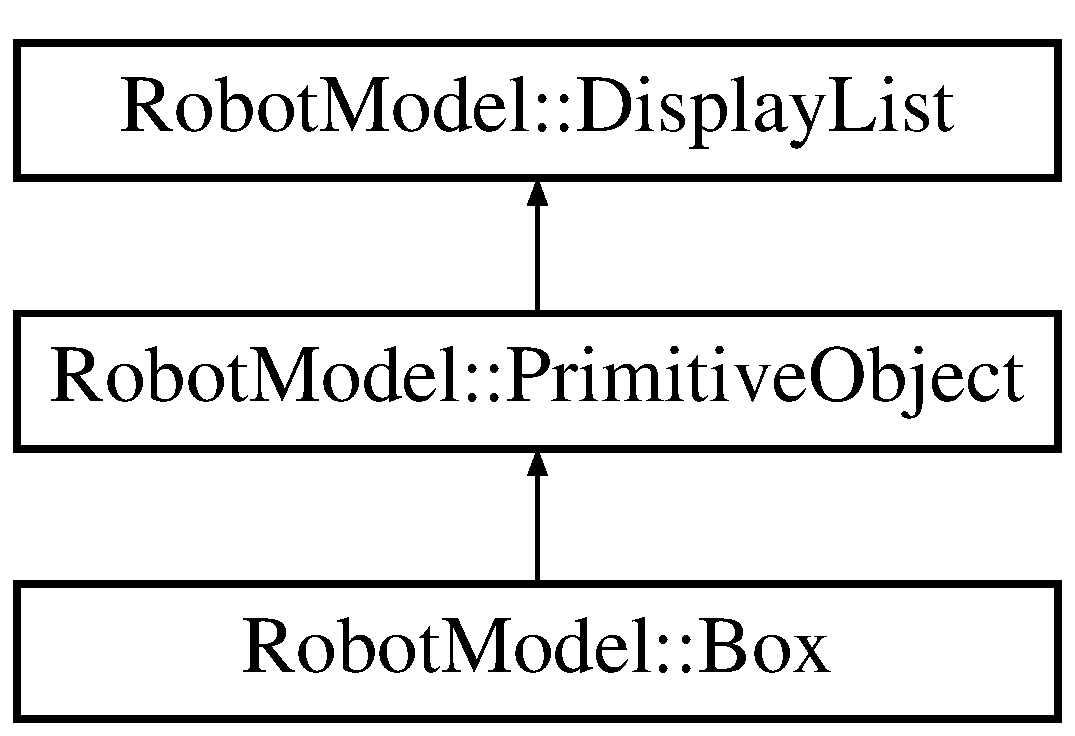
\includegraphics[height=2.35955cm]{class_robot_model_1_1_box}
\end{center}
\end{figure}
\subsection*{Public Member Functions}
\begin{DoxyCompactItemize}
\item 
\hyperlink{class_robot_model_1_1_box_a4f394975b4dadbd1fa34d124f33772cb}{Box} (const QVector3D \&size)
\item 
\hyperlink{class_robot_model_1_1_box_a6a5e09398e85d602a046b429062fb9c2}{$\sim$Box} ()
\item 
virtual void \hyperlink{class_robot_model_1_1_box_a29420d81c8b3622c95a1976593e2cc4b}{makeDisplayList} ()
\item 
\hyperlink{class_robot_model_1_1_box_a045eb20c935ee6c2b35213c7163f2418}{Box} (const QVector3D \&size)
\item 
\hyperlink{class_robot_model_1_1_box_af171ccea0a183894859a77ed105aeff6}{$\sim$Box} ()
\item 
virtual void \hyperlink{class_robot_model_1_1_box_a9499dafbda230821b419e3f578316d91}{makeDisplayList} ()
\end{DoxyCompactItemize}


\subsection{Constructor \& Destructor Documentation}
\hypertarget{class_robot_model_1_1_box_a4f394975b4dadbd1fa34d124f33772cb}{
\index{RobotModel::Box@{RobotModel::Box}!Box@{Box}}
\index{Box@{Box}!RobotModel::Box@{RobotModel::Box}}
\subsubsection[{Box}]{\setlength{\rightskip}{0pt plus 5cm}Box::Box (const QVector3D \& {\em size})}}
\label{class_robot_model_1_1_box_a4f394975b4dadbd1fa34d124f33772cb}
\hypertarget{class_robot_model_1_1_box_a6a5e09398e85d602a046b429062fb9c2}{
\index{RobotModel::Box@{RobotModel::Box}!$\sim$Box@{$\sim$Box}}
\index{$\sim$Box@{$\sim$Box}!RobotModel::Box@{RobotModel::Box}}
\subsubsection[{$\sim$Box}]{\setlength{\rightskip}{0pt plus 5cm}Box::$\sim$Box ()}}
\label{class_robot_model_1_1_box_a6a5e09398e85d602a046b429062fb9c2}
\hypertarget{class_robot_model_1_1_box_a045eb20c935ee6c2b35213c7163f2418}{
\index{RobotModel::Box@{RobotModel::Box}!Box@{Box}}
\index{Box@{Box}!RobotModel::Box@{RobotModel::Box}}
\subsubsection[{Box}]{\setlength{\rightskip}{0pt plus 5cm}RobotModel::Box::Box (const QVector3D \& {\em size})}}
\label{class_robot_model_1_1_box_a045eb20c935ee6c2b35213c7163f2418}
\hypertarget{class_robot_model_1_1_box_af171ccea0a183894859a77ed105aeff6}{
\index{RobotModel::Box@{RobotModel::Box}!$\sim$Box@{$\sim$Box}}
\index{$\sim$Box@{$\sim$Box}!RobotModel::Box@{RobotModel::Box}}
\subsubsection[{$\sim$Box}]{\setlength{\rightskip}{0pt plus 5cm}RobotModel::Box::$\sim$Box ()}}
\label{class_robot_model_1_1_box_af171ccea0a183894859a77ed105aeff6}


\subsection{Member Function Documentation}
\hypertarget{class_robot_model_1_1_box_a9499dafbda230821b419e3f578316d91}{
\index{RobotModel::Box@{RobotModel::Box}!makeDisplayList@{makeDisplayList}}
\index{makeDisplayList@{makeDisplayList}!RobotModel::Box@{RobotModel::Box}}
\subsubsection[{makeDisplayList}]{\setlength{\rightskip}{0pt plus 5cm}virtual void RobotModel::Box::makeDisplayList ()\hspace{0.3cm}{\ttfamily  \mbox{[}virtual\mbox{]}}}}
\label{class_robot_model_1_1_box_a9499dafbda230821b419e3f578316d91}


Implements \hyperlink{class_robot_model_1_1_display_list_a842de97924298c7363e50aebd69e5a50}{RobotModel::DisplayList}.\hypertarget{class_robot_model_1_1_box_a29420d81c8b3622c95a1976593e2cc4b}{
\index{RobotModel::Box@{RobotModel::Box}!makeDisplayList@{makeDisplayList}}
\index{makeDisplayList@{makeDisplayList}!RobotModel::Box@{RobotModel::Box}}
\subsubsection[{makeDisplayList}]{\setlength{\rightskip}{0pt plus 5cm}void Box::makeDisplayList ()\hspace{0.3cm}{\ttfamily  \mbox{[}virtual\mbox{]}}}}
\label{class_robot_model_1_1_box_a29420d81c8b3622c95a1976593e2cc4b}


Implements \hyperlink{class_robot_model_1_1_display_list_a842de97924298c7363e50aebd69e5a50}{RobotModel::DisplayList}.

The documentation for this class was generated from the following files:\begin{DoxyCompactItemize}
\item 
/Users/kail/imClever/dev/virtualSkin/include/robotModel/\hyperlink{include_2robot_model_2box_8h}{box.h}\item 
/Users/kail/imClever/dev/virtualSkin/src/robotModel/\hyperlink{src_2robot_model_2box_8h}{box.h}\item 
/Users/kail/imClever/dev/virtualSkin/src/robotModel/\hyperlink{box_8cpp}{box.cpp}\end{DoxyCompactItemize}

\hypertarget{class_call_observer}{
\section{CallObserver Class Reference}
\label{class_call_observer}\index{CallObserver@{CallObserver}}
}


{\ttfamily \#include $<$CallObserver.h$>$}Inheritance diagram for CallObserver::\begin{figure}[H]
\begin{center}
\leavevmode
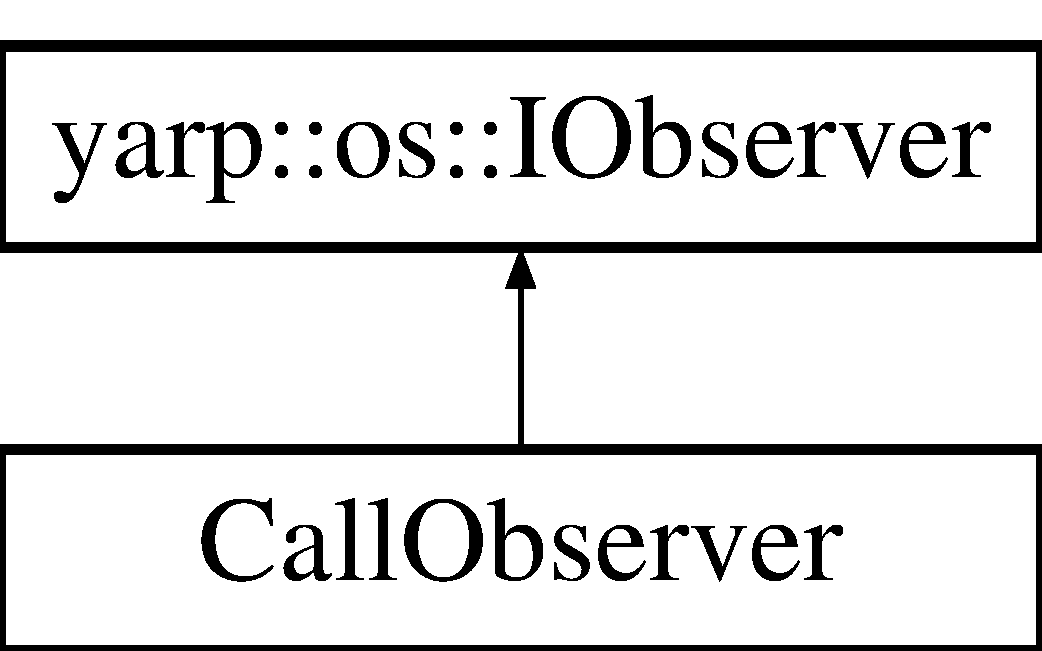
\includegraphics[height=2cm]{class_call_observer}
\end{center}
\end{figure}
\subsection*{Public Member Functions}
\begin{DoxyCompactItemize}
\item 
\hyperlink{class_call_observer_abc4eedb5f415fe0573cbd652554a5cd3}{CallObserver} (\hyperlink{class_robot_model_1_1_robot}{RobotModel::Robot} $\ast$r, const int b)
\item 
virtual \hyperlink{class_call_observer_aa357a50f75f42bfc944af11f41265fee}{$\sim$CallObserver} ()
\item 
virtual void \hyperlink{class_call_observer_abc1974fe2f04101dbbb1ae3ce83e7bfe}{onDataObserved} (yarp::os::Bottle \&b)
\item 
void \hyperlink{class_call_observer_a7551cd8674e37faa25451d78150f6a7c}{setResponseObsever} (\hyperlink{class_response_observer}{ResponseObserver} $\ast$o)
\end{DoxyCompactItemize}


\subsection{Constructor \& Destructor Documentation}
\hypertarget{class_call_observer_abc4eedb5f415fe0573cbd652554a5cd3}{
\index{CallObserver@{CallObserver}!CallObserver@{CallObserver}}
\index{CallObserver@{CallObserver}!CallObserver@{CallObserver}}
\subsubsection[{CallObserver}]{\setlength{\rightskip}{0pt plus 5cm}CallObserver::CallObserver ({\bf RobotModel::Robot} $\ast$ {\em r}, \/  const int {\em b})}}
\label{class_call_observer_abc4eedb5f415fe0573cbd652554a5cd3}
\hypertarget{class_call_observer_aa357a50f75f42bfc944af11f41265fee}{
\index{CallObserver@{CallObserver}!$\sim$CallObserver@{$\sim$CallObserver}}
\index{$\sim$CallObserver@{$\sim$CallObserver}!CallObserver@{CallObserver}}
\subsubsection[{$\sim$CallObserver}]{\setlength{\rightskip}{0pt plus 5cm}CallObserver::$\sim$CallObserver ()\hspace{0.3cm}{\ttfamily  \mbox{[}virtual\mbox{]}}}}
\label{class_call_observer_aa357a50f75f42bfc944af11f41265fee}


\subsection{Member Function Documentation}
\hypertarget{class_call_observer_abc1974fe2f04101dbbb1ae3ce83e7bfe}{
\index{CallObserver@{CallObserver}!onDataObserved@{onDataObserved}}
\index{onDataObserved@{onDataObserved}!CallObserver@{CallObserver}}
\subsubsection[{onDataObserved}]{\setlength{\rightskip}{0pt plus 5cm}void CallObserver::onDataObserved (yarp::os::Bottle \& {\em b})\hspace{0.3cm}{\ttfamily  \mbox{[}virtual\mbox{]}}}}
\label{class_call_observer_abc1974fe2f04101dbbb1ae3ce83e7bfe}
This function is called by filters to inform the implementing objects on data flowing in or out a the calling filter (RpcFilter as well as StreamFilter). 

Implements \hyperlink{classyarp_1_1os_1_1_i_observer_a4829e5a6f2ba6666b9539a4a30f20790}{yarp::os::IObserver}.\hypertarget{class_call_observer_a7551cd8674e37faa25451d78150f6a7c}{
\index{CallObserver@{CallObserver}!setResponseObsever@{setResponseObsever}}
\index{setResponseObsever@{setResponseObsever}!CallObserver@{CallObserver}}
\subsubsection[{setResponseObsever}]{\setlength{\rightskip}{0pt plus 5cm}void CallObserver::setResponseObsever ({\bf ResponseObserver} $\ast$ {\em o})}}
\label{class_call_observer_a7551cd8674e37faa25451d78150f6a7c}


The documentation for this class was generated from the following files:\begin{DoxyCompactItemize}
\item 
/Users/kail/imClever/dev/virtualSkin/src/reflex/\hyperlink{_call_observer_8h}{CallObserver.h}\item 
/Users/kail/imClever/dev/virtualSkin/src/reflex/\hyperlink{_call_observer_8cpp}{CallObserver.cpp}\end{DoxyCompactItemize}

\hypertarget{class_circular_buffer}{
\section{CircularBuffer Class Reference}
\label{class_circular_buffer}\index{CircularBuffer@{CircularBuffer}}
}


{\ttfamily \#include $<$circularBuffer.h$>$}\subsection*{Public Member Functions}
\begin{DoxyCompactItemize}
\item 
\hyperlink{class_circular_buffer_a8c5de0e610bb50bac684f4707e23431c}{CircularBuffer} ()
\item 
\hyperlink{class_circular_buffer_a916f9506cf86010056d189b51fd72c91}{$\sim$CircularBuffer} ()
\item 
void \hyperlink{class_circular_buffer_ae9f2d25b6b0a7f2eda25147a0bfbac93}{setBufferSize} (int bufferLength)
\item 
void \hyperlink{class_circular_buffer_aa79025f00e3b84355eb037a5755b2700}{init} (const QVector$<$ qreal $>$)
\item 
void \hyperlink{class_circular_buffer_a279c6c54d6a7f1f94d3d5311dc8a631f}{put} (const QVector$<$ qreal $>$)
\item 
void \hyperlink{class_circular_buffer_aa90e1d3b23077235958bfc60e7b02805}{next} ()
\item 
QVector$<$ qreal $>$ \& \hyperlink{class_circular_buffer_a9f6b11ef3601e32beac4d5525211ce52}{getOldest} ()
\item 
QVector$<$ qreal $>$ \& \hyperlink{class_circular_buffer_a7c4096d1efc8e1cdc9f5be5be3c349e1}{getCurrent} ()
\end{DoxyCompactItemize}


\subsection{Constructor \& Destructor Documentation}
\hypertarget{class_circular_buffer_a8c5de0e610bb50bac684f4707e23431c}{
\index{CircularBuffer@{CircularBuffer}!CircularBuffer@{CircularBuffer}}
\index{CircularBuffer@{CircularBuffer}!CircularBuffer@{CircularBuffer}}
\subsubsection[{CircularBuffer}]{\setlength{\rightskip}{0pt plus 5cm}CircularBuffer::CircularBuffer ()}}
\label{class_circular_buffer_a8c5de0e610bb50bac684f4707e23431c}
\hypertarget{class_circular_buffer_a916f9506cf86010056d189b51fd72c91}{
\index{CircularBuffer@{CircularBuffer}!$\sim$CircularBuffer@{$\sim$CircularBuffer}}
\index{$\sim$CircularBuffer@{$\sim$CircularBuffer}!CircularBuffer@{CircularBuffer}}
\subsubsection[{$\sim$CircularBuffer}]{\setlength{\rightskip}{0pt plus 5cm}CircularBuffer::$\sim$CircularBuffer ()}}
\label{class_circular_buffer_a916f9506cf86010056d189b51fd72c91}


\subsection{Member Function Documentation}
\hypertarget{class_circular_buffer_a7c4096d1efc8e1cdc9f5be5be3c349e1}{
\index{CircularBuffer@{CircularBuffer}!getCurrent@{getCurrent}}
\index{getCurrent@{getCurrent}!CircularBuffer@{CircularBuffer}}
\subsubsection[{getCurrent}]{\setlength{\rightskip}{0pt plus 5cm}QVector$<$ qreal $>$ \& CircularBuffer::getCurrent ()}}
\label{class_circular_buffer_a7c4096d1efc8e1cdc9f5be5be3c349e1}
\hypertarget{class_circular_buffer_a9f6b11ef3601e32beac4d5525211ce52}{
\index{CircularBuffer@{CircularBuffer}!getOldest@{getOldest}}
\index{getOldest@{getOldest}!CircularBuffer@{CircularBuffer}}
\subsubsection[{getOldest}]{\setlength{\rightskip}{0pt plus 5cm}QVector$<$ qreal $>$ \& CircularBuffer::getOldest ()}}
\label{class_circular_buffer_a9f6b11ef3601e32beac4d5525211ce52}
\hypertarget{class_circular_buffer_aa79025f00e3b84355eb037a5755b2700}{
\index{CircularBuffer@{CircularBuffer}!init@{init}}
\index{init@{init}!CircularBuffer@{CircularBuffer}}
\subsubsection[{init}]{\setlength{\rightskip}{0pt plus 5cm}void CircularBuffer::init (const QVector$<$ qreal $>$ {\em v})}}
\label{class_circular_buffer_aa79025f00e3b84355eb037a5755b2700}
\hypertarget{class_circular_buffer_aa90e1d3b23077235958bfc60e7b02805}{
\index{CircularBuffer@{CircularBuffer}!next@{next}}
\index{next@{next}!CircularBuffer@{CircularBuffer}}
\subsubsection[{next}]{\setlength{\rightskip}{0pt plus 5cm}void CircularBuffer::next ()}}
\label{class_circular_buffer_aa90e1d3b23077235958bfc60e7b02805}
\hypertarget{class_circular_buffer_a279c6c54d6a7f1f94d3d5311dc8a631f}{
\index{CircularBuffer@{CircularBuffer}!put@{put}}
\index{put@{put}!CircularBuffer@{CircularBuffer}}
\subsubsection[{put}]{\setlength{\rightskip}{0pt plus 5cm}void CircularBuffer::put (const QVector$<$ qreal $>$ {\em v})}}
\label{class_circular_buffer_a279c6c54d6a7f1f94d3d5311dc8a631f}
\hypertarget{class_circular_buffer_ae9f2d25b6b0a7f2eda25147a0bfbac93}{
\index{CircularBuffer@{CircularBuffer}!setBufferSize@{setBufferSize}}
\index{setBufferSize@{setBufferSize}!CircularBuffer@{CircularBuffer}}
\subsubsection[{setBufferSize}]{\setlength{\rightskip}{0pt plus 5cm}void CircularBuffer::setBufferSize (int {\em bufferLength})}}
\label{class_circular_buffer_ae9f2d25b6b0a7f2eda25147a0bfbac93}


The documentation for this class was generated from the following files:\begin{DoxyCompactItemize}
\item 
/Users/kail/imClever/dev/virtualSkin/src/reflex/\hyperlink{circular_buffer_8h}{circularBuffer.h}\item 
/Users/kail/imClever/dev/virtualSkin/src/reflex/\hyperlink{circular_buffer_8cpp}{circularBuffer.cpp}\end{DoxyCompactItemize}

\hypertarget{class_collision_detector}{
\section{CollisionDetector Class Reference}
\label{class_collision_detector}\index{CollisionDetector@{CollisionDetector}}
}


Computes the current pose of the Robot and does collision detection using the FreeSOLID library.  


{\ttfamily \#include $<$collisionDetector.h$>$}\subsection*{Public Slots}
\begin{DoxyCompactItemize}
\item 
void \hyperlink{class_collision_detector_ad75885bcd649c22da007c91e91b17dfc}{armDetector} ()
\begin{DoxyCompactList}\small\item\em When armed, the collisionDetector will emit the \hyperlink{class_collision_detector_a7a6c1a9b11907db7252b6544ee1ce8b4}{crash()} signal if collision(s) occurr(s). \item\end{DoxyCompactList}\item 
void \hyperlink{class_collision_detector_a0ff5daf20c76c64a2e284f93bd5e50a3}{disarmDetector} ()
\begin{DoxyCompactList}\small\item\em When disarmed, the collisionDetector will not emit the \hyperlink{class_collision_detector_a7a6c1a9b11907db7252b6544ee1ce8b4}{crash()} signal regardless. \item\end{DoxyCompactList}\item 
bool \hyperlink{class_collision_detector_a92faad68f69ade7020a58f105f7d3aa8}{computePose} ()
\begin{DoxyCompactList}\small\item\em Causes the Robot's pose to be computed in cartesian space and the collision detection to be run using FreeSOLID. \item\end{DoxyCompactList}\end{DoxyCompactItemize}
\subsection*{Signals}
\begin{DoxyCompactItemize}
\item 
void \hyperlink{class_collision_detector_a9540d0ce34c4721abb8bf9bfcb1f67dd}{newPoseReady} ()
\begin{DoxyCompactList}\small\item\em Signifies that a new pose (in cartesian space) has been computed. \item\end{DoxyCompactList}\item 
void \hyperlink{class_collision_detector_a7a6c1a9b11907db7252b6544ee1ce8b4}{crash} ()
\begin{DoxyCompactList}\small\item\em Signifies that a collision(s) has/have occurred. \item\end{DoxyCompactList}\end{DoxyCompactItemize}
\subsection*{Public Member Functions}
\begin{DoxyCompactItemize}
\item 
\hyperlink{class_collision_detector_ab3f66bd8d272a21674e38bf46d4d31e0}{CollisionDetector} ()
\begin{DoxyCompactList}\small\item\em Constructs an armed collisionDetector object. \item\end{DoxyCompactList}\item 
\hyperlink{class_collision_detector_a1a0f7a386920e0cf83a101be92f04598}{$\sim$CollisionDetector} ()
\begin{DoxyCompactList}\small\item\em Just stops the YARP port if its running. \item\end{DoxyCompactList}\item 
void \hyperlink{class_collision_detector_a2c768facee0187d691dcc268b91d9652}{setRobot} (\hyperlink{class_robot_model_1_1_robot}{RobotModel::Robot} $\ast$aRobot)
\begin{DoxyCompactList}\small\item\em Binds this collision detector to a robot model. \item\end{DoxyCompactList}\item 
void \hyperlink{class_collision_detector_a7490b9d8f95f73b55b3add14ea58a737}{setWorld} (\hyperlink{class_robot_model_1_1_world}{RobotModel::World} $\ast$aWorld)
\begin{DoxyCompactList}\small\item\em Binds this collision detector to a world model. \item\end{DoxyCompactList}\item 
void \hyperlink{class_collision_detector_acd233230c6fd897f206e1fe016b7521d}{setPortName} (const QString \&aName)
\begin{DoxyCompactList}\small\item\em Sets the name of the YARP stream port where collision info will be published. \item\end{DoxyCompactList}\item 
void \hyperlink{class_collision_detector_a1fa9e503fff5d46bd3b068dc8cd98fe4}{openPort} ()
\begin{DoxyCompactList}\small\item\em Opens the YARP stream port. \item\end{DoxyCompactList}\item 
void \hyperlink{class_collision_detector_a2a9b9c210d15989278ec9ff3e88b67c7}{closePort} ()
\begin{DoxyCompactList}\small\item\em Closes the YARP stream port. \item\end{DoxyCompactList}\item 
bool \hyperlink{class_collision_detector_adda71d45cdd4a428945f6a8e9c750296}{detectorIsArmed} ()
\begin{DoxyCompactList}\small\item\em Returns whether or not the collisionDetector is armed. \item\end{DoxyCompactList}\end{DoxyCompactItemize}
\subsection*{Static Public Member Functions}
\begin{DoxyCompactItemize}
\item 
static void \hyperlink{class_collision_detector_a4899ce7cf1ba8c2efe37329e49aff128}{collisionHandler} (void $\ast$client\_\-data, DtObjectRef obj1, DtObjectRef obj2, const DtCollData $\ast$coll\_\-data)
\end{DoxyCompactItemize}


\subsection{Detailed Description}
Computes the current pose of the Robot and does collision detection using the FreeSOLID library. To use this class: First prepare the object by calling the constructor, setRobot(Robot$\ast$) and setWorld(World$\ast$). If you want to publish collision information on the network via YARP, call setPortName(QString\&) and \hyperlink{class_collision_detector_a1fa9e503fff5d46bd3b068dc8cd98fe4}{openPort()}. Call/activate the slot \hyperlink{class_collision_detector_a92faad68f69ade7020a58f105f7d3aa8}{computePose()} when you suspect the robot's state has changed. When the pose has been computed and collision detection is finished, the signal \hyperlink{class_collision_detector_a9540d0ce34c4721abb8bf9bfcb1f67dd}{newPoseReady()} will be emitted. If one or more collisions have occurred, the signal \hyperlink{class_collision_detector_a7a6c1a9b11907db7252b6544ee1ce8b4}{crash()} will also be emitted, provided that the \hyperlink{class_collision_detector}{CollisionDetector} is armed. Finally, use the slots \hyperlink{class_collision_detector_ad75885bcd649c22da007c91e91b17dfc}{armDetector()} and \hyperlink{class_collision_detector_a0ff5daf20c76c64a2e284f93bd5e50a3}{disarmDetector()} to control whether or not to emit the \hyperlink{class_collision_detector_a7a6c1a9b11907db7252b6544ee1ce8b4}{crash()} signal if a collision has occurred. This is useful if the \hyperlink{class_collision_detector_a7a6c1a9b11907db7252b6544ee1ce8b4}{crash()} signal triggers some kind of collision handling control code, as you can supress subsequent crash signals until the collision handling is complete.

NOTE: Collision detection is only carried out between the robot and itself O(n$^\wedge$2) where n=$|$robot$|$, as well as between the robot and the world O(n) where n=$|$world$|$. Thus the computational complexity of the collision detection grows linearly with the size of the world. 

\subsection{Constructor \& Destructor Documentation}
\hypertarget{class_collision_detector_ab3f66bd8d272a21674e38bf46d4d31e0}{
\index{CollisionDetector@{CollisionDetector}!CollisionDetector@{CollisionDetector}}
\index{CollisionDetector@{CollisionDetector}!CollisionDetector@{CollisionDetector}}
\subsubsection[{CollisionDetector}]{\setlength{\rightskip}{0pt plus 5cm}CollisionDetector::CollisionDetector ()}}
\label{class_collision_detector_ab3f66bd8d272a21674e38bf46d4d31e0}


Constructs an armed collisionDetector object. \hypertarget{class_collision_detector_a1a0f7a386920e0cf83a101be92f04598}{
\index{CollisionDetector@{CollisionDetector}!$\sim$CollisionDetector@{$\sim$CollisionDetector}}
\index{$\sim$CollisionDetector@{$\sim$CollisionDetector}!CollisionDetector@{CollisionDetector}}
\subsubsection[{$\sim$CollisionDetector}]{\setlength{\rightskip}{0pt plus 5cm}CollisionDetector::$\sim$CollisionDetector ()}}
\label{class_collision_detector_a1a0f7a386920e0cf83a101be92f04598}


Just stops the YARP port if its running. 

\subsection{Member Function Documentation}
\hypertarget{class_collision_detector_ad75885bcd649c22da007c91e91b17dfc}{
\index{CollisionDetector@{CollisionDetector}!armDetector@{armDetector}}
\index{armDetector@{armDetector}!CollisionDetector@{CollisionDetector}}
\subsubsection[{armDetector}]{\setlength{\rightskip}{0pt plus 5cm}void CollisionDetector::armDetector ()\hspace{0.3cm}{\ttfamily  \mbox{[}slot\mbox{]}}}}
\label{class_collision_detector_ad75885bcd649c22da007c91e91b17dfc}


When armed, the collisionDetector will emit the \hyperlink{class_collision_detector_a7a6c1a9b11907db7252b6544ee1ce8b4}{crash()} signal if collision(s) occurr(s). \hypertarget{class_collision_detector_a2a9b9c210d15989278ec9ff3e88b67c7}{
\index{CollisionDetector@{CollisionDetector}!closePort@{closePort}}
\index{closePort@{closePort}!CollisionDetector@{CollisionDetector}}
\subsubsection[{closePort}]{\setlength{\rightskip}{0pt plus 5cm}void CollisionDetector::closePort ()\hspace{0.3cm}{\ttfamily  \mbox{[}inline\mbox{]}}}}
\label{class_collision_detector_a2a9b9c210d15989278ec9ff3e88b67c7}


Closes the YARP stream port. \hypertarget{class_collision_detector_a4899ce7cf1ba8c2efe37329e49aff128}{
\index{CollisionDetector@{CollisionDetector}!collisionHandler@{collisionHandler}}
\index{collisionHandler@{collisionHandler}!CollisionDetector@{CollisionDetector}}
\subsubsection[{collisionHandler}]{\setlength{\rightskip}{0pt plus 5cm}static void CollisionDetector::collisionHandler (void $\ast$ {\em client\_\-data}, \/  DtObjectRef {\em obj1}, \/  DtObjectRef {\em obj2}, \/  const DtCollData $\ast$ {\em coll\_\-data})\hspace{0.3cm}{\ttfamily  \mbox{[}inline, static\mbox{]}}}}
\label{class_collision_detector_a4899ce7cf1ba8c2efe37329e49aff128}
This callback is executed whenever FreeSOLID encounters a collision between Objects. It sets a flag that collision(s) has/have occurred, and encodes the collision state into a YARP bottle. \hypertarget{class_collision_detector_a92faad68f69ade7020a58f105f7d3aa8}{
\index{CollisionDetector@{CollisionDetector}!computePose@{computePose}}
\index{computePose@{computePose}!CollisionDetector@{CollisionDetector}}
\subsubsection[{computePose}]{\setlength{\rightskip}{0pt plus 5cm}bool CollisionDetector::computePose ()\hspace{0.3cm}{\ttfamily  \mbox{[}slot\mbox{]}}}}
\label{class_collision_detector_a92faad68f69ade7020a58f105f7d3aa8}


Causes the Robot's pose to be computed in cartesian space and the collision detection to be run using FreeSOLID. \hypertarget{class_collision_detector_a7a6c1a9b11907db7252b6544ee1ce8b4}{
\index{CollisionDetector@{CollisionDetector}!crash@{crash}}
\index{crash@{crash}!CollisionDetector@{CollisionDetector}}
\subsubsection[{crash}]{\setlength{\rightskip}{0pt plus 5cm}void CollisionDetector::crash ()\hspace{0.3cm}{\ttfamily  \mbox{[}signal\mbox{]}}}}
\label{class_collision_detector_a7a6c1a9b11907db7252b6544ee1ce8b4}


Signifies that a collision(s) has/have occurred. \hypertarget{class_collision_detector_adda71d45cdd4a428945f6a8e9c750296}{
\index{CollisionDetector@{CollisionDetector}!detectorIsArmed@{detectorIsArmed}}
\index{detectorIsArmed@{detectorIsArmed}!CollisionDetector@{CollisionDetector}}
\subsubsection[{detectorIsArmed}]{\setlength{\rightskip}{0pt plus 5cm}bool CollisionDetector::detectorIsArmed ()\hspace{0.3cm}{\ttfamily  \mbox{[}inline\mbox{]}}}}
\label{class_collision_detector_adda71d45cdd4a428945f6a8e9c750296}


Returns whether or not the collisionDetector is armed. \hypertarget{class_collision_detector_a0ff5daf20c76c64a2e284f93bd5e50a3}{
\index{CollisionDetector@{CollisionDetector}!disarmDetector@{disarmDetector}}
\index{disarmDetector@{disarmDetector}!CollisionDetector@{CollisionDetector}}
\subsubsection[{disarmDetector}]{\setlength{\rightskip}{0pt plus 5cm}void CollisionDetector::disarmDetector ()\hspace{0.3cm}{\ttfamily  \mbox{[}inline, slot\mbox{]}}}}
\label{class_collision_detector_a0ff5daf20c76c64a2e284f93bd5e50a3}


When disarmed, the collisionDetector will not emit the \hyperlink{class_collision_detector_a7a6c1a9b11907db7252b6544ee1ce8b4}{crash()} signal regardless. \hypertarget{class_collision_detector_a9540d0ce34c4721abb8bf9bfcb1f67dd}{
\index{CollisionDetector@{CollisionDetector}!newPoseReady@{newPoseReady}}
\index{newPoseReady@{newPoseReady}!CollisionDetector@{CollisionDetector}}
\subsubsection[{newPoseReady}]{\setlength{\rightskip}{0pt plus 5cm}void CollisionDetector::newPoseReady ()\hspace{0.3cm}{\ttfamily  \mbox{[}signal\mbox{]}}}}
\label{class_collision_detector_a9540d0ce34c4721abb8bf9bfcb1f67dd}


Signifies that a new pose (in cartesian space) has been computed. \hypertarget{class_collision_detector_a1fa9e503fff5d46bd3b068dc8cd98fe4}{
\index{CollisionDetector@{CollisionDetector}!openPort@{openPort}}
\index{openPort@{openPort}!CollisionDetector@{CollisionDetector}}
\subsubsection[{openPort}]{\setlength{\rightskip}{0pt plus 5cm}void CollisionDetector::openPort ()}}
\label{class_collision_detector_a1fa9e503fff5d46bd3b068dc8cd98fe4}


Opens the YARP stream port. \hypertarget{class_collision_detector_acd233230c6fd897f206e1fe016b7521d}{
\index{CollisionDetector@{CollisionDetector}!setPortName@{setPortName}}
\index{setPortName@{setPortName}!CollisionDetector@{CollisionDetector}}
\subsubsection[{setPortName}]{\setlength{\rightskip}{0pt plus 5cm}void CollisionDetector::setPortName (const QString \& {\em aName})\hspace{0.3cm}{\ttfamily  \mbox{[}inline\mbox{]}}}}
\label{class_collision_detector_acd233230c6fd897f206e1fe016b7521d}


Sets the name of the YARP stream port where collision info will be published. \hypertarget{class_collision_detector_a2c768facee0187d691dcc268b91d9652}{
\index{CollisionDetector@{CollisionDetector}!setRobot@{setRobot}}
\index{setRobot@{setRobot}!CollisionDetector@{CollisionDetector}}
\subsubsection[{setRobot}]{\setlength{\rightskip}{0pt plus 5cm}void CollisionDetector::setRobot ({\bf RobotModel::Robot} $\ast$ {\em aRobot})\hspace{0.3cm}{\ttfamily  \mbox{[}inline\mbox{]}}}}
\label{class_collision_detector_a2c768facee0187d691dcc268b91d9652}


Binds this collision detector to a robot model. \hypertarget{class_collision_detector_a7490b9d8f95f73b55b3add14ea58a737}{
\index{CollisionDetector@{CollisionDetector}!setWorld@{setWorld}}
\index{setWorld@{setWorld}!CollisionDetector@{CollisionDetector}}
\subsubsection[{setWorld}]{\setlength{\rightskip}{0pt plus 5cm}void CollisionDetector::setWorld ({\bf RobotModel::World} $\ast$ {\em aWorld})\hspace{0.3cm}{\ttfamily  \mbox{[}inline\mbox{]}}}}
\label{class_collision_detector_a7490b9d8f95f73b55b3add14ea58a737}


Binds this collision detector to a world model. 

The documentation for this class was generated from the following files:\begin{DoxyCompactItemize}
\item 
/Users/kail/imClever/dev/virtualSkin/src/reflex/\hyperlink{collision_detector_8h}{collisionDetector.h}\item 
/Users/kail/imClever/dev/virtualSkin/src/reflex/\hyperlink{collision_detector_8cpp}{collisionDetector.cpp}\end{DoxyCompactItemize}

\hypertarget{class_robot_model_1_1_composite_object}{
\section{RobotModel::CompositeObject Class Reference}
\label{class_robot_model_1_1_composite_object}\index{RobotModel::CompositeObject@{RobotModel::CompositeObject}}
}


{\ttfamily \#include $<$object.h$>$}Inheritance diagram for RobotModel::CompositeObject::\begin{figure}[H]
\begin{center}
\leavevmode
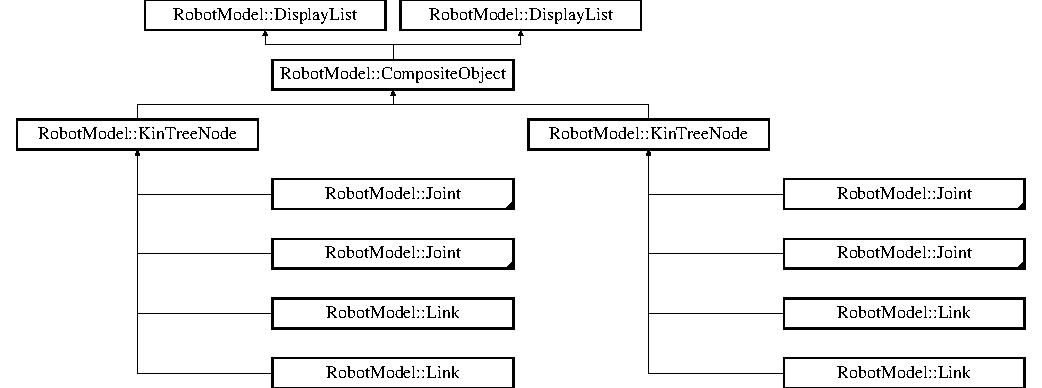
\includegraphics[height=4.96454cm]{class_robot_model_1_1_composite_object}
\end{center}
\end{figure}
\subsection*{Public Member Functions}
\begin{DoxyCompactItemize}
\item 
\hyperlink{class_robot_model_1_1_composite_object_a28feebceeaeec6c4d4ec6adc9fc52d90}{CompositeObject} (const QString \&aName=\char`\"{}unnamedObject\char`\"{})
\item 
virtual \hyperlink{class_robot_model_1_1_composite_object_a52c02078b1e3e9f4f436874fb044a27b}{$\sim$CompositeObject} ()
\item 
void \hyperlink{class_robot_model_1_1_composite_object_a02a2c1ee58297a6ea0131fa808498a49}{setName} (const QString \&aName)
\item 
const QString \& \hyperlink{class_robot_model_1_1_composite_object_a893e71523b76afc186796fc95ead70d7}{getName} ()
\item 
\hyperlink{class_robot_model_1_1_primitive_object}{PrimitiveObject} $\ast$ \hyperlink{class_robot_model_1_1_composite_object_aa5b61818415089630ee37a3767b5c37c}{newSphere} (double r, const QVector3D \&pos=QVector3D(0, 0, 0))
\item 
\hyperlink{class_robot_model_1_1_primitive_object}{PrimitiveObject} $\ast$ \hyperlink{class_robot_model_1_1_composite_object_a196a2811a85c1313f781b140f2ab313e}{newCylinder} (double r, double h, const QVector3D \&pos=QVector3D(0, 0, 0))
\item 
\hyperlink{class_robot_model_1_1_primitive_object}{PrimitiveObject} $\ast$ \hyperlink{class_robot_model_1_1_composite_object_a869235cebecc6802b9c63ce7e2359ddb}{newBox} (const QVector3D \&size, const QVector3D \&pos=QVector3D(0, 0, 0))
\item 
virtual void \hyperlink{class_robot_model_1_1_composite_object_ad33452f1246939d366ffbf02d1022a91}{append} (\hyperlink{class_robot_model_1_1_primitive_object}{PrimitiveObject} $\ast$primitiveObject)
\item 
\hyperlink{class_robot_model_1_1_primitive_object}{PrimitiveObject} $\ast$ \hyperlink{class_robot_model_1_1_composite_object_ad02b7a8e84453fb433d5efaac80333c9}{getPrimitiveByName} (const QString \&\hyperlink{class_robot_model_1_1_composite_object_a4e833bb302d4a1a791211261251eff68}{objectName}) const 
\item 
virtual bool \hyperlink{class_robot_model_1_1_composite_object_ac63de1955b6bda820d39c01616af8665}{remove} (\hyperlink{class_robot_model_1_1_primitive_object}{PrimitiveObject} $\ast$primitive)
\item 
void \hyperlink{class_robot_model_1_1_composite_object_abd48ac40b21178f5306ddfa6c92ea3c3}{setT} (const QMatrix4x4 \&txfr)
\item 
void \hyperlink{class_robot_model_1_1_composite_object_a12e8961ebc63d8a253d915b29b356162}{setCartesianRotation} (const QVector3D \&rot)
\item 
void \hyperlink{class_robot_model_1_1_composite_object_adadc29cccbba9cb615eaf0ad2fbdd337}{cartesianRotate} (const QVector3D \&rot)
\item 
void \hyperlink{class_robot_model_1_1_composite_object_a43f99ed52def7114d310e29fc6db83f3}{setAxisAngleRotation} (const QVector3D \&axis, qreal angle)
\item 
void \hyperlink{class_robot_model_1_1_composite_object_a357f5ed3f49e0889df511271e468f866}{axisAngleRotate} (const QVector3D \&axis, qreal angle)
\item 
void \hyperlink{class_robot_model_1_1_composite_object_ad44b9c1759209367754dafd77c984d6f}{specialRotate} (const QVector3D \&axis, qreal angle=0)
\item 
void \hyperlink{class_robot_model_1_1_composite_object_ae925e59246174c9d3b74d459b32835e3}{setTranslation} (const QVector3D \&trans)
\item 
void \hyperlink{class_robot_model_1_1_composite_object_afd942b7fa3b18bcc01c3fba417a6c027}{translate} (const QVector3D \&trans)
\item 
void \hyperlink{class_robot_model_1_1_composite_object_a5aa475cb09f0e9b9089a941848f9e189}{makeDisplayList} ()
\item 
virtual void \hyperlink{class_robot_model_1_1_composite_object_aee43da74b22f6272736844effe7a1dd6}{render} ()
\item 
void \hyperlink{class_robot_model_1_1_composite_object_ab6dc53258a7cdb53a22af63688d50ddd}{doNotCheckCollision} (const \hyperlink{class_robot_model_1_1_composite_object}{CompositeObject} $\ast$a) const 
\item 
void \hyperlink{class_robot_model_1_1_composite_object_a788711732ec5994c3f3a09321e2c5a18}{doNotCheckCollision} (\hyperlink{class_robot_model_1_1_primitive_object}{PrimitiveObject} $\ast$a) const 
\item 
virtual void \hyperlink{class_robot_model_1_1_composite_object_a00db0d1a45893ef058e7abbad5083b6b}{notColliding} ()
\item 
virtual void \hyperlink{class_robot_model_1_1_composite_object_aacfefeee128f748e4e705708b9d958e3}{update} ()
\end{DoxyCompactItemize}
\subsection*{Protected Attributes}
\begin{DoxyCompactItemize}
\item 
QString \hyperlink{class_robot_model_1_1_composite_object_a4e833bb302d4a1a791211261251eff68}{objectName}
\item 
int \hyperlink{class_robot_model_1_1_composite_object_ad2f0b50dd12a6d6cba7d48c65266490a}{numSpheres}
\item 
int \hyperlink{class_robot_model_1_1_composite_object_a316bb31790aa7d8905a31523890187b3}{numCylinders}
\item 
int \hyperlink{class_robot_model_1_1_composite_object_a05fb383ad49f9da7da584b12804e4f19}{numBoxes}
\end{DoxyCompactItemize}


\subsection{Constructor \& Destructor Documentation}
\hypertarget{class_robot_model_1_1_composite_object_a28feebceeaeec6c4d4ec6adc9fc52d90}{
\index{RobotModel::CompositeObject@{RobotModel::CompositeObject}!CompositeObject@{CompositeObject}}
\index{CompositeObject@{CompositeObject}!RobotModel::CompositeObject@{RobotModel::CompositeObject}}
\subsubsection[{CompositeObject}]{\setlength{\rightskip}{0pt plus 5cm}CompositeObject::CompositeObject (const QString \& {\em aName} = {\ttfamily \char`\"{}unnamedObject\char`\"{}})}}
\label{class_robot_model_1_1_composite_object_a28feebceeaeec6c4d4ec6adc9fc52d90}
\hypertarget{class_robot_model_1_1_composite_object_a52c02078b1e3e9f4f436874fb044a27b}{
\index{RobotModel::CompositeObject@{RobotModel::CompositeObject}!$\sim$CompositeObject@{$\sim$CompositeObject}}
\index{$\sim$CompositeObject@{$\sim$CompositeObject}!RobotModel::CompositeObject@{RobotModel::CompositeObject}}
\subsubsection[{$\sim$CompositeObject}]{\setlength{\rightskip}{0pt plus 5cm}CompositeObject::$\sim$CompositeObject ()\hspace{0.3cm}{\ttfamily  \mbox{[}virtual\mbox{]}}}}
\label{class_robot_model_1_1_composite_object_a52c02078b1e3e9f4f436874fb044a27b}


\subsection{Member Function Documentation}
\hypertarget{class_robot_model_1_1_composite_object_ad33452f1246939d366ffbf02d1022a91}{
\index{RobotModel::CompositeObject@{RobotModel::CompositeObject}!append@{append}}
\index{append@{append}!RobotModel::CompositeObject@{RobotModel::CompositeObject}}
\subsubsection[{append}]{\setlength{\rightskip}{0pt plus 5cm}void CompositeObject::append ({\bf PrimitiveObject} $\ast$ {\em primitiveObject})\hspace{0.3cm}{\ttfamily  \mbox{[}virtual\mbox{]}}}}
\label{class_robot_model_1_1_composite_object_ad33452f1246939d366ffbf02d1022a91}


Reimplemented in \hyperlink{class_robot_model_1_1_kin_tree_node_af043fc57074a449364d2a6ec09be46a3}{RobotModel::KinTreeNode}.\hypertarget{class_robot_model_1_1_composite_object_a357f5ed3f49e0889df511271e468f866}{
\index{RobotModel::CompositeObject@{RobotModel::CompositeObject}!axisAngleRotate@{axisAngleRotate}}
\index{axisAngleRotate@{axisAngleRotate}!RobotModel::CompositeObject@{RobotModel::CompositeObject}}
\subsubsection[{axisAngleRotate}]{\setlength{\rightskip}{0pt plus 5cm}void CompositeObject::axisAngleRotate (const QVector3D \& {\em axis}, \/  qreal {\em angle})\hspace{0.3cm}{\ttfamily  \mbox{[}virtual\mbox{]}}}}
\label{class_robot_model_1_1_composite_object_a357f5ed3f49e0889df511271e468f866}


Reimplemented from \hyperlink{class_robot_model_1_1_display_list_a9a7084168997ac285ee1e9f4041a8d57}{RobotModel::DisplayList}.\hypertarget{class_robot_model_1_1_composite_object_adadc29cccbba9cb615eaf0ad2fbdd337}{
\index{RobotModel::CompositeObject@{RobotModel::CompositeObject}!cartesianRotate@{cartesianRotate}}
\index{cartesianRotate@{cartesianRotate}!RobotModel::CompositeObject@{RobotModel::CompositeObject}}
\subsubsection[{cartesianRotate}]{\setlength{\rightskip}{0pt plus 5cm}void CompositeObject::cartesianRotate (const QVector3D \& {\em rot})\hspace{0.3cm}{\ttfamily  \mbox{[}virtual\mbox{]}}}}
\label{class_robot_model_1_1_composite_object_adadc29cccbba9cb615eaf0ad2fbdd337}


Reimplemented from \hyperlink{class_robot_model_1_1_display_list_a023ba88eaac38b26dc9ea6a358467637}{RobotModel::DisplayList}.\hypertarget{class_robot_model_1_1_composite_object_a788711732ec5994c3f3a09321e2c5a18}{
\index{RobotModel::CompositeObject@{RobotModel::CompositeObject}!doNotCheckCollision@{doNotCheckCollision}}
\index{doNotCheckCollision@{doNotCheckCollision}!RobotModel::CompositeObject@{RobotModel::CompositeObject}}
\subsubsection[{doNotCheckCollision}]{\setlength{\rightskip}{0pt plus 5cm}void CompositeObject::doNotCheckCollision ({\bf PrimitiveObject} $\ast$ {\em a}) const}}
\label{class_robot_model_1_1_composite_object_a788711732ec5994c3f3a09321e2c5a18}
\hypertarget{class_robot_model_1_1_composite_object_ab6dc53258a7cdb53a22af63688d50ddd}{
\index{RobotModel::CompositeObject@{RobotModel::CompositeObject}!doNotCheckCollision@{doNotCheckCollision}}
\index{doNotCheckCollision@{doNotCheckCollision}!RobotModel::CompositeObject@{RobotModel::CompositeObject}}
\subsubsection[{doNotCheckCollision}]{\setlength{\rightskip}{0pt plus 5cm}void CompositeObject::doNotCheckCollision (const {\bf CompositeObject} $\ast$ {\em a}) const}}
\label{class_robot_model_1_1_composite_object_ab6dc53258a7cdb53a22af63688d50ddd}
\hypertarget{class_robot_model_1_1_composite_object_a893e71523b76afc186796fc95ead70d7}{
\index{RobotModel::CompositeObject@{RobotModel::CompositeObject}!getName@{getName}}
\index{getName@{getName}!RobotModel::CompositeObject@{RobotModel::CompositeObject}}
\subsubsection[{getName}]{\setlength{\rightskip}{0pt plus 5cm}const QString\& RobotModel::CompositeObject::getName ()\hspace{0.3cm}{\ttfamily  \mbox{[}inline\mbox{]}}}}
\label{class_robot_model_1_1_composite_object_a893e71523b76afc186796fc95ead70d7}
\hypertarget{class_robot_model_1_1_composite_object_ad02b7a8e84453fb433d5efaac80333c9}{
\index{RobotModel::CompositeObject@{RobotModel::CompositeObject}!getPrimitiveByName@{getPrimitiveByName}}
\index{getPrimitiveByName@{getPrimitiveByName}!RobotModel::CompositeObject@{RobotModel::CompositeObject}}
\subsubsection[{getPrimitiveByName}]{\setlength{\rightskip}{0pt plus 5cm}{\bf PrimitiveObject} $\ast$ CompositeObject::getPrimitiveByName (const QString \& {\em objectName}) const}}
\label{class_robot_model_1_1_composite_object_ad02b7a8e84453fb433d5efaac80333c9}
\hypertarget{class_robot_model_1_1_composite_object_a5aa475cb09f0e9b9089a941848f9e189}{
\index{RobotModel::CompositeObject@{RobotModel::CompositeObject}!makeDisplayList@{makeDisplayList}}
\index{makeDisplayList@{makeDisplayList}!RobotModel::CompositeObject@{RobotModel::CompositeObject}}
\subsubsection[{makeDisplayList}]{\setlength{\rightskip}{0pt plus 5cm}void CompositeObject::makeDisplayList ()\hspace{0.3cm}{\ttfamily  \mbox{[}virtual\mbox{]}}}}
\label{class_robot_model_1_1_composite_object_a5aa475cb09f0e9b9089a941848f9e189}


Implements \hyperlink{class_robot_model_1_1_display_list_a842de97924298c7363e50aebd69e5a50}{RobotModel::DisplayList}.\hypertarget{class_robot_model_1_1_composite_object_a869235cebecc6802b9c63ce7e2359ddb}{
\index{RobotModel::CompositeObject@{RobotModel::CompositeObject}!newBox@{newBox}}
\index{newBox@{newBox}!RobotModel::CompositeObject@{RobotModel::CompositeObject}}
\subsubsection[{newBox}]{\setlength{\rightskip}{0pt plus 5cm}{\bf PrimitiveObject} $\ast$ CompositeObject::newBox (const QVector3D \& {\em size}, \/  const QVector3D \& {\em pos} = {\ttfamily QVector3D(0,0,0)})}}
\label{class_robot_model_1_1_composite_object_a869235cebecc6802b9c63ce7e2359ddb}
\hypertarget{class_robot_model_1_1_composite_object_a196a2811a85c1313f781b140f2ab313e}{
\index{RobotModel::CompositeObject@{RobotModel::CompositeObject}!newCylinder@{newCylinder}}
\index{newCylinder@{newCylinder}!RobotModel::CompositeObject@{RobotModel::CompositeObject}}
\subsubsection[{newCylinder}]{\setlength{\rightskip}{0pt plus 5cm}{\bf PrimitiveObject} $\ast$ CompositeObject::newCylinder (double {\em r}, \/  double {\em h}, \/  const QVector3D \& {\em pos} = {\ttfamily QVector3D(0,0,0)})}}
\label{class_robot_model_1_1_composite_object_a196a2811a85c1313f781b140f2ab313e}
\hypertarget{class_robot_model_1_1_composite_object_aa5b61818415089630ee37a3767b5c37c}{
\index{RobotModel::CompositeObject@{RobotModel::CompositeObject}!newSphere@{newSphere}}
\index{newSphere@{newSphere}!RobotModel::CompositeObject@{RobotModel::CompositeObject}}
\subsubsection[{newSphere}]{\setlength{\rightskip}{0pt plus 5cm}{\bf PrimitiveObject} $\ast$ CompositeObject::newSphere (double {\em r}, \/  const QVector3D \& {\em pos} = {\ttfamily QVector3D(0,0,0)})}}
\label{class_robot_model_1_1_composite_object_aa5b61818415089630ee37a3767b5c37c}
\hypertarget{class_robot_model_1_1_composite_object_a00db0d1a45893ef058e7abbad5083b6b}{
\index{RobotModel::CompositeObject@{RobotModel::CompositeObject}!notColliding@{notColliding}}
\index{notColliding@{notColliding}!RobotModel::CompositeObject@{RobotModel::CompositeObject}}
\subsubsection[{notColliding}]{\setlength{\rightskip}{0pt plus 5cm}void CompositeObject::notColliding ()\hspace{0.3cm}{\ttfamily  \mbox{[}virtual\mbox{]}}}}
\label{class_robot_model_1_1_composite_object_a00db0d1a45893ef058e7abbad5083b6b}


Reimplemented in \hyperlink{class_robot_model_1_1_kin_tree_node_ae5d72a496f39cad4e266c11d75d4731c}{RobotModel::KinTreeNode}.\hypertarget{class_robot_model_1_1_composite_object_ac63de1955b6bda820d39c01616af8665}{
\index{RobotModel::CompositeObject@{RobotModel::CompositeObject}!remove@{remove}}
\index{remove@{remove}!RobotModel::CompositeObject@{RobotModel::CompositeObject}}
\subsubsection[{remove}]{\setlength{\rightskip}{0pt plus 5cm}bool CompositeObject::remove ({\bf PrimitiveObject} $\ast$ {\em primitive})\hspace{0.3cm}{\ttfamily  \mbox{[}virtual\mbox{]}}}}
\label{class_robot_model_1_1_composite_object_ac63de1955b6bda820d39c01616af8665}


Reimplemented in \hyperlink{class_robot_model_1_1_kin_tree_node_ac87cf9db956705dcee63f4dbc01cc664}{RobotModel::KinTreeNode}.\hypertarget{class_robot_model_1_1_composite_object_aee43da74b22f6272736844effe7a1dd6}{
\index{RobotModel::CompositeObject@{RobotModel::CompositeObject}!render@{render}}
\index{render@{render}!RobotModel::CompositeObject@{RobotModel::CompositeObject}}
\subsubsection[{render}]{\setlength{\rightskip}{0pt plus 5cm}void CompositeObject::render ()\hspace{0.3cm}{\ttfamily  \mbox{[}virtual\mbox{]}}}}
\label{class_robot_model_1_1_composite_object_aee43da74b22f6272736844effe7a1dd6}


Reimplemented from \hyperlink{class_robot_model_1_1_display_list_a5f95e85c192a2bc8f06f18075e6fefd7}{RobotModel::DisplayList}.

Reimplemented in \hyperlink{class_robot_model_1_1_kin_tree_node_a85f4364980f9144471b9d92e175c539e}{RobotModel::KinTreeNode}.\hypertarget{class_robot_model_1_1_composite_object_a43f99ed52def7114d310e29fc6db83f3}{
\index{RobotModel::CompositeObject@{RobotModel::CompositeObject}!setAxisAngleRotation@{setAxisAngleRotation}}
\index{setAxisAngleRotation@{setAxisAngleRotation}!RobotModel::CompositeObject@{RobotModel::CompositeObject}}
\subsubsection[{setAxisAngleRotation}]{\setlength{\rightskip}{0pt plus 5cm}void CompositeObject::setAxisAngleRotation (const QVector3D \& {\em axis}, \/  qreal {\em angle})\hspace{0.3cm}{\ttfamily  \mbox{[}virtual\mbox{]}}}}
\label{class_robot_model_1_1_composite_object_a43f99ed52def7114d310e29fc6db83f3}


Reimplemented from \hyperlink{class_robot_model_1_1_display_list_a56a652740c494995c0ff55d1a5fd896d}{RobotModel::DisplayList}.\hypertarget{class_robot_model_1_1_composite_object_a12e8961ebc63d8a253d915b29b356162}{
\index{RobotModel::CompositeObject@{RobotModel::CompositeObject}!setCartesianRotation@{setCartesianRotation}}
\index{setCartesianRotation@{setCartesianRotation}!RobotModel::CompositeObject@{RobotModel::CompositeObject}}
\subsubsection[{setCartesianRotation}]{\setlength{\rightskip}{0pt plus 5cm}void CompositeObject::setCartesianRotation (const QVector3D \& {\em rot})\hspace{0.3cm}{\ttfamily  \mbox{[}virtual\mbox{]}}}}
\label{class_robot_model_1_1_composite_object_a12e8961ebc63d8a253d915b29b356162}


Reimplemented from \hyperlink{class_robot_model_1_1_display_list_a7d52ea010f54755bcb3bfae9e26dd0c2}{RobotModel::DisplayList}.\hypertarget{class_robot_model_1_1_composite_object_a02a2c1ee58297a6ea0131fa808498a49}{
\index{RobotModel::CompositeObject@{RobotModel::CompositeObject}!setName@{setName}}
\index{setName@{setName}!RobotModel::CompositeObject@{RobotModel::CompositeObject}}
\subsubsection[{setName}]{\setlength{\rightskip}{0pt plus 5cm}void RobotModel::CompositeObject::setName (const QString \& {\em aName})\hspace{0.3cm}{\ttfamily  \mbox{[}inline\mbox{]}}}}
\label{class_robot_model_1_1_composite_object_a02a2c1ee58297a6ea0131fa808498a49}
\hypertarget{class_robot_model_1_1_composite_object_abd48ac40b21178f5306ddfa6c92ea3c3}{
\index{RobotModel::CompositeObject@{RobotModel::CompositeObject}!setT@{setT}}
\index{setT@{setT}!RobotModel::CompositeObject@{RobotModel::CompositeObject}}
\subsubsection[{setT}]{\setlength{\rightskip}{0pt plus 5cm}void CompositeObject::setT (const QMatrix4x4 \& {\em txfr})}}
\label{class_robot_model_1_1_composite_object_abd48ac40b21178f5306ddfa6c92ea3c3}
\hypertarget{class_robot_model_1_1_composite_object_ae925e59246174c9d3b74d459b32835e3}{
\index{RobotModel::CompositeObject@{RobotModel::CompositeObject}!setTranslation@{setTranslation}}
\index{setTranslation@{setTranslation}!RobotModel::CompositeObject@{RobotModel::CompositeObject}}
\subsubsection[{setTranslation}]{\setlength{\rightskip}{0pt plus 5cm}void CompositeObject::setTranslation (const QVector3D \& {\em trans})\hspace{0.3cm}{\ttfamily  \mbox{[}virtual\mbox{]}}}}
\label{class_robot_model_1_1_composite_object_ae925e59246174c9d3b74d459b32835e3}


Reimplemented from \hyperlink{class_robot_model_1_1_display_list_a6c9c1298e237ab25037ad9d7163b118c}{RobotModel::DisplayList}.\hypertarget{class_robot_model_1_1_composite_object_ad44b9c1759209367754dafd77c984d6f}{
\index{RobotModel::CompositeObject@{RobotModel::CompositeObject}!specialRotate@{specialRotate}}
\index{specialRotate@{specialRotate}!RobotModel::CompositeObject@{RobotModel::CompositeObject}}
\subsubsection[{specialRotate}]{\setlength{\rightskip}{0pt plus 5cm}void CompositeObject::specialRotate (const QVector3D \& {\em axis}, \/  qreal {\em angle} = {\ttfamily 0})\hspace{0.3cm}{\ttfamily  \mbox{[}virtual\mbox{]}}}}
\label{class_robot_model_1_1_composite_object_ad44b9c1759209367754dafd77c984d6f}


Reimplemented from \hyperlink{class_robot_model_1_1_display_list_abd15964fcf47dbfdcb06d89517871152}{RobotModel::DisplayList}.\hypertarget{class_robot_model_1_1_composite_object_afd942b7fa3b18bcc01c3fba417a6c027}{
\index{RobotModel::CompositeObject@{RobotModel::CompositeObject}!translate@{translate}}
\index{translate@{translate}!RobotModel::CompositeObject@{RobotModel::CompositeObject}}
\subsubsection[{translate}]{\setlength{\rightskip}{0pt plus 5cm}void CompositeObject::translate (const QVector3D \& {\em trans})\hspace{0.3cm}{\ttfamily  \mbox{[}virtual\mbox{]}}}}
\label{class_robot_model_1_1_composite_object_afd942b7fa3b18bcc01c3fba417a6c027}


Reimplemented from \hyperlink{class_robot_model_1_1_display_list_a6eb574d1f9929d9e2141dbacdeeb1b6a}{RobotModel::DisplayList}.\hypertarget{class_robot_model_1_1_composite_object_aacfefeee128f748e4e705708b9d958e3}{
\index{RobotModel::CompositeObject@{RobotModel::CompositeObject}!update@{update}}
\index{update@{update}!RobotModel::CompositeObject@{RobotModel::CompositeObject}}
\subsubsection[{update}]{\setlength{\rightskip}{0pt plus 5cm}void CompositeObject::update ()\hspace{0.3cm}{\ttfamily  \mbox{[}virtual\mbox{]}}}}
\label{class_robot_model_1_1_composite_object_aacfefeee128f748e4e705708b9d958e3}


\subsection{Member Data Documentation}
\hypertarget{class_robot_model_1_1_composite_object_a05fb383ad49f9da7da584b12804e4f19}{
\index{RobotModel::CompositeObject@{RobotModel::CompositeObject}!numBoxes@{numBoxes}}
\index{numBoxes@{numBoxes}!RobotModel::CompositeObject@{RobotModel::CompositeObject}}
\subsubsection[{numBoxes}]{\setlength{\rightskip}{0pt plus 5cm}int {\bf RobotModel::CompositeObject::numBoxes}\hspace{0.3cm}{\ttfamily  \mbox{[}protected\mbox{]}}}}
\label{class_robot_model_1_1_composite_object_a05fb383ad49f9da7da584b12804e4f19}
\hypertarget{class_robot_model_1_1_composite_object_a316bb31790aa7d8905a31523890187b3}{
\index{RobotModel::CompositeObject@{RobotModel::CompositeObject}!numCylinders@{numCylinders}}
\index{numCylinders@{numCylinders}!RobotModel::CompositeObject@{RobotModel::CompositeObject}}
\subsubsection[{numCylinders}]{\setlength{\rightskip}{0pt plus 5cm}int {\bf RobotModel::CompositeObject::numCylinders}\hspace{0.3cm}{\ttfamily  \mbox{[}protected\mbox{]}}}}
\label{class_robot_model_1_1_composite_object_a316bb31790aa7d8905a31523890187b3}
\hypertarget{class_robot_model_1_1_composite_object_ad2f0b50dd12a6d6cba7d48c65266490a}{
\index{RobotModel::CompositeObject@{RobotModel::CompositeObject}!numSpheres@{numSpheres}}
\index{numSpheres@{numSpheres}!RobotModel::CompositeObject@{RobotModel::CompositeObject}}
\subsubsection[{numSpheres}]{\setlength{\rightskip}{0pt plus 5cm}int {\bf RobotModel::CompositeObject::numSpheres}\hspace{0.3cm}{\ttfamily  \mbox{[}protected\mbox{]}}}}
\label{class_robot_model_1_1_composite_object_ad2f0b50dd12a6d6cba7d48c65266490a}
\hypertarget{class_robot_model_1_1_composite_object_a4e833bb302d4a1a791211261251eff68}{
\index{RobotModel::CompositeObject@{RobotModel::CompositeObject}!objectName@{objectName}}
\index{objectName@{objectName}!RobotModel::CompositeObject@{RobotModel::CompositeObject}}
\subsubsection[{objectName}]{\setlength{\rightskip}{0pt plus 5cm}QString {\bf RobotModel::CompositeObject::objectName}\hspace{0.3cm}{\ttfamily  \mbox{[}protected\mbox{]}}}}
\label{class_robot_model_1_1_composite_object_a4e833bb302d4a1a791211261251eff68}


The documentation for this class was generated from the following files:\begin{DoxyCompactItemize}
\item 
/Users/kail/imClever/dev/virtualSkin/src/robotModel/\hyperlink{object_8h}{object.h}\item 
/Users/kail/imClever/dev/virtualSkin/src/robotModel/\hyperlink{object_8cpp}{object.cpp}\end{DoxyCompactItemize}

\hypertarget{classyarp_1_1os_1_1_control_board_filter}{
\section{yarp::os::ControlBoardFilter Class Reference}
\label{classyarp_1_1os_1_1_control_board_filter}\index{yarp::os::ControlBoardFilter@{yarp::os::ControlBoardFilter}}
}


{\ttfamily \#include $<$ControlBoardFilter.h$>$}\subsection*{Public Member Functions}
\begin{DoxyCompactItemize}
\item 
\hyperlink{classyarp_1_1os_1_1_control_board_filter_a4cd0bdff78668dd46a8a567b3ce60144}{ControlBoardFilter} ()
\item 
virtual \hyperlink{classyarp_1_1os_1_1_control_board_filter_a5c3f6dd113745a570fd06d616cc4e16a}{$\sim$ControlBoardFilter} ()
\item 
bool \hyperlink{classyarp_1_1os_1_1_control_board_filter_a27f3aa5419bce6ad6e421ddcb2e52131}{open} (ConstString filterName, ConstString targetName)
\item 
void \hyperlink{classyarp_1_1os_1_1_control_board_filter_a6224733f849144002f5b0f89f30ffb17}{close} ()
\item 
void \hyperlink{classyarp_1_1os_1_1_control_board_filter_a97baafa3310ec3ecad9c348c29c8b09c}{cutConnection} (bool cut=true)
\item 
void \hyperlink{classyarp_1_1os_1_1_control_board_filter_af23fad9bab89b2a57c4fb32eb99d76ef}{setStateObserver} (\hyperlink{classyarp_1_1os_1_1_i_observer}{IObserver} $\ast$o)
\item 
void \hyperlink{classyarp_1_1os_1_1_control_board_filter_a2500ae8300c6ca835f5b25133e1d04ed}{setCommandObserver} (\hyperlink{classyarp_1_1os_1_1_i_observer}{IObserver} $\ast$o)
\item 
void \hyperlink{classyarp_1_1os_1_1_control_board_filter_a72b5abaf68eb361c79d9de5071eb36b9}{setCallObserver} (\hyperlink{classyarp_1_1os_1_1_i_observer}{IObserver} $\ast$o)
\item 
void \hyperlink{classyarp_1_1os_1_1_control_board_filter_acf3896d97b179e36d41d275087c33c4e}{setResponseObserver} (\hyperlink{classyarp_1_1os_1_1_i_observer}{IObserver} $\ast$o)
\item 
void \hyperlink{classyarp_1_1os_1_1_control_board_filter_a6d3b3916553af9221093518d93c49c99}{setReplier} (\hyperlink{classyarp_1_1os_1_1_i_replier}{IReplier} $\ast$r)
\item 
void \hyperlink{classyarp_1_1os_1_1_control_board_filter_a379021d871cc1d375d8ea2107b74911d}{injectState} (const Bottle \&b)
\item 
void \hyperlink{classyarp_1_1os_1_1_control_board_filter_a329bcebdddb5afbd7a5e7303e6941311}{injectCommand} (const Bottle \&b)
\item 
void \hyperlink{classyarp_1_1os_1_1_control_board_filter_a46da5eabf941da5694107bf2d4adc075}{injectCall} (const Bottle \&b)
\item 
\hyperlink{classyarp_1_1os_1_1_control_board_filter_a7bbad9a004ca2a98836aad0bf2c61a7e}{ControlBoardFilter} ()
\item 
virtual \hyperlink{classyarp_1_1os_1_1_control_board_filter_a137af6adba9f24aea3bcf274332dbff9}{$\sim$ControlBoardFilter} ()
\item 
bool \hyperlink{classyarp_1_1os_1_1_control_board_filter_a333ebfc5235d2e8dcf6e226a1d00924b}{open} (ConstString filterName, ConstString targetName)
\item 
void \hyperlink{classyarp_1_1os_1_1_control_board_filter_acb354b5aea9ec25a99aa57ce4781b56d}{close} ()
\item 
void \hyperlink{classyarp_1_1os_1_1_control_board_filter_a7d49e4c935446a6523f9504510d556c6}{cutConnection} (bool cut=true)
\item 
void \hyperlink{classyarp_1_1os_1_1_control_board_filter_a17305fdd2e2f51d790e5787245471eb9}{setStateObserver} (\hyperlink{classyarp_1_1os_1_1_i_observer}{IObserver} $\ast$o)
\item 
void \hyperlink{classyarp_1_1os_1_1_control_board_filter_af40e1e2c791dcbe740e480a257db76b4}{setCommandObserver} (\hyperlink{classyarp_1_1os_1_1_i_observer}{IObserver} $\ast$o)
\item 
void \hyperlink{classyarp_1_1os_1_1_control_board_filter_a534651daebaa7a8324ee8749aeba2469}{setCallObserver} (\hyperlink{classyarp_1_1os_1_1_i_observer}{IObserver} $\ast$o)
\item 
void \hyperlink{classyarp_1_1os_1_1_control_board_filter_a9e6db13ba589309cfca6667735c29297}{setResponseObserver} (\hyperlink{classyarp_1_1os_1_1_i_observer}{IObserver} $\ast$o)
\item 
void \hyperlink{classyarp_1_1os_1_1_control_board_filter_a67e1c7b532ab58bb42f7c20ec2d5d2ce}{setReplier} (\hyperlink{classyarp_1_1os_1_1_i_replier}{IReplier} $\ast$r)
\item 
void \hyperlink{classyarp_1_1os_1_1_control_board_filter_a3386103cf773f04fb16fb451b8e301fe}{injectState} (const Bottle \&b)
\item 
void \hyperlink{classyarp_1_1os_1_1_control_board_filter_a8fcab8021e1d19529dd6de96312f9ce6}{injectCommand} (const Bottle \&b)
\item 
void \hyperlink{classyarp_1_1os_1_1_control_board_filter_ab78bfa155e19e516ec6cf7cb39b3d8ac}{injectCall} (const Bottle \&b)
\end{DoxyCompactItemize}


\subsection{Constructor \& Destructor Documentation}
\hypertarget{classyarp_1_1os_1_1_control_board_filter_a4cd0bdff78668dd46a8a567b3ce60144}{
\index{yarp::os::ControlBoardFilter@{yarp::os::ControlBoardFilter}!ControlBoardFilter@{ControlBoardFilter}}
\index{ControlBoardFilter@{ControlBoardFilter}!yarp::os::ControlBoardFilter@{yarp::os::ControlBoardFilter}}
\subsubsection[{ControlBoardFilter}]{\setlength{\rightskip}{0pt plus 5cm}ControlBoardFilter::ControlBoardFilter ()}}
\label{classyarp_1_1os_1_1_control_board_filter_a4cd0bdff78668dd46a8a567b3ce60144}
\hypertarget{classyarp_1_1os_1_1_control_board_filter_a5c3f6dd113745a570fd06d616cc4e16a}{
\index{yarp::os::ControlBoardFilter@{yarp::os::ControlBoardFilter}!$\sim$ControlBoardFilter@{$\sim$ControlBoardFilter}}
\index{$\sim$ControlBoardFilter@{$\sim$ControlBoardFilter}!yarp::os::ControlBoardFilter@{yarp::os::ControlBoardFilter}}
\subsubsection[{$\sim$ControlBoardFilter}]{\setlength{\rightskip}{0pt plus 5cm}ControlBoardFilter::$\sim$ControlBoardFilter ()\hspace{0.3cm}{\ttfamily  \mbox{[}virtual\mbox{]}}}}
\label{classyarp_1_1os_1_1_control_board_filter_a5c3f6dd113745a570fd06d616cc4e16a}
\hypertarget{classyarp_1_1os_1_1_control_board_filter_a7bbad9a004ca2a98836aad0bf2c61a7e}{
\index{yarp::os::ControlBoardFilter@{yarp::os::ControlBoardFilter}!ControlBoardFilter@{ControlBoardFilter}}
\index{ControlBoardFilter@{ControlBoardFilter}!yarp::os::ControlBoardFilter@{yarp::os::ControlBoardFilter}}
\subsubsection[{ControlBoardFilter}]{\setlength{\rightskip}{0pt plus 5cm}yarp::os::ControlBoardFilter::ControlBoardFilter ()}}
\label{classyarp_1_1os_1_1_control_board_filter_a7bbad9a004ca2a98836aad0bf2c61a7e}
\hypertarget{classyarp_1_1os_1_1_control_board_filter_a137af6adba9f24aea3bcf274332dbff9}{
\index{yarp::os::ControlBoardFilter@{yarp::os::ControlBoardFilter}!$\sim$ControlBoardFilter@{$\sim$ControlBoardFilter}}
\index{$\sim$ControlBoardFilter@{$\sim$ControlBoardFilter}!yarp::os::ControlBoardFilter@{yarp::os::ControlBoardFilter}}
\subsubsection[{$\sim$ControlBoardFilter}]{\setlength{\rightskip}{0pt plus 5cm}virtual yarp::os::ControlBoardFilter::$\sim$ControlBoardFilter ()\hspace{0.3cm}{\ttfamily  \mbox{[}virtual\mbox{]}}}}
\label{classyarp_1_1os_1_1_control_board_filter_a137af6adba9f24aea3bcf274332dbff9}


\subsection{Member Function Documentation}
\hypertarget{classyarp_1_1os_1_1_control_board_filter_acb354b5aea9ec25a99aa57ce4781b56d}{
\index{yarp::os::ControlBoardFilter@{yarp::os::ControlBoardFilter}!close@{close}}
\index{close@{close}!yarp::os::ControlBoardFilter@{yarp::os::ControlBoardFilter}}
\subsubsection[{close}]{\setlength{\rightskip}{0pt plus 5cm}void yarp::os::ControlBoardFilter::close ()}}
\label{classyarp_1_1os_1_1_control_board_filter_acb354b5aea9ec25a99aa57ce4781b56d}
\hypertarget{classyarp_1_1os_1_1_control_board_filter_a6224733f849144002f5b0f89f30ffb17}{
\index{yarp::os::ControlBoardFilter@{yarp::os::ControlBoardFilter}!close@{close}}
\index{close@{close}!yarp::os::ControlBoardFilter@{yarp::os::ControlBoardFilter}}
\subsubsection[{close}]{\setlength{\rightskip}{0pt plus 5cm}void ControlBoardFilter::close ()}}
\label{classyarp_1_1os_1_1_control_board_filter_a6224733f849144002f5b0f89f30ffb17}
\hypertarget{classyarp_1_1os_1_1_control_board_filter_a7d49e4c935446a6523f9504510d556c6}{
\index{yarp::os::ControlBoardFilter@{yarp::os::ControlBoardFilter}!cutConnection@{cutConnection}}
\index{cutConnection@{cutConnection}!yarp::os::ControlBoardFilter@{yarp::os::ControlBoardFilter}}
\subsubsection[{cutConnection}]{\setlength{\rightskip}{0pt plus 5cm}void yarp::os::ControlBoardFilter::cutConnection (bool {\em cut} = {\ttfamily true})}}
\label{classyarp_1_1os_1_1_control_board_filter_a7d49e4c935446a6523f9504510d556c6}
\hypertarget{classyarp_1_1os_1_1_control_board_filter_a97baafa3310ec3ecad9c348c29c8b09c}{
\index{yarp::os::ControlBoardFilter@{yarp::os::ControlBoardFilter}!cutConnection@{cutConnection}}
\index{cutConnection@{cutConnection}!yarp::os::ControlBoardFilter@{yarp::os::ControlBoardFilter}}
\subsubsection[{cutConnection}]{\setlength{\rightskip}{0pt plus 5cm}void ControlBoardFilter::cutConnection (bool {\em cut} = {\ttfamily true})}}
\label{classyarp_1_1os_1_1_control_board_filter_a97baafa3310ec3ecad9c348c29c8b09c}
\hypertarget{classyarp_1_1os_1_1_control_board_filter_ab78bfa155e19e516ec6cf7cb39b3d8ac}{
\index{yarp::os::ControlBoardFilter@{yarp::os::ControlBoardFilter}!injectCall@{injectCall}}
\index{injectCall@{injectCall}!yarp::os::ControlBoardFilter@{yarp::os::ControlBoardFilter}}
\subsubsection[{injectCall}]{\setlength{\rightskip}{0pt plus 5cm}void yarp::os::ControlBoardFilter::injectCall (const Bottle \& {\em b})}}
\label{classyarp_1_1os_1_1_control_board_filter_ab78bfa155e19e516ec6cf7cb39b3d8ac}
\hypertarget{classyarp_1_1os_1_1_control_board_filter_a46da5eabf941da5694107bf2d4adc075}{
\index{yarp::os::ControlBoardFilter@{yarp::os::ControlBoardFilter}!injectCall@{injectCall}}
\index{injectCall@{injectCall}!yarp::os::ControlBoardFilter@{yarp::os::ControlBoardFilter}}
\subsubsection[{injectCall}]{\setlength{\rightskip}{0pt plus 5cm}void ControlBoardFilter::injectCall (const Bottle \& {\em b})}}
\label{classyarp_1_1os_1_1_control_board_filter_a46da5eabf941da5694107bf2d4adc075}
\hypertarget{classyarp_1_1os_1_1_control_board_filter_a8fcab8021e1d19529dd6de96312f9ce6}{
\index{yarp::os::ControlBoardFilter@{yarp::os::ControlBoardFilter}!injectCommand@{injectCommand}}
\index{injectCommand@{injectCommand}!yarp::os::ControlBoardFilter@{yarp::os::ControlBoardFilter}}
\subsubsection[{injectCommand}]{\setlength{\rightskip}{0pt plus 5cm}void yarp::os::ControlBoardFilter::injectCommand (const Bottle \& {\em b})}}
\label{classyarp_1_1os_1_1_control_board_filter_a8fcab8021e1d19529dd6de96312f9ce6}
\hypertarget{classyarp_1_1os_1_1_control_board_filter_a329bcebdddb5afbd7a5e7303e6941311}{
\index{yarp::os::ControlBoardFilter@{yarp::os::ControlBoardFilter}!injectCommand@{injectCommand}}
\index{injectCommand@{injectCommand}!yarp::os::ControlBoardFilter@{yarp::os::ControlBoardFilter}}
\subsubsection[{injectCommand}]{\setlength{\rightskip}{0pt plus 5cm}void ControlBoardFilter::injectCommand (const Bottle \& {\em b})}}
\label{classyarp_1_1os_1_1_control_board_filter_a329bcebdddb5afbd7a5e7303e6941311}
\hypertarget{classyarp_1_1os_1_1_control_board_filter_a3386103cf773f04fb16fb451b8e301fe}{
\index{yarp::os::ControlBoardFilter@{yarp::os::ControlBoardFilter}!injectState@{injectState}}
\index{injectState@{injectState}!yarp::os::ControlBoardFilter@{yarp::os::ControlBoardFilter}}
\subsubsection[{injectState}]{\setlength{\rightskip}{0pt plus 5cm}void yarp::os::ControlBoardFilter::injectState (const Bottle \& {\em b})}}
\label{classyarp_1_1os_1_1_control_board_filter_a3386103cf773f04fb16fb451b8e301fe}
\hypertarget{classyarp_1_1os_1_1_control_board_filter_a379021d871cc1d375d8ea2107b74911d}{
\index{yarp::os::ControlBoardFilter@{yarp::os::ControlBoardFilter}!injectState@{injectState}}
\index{injectState@{injectState}!yarp::os::ControlBoardFilter@{yarp::os::ControlBoardFilter}}
\subsubsection[{injectState}]{\setlength{\rightskip}{0pt plus 5cm}void ControlBoardFilter::injectState (const Bottle \& {\em b})}}
\label{classyarp_1_1os_1_1_control_board_filter_a379021d871cc1d375d8ea2107b74911d}
\hypertarget{classyarp_1_1os_1_1_control_board_filter_a333ebfc5235d2e8dcf6e226a1d00924b}{
\index{yarp::os::ControlBoardFilter@{yarp::os::ControlBoardFilter}!open@{open}}
\index{open@{open}!yarp::os::ControlBoardFilter@{yarp::os::ControlBoardFilter}}
\subsubsection[{open}]{\setlength{\rightskip}{0pt plus 5cm}bool yarp::os::ControlBoardFilter::open (ConstString {\em filterName}, \/  ConstString {\em targetName})}}
\label{classyarp_1_1os_1_1_control_board_filter_a333ebfc5235d2e8dcf6e226a1d00924b}
\hypertarget{classyarp_1_1os_1_1_control_board_filter_a27f3aa5419bce6ad6e421ddcb2e52131}{
\index{yarp::os::ControlBoardFilter@{yarp::os::ControlBoardFilter}!open@{open}}
\index{open@{open}!yarp::os::ControlBoardFilter@{yarp::os::ControlBoardFilter}}
\subsubsection[{open}]{\setlength{\rightskip}{0pt plus 5cm}bool ControlBoardFilter::open (ConstString {\em filterName}, \/  ConstString {\em targetName})}}
\label{classyarp_1_1os_1_1_control_board_filter_a27f3aa5419bce6ad6e421ddcb2e52131}
\hypertarget{classyarp_1_1os_1_1_control_board_filter_a534651daebaa7a8324ee8749aeba2469}{
\index{yarp::os::ControlBoardFilter@{yarp::os::ControlBoardFilter}!setCallObserver@{setCallObserver}}
\index{setCallObserver@{setCallObserver}!yarp::os::ControlBoardFilter@{yarp::os::ControlBoardFilter}}
\subsubsection[{setCallObserver}]{\setlength{\rightskip}{0pt plus 5cm}void yarp::os::ControlBoardFilter::setCallObserver ({\bf IObserver} $\ast$ {\em o})}}
\label{classyarp_1_1os_1_1_control_board_filter_a534651daebaa7a8324ee8749aeba2469}
\hypertarget{classyarp_1_1os_1_1_control_board_filter_a72b5abaf68eb361c79d9de5071eb36b9}{
\index{yarp::os::ControlBoardFilter@{yarp::os::ControlBoardFilter}!setCallObserver@{setCallObserver}}
\index{setCallObserver@{setCallObserver}!yarp::os::ControlBoardFilter@{yarp::os::ControlBoardFilter}}
\subsubsection[{setCallObserver}]{\setlength{\rightskip}{0pt plus 5cm}void ControlBoardFilter::setCallObserver ({\bf IObserver} $\ast$ {\em o})}}
\label{classyarp_1_1os_1_1_control_board_filter_a72b5abaf68eb361c79d9de5071eb36b9}
\hypertarget{classyarp_1_1os_1_1_control_board_filter_af40e1e2c791dcbe740e480a257db76b4}{
\index{yarp::os::ControlBoardFilter@{yarp::os::ControlBoardFilter}!setCommandObserver@{setCommandObserver}}
\index{setCommandObserver@{setCommandObserver}!yarp::os::ControlBoardFilter@{yarp::os::ControlBoardFilter}}
\subsubsection[{setCommandObserver}]{\setlength{\rightskip}{0pt plus 5cm}void yarp::os::ControlBoardFilter::setCommandObserver ({\bf IObserver} $\ast$ {\em o})}}
\label{classyarp_1_1os_1_1_control_board_filter_af40e1e2c791dcbe740e480a257db76b4}
\hypertarget{classyarp_1_1os_1_1_control_board_filter_a2500ae8300c6ca835f5b25133e1d04ed}{
\index{yarp::os::ControlBoardFilter@{yarp::os::ControlBoardFilter}!setCommandObserver@{setCommandObserver}}
\index{setCommandObserver@{setCommandObserver}!yarp::os::ControlBoardFilter@{yarp::os::ControlBoardFilter}}
\subsubsection[{setCommandObserver}]{\setlength{\rightskip}{0pt plus 5cm}void ControlBoardFilter::setCommandObserver ({\bf IObserver} $\ast$ {\em o})}}
\label{classyarp_1_1os_1_1_control_board_filter_a2500ae8300c6ca835f5b25133e1d04ed}
\hypertarget{classyarp_1_1os_1_1_control_board_filter_a67e1c7b532ab58bb42f7c20ec2d5d2ce}{
\index{yarp::os::ControlBoardFilter@{yarp::os::ControlBoardFilter}!setReplier@{setReplier}}
\index{setReplier@{setReplier}!yarp::os::ControlBoardFilter@{yarp::os::ControlBoardFilter}}
\subsubsection[{setReplier}]{\setlength{\rightskip}{0pt plus 5cm}void yarp::os::ControlBoardFilter::setReplier ({\bf IReplier} $\ast$ {\em r})}}
\label{classyarp_1_1os_1_1_control_board_filter_a67e1c7b532ab58bb42f7c20ec2d5d2ce}
\hypertarget{classyarp_1_1os_1_1_control_board_filter_a6d3b3916553af9221093518d93c49c99}{
\index{yarp::os::ControlBoardFilter@{yarp::os::ControlBoardFilter}!setReplier@{setReplier}}
\index{setReplier@{setReplier}!yarp::os::ControlBoardFilter@{yarp::os::ControlBoardFilter}}
\subsubsection[{setReplier}]{\setlength{\rightskip}{0pt plus 5cm}void ControlBoardFilter::setReplier ({\bf IReplier} $\ast$ {\em r})}}
\label{classyarp_1_1os_1_1_control_board_filter_a6d3b3916553af9221093518d93c49c99}
\hypertarget{classyarp_1_1os_1_1_control_board_filter_a9e6db13ba589309cfca6667735c29297}{
\index{yarp::os::ControlBoardFilter@{yarp::os::ControlBoardFilter}!setResponseObserver@{setResponseObserver}}
\index{setResponseObserver@{setResponseObserver}!yarp::os::ControlBoardFilter@{yarp::os::ControlBoardFilter}}
\subsubsection[{setResponseObserver}]{\setlength{\rightskip}{0pt plus 5cm}void yarp::os::ControlBoardFilter::setResponseObserver ({\bf IObserver} $\ast$ {\em o})}}
\label{classyarp_1_1os_1_1_control_board_filter_a9e6db13ba589309cfca6667735c29297}
\hypertarget{classyarp_1_1os_1_1_control_board_filter_acf3896d97b179e36d41d275087c33c4e}{
\index{yarp::os::ControlBoardFilter@{yarp::os::ControlBoardFilter}!setResponseObserver@{setResponseObserver}}
\index{setResponseObserver@{setResponseObserver}!yarp::os::ControlBoardFilter@{yarp::os::ControlBoardFilter}}
\subsubsection[{setResponseObserver}]{\setlength{\rightskip}{0pt plus 5cm}void ControlBoardFilter::setResponseObserver ({\bf IObserver} $\ast$ {\em o})}}
\label{classyarp_1_1os_1_1_control_board_filter_acf3896d97b179e36d41d275087c33c4e}
\hypertarget{classyarp_1_1os_1_1_control_board_filter_a17305fdd2e2f51d790e5787245471eb9}{
\index{yarp::os::ControlBoardFilter@{yarp::os::ControlBoardFilter}!setStateObserver@{setStateObserver}}
\index{setStateObserver@{setStateObserver}!yarp::os::ControlBoardFilter@{yarp::os::ControlBoardFilter}}
\subsubsection[{setStateObserver}]{\setlength{\rightskip}{0pt plus 5cm}void yarp::os::ControlBoardFilter::setStateObserver ({\bf IObserver} $\ast$ {\em o})}}
\label{classyarp_1_1os_1_1_control_board_filter_a17305fdd2e2f51d790e5787245471eb9}
\hypertarget{classyarp_1_1os_1_1_control_board_filter_af23fad9bab89b2a57c4fb32eb99d76ef}{
\index{yarp::os::ControlBoardFilter@{yarp::os::ControlBoardFilter}!setStateObserver@{setStateObserver}}
\index{setStateObserver@{setStateObserver}!yarp::os::ControlBoardFilter@{yarp::os::ControlBoardFilter}}
\subsubsection[{setStateObserver}]{\setlength{\rightskip}{0pt plus 5cm}void ControlBoardFilter::setStateObserver ({\bf IObserver} $\ast$ {\em o})}}
\label{classyarp_1_1os_1_1_control_board_filter_af23fad9bab89b2a57c4fb32eb99d76ef}


The documentation for this class was generated from the following files:\begin{DoxyCompactItemize}
\item 
/Users/kail/imClever/dev/virtualSkin/include/yarp/os/\hyperlink{include_2yarp_2os_2_control_board_filter_8h}{ControlBoardFilter.h}\item 
/Users/kail/imClever/dev/virtualSkin/src/yarpUtil/gregorFilter/yarp/os/\hyperlink{src_2yarp_util_2gregor_filter_2yarp_2os_2_control_board_filter_8h}{ControlBoardFilter.h}\item 
/Users/kail/imClever/dev/virtualSkin/src/yarpUtil/gregorFilter/\hyperlink{_control_board_filter_8cpp}{ControlBoardFilter.cpp}\end{DoxyCompactItemize}

\hypertarget{class_robot_model_1_1_cylinder}{
\section{RobotModel::Cylinder Class Reference}
\label{class_robot_model_1_1_cylinder}\index{RobotModel::Cylinder@{RobotModel::Cylinder}}
}


{\ttfamily \#include $<$cylinder.h$>$}Inheritance diagram for RobotModel::Cylinder::\begin{figure}[H]
\begin{center}
\leavevmode
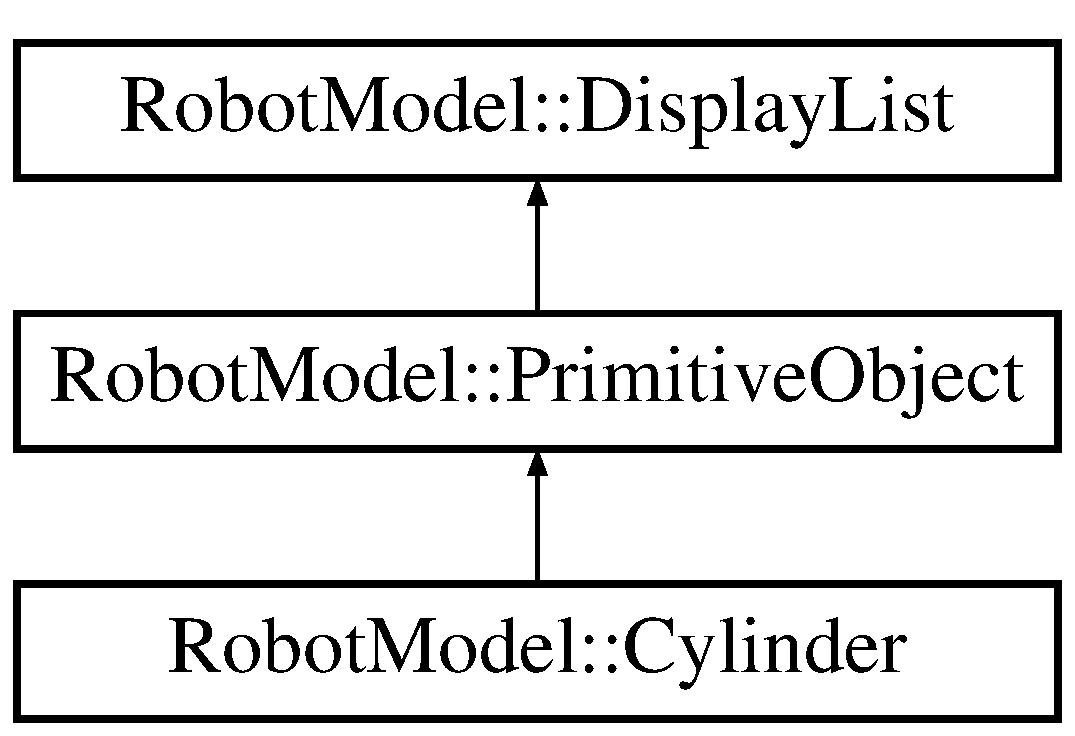
\includegraphics[height=2.35955cm]{class_robot_model_1_1_cylinder}
\end{center}
\end{figure}
\subsection*{Public Member Functions}
\begin{DoxyCompactItemize}
\item 
\hyperlink{class_robot_model_1_1_cylinder_aa738cca8df1e6a449662f33a814e67f8}{Cylinder} (qreal radius, qreal height, int lod=12)
\item 
\hyperlink{class_robot_model_1_1_cylinder_a05ab556f0ae3cd6e99d9d1f3caca80b3}{$\sim$Cylinder} ()
\item 
virtual void \hyperlink{class_robot_model_1_1_cylinder_a9f0361117d5f20344f543c9e20df1113}{makeDisplayList} ()
\item 
\hyperlink{class_robot_model_1_1_cylinder_a16c419bccd55814a38877eeb9b10f3c0}{Cylinder} (qreal radius, qreal height, int lod=12)
\item 
\hyperlink{class_robot_model_1_1_cylinder_a18a0f743261694851bdbc50339f423f2}{$\sim$Cylinder} ()
\item 
virtual void \hyperlink{class_robot_model_1_1_cylinder_a92e328e0a01f4fd787d73d4996d67b0a}{makeDisplayList} ()
\end{DoxyCompactItemize}


\subsection{Constructor \& Destructor Documentation}
\hypertarget{class_robot_model_1_1_cylinder_aa738cca8df1e6a449662f33a814e67f8}{
\index{RobotModel::Cylinder@{RobotModel::Cylinder}!Cylinder@{Cylinder}}
\index{Cylinder@{Cylinder}!RobotModel::Cylinder@{RobotModel::Cylinder}}
\subsubsection[{Cylinder}]{\setlength{\rightskip}{0pt plus 5cm}Cylinder::Cylinder (qreal {\em radius}, \/  qreal {\em height}, \/  int {\em lod} = {\ttfamily 12})}}
\label{class_robot_model_1_1_cylinder_aa738cca8df1e6a449662f33a814e67f8}
\hypertarget{class_robot_model_1_1_cylinder_a05ab556f0ae3cd6e99d9d1f3caca80b3}{
\index{RobotModel::Cylinder@{RobotModel::Cylinder}!$\sim$Cylinder@{$\sim$Cylinder}}
\index{$\sim$Cylinder@{$\sim$Cylinder}!RobotModel::Cylinder@{RobotModel::Cylinder}}
\subsubsection[{$\sim$Cylinder}]{\setlength{\rightskip}{0pt plus 5cm}Cylinder::$\sim$Cylinder ()}}
\label{class_robot_model_1_1_cylinder_a05ab556f0ae3cd6e99d9d1f3caca80b3}
\hypertarget{class_robot_model_1_1_cylinder_a16c419bccd55814a38877eeb9b10f3c0}{
\index{RobotModel::Cylinder@{RobotModel::Cylinder}!Cylinder@{Cylinder}}
\index{Cylinder@{Cylinder}!RobotModel::Cylinder@{RobotModel::Cylinder}}
\subsubsection[{Cylinder}]{\setlength{\rightskip}{0pt plus 5cm}RobotModel::Cylinder::Cylinder (qreal {\em radius}, \/  qreal {\em height}, \/  int {\em lod} = {\ttfamily 12})}}
\label{class_robot_model_1_1_cylinder_a16c419bccd55814a38877eeb9b10f3c0}
\hypertarget{class_robot_model_1_1_cylinder_a18a0f743261694851bdbc50339f423f2}{
\index{RobotModel::Cylinder@{RobotModel::Cylinder}!$\sim$Cylinder@{$\sim$Cylinder}}
\index{$\sim$Cylinder@{$\sim$Cylinder}!RobotModel::Cylinder@{RobotModel::Cylinder}}
\subsubsection[{$\sim$Cylinder}]{\setlength{\rightskip}{0pt plus 5cm}RobotModel::Cylinder::$\sim$Cylinder ()}}
\label{class_robot_model_1_1_cylinder_a18a0f743261694851bdbc50339f423f2}


\subsection{Member Function Documentation}
\hypertarget{class_robot_model_1_1_cylinder_a92e328e0a01f4fd787d73d4996d67b0a}{
\index{RobotModel::Cylinder@{RobotModel::Cylinder}!makeDisplayList@{makeDisplayList}}
\index{makeDisplayList@{makeDisplayList}!RobotModel::Cylinder@{RobotModel::Cylinder}}
\subsubsection[{makeDisplayList}]{\setlength{\rightskip}{0pt plus 5cm}virtual void RobotModel::Cylinder::makeDisplayList ()\hspace{0.3cm}{\ttfamily  \mbox{[}virtual\mbox{]}}}}
\label{class_robot_model_1_1_cylinder_a92e328e0a01f4fd787d73d4996d67b0a}


Implements \hyperlink{class_robot_model_1_1_display_list_a842de97924298c7363e50aebd69e5a50}{RobotModel::DisplayList}.\hypertarget{class_robot_model_1_1_cylinder_a9f0361117d5f20344f543c9e20df1113}{
\index{RobotModel::Cylinder@{RobotModel::Cylinder}!makeDisplayList@{makeDisplayList}}
\index{makeDisplayList@{makeDisplayList}!RobotModel::Cylinder@{RobotModel::Cylinder}}
\subsubsection[{makeDisplayList}]{\setlength{\rightskip}{0pt plus 5cm}void Cylinder::makeDisplayList ()\hspace{0.3cm}{\ttfamily  \mbox{[}virtual\mbox{]}}}}
\label{class_robot_model_1_1_cylinder_a9f0361117d5f20344f543c9e20df1113}


Implements \hyperlink{class_robot_model_1_1_display_list_a842de97924298c7363e50aebd69e5a50}{RobotModel::DisplayList}.

The documentation for this class was generated from the following files:\begin{DoxyCompactItemize}
\item 
/Users/kail/imClever/dev/virtualSkin/include/robotModel/\hyperlink{include_2robot_model_2cylinder_8h}{cylinder.h}\item 
/Users/kail/imClever/dev/virtualSkin/src/robotModel/\hyperlink{src_2robot_model_2cylinder_8h}{cylinder.h}\item 
/Users/kail/imClever/dev/virtualSkin/src/robotModel/\hyperlink{cylinder_8cpp}{cylinder.cpp}\end{DoxyCompactItemize}

\hypertarget{class_robot_model_1_1_display_list}{
\section{RobotModel::DisplayList Class Reference}
\label{class_robot_model_1_1_display_list}\index{RobotModel::DisplayList@{RobotModel::DisplayList}}
}


{\ttfamily \#include $<$displaylist.h$>$}Inheritance diagram for RobotModel::DisplayList::\begin{figure}[H]
\begin{center}
\leavevmode
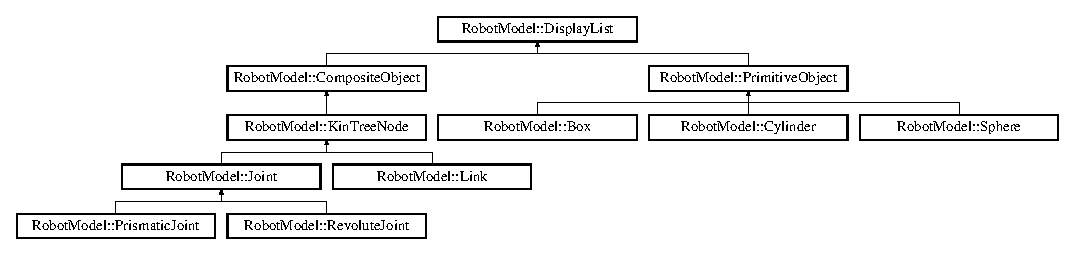
\includegraphics[height=2.97872cm]{class_robot_model_1_1_display_list}
\end{center}
\end{figure}
\subsection*{Public Member Functions}
\begin{DoxyCompactItemize}
\item 
\hyperlink{class_robot_model_1_1_display_list_a71d74802d0190f52c0c4ad7c6d5351f9}{DisplayList} ()
\item 
virtual \hyperlink{class_robot_model_1_1_display_list_a4c2105212d624723af920c798c1712cf}{$\sim$DisplayList} ()
\item 
virtual void \hyperlink{class_robot_model_1_1_display_list_a842de97924298c7363e50aebd69e5a50}{makeDisplayList} ()=0
\item 
virtual void \hyperlink{class_robot_model_1_1_display_list_a5f95e85c192a2bc8f06f18075e6fefd7}{render} ()
\item 
const \hyperlink{class_robot_model_1_1_displ_matrix}{DisplMatrix} \& \hyperlink{class_robot_model_1_1_display_list_a2e08e72148fc8bb77a693b769a16711a}{getT} ()
\item 
void \hyperlink{class_robot_model_1_1_display_list_a78c642f12487ea830475a0e860aeee38}{setDisplayListIdx} (int idx)
\item 
int \hyperlink{class_robot_model_1_1_display_list_a2c405729d9a5d904b9c292fd87c3be05}{displayListIdx} ()
\item 
void \hyperlink{class_robot_model_1_1_display_list_aab3355867d2a992c208f2173fc29e221}{setColliding} ()
\item 
void \hyperlink{class_robot_model_1_1_display_list_a7440037838409ae852e02183245b338d}{unSetColliding} ()
\item 
bool \hyperlink{class_robot_model_1_1_display_list_a32f1a046e32b479110977c5efec41cc3}{isColliding} () const 
\item 
virtual void \hyperlink{class_robot_model_1_1_display_list_a7d52ea010f54755bcb3bfae9e26dd0c2}{setCartesianRotation} (const QVector3D \&rot)
\item 
virtual void \hyperlink{class_robot_model_1_1_display_list_a023ba88eaac38b26dc9ea6a358467637}{cartesianRotate} (const QVector3D \&rot)
\item 
virtual void \hyperlink{class_robot_model_1_1_display_list_a56a652740c494995c0ff55d1a5fd896d}{setAxisAngleRotation} (const QVector3D \&axis, qreal angle)
\item 
virtual void \hyperlink{class_robot_model_1_1_display_list_a9a7084168997ac285ee1e9f4041a8d57}{axisAngleRotate} (const QVector3D \&axis, qreal angle)
\item 
virtual void \hyperlink{class_robot_model_1_1_display_list_abd15964fcf47dbfdcb06d89517871152}{specialRotate} (const QVector3D \&axis, qreal angle=0)
\item 
virtual void \hyperlink{class_robot_model_1_1_display_list_a6c9c1298e237ab25037ad9d7163b118c}{setTranslation} (const QVector3D \&trans)
\item 
virtual void \hyperlink{class_robot_model_1_1_display_list_a6eb574d1f9929d9e2141dbacdeeb1b6a}{translate} (const QVector3D \&trans)
\item 
\hyperlink{class_robot_model_1_1_display_list_a4791b78bf5b3ce2edb821fd9318b7117}{DisplayList} ()
\item 
virtual \hyperlink{class_robot_model_1_1_display_list_a4f3dfbc4d5278bf34ce02738a55af6b7}{$\sim$DisplayList} ()
\item 
virtual void \hyperlink{class_robot_model_1_1_display_list_a842de97924298c7363e50aebd69e5a50}{makeDisplayList} ()=0
\item 
virtual void \hyperlink{class_robot_model_1_1_display_list_ae1e118fc2339bdcaed1f39bd3b65ab32}{render} ()
\item 
const \hyperlink{class_robot_model_1_1_displ_matrix}{DisplMatrix} \& \hyperlink{class_robot_model_1_1_display_list_a2e08e72148fc8bb77a693b769a16711a}{getT} ()
\item 
void \hyperlink{class_robot_model_1_1_display_list_a78c642f12487ea830475a0e860aeee38}{setDisplayListIdx} (int idx)
\item 
int \hyperlink{class_robot_model_1_1_display_list_a2c405729d9a5d904b9c292fd87c3be05}{displayListIdx} ()
\item 
void \hyperlink{class_robot_model_1_1_display_list_aab3355867d2a992c208f2173fc29e221}{setColliding} ()
\item 
void \hyperlink{class_robot_model_1_1_display_list_a7440037838409ae852e02183245b338d}{unSetColliding} ()
\item 
bool \hyperlink{class_robot_model_1_1_display_list_a32f1a046e32b479110977c5efec41cc3}{isColliding} () const 
\item 
virtual void \hyperlink{class_robot_model_1_1_display_list_a7d52ea010f54755bcb3bfae9e26dd0c2}{setCartesianRotation} (const QVector3D \&rot)
\item 
virtual void \hyperlink{class_robot_model_1_1_display_list_a023ba88eaac38b26dc9ea6a358467637}{cartesianRotate} (const QVector3D \&rot)
\item 
virtual void \hyperlink{class_robot_model_1_1_display_list_a56a652740c494995c0ff55d1a5fd896d}{setAxisAngleRotation} (const QVector3D \&axis, qreal angle)
\item 
virtual void \hyperlink{class_robot_model_1_1_display_list_a9a7084168997ac285ee1e9f4041a8d57}{axisAngleRotate} (const QVector3D \&axis, qreal angle)
\item 
virtual void \hyperlink{class_robot_model_1_1_display_list_abd15964fcf47dbfdcb06d89517871152}{specialRotate} (const QVector3D \&axis, qreal angle=0)
\item 
virtual void \hyperlink{class_robot_model_1_1_display_list_a6c9c1298e237ab25037ad9d7163b118c}{setTranslation} (const QVector3D \&trans)
\item 
virtual void \hyperlink{class_robot_model_1_1_display_list_a6eb574d1f9929d9e2141dbacdeeb1b6a}{translate} (const QVector3D \&trans)
\end{DoxyCompactItemize}
\subsection*{Protected Attributes}
\begin{DoxyCompactItemize}
\item 
\hyperlink{class_robot_model_1_1_displ_matrix}{DisplMatrix} \hyperlink{class_robot_model_1_1_display_list_a9058babda6102fe41186f806990aa350}{T}
\end{DoxyCompactItemize}


\subsection{Constructor \& Destructor Documentation}
\hypertarget{class_robot_model_1_1_display_list_a71d74802d0190f52c0c4ad7c6d5351f9}{
\index{RobotModel::DisplayList@{RobotModel::DisplayList}!DisplayList@{DisplayList}}
\index{DisplayList@{DisplayList}!RobotModel::DisplayList@{RobotModel::DisplayList}}
\subsubsection[{DisplayList}]{\setlength{\rightskip}{0pt plus 5cm}DisplayList::DisplayList ()}}
\label{class_robot_model_1_1_display_list_a71d74802d0190f52c0c4ad7c6d5351f9}
\hypertarget{class_robot_model_1_1_display_list_a4c2105212d624723af920c798c1712cf}{
\index{RobotModel::DisplayList@{RobotModel::DisplayList}!$\sim$DisplayList@{$\sim$DisplayList}}
\index{$\sim$DisplayList@{$\sim$DisplayList}!RobotModel::DisplayList@{RobotModel::DisplayList}}
\subsubsection[{$\sim$DisplayList}]{\setlength{\rightskip}{0pt plus 5cm}DisplayList::$\sim$DisplayList ()\hspace{0.3cm}{\ttfamily  \mbox{[}virtual\mbox{]}}}}
\label{class_robot_model_1_1_display_list_a4c2105212d624723af920c798c1712cf}
\hypertarget{class_robot_model_1_1_display_list_a4791b78bf5b3ce2edb821fd9318b7117}{
\index{RobotModel::DisplayList@{RobotModel::DisplayList}!DisplayList@{DisplayList}}
\index{DisplayList@{DisplayList}!RobotModel::DisplayList@{RobotModel::DisplayList}}
\subsubsection[{DisplayList}]{\setlength{\rightskip}{0pt plus 5cm}RobotModel::DisplayList::DisplayList ()}}
\label{class_robot_model_1_1_display_list_a4791b78bf5b3ce2edb821fd9318b7117}
\hypertarget{class_robot_model_1_1_display_list_a4f3dfbc4d5278bf34ce02738a55af6b7}{
\index{RobotModel::DisplayList@{RobotModel::DisplayList}!$\sim$DisplayList@{$\sim$DisplayList}}
\index{$\sim$DisplayList@{$\sim$DisplayList}!RobotModel::DisplayList@{RobotModel::DisplayList}}
\subsubsection[{$\sim$DisplayList}]{\setlength{\rightskip}{0pt plus 5cm}virtual RobotModel::DisplayList::$\sim$DisplayList ()\hspace{0.3cm}{\ttfamily  \mbox{[}virtual\mbox{]}}}}
\label{class_robot_model_1_1_display_list_a4f3dfbc4d5278bf34ce02738a55af6b7}


\subsection{Member Function Documentation}
\hypertarget{class_robot_model_1_1_display_list_a9a7084168997ac285ee1e9f4041a8d57}{
\index{RobotModel::DisplayList@{RobotModel::DisplayList}!axisAngleRotate@{axisAngleRotate}}
\index{axisAngleRotate@{axisAngleRotate}!RobotModel::DisplayList@{RobotModel::DisplayList}}
\subsubsection[{axisAngleRotate}]{\setlength{\rightskip}{0pt plus 5cm}virtual void RobotModel::DisplayList::axisAngleRotate (const QVector3D \& {\em axis}, \/  qreal {\em angle})\hspace{0.3cm}{\ttfamily  \mbox{[}inline, virtual\mbox{]}}}}
\label{class_robot_model_1_1_display_list_a9a7084168997ac285ee1e9f4041a8d57}


Reimplemented in \hyperlink{class_robot_model_1_1_composite_object_a357f5ed3f49e0889df511271e468f866}{RobotModel::CompositeObject}, \hyperlink{class_robot_model_1_1_primitive_object_a97b449302680b96410ff7296c794f640}{RobotModel::PrimitiveObject}, \hyperlink{class_robot_model_1_1_composite_object_aa59e7af66ca1a0ced127d8f2b30c7a6d}{RobotModel::CompositeObject}, and \hyperlink{class_robot_model_1_1_primitive_object_ae57db819937782138821a30960a72aa0}{RobotModel::PrimitiveObject}.\hypertarget{class_robot_model_1_1_display_list_a9a7084168997ac285ee1e9f4041a8d57}{
\index{RobotModel::DisplayList@{RobotModel::DisplayList}!axisAngleRotate@{axisAngleRotate}}
\index{axisAngleRotate@{axisAngleRotate}!RobotModel::DisplayList@{RobotModel::DisplayList}}
\subsubsection[{axisAngleRotate}]{\setlength{\rightskip}{0pt plus 5cm}virtual void RobotModel::DisplayList::axisAngleRotate (const QVector3D \& {\em axis}, \/  qreal {\em angle})\hspace{0.3cm}{\ttfamily  \mbox{[}inline, virtual\mbox{]}}}}
\label{class_robot_model_1_1_display_list_a9a7084168997ac285ee1e9f4041a8d57}


Reimplemented in \hyperlink{class_robot_model_1_1_composite_object_a357f5ed3f49e0889df511271e468f866}{RobotModel::CompositeObject}, \hyperlink{class_robot_model_1_1_primitive_object_a97b449302680b96410ff7296c794f640}{RobotModel::PrimitiveObject}, \hyperlink{class_robot_model_1_1_composite_object_aa59e7af66ca1a0ced127d8f2b30c7a6d}{RobotModel::CompositeObject}, and \hyperlink{class_robot_model_1_1_primitive_object_ae57db819937782138821a30960a72aa0}{RobotModel::PrimitiveObject}.\hypertarget{class_robot_model_1_1_display_list_a023ba88eaac38b26dc9ea6a358467637}{
\index{RobotModel::DisplayList@{RobotModel::DisplayList}!cartesianRotate@{cartesianRotate}}
\index{cartesianRotate@{cartesianRotate}!RobotModel::DisplayList@{RobotModel::DisplayList}}
\subsubsection[{cartesianRotate}]{\setlength{\rightskip}{0pt plus 5cm}virtual void RobotModel::DisplayList::cartesianRotate (const QVector3D \& {\em rot})\hspace{0.3cm}{\ttfamily  \mbox{[}inline, virtual\mbox{]}}}}
\label{class_robot_model_1_1_display_list_a023ba88eaac38b26dc9ea6a358467637}


Reimplemented in \hyperlink{class_robot_model_1_1_composite_object_adadc29cccbba9cb615eaf0ad2fbdd337}{RobotModel::CompositeObject}, \hyperlink{class_robot_model_1_1_primitive_object_a69c30287deb6549fbde68d1ba37424a8}{RobotModel::PrimitiveObject}, \hyperlink{class_robot_model_1_1_composite_object_a7c46e273df7d93cb51b9e16158469509}{RobotModel::CompositeObject}, and \hyperlink{class_robot_model_1_1_primitive_object_aa490f6642a6a02d48cf8ed9cd49a47f7}{RobotModel::PrimitiveObject}.\hypertarget{class_robot_model_1_1_display_list_a023ba88eaac38b26dc9ea6a358467637}{
\index{RobotModel::DisplayList@{RobotModel::DisplayList}!cartesianRotate@{cartesianRotate}}
\index{cartesianRotate@{cartesianRotate}!RobotModel::DisplayList@{RobotModel::DisplayList}}
\subsubsection[{cartesianRotate}]{\setlength{\rightskip}{0pt plus 5cm}virtual void RobotModel::DisplayList::cartesianRotate (const QVector3D \& {\em rot})\hspace{0.3cm}{\ttfamily  \mbox{[}inline, virtual\mbox{]}}}}
\label{class_robot_model_1_1_display_list_a023ba88eaac38b26dc9ea6a358467637}


Reimplemented in \hyperlink{class_robot_model_1_1_composite_object_adadc29cccbba9cb615eaf0ad2fbdd337}{RobotModel::CompositeObject}, \hyperlink{class_robot_model_1_1_primitive_object_a69c30287deb6549fbde68d1ba37424a8}{RobotModel::PrimitiveObject}, \hyperlink{class_robot_model_1_1_composite_object_a7c46e273df7d93cb51b9e16158469509}{RobotModel::CompositeObject}, and \hyperlink{class_robot_model_1_1_primitive_object_aa490f6642a6a02d48cf8ed9cd49a47f7}{RobotModel::PrimitiveObject}.\hypertarget{class_robot_model_1_1_display_list_a2c405729d9a5d904b9c292fd87c3be05}{
\index{RobotModel::DisplayList@{RobotModel::DisplayList}!displayListIdx@{displayListIdx}}
\index{displayListIdx@{displayListIdx}!RobotModel::DisplayList@{RobotModel::DisplayList}}
\subsubsection[{displayListIdx}]{\setlength{\rightskip}{0pt plus 5cm}int RobotModel::DisplayList::displayListIdx ()\hspace{0.3cm}{\ttfamily  \mbox{[}inline\mbox{]}}}}
\label{class_robot_model_1_1_display_list_a2c405729d9a5d904b9c292fd87c3be05}
\hypertarget{class_robot_model_1_1_display_list_a2c405729d9a5d904b9c292fd87c3be05}{
\index{RobotModel::DisplayList@{RobotModel::DisplayList}!displayListIdx@{displayListIdx}}
\index{displayListIdx@{displayListIdx}!RobotModel::DisplayList@{RobotModel::DisplayList}}
\subsubsection[{displayListIdx}]{\setlength{\rightskip}{0pt plus 5cm}int RobotModel::DisplayList::displayListIdx ()\hspace{0.3cm}{\ttfamily  \mbox{[}inline\mbox{]}}}}
\label{class_robot_model_1_1_display_list_a2c405729d9a5d904b9c292fd87c3be05}
\hypertarget{class_robot_model_1_1_display_list_a2e08e72148fc8bb77a693b769a16711a}{
\index{RobotModel::DisplayList@{RobotModel::DisplayList}!getT@{getT}}
\index{getT@{getT}!RobotModel::DisplayList@{RobotModel::DisplayList}}
\subsubsection[{getT}]{\setlength{\rightskip}{0pt plus 5cm}const {\bf DisplMatrix}\& RobotModel::DisplayList::getT ()\hspace{0.3cm}{\ttfamily  \mbox{[}inline\mbox{]}}}}
\label{class_robot_model_1_1_display_list_a2e08e72148fc8bb77a693b769a16711a}
\hypertarget{class_robot_model_1_1_display_list_a2e08e72148fc8bb77a693b769a16711a}{
\index{RobotModel::DisplayList@{RobotModel::DisplayList}!getT@{getT}}
\index{getT@{getT}!RobotModel::DisplayList@{RobotModel::DisplayList}}
\subsubsection[{getT}]{\setlength{\rightskip}{0pt plus 5cm}const {\bf DisplMatrix}\& RobotModel::DisplayList::getT ()\hspace{0.3cm}{\ttfamily  \mbox{[}inline\mbox{]}}}}
\label{class_robot_model_1_1_display_list_a2e08e72148fc8bb77a693b769a16711a}
\hypertarget{class_robot_model_1_1_display_list_a32f1a046e32b479110977c5efec41cc3}{
\index{RobotModel::DisplayList@{RobotModel::DisplayList}!isColliding@{isColliding}}
\index{isColliding@{isColliding}!RobotModel::DisplayList@{RobotModel::DisplayList}}
\subsubsection[{isColliding}]{\setlength{\rightskip}{0pt plus 5cm}bool RobotModel::DisplayList::isColliding () const\hspace{0.3cm}{\ttfamily  \mbox{[}inline\mbox{]}}}}
\label{class_robot_model_1_1_display_list_a32f1a046e32b479110977c5efec41cc3}
\hypertarget{class_robot_model_1_1_display_list_a32f1a046e32b479110977c5efec41cc3}{
\index{RobotModel::DisplayList@{RobotModel::DisplayList}!isColliding@{isColliding}}
\index{isColliding@{isColliding}!RobotModel::DisplayList@{RobotModel::DisplayList}}
\subsubsection[{isColliding}]{\setlength{\rightskip}{0pt plus 5cm}bool RobotModel::DisplayList::isColliding () const\hspace{0.3cm}{\ttfamily  \mbox{[}inline\mbox{]}}}}
\label{class_robot_model_1_1_display_list_a32f1a046e32b479110977c5efec41cc3}
\hypertarget{class_robot_model_1_1_display_list_a842de97924298c7363e50aebd69e5a50}{
\index{RobotModel::DisplayList@{RobotModel::DisplayList}!makeDisplayList@{makeDisplayList}}
\index{makeDisplayList@{makeDisplayList}!RobotModel::DisplayList@{RobotModel::DisplayList}}
\subsubsection[{makeDisplayList}]{\setlength{\rightskip}{0pt plus 5cm}virtual void RobotModel::DisplayList::makeDisplayList ()\hspace{0.3cm}{\ttfamily  \mbox{[}pure virtual\mbox{]}}}}
\label{class_robot_model_1_1_display_list_a842de97924298c7363e50aebd69e5a50}


Implemented in \hyperlink{class_robot_model_1_1_box_a29420d81c8b3622c95a1976593e2cc4b}{RobotModel::Box}, \hyperlink{class_robot_model_1_1_cylinder_a9f0361117d5f20344f543c9e20df1113}{RobotModel::Cylinder}, \hyperlink{class_robot_model_1_1_composite_object_a5aa475cb09f0e9b9089a941848f9e189}{RobotModel::CompositeObject}, \hyperlink{class_robot_model_1_1_sphere_a838b5ae4f743aabe24a255dd61d2843c}{RobotModel::Sphere}, \hyperlink{class_robot_model_1_1_box_a9499dafbda230821b419e3f578316d91}{RobotModel::Box}, \hyperlink{class_robot_model_1_1_cylinder_a92e328e0a01f4fd787d73d4996d67b0a}{RobotModel::Cylinder}, \hyperlink{class_robot_model_1_1_composite_object_a780659c8a3d7803bf61ac55227ea0e3f}{RobotModel::CompositeObject}, and \hyperlink{class_robot_model_1_1_sphere_a0f338501410a9d8e220ff20ce073d244}{RobotModel::Sphere}.\hypertarget{class_robot_model_1_1_display_list_a842de97924298c7363e50aebd69e5a50}{
\index{RobotModel::DisplayList@{RobotModel::DisplayList}!makeDisplayList@{makeDisplayList}}
\index{makeDisplayList@{makeDisplayList}!RobotModel::DisplayList@{RobotModel::DisplayList}}
\subsubsection[{makeDisplayList}]{\setlength{\rightskip}{0pt plus 5cm}virtual void RobotModel::DisplayList::makeDisplayList ()\hspace{0.3cm}{\ttfamily  \mbox{[}pure virtual\mbox{]}}}}
\label{class_robot_model_1_1_display_list_a842de97924298c7363e50aebd69e5a50}


Implemented in \hyperlink{class_robot_model_1_1_box_a29420d81c8b3622c95a1976593e2cc4b}{RobotModel::Box}, \hyperlink{class_robot_model_1_1_cylinder_a9f0361117d5f20344f543c9e20df1113}{RobotModel::Cylinder}, \hyperlink{class_robot_model_1_1_composite_object_a5aa475cb09f0e9b9089a941848f9e189}{RobotModel::CompositeObject}, \hyperlink{class_robot_model_1_1_sphere_a838b5ae4f743aabe24a255dd61d2843c}{RobotModel::Sphere}, \hyperlink{class_robot_model_1_1_box_a9499dafbda230821b419e3f578316d91}{RobotModel::Box}, \hyperlink{class_robot_model_1_1_cylinder_a92e328e0a01f4fd787d73d4996d67b0a}{RobotModel::Cylinder}, \hyperlink{class_robot_model_1_1_composite_object_a780659c8a3d7803bf61ac55227ea0e3f}{RobotModel::CompositeObject}, and \hyperlink{class_robot_model_1_1_sphere_a0f338501410a9d8e220ff20ce073d244}{RobotModel::Sphere}.\hypertarget{class_robot_model_1_1_display_list_ae1e118fc2339bdcaed1f39bd3b65ab32}{
\index{RobotModel::DisplayList@{RobotModel::DisplayList}!render@{render}}
\index{render@{render}!RobotModel::DisplayList@{RobotModel::DisplayList}}
\subsubsection[{render}]{\setlength{\rightskip}{0pt plus 5cm}virtual void RobotModel::DisplayList::render ()\hspace{0.3cm}{\ttfamily  \mbox{[}virtual\mbox{]}}}}
\label{class_robot_model_1_1_display_list_ae1e118fc2339bdcaed1f39bd3b65ab32}


Reimplemented in \hyperlink{class_robot_model_1_1_kin_tree_node_a85f4364980f9144471b9d92e175c539e}{RobotModel::KinTreeNode}, \hyperlink{class_robot_model_1_1_composite_object_aee43da74b22f6272736844effe7a1dd6}{RobotModel::CompositeObject}, \hyperlink{class_robot_model_1_1_kin_tree_node_a7ccf98213f418d0e5efa4f699d898f2d}{RobotModel::KinTreeNode}, and \hyperlink{class_robot_model_1_1_composite_object_a580d00dd3a303972d34183c07625aed7}{RobotModel::CompositeObject}.\hypertarget{class_robot_model_1_1_display_list_a5f95e85c192a2bc8f06f18075e6fefd7}{
\index{RobotModel::DisplayList@{RobotModel::DisplayList}!render@{render}}
\index{render@{render}!RobotModel::DisplayList@{RobotModel::DisplayList}}
\subsubsection[{render}]{\setlength{\rightskip}{0pt plus 5cm}void DisplayList::render ()\hspace{0.3cm}{\ttfamily  \mbox{[}virtual\mbox{]}}}}
\label{class_robot_model_1_1_display_list_a5f95e85c192a2bc8f06f18075e6fefd7}


Reimplemented in \hyperlink{class_robot_model_1_1_kin_tree_node_a85f4364980f9144471b9d92e175c539e}{RobotModel::KinTreeNode}, \hyperlink{class_robot_model_1_1_composite_object_aee43da74b22f6272736844effe7a1dd6}{RobotModel::CompositeObject}, \hyperlink{class_robot_model_1_1_kin_tree_node_a7ccf98213f418d0e5efa4f699d898f2d}{RobotModel::KinTreeNode}, and \hyperlink{class_robot_model_1_1_composite_object_a580d00dd3a303972d34183c07625aed7}{RobotModel::CompositeObject}.\hypertarget{class_robot_model_1_1_display_list_a56a652740c494995c0ff55d1a5fd896d}{
\index{RobotModel::DisplayList@{RobotModel::DisplayList}!setAxisAngleRotation@{setAxisAngleRotation}}
\index{setAxisAngleRotation@{setAxisAngleRotation}!RobotModel::DisplayList@{RobotModel::DisplayList}}
\subsubsection[{setAxisAngleRotation}]{\setlength{\rightskip}{0pt plus 5cm}virtual void RobotModel::DisplayList::setAxisAngleRotation (const QVector3D \& {\em axis}, \/  qreal {\em angle})\hspace{0.3cm}{\ttfamily  \mbox{[}inline, virtual\mbox{]}}}}
\label{class_robot_model_1_1_display_list_a56a652740c494995c0ff55d1a5fd896d}


Reimplemented in \hyperlink{class_robot_model_1_1_composite_object_a43f99ed52def7114d310e29fc6db83f3}{RobotModel::CompositeObject}, \hyperlink{class_robot_model_1_1_primitive_object_a3ae3782ae64f5fc07f4d18646e04ed21}{RobotModel::PrimitiveObject}, \hyperlink{class_robot_model_1_1_composite_object_a718690c002e0f74b430a75a9c4dfdf85}{RobotModel::CompositeObject}, and \hyperlink{class_robot_model_1_1_primitive_object_a4a91537e10478b31fb8a025c0faac770}{RobotModel::PrimitiveObject}.\hypertarget{class_robot_model_1_1_display_list_a56a652740c494995c0ff55d1a5fd896d}{
\index{RobotModel::DisplayList@{RobotModel::DisplayList}!setAxisAngleRotation@{setAxisAngleRotation}}
\index{setAxisAngleRotation@{setAxisAngleRotation}!RobotModel::DisplayList@{RobotModel::DisplayList}}
\subsubsection[{setAxisAngleRotation}]{\setlength{\rightskip}{0pt plus 5cm}virtual void RobotModel::DisplayList::setAxisAngleRotation (const QVector3D \& {\em axis}, \/  qreal {\em angle})\hspace{0.3cm}{\ttfamily  \mbox{[}inline, virtual\mbox{]}}}}
\label{class_robot_model_1_1_display_list_a56a652740c494995c0ff55d1a5fd896d}


Reimplemented in \hyperlink{class_robot_model_1_1_composite_object_a43f99ed52def7114d310e29fc6db83f3}{RobotModel::CompositeObject}, \hyperlink{class_robot_model_1_1_primitive_object_a3ae3782ae64f5fc07f4d18646e04ed21}{RobotModel::PrimitiveObject}, \hyperlink{class_robot_model_1_1_composite_object_a718690c002e0f74b430a75a9c4dfdf85}{RobotModel::CompositeObject}, and \hyperlink{class_robot_model_1_1_primitive_object_a4a91537e10478b31fb8a025c0faac770}{RobotModel::PrimitiveObject}.\hypertarget{class_robot_model_1_1_display_list_a7d52ea010f54755bcb3bfae9e26dd0c2}{
\index{RobotModel::DisplayList@{RobotModel::DisplayList}!setCartesianRotation@{setCartesianRotation}}
\index{setCartesianRotation@{setCartesianRotation}!RobotModel::DisplayList@{RobotModel::DisplayList}}
\subsubsection[{setCartesianRotation}]{\setlength{\rightskip}{0pt plus 5cm}virtual void RobotModel::DisplayList::setCartesianRotation (const QVector3D \& {\em rot})\hspace{0.3cm}{\ttfamily  \mbox{[}inline, virtual\mbox{]}}}}
\label{class_robot_model_1_1_display_list_a7d52ea010f54755bcb3bfae9e26dd0c2}


Reimplemented in \hyperlink{class_robot_model_1_1_composite_object_a12e8961ebc63d8a253d915b29b356162}{RobotModel::CompositeObject}, \hyperlink{class_robot_model_1_1_primitive_object_a0a7cfefb126e4f37c208c516f8ffd9bb}{RobotModel::PrimitiveObject}, \hyperlink{class_robot_model_1_1_composite_object_a2e4886f283bbf8741c41a066241a1e55}{RobotModel::CompositeObject}, and \hyperlink{class_robot_model_1_1_primitive_object_afa2afdbe412aadfe4d7bb951e4d7b8fa}{RobotModel::PrimitiveObject}.\hypertarget{class_robot_model_1_1_display_list_a7d52ea010f54755bcb3bfae9e26dd0c2}{
\index{RobotModel::DisplayList@{RobotModel::DisplayList}!setCartesianRotation@{setCartesianRotation}}
\index{setCartesianRotation@{setCartesianRotation}!RobotModel::DisplayList@{RobotModel::DisplayList}}
\subsubsection[{setCartesianRotation}]{\setlength{\rightskip}{0pt plus 5cm}virtual void RobotModel::DisplayList::setCartesianRotation (const QVector3D \& {\em rot})\hspace{0.3cm}{\ttfamily  \mbox{[}inline, virtual\mbox{]}}}}
\label{class_robot_model_1_1_display_list_a7d52ea010f54755bcb3bfae9e26dd0c2}


Reimplemented in \hyperlink{class_robot_model_1_1_composite_object_a12e8961ebc63d8a253d915b29b356162}{RobotModel::CompositeObject}, \hyperlink{class_robot_model_1_1_primitive_object_a0a7cfefb126e4f37c208c516f8ffd9bb}{RobotModel::PrimitiveObject}, \hyperlink{class_robot_model_1_1_composite_object_a2e4886f283bbf8741c41a066241a1e55}{RobotModel::CompositeObject}, and \hyperlink{class_robot_model_1_1_primitive_object_afa2afdbe412aadfe4d7bb951e4d7b8fa}{RobotModel::PrimitiveObject}.\hypertarget{class_robot_model_1_1_display_list_aab3355867d2a992c208f2173fc29e221}{
\index{RobotModel::DisplayList@{RobotModel::DisplayList}!setColliding@{setColliding}}
\index{setColliding@{setColliding}!RobotModel::DisplayList@{RobotModel::DisplayList}}
\subsubsection[{setColliding}]{\setlength{\rightskip}{0pt plus 5cm}void RobotModel::DisplayList::setColliding ()\hspace{0.3cm}{\ttfamily  \mbox{[}inline\mbox{]}}}}
\label{class_robot_model_1_1_display_list_aab3355867d2a992c208f2173fc29e221}
\hypertarget{class_robot_model_1_1_display_list_aab3355867d2a992c208f2173fc29e221}{
\index{RobotModel::DisplayList@{RobotModel::DisplayList}!setColliding@{setColliding}}
\index{setColliding@{setColliding}!RobotModel::DisplayList@{RobotModel::DisplayList}}
\subsubsection[{setColliding}]{\setlength{\rightskip}{0pt plus 5cm}void RobotModel::DisplayList::setColliding ()\hspace{0.3cm}{\ttfamily  \mbox{[}inline\mbox{]}}}}
\label{class_robot_model_1_1_display_list_aab3355867d2a992c208f2173fc29e221}
\hypertarget{class_robot_model_1_1_display_list_a78c642f12487ea830475a0e860aeee38}{
\index{RobotModel::DisplayList@{RobotModel::DisplayList}!setDisplayListIdx@{setDisplayListIdx}}
\index{setDisplayListIdx@{setDisplayListIdx}!RobotModel::DisplayList@{RobotModel::DisplayList}}
\subsubsection[{setDisplayListIdx}]{\setlength{\rightskip}{0pt plus 5cm}void RobotModel::DisplayList::setDisplayListIdx (int {\em idx})\hspace{0.3cm}{\ttfamily  \mbox{[}inline\mbox{]}}}}
\label{class_robot_model_1_1_display_list_a78c642f12487ea830475a0e860aeee38}
\hypertarget{class_robot_model_1_1_display_list_a78c642f12487ea830475a0e860aeee38}{
\index{RobotModel::DisplayList@{RobotModel::DisplayList}!setDisplayListIdx@{setDisplayListIdx}}
\index{setDisplayListIdx@{setDisplayListIdx}!RobotModel::DisplayList@{RobotModel::DisplayList}}
\subsubsection[{setDisplayListIdx}]{\setlength{\rightskip}{0pt plus 5cm}void RobotModel::DisplayList::setDisplayListIdx (int {\em idx})\hspace{0.3cm}{\ttfamily  \mbox{[}inline\mbox{]}}}}
\label{class_robot_model_1_1_display_list_a78c642f12487ea830475a0e860aeee38}
\hypertarget{class_robot_model_1_1_display_list_a6c9c1298e237ab25037ad9d7163b118c}{
\index{RobotModel::DisplayList@{RobotModel::DisplayList}!setTranslation@{setTranslation}}
\index{setTranslation@{setTranslation}!RobotModel::DisplayList@{RobotModel::DisplayList}}
\subsubsection[{setTranslation}]{\setlength{\rightskip}{0pt plus 5cm}virtual void RobotModel::DisplayList::setTranslation (const QVector3D \& {\em trans})\hspace{0.3cm}{\ttfamily  \mbox{[}inline, virtual\mbox{]}}}}
\label{class_robot_model_1_1_display_list_a6c9c1298e237ab25037ad9d7163b118c}


Reimplemented in \hyperlink{class_robot_model_1_1_composite_object_ae925e59246174c9d3b74d459b32835e3}{RobotModel::CompositeObject}, \hyperlink{class_robot_model_1_1_primitive_object_ae6c417003b52df18a52711031e95c44a}{RobotModel::PrimitiveObject}, \hyperlink{class_robot_model_1_1_composite_object_a6a24e273234d2919c48d36182c409ffd}{RobotModel::CompositeObject}, and \hyperlink{class_robot_model_1_1_primitive_object_a58f3d8655dd442ee1032f3582027604a}{RobotModel::PrimitiveObject}.\hypertarget{class_robot_model_1_1_display_list_a6c9c1298e237ab25037ad9d7163b118c}{
\index{RobotModel::DisplayList@{RobotModel::DisplayList}!setTranslation@{setTranslation}}
\index{setTranslation@{setTranslation}!RobotModel::DisplayList@{RobotModel::DisplayList}}
\subsubsection[{setTranslation}]{\setlength{\rightskip}{0pt plus 5cm}virtual void RobotModel::DisplayList::setTranslation (const QVector3D \& {\em trans})\hspace{0.3cm}{\ttfamily  \mbox{[}inline, virtual\mbox{]}}}}
\label{class_robot_model_1_1_display_list_a6c9c1298e237ab25037ad9d7163b118c}


Reimplemented in \hyperlink{class_robot_model_1_1_composite_object_ae925e59246174c9d3b74d459b32835e3}{RobotModel::CompositeObject}, \hyperlink{class_robot_model_1_1_primitive_object_ae6c417003b52df18a52711031e95c44a}{RobotModel::PrimitiveObject}, \hyperlink{class_robot_model_1_1_composite_object_a6a24e273234d2919c48d36182c409ffd}{RobotModel::CompositeObject}, and \hyperlink{class_robot_model_1_1_primitive_object_a58f3d8655dd442ee1032f3582027604a}{RobotModel::PrimitiveObject}.\hypertarget{class_robot_model_1_1_display_list_abd15964fcf47dbfdcb06d89517871152}{
\index{RobotModel::DisplayList@{RobotModel::DisplayList}!specialRotate@{specialRotate}}
\index{specialRotate@{specialRotate}!RobotModel::DisplayList@{RobotModel::DisplayList}}
\subsubsection[{specialRotate}]{\setlength{\rightskip}{0pt plus 5cm}virtual void RobotModel::DisplayList::specialRotate (const QVector3D \& {\em axis}, \/  qreal {\em angle} = {\ttfamily 0})\hspace{0.3cm}{\ttfamily  \mbox{[}inline, virtual\mbox{]}}}}
\label{class_robot_model_1_1_display_list_abd15964fcf47dbfdcb06d89517871152}


Reimplemented in \hyperlink{class_robot_model_1_1_composite_object_ad44b9c1759209367754dafd77c984d6f}{RobotModel::CompositeObject}, \hyperlink{class_robot_model_1_1_primitive_object_a07ece283ed8f0f0e3cdf6f36ac7b34dd}{RobotModel::PrimitiveObject}, \hyperlink{class_robot_model_1_1_composite_object_a3e9c7e78a85dc50e5327d5b5c99cc67e}{RobotModel::CompositeObject}, and \hyperlink{class_robot_model_1_1_primitive_object_a33c01b56d7daf2e1d94419f25b9fa902}{RobotModel::PrimitiveObject}.\hypertarget{class_robot_model_1_1_display_list_abd15964fcf47dbfdcb06d89517871152}{
\index{RobotModel::DisplayList@{RobotModel::DisplayList}!specialRotate@{specialRotate}}
\index{specialRotate@{specialRotate}!RobotModel::DisplayList@{RobotModel::DisplayList}}
\subsubsection[{specialRotate}]{\setlength{\rightskip}{0pt plus 5cm}virtual void RobotModel::DisplayList::specialRotate (const QVector3D \& {\em axis}, \/  qreal {\em angle} = {\ttfamily 0})\hspace{0.3cm}{\ttfamily  \mbox{[}inline, virtual\mbox{]}}}}
\label{class_robot_model_1_1_display_list_abd15964fcf47dbfdcb06d89517871152}


Reimplemented in \hyperlink{class_robot_model_1_1_composite_object_ad44b9c1759209367754dafd77c984d6f}{RobotModel::CompositeObject}, \hyperlink{class_robot_model_1_1_primitive_object_a07ece283ed8f0f0e3cdf6f36ac7b34dd}{RobotModel::PrimitiveObject}, \hyperlink{class_robot_model_1_1_composite_object_a3e9c7e78a85dc50e5327d5b5c99cc67e}{RobotModel::CompositeObject}, and \hyperlink{class_robot_model_1_1_primitive_object_a33c01b56d7daf2e1d94419f25b9fa902}{RobotModel::PrimitiveObject}.\hypertarget{class_robot_model_1_1_display_list_a6eb574d1f9929d9e2141dbacdeeb1b6a}{
\index{RobotModel::DisplayList@{RobotModel::DisplayList}!translate@{translate}}
\index{translate@{translate}!RobotModel::DisplayList@{RobotModel::DisplayList}}
\subsubsection[{translate}]{\setlength{\rightskip}{0pt plus 5cm}virtual void RobotModel::DisplayList::translate (const QVector3D \& {\em trans})\hspace{0.3cm}{\ttfamily  \mbox{[}inline, virtual\mbox{]}}}}
\label{class_robot_model_1_1_display_list_a6eb574d1f9929d9e2141dbacdeeb1b6a}


Reimplemented in \hyperlink{class_robot_model_1_1_composite_object_afd942b7fa3b18bcc01c3fba417a6c027}{RobotModel::CompositeObject}, \hyperlink{class_robot_model_1_1_primitive_object_ae41a1dcacd77b59c44409a77b0183a77}{RobotModel::PrimitiveObject}, \hyperlink{class_robot_model_1_1_composite_object_a7704da6de6211738327170423c1a3d83}{RobotModel::CompositeObject}, and \hyperlink{class_robot_model_1_1_primitive_object_aeddf2c45f6a3d60f2566e58728cc2a96}{RobotModel::PrimitiveObject}.\hypertarget{class_robot_model_1_1_display_list_a6eb574d1f9929d9e2141dbacdeeb1b6a}{
\index{RobotModel::DisplayList@{RobotModel::DisplayList}!translate@{translate}}
\index{translate@{translate}!RobotModel::DisplayList@{RobotModel::DisplayList}}
\subsubsection[{translate}]{\setlength{\rightskip}{0pt plus 5cm}virtual void RobotModel::DisplayList::translate (const QVector3D \& {\em trans})\hspace{0.3cm}{\ttfamily  \mbox{[}inline, virtual\mbox{]}}}}
\label{class_robot_model_1_1_display_list_a6eb574d1f9929d9e2141dbacdeeb1b6a}


Reimplemented in \hyperlink{class_robot_model_1_1_composite_object_afd942b7fa3b18bcc01c3fba417a6c027}{RobotModel::CompositeObject}, \hyperlink{class_robot_model_1_1_primitive_object_ae41a1dcacd77b59c44409a77b0183a77}{RobotModel::PrimitiveObject}, \hyperlink{class_robot_model_1_1_composite_object_a7704da6de6211738327170423c1a3d83}{RobotModel::CompositeObject}, and \hyperlink{class_robot_model_1_1_primitive_object_aeddf2c45f6a3d60f2566e58728cc2a96}{RobotModel::PrimitiveObject}.\hypertarget{class_robot_model_1_1_display_list_a7440037838409ae852e02183245b338d}{
\index{RobotModel::DisplayList@{RobotModel::DisplayList}!unSetColliding@{unSetColliding}}
\index{unSetColliding@{unSetColliding}!RobotModel::DisplayList@{RobotModel::DisplayList}}
\subsubsection[{unSetColliding}]{\setlength{\rightskip}{0pt plus 5cm}void RobotModel::DisplayList::unSetColliding ()\hspace{0.3cm}{\ttfamily  \mbox{[}inline\mbox{]}}}}
\label{class_robot_model_1_1_display_list_a7440037838409ae852e02183245b338d}
\hypertarget{class_robot_model_1_1_display_list_a7440037838409ae852e02183245b338d}{
\index{RobotModel::DisplayList@{RobotModel::DisplayList}!unSetColliding@{unSetColliding}}
\index{unSetColliding@{unSetColliding}!RobotModel::DisplayList@{RobotModel::DisplayList}}
\subsubsection[{unSetColliding}]{\setlength{\rightskip}{0pt plus 5cm}void RobotModel::DisplayList::unSetColliding ()\hspace{0.3cm}{\ttfamily  \mbox{[}inline\mbox{]}}}}
\label{class_robot_model_1_1_display_list_a7440037838409ae852e02183245b338d}


\subsection{Member Data Documentation}
\hypertarget{class_robot_model_1_1_display_list_a9058babda6102fe41186f806990aa350}{
\index{RobotModel::DisplayList@{RobotModel::DisplayList}!T@{T}}
\index{T@{T}!RobotModel::DisplayList@{RobotModel::DisplayList}}
\subsubsection[{T}]{\setlength{\rightskip}{0pt plus 5cm}{\bf DisplMatrix} {\bf RobotModel::DisplayList::T}\hspace{0.3cm}{\ttfamily  \mbox{[}protected\mbox{]}}}}
\label{class_robot_model_1_1_display_list_a9058babda6102fe41186f806990aa350}


The documentation for this class was generated from the following files:\begin{DoxyCompactItemize}
\item 
/Users/kail/imClever/dev/virtualSkin/include/robotModel/\hyperlink{include_2robot_model_2displaylist_8h}{displaylist.h}\item 
/Users/kail/imClever/dev/virtualSkin/src/robotModel/\hyperlink{src_2robot_model_2displaylist_8h}{displaylist.h}\item 
/Users/kail/imClever/dev/virtualSkin/src/robotModel/\hyperlink{displaylist_8cpp}{displaylist.cpp}\end{DoxyCompactItemize}

\hypertarget{class_robot_model_1_1_displ_matrix}{
\section{RobotModel::DisplMatrix Class Reference}
\label{class_robot_model_1_1_displ_matrix}\index{RobotModel::DisplMatrix@{RobotModel::DisplMatrix}}
}


{\ttfamily \#include $<$displmatrix.h$>$}\subsection*{Public Member Functions}
\begin{DoxyCompactItemize}
\item 
\hyperlink{class_robot_model_1_1_displ_matrix_a97463ac04605597575600274a23109de}{DisplMatrix} ()
\item 
\hyperlink{class_robot_model_1_1_displ_matrix_a6934f8d81e8e5b9c8dbcc1d6fd68c560}{DisplMatrix} (const QMatrix4x4 \&m)
\item 
void \hyperlink{class_robot_model_1_1_displ_matrix_a9ea9b65326be614baea1ea86a2a1b258}{setTranslation} (const QVector3D \&trans)
\item 
void \hyperlink{class_robot_model_1_1_displ_matrix_ae9aa3671b52f8300ac2f11648fa1fddf}{translate} (const QVector3D \&trans)
\item 
void \hyperlink{class_robot_model_1_1_displ_matrix_a8654f5029974e0154c3c46ec2bb3dbe3}{setCartesianRotation} (const QVector3D \&rot)
\item 
void \hyperlink{class_robot_model_1_1_displ_matrix_a337c49b52435255a7f36966c7047f6ff}{cartesianRotate} (const QVector3D \&rot)
\item 
void \hyperlink{class_robot_model_1_1_displ_matrix_ab976907c6be66c0aee20a24991ce4159}{setAxisAngleRotation} (const QVector3D \&axis, qreal angle)
\item 
void \hyperlink{class_robot_model_1_1_displ_matrix_aaf591b95247e1a80332ba0033427af7e}{axisAngleRotate} (const QVector3D \&axis, qreal angle)
\item 
void \hyperlink{class_robot_model_1_1_displ_matrix_ac77a7ddd42d4a58251823c1fe06d65a2}{specialRotate} (const QVector3D \&axis, qreal angle=0)
\item 
void \hyperlink{class_robot_model_1_1_displ_matrix_a3baf235c0c2c7eee46506dc2b2114fe2}{operator=} (const QMatrix4x4 \&m)
\end{DoxyCompactItemize}


\subsection{Constructor \& Destructor Documentation}
\hypertarget{class_robot_model_1_1_displ_matrix_a97463ac04605597575600274a23109de}{
\index{RobotModel::DisplMatrix@{RobotModel::DisplMatrix}!DisplMatrix@{DisplMatrix}}
\index{DisplMatrix@{DisplMatrix}!RobotModel::DisplMatrix@{RobotModel::DisplMatrix}}
\subsubsection[{DisplMatrix}]{\setlength{\rightskip}{0pt plus 5cm}DisplMatrix::DisplMatrix ()}}
\label{class_robot_model_1_1_displ_matrix_a97463ac04605597575600274a23109de}
\hypertarget{class_robot_model_1_1_displ_matrix_a6934f8d81e8e5b9c8dbcc1d6fd68c560}{
\index{RobotModel::DisplMatrix@{RobotModel::DisplMatrix}!DisplMatrix@{DisplMatrix}}
\index{DisplMatrix@{DisplMatrix}!RobotModel::DisplMatrix@{RobotModel::DisplMatrix}}
\subsubsection[{DisplMatrix}]{\setlength{\rightskip}{0pt plus 5cm}DisplMatrix::DisplMatrix (const QMatrix4x4 \& {\em m})}}
\label{class_robot_model_1_1_displ_matrix_a6934f8d81e8e5b9c8dbcc1d6fd68c560}


\subsection{Member Function Documentation}
\hypertarget{class_robot_model_1_1_displ_matrix_aaf591b95247e1a80332ba0033427af7e}{
\index{RobotModel::DisplMatrix@{RobotModel::DisplMatrix}!axisAngleRotate@{axisAngleRotate}}
\index{axisAngleRotate@{axisAngleRotate}!RobotModel::DisplMatrix@{RobotModel::DisplMatrix}}
\subsubsection[{axisAngleRotate}]{\setlength{\rightskip}{0pt plus 5cm}void DisplMatrix::axisAngleRotate (const QVector3D \& {\em axis}, \/  qreal {\em angle})}}
\label{class_robot_model_1_1_displ_matrix_aaf591b95247e1a80332ba0033427af7e}
\hypertarget{class_robot_model_1_1_displ_matrix_a337c49b52435255a7f36966c7047f6ff}{
\index{RobotModel::DisplMatrix@{RobotModel::DisplMatrix}!cartesianRotate@{cartesianRotate}}
\index{cartesianRotate@{cartesianRotate}!RobotModel::DisplMatrix@{RobotModel::DisplMatrix}}
\subsubsection[{cartesianRotate}]{\setlength{\rightskip}{0pt plus 5cm}void DisplMatrix::cartesianRotate (const QVector3D \& {\em rot})}}
\label{class_robot_model_1_1_displ_matrix_a337c49b52435255a7f36966c7047f6ff}
\hypertarget{class_robot_model_1_1_displ_matrix_a3baf235c0c2c7eee46506dc2b2114fe2}{
\index{RobotModel::DisplMatrix@{RobotModel::DisplMatrix}!operator=@{operator=}}
\index{operator=@{operator=}!RobotModel::DisplMatrix@{RobotModel::DisplMatrix}}
\subsubsection[{operator=}]{\setlength{\rightskip}{0pt plus 5cm}void RobotModel::DisplMatrix::operator= (const QMatrix4x4 \& {\em m})\hspace{0.3cm}{\ttfamily  \mbox{[}inline\mbox{]}}}}
\label{class_robot_model_1_1_displ_matrix_a3baf235c0c2c7eee46506dc2b2114fe2}
\hypertarget{class_robot_model_1_1_displ_matrix_ab976907c6be66c0aee20a24991ce4159}{
\index{RobotModel::DisplMatrix@{RobotModel::DisplMatrix}!setAxisAngleRotation@{setAxisAngleRotation}}
\index{setAxisAngleRotation@{setAxisAngleRotation}!RobotModel::DisplMatrix@{RobotModel::DisplMatrix}}
\subsubsection[{setAxisAngleRotation}]{\setlength{\rightskip}{0pt plus 5cm}void DisplMatrix::setAxisAngleRotation (const QVector3D \& {\em axis}, \/  qreal {\em angle})}}
\label{class_robot_model_1_1_displ_matrix_ab976907c6be66c0aee20a24991ce4159}
\hypertarget{class_robot_model_1_1_displ_matrix_a8654f5029974e0154c3c46ec2bb3dbe3}{
\index{RobotModel::DisplMatrix@{RobotModel::DisplMatrix}!setCartesianRotation@{setCartesianRotation}}
\index{setCartesianRotation@{setCartesianRotation}!RobotModel::DisplMatrix@{RobotModel::DisplMatrix}}
\subsubsection[{setCartesianRotation}]{\setlength{\rightskip}{0pt plus 5cm}void DisplMatrix::setCartesianRotation (const QVector3D \& {\em rot})}}
\label{class_robot_model_1_1_displ_matrix_a8654f5029974e0154c3c46ec2bb3dbe3}
\hypertarget{class_robot_model_1_1_displ_matrix_a9ea9b65326be614baea1ea86a2a1b258}{
\index{RobotModel::DisplMatrix@{RobotModel::DisplMatrix}!setTranslation@{setTranslation}}
\index{setTranslation@{setTranslation}!RobotModel::DisplMatrix@{RobotModel::DisplMatrix}}
\subsubsection[{setTranslation}]{\setlength{\rightskip}{0pt plus 5cm}void DisplMatrix::setTranslation (const QVector3D \& {\em trans})}}
\label{class_robot_model_1_1_displ_matrix_a9ea9b65326be614baea1ea86a2a1b258}
\hypertarget{class_robot_model_1_1_displ_matrix_ac77a7ddd42d4a58251823c1fe06d65a2}{
\index{RobotModel::DisplMatrix@{RobotModel::DisplMatrix}!specialRotate@{specialRotate}}
\index{specialRotate@{specialRotate}!RobotModel::DisplMatrix@{RobotModel::DisplMatrix}}
\subsubsection[{specialRotate}]{\setlength{\rightskip}{0pt plus 5cm}void DisplMatrix::specialRotate (const QVector3D \& {\em axis}, \/  qreal {\em angle} = {\ttfamily 0})}}
\label{class_robot_model_1_1_displ_matrix_ac77a7ddd42d4a58251823c1fe06d65a2}
\hypertarget{class_robot_model_1_1_displ_matrix_ae9aa3671b52f8300ac2f11648fa1fddf}{
\index{RobotModel::DisplMatrix@{RobotModel::DisplMatrix}!translate@{translate}}
\index{translate@{translate}!RobotModel::DisplMatrix@{RobotModel::DisplMatrix}}
\subsubsection[{translate}]{\setlength{\rightskip}{0pt plus 5cm}void DisplMatrix::translate (const QVector3D \& {\em trans})}}
\label{class_robot_model_1_1_displ_matrix_ae9aa3671b52f8300ac2f11648fa1fddf}


The documentation for this class was generated from the following files:\begin{DoxyCompactItemize}
\item 
/Users/kail/imClever/dev/virtualSkin/src/robotModel/\hyperlink{displmatrix_8h}{displmatrix.h}\item 
/Users/kail/imClever/dev/virtualSkin/src/robotModel/\hyperlink{displmatrix_8cpp}{displmatrix.cpp}\end{DoxyCompactItemize}

\hypertarget{class_g_l_widget}{
\section{GLWidget Class Reference}
\label{class_g_l_widget}\index{GLWidget@{GLWidget}}
}


The QWidget responsible for rendering the scene with OpenGL (should be a member of Window).  


{\ttfamily \#include $<$glwidget.h$>$}\subsection*{Public Slots}
\begin{DoxyCompactItemize}
\item 
void \hyperlink{class_g_l_widget_acd20f92385f2b2190ca708a57d3c3c42}{addDisplayList} (\hyperlink{class_robot_model_1_1_display_list}{RobotModel::DisplayList} $\ast$displayList)
\begin{DoxyCompactList}\small\item\em Calls DisplayList.makeDisplayList();. \item\end{DoxyCompactList}\item 
void \hyperlink{class_g_l_widget_a8b370af6f9b50bb5ae868664fd94eae6}{removeDisplayList} (int idx)
\begin{DoxyCompactList}\small\item\em Calls glDeleteLists(int,1);. \item\end{DoxyCompactList}\item 
void \hyperlink{class_g_l_widget_a6c9d382ddf46097bccb2b69410f7563e}{update} ()
\begin{DoxyCompactList}\small\item\em Calls updateGL();. \item\end{DoxyCompactList}\item 
void \hyperlink{class_g_l_widget_a7083404e9ab8feffb2c486f7c15308ce}{setXRotation} (int angle)
\begin{DoxyCompactList}\small\item\em see HelloGL example \item\end{DoxyCompactList}\item 
void \hyperlink{class_g_l_widget_a29012eba3cb4201f78807066f2c9dcd4}{setYRotation} (int angle)
\begin{DoxyCompactList}\small\item\em see HelloGL example \item\end{DoxyCompactList}\item 
void \hyperlink{class_g_l_widget_a6f6b4fbbcc566d999db7e53aadeba889}{setZRotation} (int angle)
\begin{DoxyCompactList}\small\item\em see HelloGL example \item\end{DoxyCompactList}\end{DoxyCompactItemize}
\subsection*{Signals}
\begin{DoxyCompactItemize}
\item 
void \hyperlink{class_g_l_widget_aee1d7cc90f004a93605b3aa795efd75e}{renderStuff} ()
\begin{DoxyCompactList}\small\item\em Connect to RenderList.callLists() or anything that calls DisplayList.render(). \item\end{DoxyCompactList}\item 
void \hyperlink{class_g_l_widget_a3a557b9cd96f7b89661ceaa567c91640}{xRotationChanged} (int angle)
\begin{DoxyCompactList}\small\item\em see HelloGL example \item\end{DoxyCompactList}\item 
void \hyperlink{class_g_l_widget_ad47d672d0124b995e82551a95b59badb}{yRotationChanged} (int angle)
\begin{DoxyCompactList}\small\item\em see HelloGL example \item\end{DoxyCompactList}\item 
void \hyperlink{class_g_l_widget_ab2035753b19b46105020d6045ac75a79}{zRotationChanged} (int angle)
\begin{DoxyCompactList}\small\item\em see HelloGL example \item\end{DoxyCompactList}\end{DoxyCompactItemize}
\subsection*{Public Member Functions}
\begin{DoxyCompactItemize}
\item 
\hyperlink{class_g_l_widget_ab79c391c86de1ffb76f6950b49d82c0c}{GLWidget} (QWidget $\ast$parent=0)
\begin{DoxyCompactList}\small\item\em Just initializes some colors and the camera rotation. \item\end{DoxyCompactList}\item 
\hyperlink{class_g_l_widget_a535192a4262b4501e5493303834f45d3}{$\sim$GLWidget} ()
\begin{DoxyCompactList}\small\item\em Nothing to clean up. \item\end{DoxyCompactList}\item 
QSize \hyperlink{class_g_l_widget_ade3142625c1bfda0576e419b176cf8b1}{minimumSizeHint} () const 
\begin{DoxyCompactList}\small\item\em see HelloGL example \item\end{DoxyCompactList}\item 
QSize \hyperlink{class_g_l_widget_a57698bc426052845b43a135a13540154}{sizeHint} () const 
\begin{DoxyCompactList}\small\item\em see HelloGL example \item\end{DoxyCompactList}\end{DoxyCompactItemize}
\subsection*{Protected Member Functions}
\begin{DoxyCompactItemize}
\item 
void \hyperlink{class_g_l_widget_a7fab13e8cc9fc0730ca54c08b2c923a7}{initializeGL} ()
\begin{DoxyCompactList}\small\item\em see HelloGL example \item\end{DoxyCompactList}\item 
void \hyperlink{class_g_l_widget_a640b5570cb2b37724fd5b58a77339c5e}{paintGL} ()
\begin{DoxyCompactList}\small\item\em see HelloGL example \item\end{DoxyCompactList}\item 
void \hyperlink{class_g_l_widget_ac0d2a8ecf60907a81c0d73475d851025}{resizeGL} (int width, int height)
\begin{DoxyCompactList}\small\item\em see HelloGL example \item\end{DoxyCompactList}\item 
void \hyperlink{class_g_l_widget_ab144cc8064c1bbf6d0ef0646ca0bd06c}{mousePressEvent} (QMouseEvent $\ast$event)
\begin{DoxyCompactList}\small\item\em see HelloGL example \item\end{DoxyCompactList}\item 
void \hyperlink{class_g_l_widget_a9043bac13d6f0a5307ea5c7f9b3caa50}{mouseMoveEvent} (QMouseEvent $\ast$event)
\begin{DoxyCompactList}\small\item\em see HelloGL example \item\end{DoxyCompactList}\end{DoxyCompactItemize}


\subsection{Detailed Description}
The QWidget responsible for rendering the scene with OpenGL (should be a member of Window). This class, as well as Window have been almost entirely borrowed from the QT HelloGL example. The only difference is that here arbitrary OpenGL display lists can be rendered. This is intended to be done in conjunction with the class RenderList.

To use this class: Simply construct a Window with a member \hyperlink{class_g_l_widget}{GLWidget}. Then use the signals and slots as follows: Call/activate the slot addDisplayList(DisplayList$\ast$) whenever a new Object is constructed that should be rendered. Call/activate the slot \hyperlink{class_g_l_widget_a8b370af6f9b50bb5ae868664fd94eae6}{removeDisplayList(int)} whenever such an object is deleted. Call/activate the slot \hyperlink{class_g_l_widget_a6c9d382ddf46097bccb2b69410f7563e}{update()} whenever the scene should be redrawn, and the signal \hyperlink{class_g_l_widget_aee1d7cc90f004a93605b3aa795efd75e}{renderStuff()} will be emitted. Clearly \hyperlink{class_g_l_widget_aee1d7cc90f004a93605b3aa795efd75e}{renderStuff()} should be connected to some class that can call one or more display lists. The interface to such a class should look like that of RenderList.

NOTE: This all may seem a bit convaluded, but the signal slot mechanism described above is necessary to ensure that display lists are created, destroyed and called by the same thread. This is necessary because OpenGL does not seem to be thread safe. 

\subsection{Constructor \& Destructor Documentation}
\hypertarget{class_g_l_widget_ab79c391c86de1ffb76f6950b49d82c0c}{
\index{GLWidget@{GLWidget}!GLWidget@{GLWidget}}
\index{GLWidget@{GLWidget}!GLWidget@{GLWidget}}
\subsubsection[{GLWidget}]{\setlength{\rightskip}{0pt plus 5cm}GLWidget::GLWidget (QWidget $\ast$ {\em parent} = {\ttfamily 0})}}
\label{class_g_l_widget_ab79c391c86de1ffb76f6950b49d82c0c}


Just initializes some colors and the camera rotation. \hypertarget{class_g_l_widget_a535192a4262b4501e5493303834f45d3}{
\index{GLWidget@{GLWidget}!$\sim$GLWidget@{$\sim$GLWidget}}
\index{$\sim$GLWidget@{$\sim$GLWidget}!GLWidget@{GLWidget}}
\subsubsection[{$\sim$GLWidget}]{\setlength{\rightskip}{0pt plus 5cm}GLWidget::$\sim$GLWidget ()}}
\label{class_g_l_widget_a535192a4262b4501e5493303834f45d3}


Nothing to clean up. 

\subsection{Member Function Documentation}
\hypertarget{class_g_l_widget_acd20f92385f2b2190ca708a57d3c3c42}{
\index{GLWidget@{GLWidget}!addDisplayList@{addDisplayList}}
\index{addDisplayList@{addDisplayList}!GLWidget@{GLWidget}}
\subsubsection[{addDisplayList}]{\setlength{\rightskip}{0pt plus 5cm}void GLWidget::addDisplayList ({\bf RobotModel::DisplayList} $\ast$ {\em displayList})\hspace{0.3cm}{\ttfamily  \mbox{[}slot\mbox{]}}}}
\label{class_g_l_widget_acd20f92385f2b2190ca708a57d3c3c42}


Calls DisplayList.makeDisplayList();. \hypertarget{class_g_l_widget_a7fab13e8cc9fc0730ca54c08b2c923a7}{
\index{GLWidget@{GLWidget}!initializeGL@{initializeGL}}
\index{initializeGL@{initializeGL}!GLWidget@{GLWidget}}
\subsubsection[{initializeGL}]{\setlength{\rightskip}{0pt plus 5cm}void GLWidget::initializeGL ()\hspace{0.3cm}{\ttfamily  \mbox{[}protected\mbox{]}}}}
\label{class_g_l_widget_a7fab13e8cc9fc0730ca54c08b2c923a7}


see HelloGL example \hypertarget{class_g_l_widget_ade3142625c1bfda0576e419b176cf8b1}{
\index{GLWidget@{GLWidget}!minimumSizeHint@{minimumSizeHint}}
\index{minimumSizeHint@{minimumSizeHint}!GLWidget@{GLWidget}}
\subsubsection[{minimumSizeHint}]{\setlength{\rightskip}{0pt plus 5cm}QSize GLWidget::minimumSizeHint () const}}
\label{class_g_l_widget_ade3142625c1bfda0576e419b176cf8b1}


see HelloGL example \hypertarget{class_g_l_widget_a9043bac13d6f0a5307ea5c7f9b3caa50}{
\index{GLWidget@{GLWidget}!mouseMoveEvent@{mouseMoveEvent}}
\index{mouseMoveEvent@{mouseMoveEvent}!GLWidget@{GLWidget}}
\subsubsection[{mouseMoveEvent}]{\setlength{\rightskip}{0pt plus 5cm}void GLWidget::mouseMoveEvent (QMouseEvent $\ast$ {\em event})\hspace{0.3cm}{\ttfamily  \mbox{[}protected\mbox{]}}}}
\label{class_g_l_widget_a9043bac13d6f0a5307ea5c7f9b3caa50}


see HelloGL example \hypertarget{class_g_l_widget_ab144cc8064c1bbf6d0ef0646ca0bd06c}{
\index{GLWidget@{GLWidget}!mousePressEvent@{mousePressEvent}}
\index{mousePressEvent@{mousePressEvent}!GLWidget@{GLWidget}}
\subsubsection[{mousePressEvent}]{\setlength{\rightskip}{0pt plus 5cm}void GLWidget::mousePressEvent (QMouseEvent $\ast$ {\em event})\hspace{0.3cm}{\ttfamily  \mbox{[}protected\mbox{]}}}}
\label{class_g_l_widget_ab144cc8064c1bbf6d0ef0646ca0bd06c}


see HelloGL example \hypertarget{class_g_l_widget_a640b5570cb2b37724fd5b58a77339c5e}{
\index{GLWidget@{GLWidget}!paintGL@{paintGL}}
\index{paintGL@{paintGL}!GLWidget@{GLWidget}}
\subsubsection[{paintGL}]{\setlength{\rightskip}{0pt plus 5cm}void GLWidget::paintGL ()\hspace{0.3cm}{\ttfamily  \mbox{[}protected\mbox{]}}}}
\label{class_g_l_widget_a640b5570cb2b37724fd5b58a77339c5e}


see HelloGL example \hypertarget{class_g_l_widget_a8b370af6f9b50bb5ae868664fd94eae6}{
\index{GLWidget@{GLWidget}!removeDisplayList@{removeDisplayList}}
\index{removeDisplayList@{removeDisplayList}!GLWidget@{GLWidget}}
\subsubsection[{removeDisplayList}]{\setlength{\rightskip}{0pt plus 5cm}void GLWidget::removeDisplayList (int {\em idx})\hspace{0.3cm}{\ttfamily  \mbox{[}slot\mbox{]}}}}
\label{class_g_l_widget_a8b370af6f9b50bb5ae868664fd94eae6}


Calls glDeleteLists(int,1);. \hypertarget{class_g_l_widget_aee1d7cc90f004a93605b3aa795efd75e}{
\index{GLWidget@{GLWidget}!renderStuff@{renderStuff}}
\index{renderStuff@{renderStuff}!GLWidget@{GLWidget}}
\subsubsection[{renderStuff}]{\setlength{\rightskip}{0pt plus 5cm}void GLWidget::renderStuff ()\hspace{0.3cm}{\ttfamily  \mbox{[}signal\mbox{]}}}}
\label{class_g_l_widget_aee1d7cc90f004a93605b3aa795efd75e}


Connect to RenderList.callLists() or anything that calls DisplayList.render(). \hypertarget{class_g_l_widget_ac0d2a8ecf60907a81c0d73475d851025}{
\index{GLWidget@{GLWidget}!resizeGL@{resizeGL}}
\index{resizeGL@{resizeGL}!GLWidget@{GLWidget}}
\subsubsection[{resizeGL}]{\setlength{\rightskip}{0pt plus 5cm}void GLWidget::resizeGL (int {\em width}, \/  int {\em height})\hspace{0.3cm}{\ttfamily  \mbox{[}protected\mbox{]}}}}
\label{class_g_l_widget_ac0d2a8ecf60907a81c0d73475d851025}


see HelloGL example \hypertarget{class_g_l_widget_a7083404e9ab8feffb2c486f7c15308ce}{
\index{GLWidget@{GLWidget}!setXRotation@{setXRotation}}
\index{setXRotation@{setXRotation}!GLWidget@{GLWidget}}
\subsubsection[{setXRotation}]{\setlength{\rightskip}{0pt plus 5cm}void GLWidget::setXRotation (int {\em angle})\hspace{0.3cm}{\ttfamily  \mbox{[}slot\mbox{]}}}}
\label{class_g_l_widget_a7083404e9ab8feffb2c486f7c15308ce}


see HelloGL example \hypertarget{class_g_l_widget_a29012eba3cb4201f78807066f2c9dcd4}{
\index{GLWidget@{GLWidget}!setYRotation@{setYRotation}}
\index{setYRotation@{setYRotation}!GLWidget@{GLWidget}}
\subsubsection[{setYRotation}]{\setlength{\rightskip}{0pt plus 5cm}void GLWidget::setYRotation (int {\em angle})\hspace{0.3cm}{\ttfamily  \mbox{[}slot\mbox{]}}}}
\label{class_g_l_widget_a29012eba3cb4201f78807066f2c9dcd4}


see HelloGL example \hypertarget{class_g_l_widget_a6f6b4fbbcc566d999db7e53aadeba889}{
\index{GLWidget@{GLWidget}!setZRotation@{setZRotation}}
\index{setZRotation@{setZRotation}!GLWidget@{GLWidget}}
\subsubsection[{setZRotation}]{\setlength{\rightskip}{0pt plus 5cm}void GLWidget::setZRotation (int {\em angle})\hspace{0.3cm}{\ttfamily  \mbox{[}slot\mbox{]}}}}
\label{class_g_l_widget_a6f6b4fbbcc566d999db7e53aadeba889}


see HelloGL example \hypertarget{class_g_l_widget_a57698bc426052845b43a135a13540154}{
\index{GLWidget@{GLWidget}!sizeHint@{sizeHint}}
\index{sizeHint@{sizeHint}!GLWidget@{GLWidget}}
\subsubsection[{sizeHint}]{\setlength{\rightskip}{0pt plus 5cm}QSize GLWidget::sizeHint () const}}
\label{class_g_l_widget_a57698bc426052845b43a135a13540154}


see HelloGL example \hypertarget{class_g_l_widget_a6c9d382ddf46097bccb2b69410f7563e}{
\index{GLWidget@{GLWidget}!update@{update}}
\index{update@{update}!GLWidget@{GLWidget}}
\subsubsection[{update}]{\setlength{\rightskip}{0pt plus 5cm}void GLWidget::update ()\hspace{0.3cm}{\ttfamily  \mbox{[}slot\mbox{]}}}}
\label{class_g_l_widget_a6c9d382ddf46097bccb2b69410f7563e}


Calls updateGL();. \hypertarget{class_g_l_widget_a3a557b9cd96f7b89661ceaa567c91640}{
\index{GLWidget@{GLWidget}!xRotationChanged@{xRotationChanged}}
\index{xRotationChanged@{xRotationChanged}!GLWidget@{GLWidget}}
\subsubsection[{xRotationChanged}]{\setlength{\rightskip}{0pt plus 5cm}void GLWidget::xRotationChanged (int {\em angle})\hspace{0.3cm}{\ttfamily  \mbox{[}signal\mbox{]}}}}
\label{class_g_l_widget_a3a557b9cd96f7b89661ceaa567c91640}


see HelloGL example \hypertarget{class_g_l_widget_ad47d672d0124b995e82551a95b59badb}{
\index{GLWidget@{GLWidget}!yRotationChanged@{yRotationChanged}}
\index{yRotationChanged@{yRotationChanged}!GLWidget@{GLWidget}}
\subsubsection[{yRotationChanged}]{\setlength{\rightskip}{0pt plus 5cm}void GLWidget::yRotationChanged (int {\em angle})\hspace{0.3cm}{\ttfamily  \mbox{[}signal\mbox{]}}}}
\label{class_g_l_widget_ad47d672d0124b995e82551a95b59badb}


see HelloGL example \hypertarget{class_g_l_widget_ab2035753b19b46105020d6045ac75a79}{
\index{GLWidget@{GLWidget}!zRotationChanged@{zRotationChanged}}
\index{zRotationChanged@{zRotationChanged}!GLWidget@{GLWidget}}
\subsubsection[{zRotationChanged}]{\setlength{\rightskip}{0pt plus 5cm}void GLWidget::zRotationChanged (int {\em angle})\hspace{0.3cm}{\ttfamily  \mbox{[}signal\mbox{]}}}}
\label{class_g_l_widget_ab2035753b19b46105020d6045ac75a79}


see HelloGL example 

The documentation for this class was generated from the following files:\begin{DoxyCompactItemize}
\item 
/Users/kail/imClever/dev/virtualSkin/src/reflex/\hyperlink{glwidget_8h}{glwidget.h}\item 
/Users/kail/imClever/dev/virtualSkin/src/reflex/\hyperlink{glwidget_8cpp}{glwidget.cpp}\end{DoxyCompactItemize}

\hypertarget{class_i_cub_babbler}{
\section{ICubBabbler Class Reference}
\label{class_i_cub_babbler}\index{ICubBabbler@{ICubBabbler}}
}


Facilitates Motor Babbling.  


{\ttfamily \#include $<$iCubBabbler.h$>$}\subsection*{Public Member Functions}
\begin{DoxyCompactItemize}
\item 
\hyperlink{class_i_cub_babbler_a1100623ef8b298c436f2c5059541128e}{ICubBabbler} ()
\item 
\hyperlink{class_i_cub_babbler_aa48d49a9706055cd5323937fdb5a0229}{$\sim$ICubBabbler} ()
\item 
bool \hyperlink{class_i_cub_babbler_affe4b96670efff3357f67aa26def4481}{configure} (const char $\ast$\_\-robotName)
\item 
bool \hyperlink{class_i_cub_babbler_a90c2ae6f6f5a8032cc7a49e1966b2af6}{configure} ()
\item 
void \hyperlink{class_i_cub_babbler_a5913a116c61504e6705d1c5de27c5324}{crackBaby} (qreal period, qreal velocity, bool hands)
\item 
void \hyperlink{class_i_cub_babbler_a9ab1247bc5dba75476146438fe70d207}{doTheRobot} (qreal period, qreal velocity, bool hands)
\end{DoxyCompactItemize}


\subsection{Detailed Description}
Facilitates Motor Babbling. 

\subsection{Constructor \& Destructor Documentation}
\hypertarget{class_i_cub_babbler_a1100623ef8b298c436f2c5059541128e}{
\index{ICubBabbler@{ICubBabbler}!ICubBabbler@{ICubBabbler}}
\index{ICubBabbler@{ICubBabbler}!ICubBabbler@{ICubBabbler}}
\subsubsection[{ICubBabbler}]{\setlength{\rightskip}{0pt plus 5cm}ICubBabbler::ICubBabbler ()}}
\label{class_i_cub_babbler_a1100623ef8b298c436f2c5059541128e}
\hypertarget{class_i_cub_babbler_aa48d49a9706055cd5323937fdb5a0229}{
\index{ICubBabbler@{ICubBabbler}!$\sim$ICubBabbler@{$\sim$ICubBabbler}}
\index{$\sim$ICubBabbler@{$\sim$ICubBabbler}!ICubBabbler@{ICubBabbler}}
\subsubsection[{$\sim$ICubBabbler}]{\setlength{\rightskip}{0pt plus 5cm}ICubBabbler::$\sim$ICubBabbler ()}}
\label{class_i_cub_babbler_aa48d49a9706055cd5323937fdb5a0229}


\subsection{Member Function Documentation}
\hypertarget{class_i_cub_babbler_a90c2ae6f6f5a8032cc7a49e1966b2af6}{
\index{ICubBabbler@{ICubBabbler}!configure@{configure}}
\index{configure@{configure}!ICubBabbler@{ICubBabbler}}
\subsubsection[{configure}]{\setlength{\rightskip}{0pt plus 5cm}bool ICubBabbler::configure ()}}
\label{class_i_cub_babbler_a90c2ae6f6f5a8032cc7a49e1966b2af6}
\hypertarget{class_i_cub_babbler_affe4b96670efff3357f67aa26def4481}{
\index{ICubBabbler@{ICubBabbler}!configure@{configure}}
\index{configure@{configure}!ICubBabbler@{ICubBabbler}}
\subsubsection[{configure}]{\setlength{\rightskip}{0pt plus 5cm}bool ICubBabbler::configure (const char $\ast$ {\em \_\-robotName})}}
\label{class_i_cub_babbler_affe4b96670efff3357f67aa26def4481}
\hypertarget{class_i_cub_babbler_a5913a116c61504e6705d1c5de27c5324}{
\index{ICubBabbler@{ICubBabbler}!crackBaby@{crackBaby}}
\index{crackBaby@{crackBaby}!ICubBabbler@{ICubBabbler}}
\subsubsection[{crackBaby}]{\setlength{\rightskip}{0pt plus 5cm}void ICubBabbler::crackBaby (qreal {\em period}, \/  qreal {\em velocity}, \/  bool {\em hands})}}
\label{class_i_cub_babbler_a5913a116c61504e6705d1c5de27c5324}
\hypertarget{class_i_cub_babbler_a9ab1247bc5dba75476146438fe70d207}{
\index{ICubBabbler@{ICubBabbler}!doTheRobot@{doTheRobot}}
\index{doTheRobot@{doTheRobot}!ICubBabbler@{ICubBabbler}}
\subsubsection[{doTheRobot}]{\setlength{\rightskip}{0pt plus 5cm}void ICubBabbler::doTheRobot (qreal {\em period}, \/  qreal {\em velocity}, \/  bool {\em hands})}}
\label{class_i_cub_babbler_a9ab1247bc5dba75476146438fe70d207}


The documentation for this class was generated from the following files:\begin{DoxyCompactItemize}
\item 
/Users/kail/imClever/dev/virtualSkin/src/iCubBabbler/\hyperlink{i_cub_babbler_8h}{iCubBabbler.h}\item 
/Users/kail/imClever/dev/virtualSkin/src/iCubBabbler/\hyperlink{i_cub_babbler_8cpp}{iCubBabbler.cpp}\end{DoxyCompactItemize}

\hypertarget{class_robot_model_1_1_interval}{
\section{RobotModel::Interval Class Reference}
\label{class_robot_model_1_1_interval}\index{RobotModel::Interval@{RobotModel::Interval}}
}


{\ttfamily \#include $<$interval.h$>$}\subsection*{Public Member Functions}
\begin{DoxyCompactItemize}
\item 
\hyperlink{class_robot_model_1_1_interval_ae48b9a9e9f672f81977627b609e32429}{Interval} ()
\item 
\hyperlink{class_robot_model_1_1_interval_a923e1717a3dedfe1ba90f81fcb26d5c5}{$\sim$Interval} ()
\item 
void \hyperlink{class_robot_model_1_1_interval_a093471bdcba90e074543fb2781287145}{setMin} (const qreal minimum)
\item 
void \hyperlink{class_robot_model_1_1_interval_a7deeccee610088a7aebef94919fd6f36}{setMax} (const qreal maximum)
\item 
qreal \hyperlink{class_robot_model_1_1_interval_abb8aac06ae73b9dfc7c3caf3f8b56399}{getMin} () const 
\item 
qreal \hyperlink{class_robot_model_1_1_interval_a26857944f58e736ed0abdf534e2f56d8}{getMax} () const 
\item 
bool \hyperlink{class_robot_model_1_1_interval_a26125787902f3761e303ba3999d0eb71}{isInRange} (const qreal num)
\item 
bool \hyperlink{class_robot_model_1_1_interval_a15ffb7f16e3bad02073761ecd23d9695}{isTooSmall} (const qreal num)
\item 
bool \hyperlink{class_robot_model_1_1_interval_ae8da5063cbb210bdc856e30ea2b01f19}{isTooBig} (const qreal num)
\end{DoxyCompactItemize}


\subsection{Constructor \& Destructor Documentation}
\hypertarget{class_robot_model_1_1_interval_ae48b9a9e9f672f81977627b609e32429}{
\index{RobotModel::Interval@{RobotModel::Interval}!Interval@{Interval}}
\index{Interval@{Interval}!RobotModel::Interval@{RobotModel::Interval}}
\subsubsection[{Interval}]{\setlength{\rightskip}{0pt plus 5cm}Interval::Interval ()}}
\label{class_robot_model_1_1_interval_ae48b9a9e9f672f81977627b609e32429}
\hypertarget{class_robot_model_1_1_interval_a923e1717a3dedfe1ba90f81fcb26d5c5}{
\index{RobotModel::Interval@{RobotModel::Interval}!$\sim$Interval@{$\sim$Interval}}
\index{$\sim$Interval@{$\sim$Interval}!RobotModel::Interval@{RobotModel::Interval}}
\subsubsection[{$\sim$Interval}]{\setlength{\rightskip}{0pt plus 5cm}Interval::$\sim$Interval ()}}
\label{class_robot_model_1_1_interval_a923e1717a3dedfe1ba90f81fcb26d5c5}


\subsection{Member Function Documentation}
\hypertarget{class_robot_model_1_1_interval_a26857944f58e736ed0abdf534e2f56d8}{
\index{RobotModel::Interval@{RobotModel::Interval}!getMax@{getMax}}
\index{getMax@{getMax}!RobotModel::Interval@{RobotModel::Interval}}
\subsubsection[{getMax}]{\setlength{\rightskip}{0pt plus 5cm}qreal Interval::getMax () const}}
\label{class_robot_model_1_1_interval_a26857944f58e736ed0abdf534e2f56d8}
\hypertarget{class_robot_model_1_1_interval_abb8aac06ae73b9dfc7c3caf3f8b56399}{
\index{RobotModel::Interval@{RobotModel::Interval}!getMin@{getMin}}
\index{getMin@{getMin}!RobotModel::Interval@{RobotModel::Interval}}
\subsubsection[{getMin}]{\setlength{\rightskip}{0pt plus 5cm}qreal Interval::getMin () const}}
\label{class_robot_model_1_1_interval_abb8aac06ae73b9dfc7c3caf3f8b56399}
\hypertarget{class_robot_model_1_1_interval_a26125787902f3761e303ba3999d0eb71}{
\index{RobotModel::Interval@{RobotModel::Interval}!isInRange@{isInRange}}
\index{isInRange@{isInRange}!RobotModel::Interval@{RobotModel::Interval}}
\subsubsection[{isInRange}]{\setlength{\rightskip}{0pt plus 5cm}bool Interval::isInRange (const qreal {\em num})}}
\label{class_robot_model_1_1_interval_a26125787902f3761e303ba3999d0eb71}
\hypertarget{class_robot_model_1_1_interval_ae8da5063cbb210bdc856e30ea2b01f19}{
\index{RobotModel::Interval@{RobotModel::Interval}!isTooBig@{isTooBig}}
\index{isTooBig@{isTooBig}!RobotModel::Interval@{RobotModel::Interval}}
\subsubsection[{isTooBig}]{\setlength{\rightskip}{0pt plus 5cm}bool Interval::isTooBig (const qreal {\em num})}}
\label{class_robot_model_1_1_interval_ae8da5063cbb210bdc856e30ea2b01f19}
\hypertarget{class_robot_model_1_1_interval_a15ffb7f16e3bad02073761ecd23d9695}{
\index{RobotModel::Interval@{RobotModel::Interval}!isTooSmall@{isTooSmall}}
\index{isTooSmall@{isTooSmall}!RobotModel::Interval@{RobotModel::Interval}}
\subsubsection[{isTooSmall}]{\setlength{\rightskip}{0pt plus 5cm}bool Interval::isTooSmall (const qreal {\em num})}}
\label{class_robot_model_1_1_interval_a15ffb7f16e3bad02073761ecd23d9695}
\hypertarget{class_robot_model_1_1_interval_a7deeccee610088a7aebef94919fd6f36}{
\index{RobotModel::Interval@{RobotModel::Interval}!setMax@{setMax}}
\index{setMax@{setMax}!RobotModel::Interval@{RobotModel::Interval}}
\subsubsection[{setMax}]{\setlength{\rightskip}{0pt plus 5cm}void Interval::setMax (const qreal {\em maximum})}}
\label{class_robot_model_1_1_interval_a7deeccee610088a7aebef94919fd6f36}
\hypertarget{class_robot_model_1_1_interval_a093471bdcba90e074543fb2781287145}{
\index{RobotModel::Interval@{RobotModel::Interval}!setMin@{setMin}}
\index{setMin@{setMin}!RobotModel::Interval@{RobotModel::Interval}}
\subsubsection[{setMin}]{\setlength{\rightskip}{0pt plus 5cm}void Interval::setMin (const qreal {\em minimum})}}
\label{class_robot_model_1_1_interval_a093471bdcba90e074543fb2781287145}


The documentation for this class was generated from the following files:\begin{DoxyCompactItemize}
\item 
/Users/kail/imClever/dev/virtualSkin/src/robotModel/\hyperlink{interval_8h}{interval.h}\item 
/Users/kail/imClever/dev/virtualSkin/src/robotModel/\hyperlink{interval_8cpp}{interval.cpp}\end{DoxyCompactItemize}

\hypertarget{classyarp_1_1os_1_1_i_observer}{
\section{yarp::os::IObserver Class Reference}
\label{classyarp_1_1os_1_1_i_observer}\index{yarp::os::IObserver@{yarp::os::IObserver}}
}


{\ttfamily \#include $<$IObserver.h$>$}Inheritance diagram for yarp::os::IObserver::\begin{figure}[H]
\begin{center}
\leavevmode
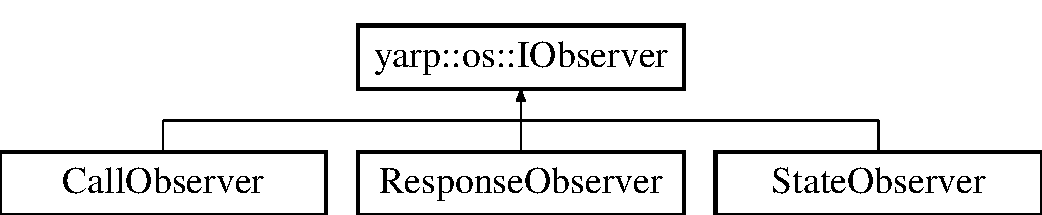
\includegraphics[height=2cm]{classyarp_1_1os_1_1_i_observer}
\end{center}
\end{figure}
\subsection*{Public Member Functions}
\begin{DoxyCompactItemize}
\item 
virtual \hyperlink{classyarp_1_1os_1_1_i_observer_a6e20a4a7baa318b53d6a7e3f198699f6}{$\sim$IObserver} ()
\item 
virtual void \hyperlink{classyarp_1_1os_1_1_i_observer_a4829e5a6f2ba6666b9539a4a30f20790}{onDataObserved} (yarp::os::Bottle \&b)=0
\item 
virtual \hyperlink{classyarp_1_1os_1_1_i_observer_a6e20a4a7baa318b53d6a7e3f198699f6}{$\sim$IObserver} ()
\item 
virtual void \hyperlink{classyarp_1_1os_1_1_i_observer_a4829e5a6f2ba6666b9539a4a30f20790}{onDataObserved} (yarp::os::Bottle \&b)=0
\end{DoxyCompactItemize}


\subsection{Detailed Description}
Interface that must be implemented to be able to be informed about information flowing in and out of filters (\hyperlink{classyarp_1_1os_1_1_rpc_filter}{RpcFilter} as well as \hyperlink{classyarp_1_1os_1_1_stream_filter}{StreamFilter}). 

\subsection{Constructor \& Destructor Documentation}
\hypertarget{classyarp_1_1os_1_1_i_observer_a6e20a4a7baa318b53d6a7e3f198699f6}{
\index{yarp::os::IObserver@{yarp::os::IObserver}!$\sim$IObserver@{$\sim$IObserver}}
\index{$\sim$IObserver@{$\sim$IObserver}!yarp::os::IObserver@{yarp::os::IObserver}}
\subsubsection[{$\sim$IObserver}]{\setlength{\rightskip}{0pt plus 5cm}virtual yarp::os::IObserver::$\sim$IObserver ()\hspace{0.3cm}{\ttfamily  \mbox{[}inline, virtual\mbox{]}}}}
\label{classyarp_1_1os_1_1_i_observer_a6e20a4a7baa318b53d6a7e3f198699f6}
\hypertarget{classyarp_1_1os_1_1_i_observer_a6e20a4a7baa318b53d6a7e3f198699f6}{
\index{yarp::os::IObserver@{yarp::os::IObserver}!$\sim$IObserver@{$\sim$IObserver}}
\index{$\sim$IObserver@{$\sim$IObserver}!yarp::os::IObserver@{yarp::os::IObserver}}
\subsubsection[{$\sim$IObserver}]{\setlength{\rightskip}{0pt plus 5cm}virtual yarp::os::IObserver::$\sim$IObserver ()\hspace{0.3cm}{\ttfamily  \mbox{[}inline, virtual\mbox{]}}}}
\label{classyarp_1_1os_1_1_i_observer_a6e20a4a7baa318b53d6a7e3f198699f6}


\subsection{Member Function Documentation}
\hypertarget{classyarp_1_1os_1_1_i_observer_a4829e5a6f2ba6666b9539a4a30f20790}{
\index{yarp::os::IObserver@{yarp::os::IObserver}!onDataObserved@{onDataObserved}}
\index{onDataObserved@{onDataObserved}!yarp::os::IObserver@{yarp::os::IObserver}}
\subsubsection[{onDataObserved}]{\setlength{\rightskip}{0pt plus 5cm}virtual void yarp::os::IObserver::onDataObserved (yarp::os::Bottle \& {\em b})\hspace{0.3cm}{\ttfamily  \mbox{[}pure virtual\mbox{]}}}}
\label{classyarp_1_1os_1_1_i_observer_a4829e5a6f2ba6666b9539a4a30f20790}
This function is called by filters to inform the implementing objects on data flowing in or out a the calling filter (\hyperlink{classyarp_1_1os_1_1_rpc_filter}{RpcFilter} as well as \hyperlink{classyarp_1_1os_1_1_stream_filter}{StreamFilter}). 

Implemented in \hyperlink{class_call_observer_abc1974fe2f04101dbbb1ae3ce83e7bfe}{CallObserver}, \hyperlink{class_response_observer_a2d847c448b31b5aa880b9282f7bf223d}{ResponseObserver}, and \hyperlink{class_state_observer_af104fa553abf31754d9acc084e9aa31f}{StateObserver}.\hypertarget{classyarp_1_1os_1_1_i_observer_a4829e5a6f2ba6666b9539a4a30f20790}{
\index{yarp::os::IObserver@{yarp::os::IObserver}!onDataObserved@{onDataObserved}}
\index{onDataObserved@{onDataObserved}!yarp::os::IObserver@{yarp::os::IObserver}}
\subsubsection[{onDataObserved}]{\setlength{\rightskip}{0pt plus 5cm}virtual void yarp::os::IObserver::onDataObserved (yarp::os::Bottle \& {\em b})\hspace{0.3cm}{\ttfamily  \mbox{[}pure virtual\mbox{]}}}}
\label{classyarp_1_1os_1_1_i_observer_a4829e5a6f2ba6666b9539a4a30f20790}
This function is called by filters to inform the implementing objects on data flowing in or out a the calling filter (\hyperlink{classyarp_1_1os_1_1_rpc_filter}{RpcFilter} as well as \hyperlink{classyarp_1_1os_1_1_stream_filter}{StreamFilter}). 

Implemented in \hyperlink{class_call_observer_abc1974fe2f04101dbbb1ae3ce83e7bfe}{CallObserver}, \hyperlink{class_response_observer_a2d847c448b31b5aa880b9282f7bf223d}{ResponseObserver}, and \hyperlink{class_state_observer_af104fa553abf31754d9acc084e9aa31f}{StateObserver}.

The documentation for this class was generated from the following files:\begin{DoxyCompactItemize}
\item 
/Users/kail/imClever/dev/virtualSkin/include/yarp/os/\hyperlink{include_2yarp_2os_2_i_observer_8h}{IObserver.h}\item 
/Users/kail/imClever/dev/virtualSkin/src/yarpUtil/gregorFilter/yarp/os/\hyperlink{src_2yarp_util_2gregor_filter_2yarp_2os_2_i_observer_8h}{IObserver.h}\end{DoxyCompactItemize}

\hypertarget{classyarp_1_1os_1_1_i_replier}{
\section{yarp::os::IReplier Class Reference}
\label{classyarp_1_1os_1_1_i_replier}\index{yarp::os::IReplier@{yarp::os::IReplier}}
}


{\ttfamily \#include $<$IReplier.h$>$}\subsection*{Public Member Functions}
\begin{DoxyCompactItemize}
\item 
virtual \hyperlink{classyarp_1_1os_1_1_i_replier_a197fe86812f17bc97cc7bf1b94473e84}{$\sim$IReplier} ()
\item 
virtual Bottle $\ast$ \hyperlink{classyarp_1_1os_1_1_i_replier_a6b14c9b19625876caa5843b15537dcbd}{getNextReponse} ()=0
\item 
virtual \hyperlink{classyarp_1_1os_1_1_i_replier_a197fe86812f17bc97cc7bf1b94473e84}{$\sim$IReplier} ()
\item 
virtual Bottle $\ast$ \hyperlink{classyarp_1_1os_1_1_i_replier_a6b14c9b19625876caa5843b15537dcbd}{getNextReponse} ()=0
\end{DoxyCompactItemize}


\subsection{Detailed Description}
Interface that must be implemented to be able to inject responses into \hyperlink{classyarp_1_1os_1_1_rpc_filter}{RpcFilter} s.

\begin{Desc}
\item[\hyperlink{todo__todo000007}{Todo}]Use auto\_\-ptr to return the bottle (I always get the error ISO C++ forbids declaration of 'auto\_\-ptr' with no type) \end{Desc}


Interface that must be implemented to be able to inject responses into \hyperlink{classyarp_1_1os_1_1_rpc_filter}{RpcFilter} s.

\begin{Desc}
\item[\hyperlink{todo__todo000017}{Todo}]Use auto\_\-ptr to return the bottle (I always get the error ISO C++ forbids declaration of 'auto\_\-ptr' with no type) \end{Desc}


\subsection{Constructor \& Destructor Documentation}
\hypertarget{classyarp_1_1os_1_1_i_replier_a197fe86812f17bc97cc7bf1b94473e84}{
\index{yarp::os::IReplier@{yarp::os::IReplier}!$\sim$IReplier@{$\sim$IReplier}}
\index{$\sim$IReplier@{$\sim$IReplier}!yarp::os::IReplier@{yarp::os::IReplier}}
\subsubsection[{$\sim$IReplier}]{\setlength{\rightskip}{0pt plus 5cm}virtual yarp::os::IReplier::$\sim$IReplier ()\hspace{0.3cm}{\ttfamily  \mbox{[}inline, virtual\mbox{]}}}}
\label{classyarp_1_1os_1_1_i_replier_a197fe86812f17bc97cc7bf1b94473e84}
\hypertarget{classyarp_1_1os_1_1_i_replier_a197fe86812f17bc97cc7bf1b94473e84}{
\index{yarp::os::IReplier@{yarp::os::IReplier}!$\sim$IReplier@{$\sim$IReplier}}
\index{$\sim$IReplier@{$\sim$IReplier}!yarp::os::IReplier@{yarp::os::IReplier}}
\subsubsection[{$\sim$IReplier}]{\setlength{\rightskip}{0pt plus 5cm}virtual yarp::os::IReplier::$\sim$IReplier ()\hspace{0.3cm}{\ttfamily  \mbox{[}inline, virtual\mbox{]}}}}
\label{classyarp_1_1os_1_1_i_replier_a197fe86812f17bc97cc7bf1b94473e84}


\subsection{Member Function Documentation}
\hypertarget{classyarp_1_1os_1_1_i_replier_a6b14c9b19625876caa5843b15537dcbd}{
\index{yarp::os::IReplier@{yarp::os::IReplier}!getNextReponse@{getNextReponse}}
\index{getNextReponse@{getNextReponse}!yarp::os::IReplier@{yarp::os::IReplier}}
\subsubsection[{getNextReponse}]{\setlength{\rightskip}{0pt plus 5cm}virtual Bottle$\ast$ yarp::os::IReplier::getNextReponse ()\hspace{0.3cm}{\ttfamily  \mbox{[}pure virtual\mbox{]}}}}
\label{classyarp_1_1os_1_1_i_replier_a6b14c9b19625876caa5843b15537dcbd}
\hypertarget{classyarp_1_1os_1_1_i_replier_a6b14c9b19625876caa5843b15537dcbd}{
\index{yarp::os::IReplier@{yarp::os::IReplier}!getNextReponse@{getNextReponse}}
\index{getNextReponse@{getNextReponse}!yarp::os::IReplier@{yarp::os::IReplier}}
\subsubsection[{getNextReponse}]{\setlength{\rightskip}{0pt plus 5cm}virtual Bottle$\ast$ yarp::os::IReplier::getNextReponse ()\hspace{0.3cm}{\ttfamily  \mbox{[}pure virtual\mbox{]}}}}
\label{classyarp_1_1os_1_1_i_replier_a6b14c9b19625876caa5843b15537dcbd}


The documentation for this class was generated from the following files:\begin{DoxyCompactItemize}
\item 
/Users/kail/imClever/dev/virtualSkin/include/yarp/os/\hyperlink{include_2yarp_2os_2_i_replier_8h}{IReplier.h}\item 
/Users/kail/imClever/dev/virtualSkin/src/yarpUtil/gregorFilter/yarp/os/\hyperlink{src_2yarp_util_2gregor_filter_2yarp_2os_2_i_replier_8h}{IReplier.h}\end{DoxyCompactItemize}

\hypertarget{class_robot_model_1_1_joint}{
\section{RobotModel::Joint Class Reference}
\label{class_robot_model_1_1_joint}\index{RobotModel::Joint@{RobotModel::Joint}}
}


{\ttfamily \#include $<$joint.h$>$}Inheritance diagram for RobotModel::Joint::\begin{figure}[H]
\begin{center}
\leavevmode
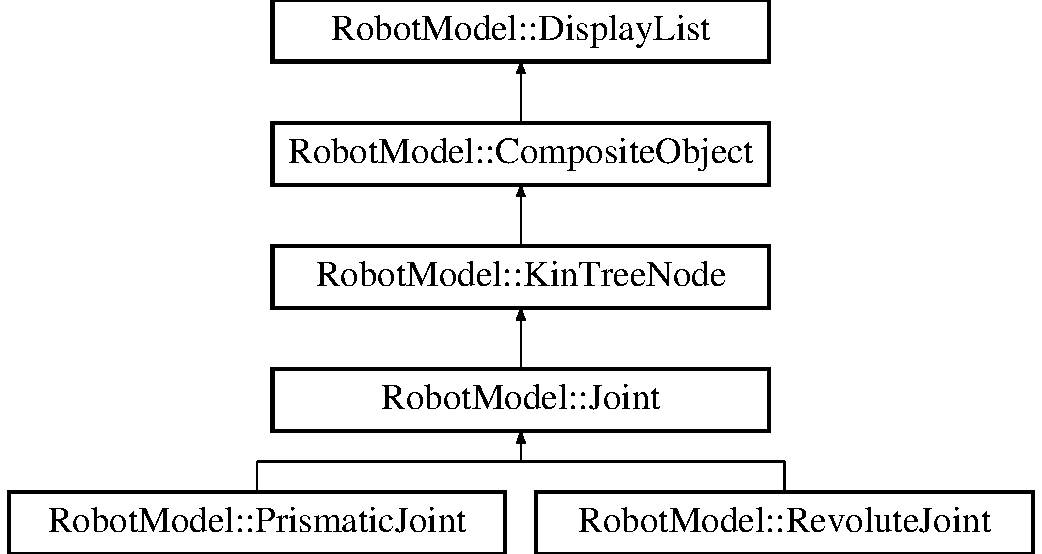
\includegraphics[height=2.23404cm]{class_robot_model_1_1_joint}
\end{center}
\end{figure}
\subsection*{Public Member Functions}
\begin{DoxyCompactItemize}
\item 
\hyperlink{class_robot_model_1_1_joint_ac0077acd1f45742c84c3468cce889600}{Joint} (\hyperlink{class_robot_model_1_1_robot}{Robot} $\ast$robot, \hyperlink{class_robot_model_1_1_kin_tree_node}{KinTreeNode} $\ast$parent, \hyperlink{class_robot_model_1_1_motor}{Motor} $\ast$\hyperlink{class_robot_model_1_1_joint_a8e8165df2271b16ab446028ee6bfa1c6}{motor}, \hyperlink{class_robot_model_1_1_kin_tree_node_a6cc10fb82046bd1d9f61b806756ad176}{Type} type)
\item 
virtual \hyperlink{class_robot_model_1_1_joint_a42aca0bd1832136984923713127c28f1}{$\sim$Joint} ()
\item 
void \hyperlink{class_robot_model_1_1_joint_ad982580bf8c0d721babaf93d990cf5d7}{setMin} (qreal pos)
\item 
void \hyperlink{class_robot_model_1_1_joint_a48523fd1cf98af4b0856257cde75f486}{setMax} (qreal pos)
\item 
void \hyperlink{class_robot_model_1_1_joint_a4fc5a8c53c2a2c5839409d90fb0825e1}{setPos} ()
\item 
\hyperlink{class_robot_model_1_1_joint_ace81033ec821f5bcb7e15c5ac1a84946}{Joint} (\hyperlink{class_robot_model_1_1_robot}{Robot} $\ast$robot, \hyperlink{class_robot_model_1_1_kin_tree_node}{KinTreeNode} $\ast$parent, \hyperlink{class_robot_model_1_1_motor}{Motor} $\ast$\hyperlink{class_robot_model_1_1_joint_a8e8165df2271b16ab446028ee6bfa1c6}{motor}, \hyperlink{class_robot_model_1_1_kin_tree_node_a6cc10fb82046bd1d9f61b806756ad176}{Type} type)
\item 
virtual \hyperlink{class_robot_model_1_1_joint_a191470d2376b08f2f3debc15d5e89ad0}{$\sim$Joint} ()
\item 
void \hyperlink{class_robot_model_1_1_joint_ad982580bf8c0d721babaf93d990cf5d7}{setMin} (qreal pos)
\item 
void \hyperlink{class_robot_model_1_1_joint_a48523fd1cf98af4b0856257cde75f486}{setMax} (qreal pos)
\item 
void \hyperlink{class_robot_model_1_1_joint_a816fef4ec39f5a4239540ba5a7011d6a}{setPos} ()
\end{DoxyCompactItemize}
\subsection*{Protected Member Functions}
\begin{DoxyCompactItemize}
\item 
virtual void \hyperlink{class_robot_model_1_1_joint_a485f5fc46f5156a7383bee7edbfc6643}{setM} ()=0
\item 
virtual void \hyperlink{class_robot_model_1_1_joint_a485f5fc46f5156a7383bee7edbfc6643}{setM} ()=0
\end{DoxyCompactItemize}
\subsection*{Protected Attributes}
\begin{DoxyCompactItemize}
\item 
\hyperlink{class_robot_model_1_1_motor}{Motor} $\ast$ \hyperlink{class_robot_model_1_1_joint_a8e8165df2271b16ab446028ee6bfa1c6}{motor}
\item 
qreal \hyperlink{class_robot_model_1_1_joint_aada2db465b0f51975a3c928656a9924c}{position}
\item 
\hyperlink{class_robot_model_1_1_interval}{Interval} \hyperlink{class_robot_model_1_1_joint_a3991756cd74729b87bde02b679c95b4c}{limits}
\end{DoxyCompactItemize}


\subsection{Constructor \& Destructor Documentation}
\hypertarget{class_robot_model_1_1_joint_ac0077acd1f45742c84c3468cce889600}{
\index{RobotModel::Joint@{RobotModel::Joint}!Joint@{Joint}}
\index{Joint@{Joint}!RobotModel::Joint@{RobotModel::Joint}}
\subsubsection[{Joint}]{\setlength{\rightskip}{0pt plus 5cm}Joint::Joint ({\bf Robot} $\ast$ {\em robot}, \/  {\bf KinTreeNode} $\ast$ {\em parent}, \/  {\bf Motor} $\ast$ {\em motor}, \/  {\bf KinTreeNode::Type} {\em type})}}
\label{class_robot_model_1_1_joint_ac0077acd1f45742c84c3468cce889600}
\hypertarget{class_robot_model_1_1_joint_a42aca0bd1832136984923713127c28f1}{
\index{RobotModel::Joint@{RobotModel::Joint}!$\sim$Joint@{$\sim$Joint}}
\index{$\sim$Joint@{$\sim$Joint}!RobotModel::Joint@{RobotModel::Joint}}
\subsubsection[{$\sim$Joint}]{\setlength{\rightskip}{0pt plus 5cm}Joint::$\sim$Joint ()\hspace{0.3cm}{\ttfamily  \mbox{[}virtual\mbox{]}}}}
\label{class_robot_model_1_1_joint_a42aca0bd1832136984923713127c28f1}
\hypertarget{class_robot_model_1_1_joint_ace81033ec821f5bcb7e15c5ac1a84946}{
\index{RobotModel::Joint@{RobotModel::Joint}!Joint@{Joint}}
\index{Joint@{Joint}!RobotModel::Joint@{RobotModel::Joint}}
\subsubsection[{Joint}]{\setlength{\rightskip}{0pt plus 5cm}RobotModel::Joint::Joint ({\bf Robot} $\ast$ {\em robot}, \/  {\bf KinTreeNode} $\ast$ {\em parent}, \/  {\bf Motor} $\ast$ {\em motor}, \/  {\bf Type} {\em type})}}
\label{class_robot_model_1_1_joint_ace81033ec821f5bcb7e15c5ac1a84946}
\hypertarget{class_robot_model_1_1_joint_a191470d2376b08f2f3debc15d5e89ad0}{
\index{RobotModel::Joint@{RobotModel::Joint}!$\sim$Joint@{$\sim$Joint}}
\index{$\sim$Joint@{$\sim$Joint}!RobotModel::Joint@{RobotModel::Joint}}
\subsubsection[{$\sim$Joint}]{\setlength{\rightskip}{0pt plus 5cm}virtual RobotModel::Joint::$\sim$Joint ()\hspace{0.3cm}{\ttfamily  \mbox{[}virtual\mbox{]}}}}
\label{class_robot_model_1_1_joint_a191470d2376b08f2f3debc15d5e89ad0}


\subsection{Member Function Documentation}
\hypertarget{class_robot_model_1_1_joint_a485f5fc46f5156a7383bee7edbfc6643}{
\index{RobotModel::Joint@{RobotModel::Joint}!setM@{setM}}
\index{setM@{setM}!RobotModel::Joint@{RobotModel::Joint}}
\subsubsection[{setM}]{\setlength{\rightskip}{0pt plus 5cm}virtual void RobotModel::Joint::setM ()\hspace{0.3cm}{\ttfamily  \mbox{[}protected, pure virtual\mbox{]}}}}
\label{class_robot_model_1_1_joint_a485f5fc46f5156a7383bee7edbfc6643}


Implements \hyperlink{class_robot_model_1_1_kin_tree_node_a47574c65af53990455540547d8d00e9f}{RobotModel::KinTreeNode}.\hypertarget{class_robot_model_1_1_joint_a485f5fc46f5156a7383bee7edbfc6643}{
\index{RobotModel::Joint@{RobotModel::Joint}!setM@{setM}}
\index{setM@{setM}!RobotModel::Joint@{RobotModel::Joint}}
\subsubsection[{setM}]{\setlength{\rightskip}{0pt plus 5cm}virtual void RobotModel::Joint::setM ()\hspace{0.3cm}{\ttfamily  \mbox{[}protected, pure virtual\mbox{]}}}}
\label{class_robot_model_1_1_joint_a485f5fc46f5156a7383bee7edbfc6643}


Implements \hyperlink{class_robot_model_1_1_kin_tree_node_a47574c65af53990455540547d8d00e9f}{RobotModel::KinTreeNode}.\hypertarget{class_robot_model_1_1_joint_a48523fd1cf98af4b0856257cde75f486}{
\index{RobotModel::Joint@{RobotModel::Joint}!setMax@{setMax}}
\index{setMax@{setMax}!RobotModel::Joint@{RobotModel::Joint}}
\subsubsection[{setMax}]{\setlength{\rightskip}{0pt plus 5cm}void RobotModel::Joint::setMax (qreal {\em pos})\hspace{0.3cm}{\ttfamily  \mbox{[}inline\mbox{]}}}}
\label{class_robot_model_1_1_joint_a48523fd1cf98af4b0856257cde75f486}
\hypertarget{class_robot_model_1_1_joint_a48523fd1cf98af4b0856257cde75f486}{
\index{RobotModel::Joint@{RobotModel::Joint}!setMax@{setMax}}
\index{setMax@{setMax}!RobotModel::Joint@{RobotModel::Joint}}
\subsubsection[{setMax}]{\setlength{\rightskip}{0pt plus 5cm}void RobotModel::Joint::setMax (qreal {\em pos})\hspace{0.3cm}{\ttfamily  \mbox{[}inline\mbox{]}}}}
\label{class_robot_model_1_1_joint_a48523fd1cf98af4b0856257cde75f486}
\hypertarget{class_robot_model_1_1_joint_ad982580bf8c0d721babaf93d990cf5d7}{
\index{RobotModel::Joint@{RobotModel::Joint}!setMin@{setMin}}
\index{setMin@{setMin}!RobotModel::Joint@{RobotModel::Joint}}
\subsubsection[{setMin}]{\setlength{\rightskip}{0pt plus 5cm}void RobotModel::Joint::setMin (qreal {\em pos})\hspace{0.3cm}{\ttfamily  \mbox{[}inline\mbox{]}}}}
\label{class_robot_model_1_1_joint_ad982580bf8c0d721babaf93d990cf5d7}
\hypertarget{class_robot_model_1_1_joint_ad982580bf8c0d721babaf93d990cf5d7}{
\index{RobotModel::Joint@{RobotModel::Joint}!setMin@{setMin}}
\index{setMin@{setMin}!RobotModel::Joint@{RobotModel::Joint}}
\subsubsection[{setMin}]{\setlength{\rightskip}{0pt plus 5cm}void RobotModel::Joint::setMin (qreal {\em pos})\hspace{0.3cm}{\ttfamily  \mbox{[}inline\mbox{]}}}}
\label{class_robot_model_1_1_joint_ad982580bf8c0d721babaf93d990cf5d7}
\hypertarget{class_robot_model_1_1_joint_a816fef4ec39f5a4239540ba5a7011d6a}{
\index{RobotModel::Joint@{RobotModel::Joint}!setPos@{setPos}}
\index{setPos@{setPos}!RobotModel::Joint@{RobotModel::Joint}}
\subsubsection[{setPos}]{\setlength{\rightskip}{0pt plus 5cm}void RobotModel::Joint::setPos ()}}
\label{class_robot_model_1_1_joint_a816fef4ec39f5a4239540ba5a7011d6a}
\hypertarget{class_robot_model_1_1_joint_a4fc5a8c53c2a2c5839409d90fb0825e1}{
\index{RobotModel::Joint@{RobotModel::Joint}!setPos@{setPos}}
\index{setPos@{setPos}!RobotModel::Joint@{RobotModel::Joint}}
\subsubsection[{setPos}]{\setlength{\rightskip}{0pt plus 5cm}void Joint::setPos ()}}
\label{class_robot_model_1_1_joint_a4fc5a8c53c2a2c5839409d90fb0825e1}


\subsection{Member Data Documentation}
\hypertarget{class_robot_model_1_1_joint_a3991756cd74729b87bde02b679c95b4c}{
\index{RobotModel::Joint@{RobotModel::Joint}!limits@{limits}}
\index{limits@{limits}!RobotModel::Joint@{RobotModel::Joint}}
\subsubsection[{limits}]{\setlength{\rightskip}{0pt plus 5cm}{\bf Interval} {\bf RobotModel::Joint::limits}\hspace{0.3cm}{\ttfamily  \mbox{[}protected\mbox{]}}}}
\label{class_robot_model_1_1_joint_a3991756cd74729b87bde02b679c95b4c}
\hypertarget{class_robot_model_1_1_joint_a8e8165df2271b16ab446028ee6bfa1c6}{
\index{RobotModel::Joint@{RobotModel::Joint}!motor@{motor}}
\index{motor@{motor}!RobotModel::Joint@{RobotModel::Joint}}
\subsubsection[{motor}]{\setlength{\rightskip}{0pt plus 5cm}{\bf Motor} $\ast$ {\bf RobotModel::Joint::motor}\hspace{0.3cm}{\ttfamily  \mbox{[}protected\mbox{]}}}}
\label{class_robot_model_1_1_joint_a8e8165df2271b16ab446028ee6bfa1c6}
\hypertarget{class_robot_model_1_1_joint_aada2db465b0f51975a3c928656a9924c}{
\index{RobotModel::Joint@{RobotModel::Joint}!position@{position}}
\index{position@{position}!RobotModel::Joint@{RobotModel::Joint}}
\subsubsection[{position}]{\setlength{\rightskip}{0pt plus 5cm}qreal {\bf RobotModel::Joint::position}\hspace{0.3cm}{\ttfamily  \mbox{[}protected\mbox{]}}}}
\label{class_robot_model_1_1_joint_aada2db465b0f51975a3c928656a9924c}


The documentation for this class was generated from the following files:\begin{DoxyCompactItemize}
\item 
/Users/kail/imClever/dev/virtualSkin/include/robotModel/\hyperlink{include_2robot_model_2joint_8h}{joint.h}\item 
/Users/kail/imClever/dev/virtualSkin/src/robotModel/\hyperlink{src_2robot_model_2joint_8h}{joint.h}\item 
/Users/kail/imClever/dev/virtualSkin/src/robotModel/\hyperlink{joint_8cpp}{joint.cpp}\end{DoxyCompactItemize}

\hypertarget{class_robot_model_1_1_kin_tree_node}{
\section{RobotModel::KinTreeNode Class Reference}
\label{class_robot_model_1_1_kin_tree_node}\index{RobotModel::KinTreeNode@{RobotModel::KinTreeNode}}
}


{\ttfamily \#include $<$kintreenode.h$>$}Inheritance diagram for RobotModel::KinTreeNode::\begin{figure}[H]
\begin{center}
\leavevmode
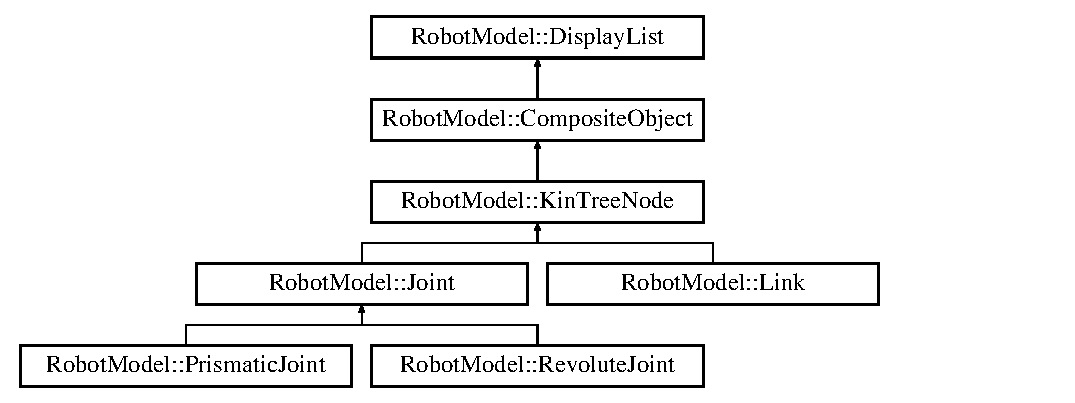
\includegraphics[height=4.76596cm]{class_robot_model_1_1_kin_tree_node}
\end{center}
\end{figure}
\subsection*{Public Types}
\begin{DoxyCompactItemize}
\item 
enum \hyperlink{class_robot_model_1_1_kin_tree_node_a6cc10fb82046bd1d9f61b806756ad176}{Type} \{ \par
\hyperlink{class_robot_model_1_1_kin_tree_node_a6cc10fb82046bd1d9f61b806756ad176abdf4c8f9138f4bfeb895532fbcbdcc83}{LINK}, 
\hyperlink{class_robot_model_1_1_kin_tree_node_a6cc10fb82046bd1d9f61b806756ad176a0f1b46f1ecc3b25851daa282aba9f441}{RJOINT}, 
\hyperlink{class_robot_model_1_1_kin_tree_node_a6cc10fb82046bd1d9f61b806756ad176ae49f45df694b20639cda99b5bc3dc15e}{PJOINT}, 
\hyperlink{class_robot_model_1_1_kin_tree_node_a6cc10fb82046bd1d9f61b806756ad176abdf4c8f9138f4bfeb895532fbcbdcc83}{LINK}, 
\par
\hyperlink{class_robot_model_1_1_kin_tree_node_a6cc10fb82046bd1d9f61b806756ad176a0f1b46f1ecc3b25851daa282aba9f441}{RJOINT}, 
\hyperlink{class_robot_model_1_1_kin_tree_node_a6cc10fb82046bd1d9f61b806756ad176ae49f45df694b20639cda99b5bc3dc15e}{PJOINT}
 \}
\item 
enum \hyperlink{class_robot_model_1_1_kin_tree_node_a6cc10fb82046bd1d9f61b806756ad176}{Type} \{ \par
\hyperlink{class_robot_model_1_1_kin_tree_node_a6cc10fb82046bd1d9f61b806756ad176abdf4c8f9138f4bfeb895532fbcbdcc83}{LINK}, 
\hyperlink{class_robot_model_1_1_kin_tree_node_a6cc10fb82046bd1d9f61b806756ad176a0f1b46f1ecc3b25851daa282aba9f441}{RJOINT}, 
\hyperlink{class_robot_model_1_1_kin_tree_node_a6cc10fb82046bd1d9f61b806756ad176ae49f45df694b20639cda99b5bc3dc15e}{PJOINT}, 
\hyperlink{class_robot_model_1_1_kin_tree_node_a6cc10fb82046bd1d9f61b806756ad176abdf4c8f9138f4bfeb895532fbcbdcc83}{LINK}, 
\par
\hyperlink{class_robot_model_1_1_kin_tree_node_a6cc10fb82046bd1d9f61b806756ad176a0f1b46f1ecc3b25851daa282aba9f441}{RJOINT}, 
\hyperlink{class_robot_model_1_1_kin_tree_node_a6cc10fb82046bd1d9f61b806756ad176ae49f45df694b20639cda99b5bc3dc15e}{PJOINT}
 \}
\end{DoxyCompactItemize}
\subsection*{Public Member Functions}
\begin{DoxyCompactItemize}
\item 
\hyperlink{class_robot_model_1_1_kin_tree_node_a48236a64352c2187db6193069d598c86}{KinTreeNode} (\hyperlink{class_robot_model_1_1_robot}{Robot} $\ast$\hyperlink{class_robot_model_1_1_kin_tree_node_aabd31bc0263bb2a830bde65af0eba1a6}{parentRobot}, \hyperlink{class_robot_model_1_1_kin_tree_node}{KinTreeNode} $\ast$\hyperlink{class_robot_model_1_1_kin_tree_node_af2a0ed90edef2013eeadcd5b5174c420}{parentNode}, \hyperlink{class_robot_model_1_1_kin_tree_node_a6cc10fb82046bd1d9f61b806756ad176}{Type} type=LINK)
\item 
virtual \hyperlink{class_robot_model_1_1_kin_tree_node_a629cf524084ee233b402674cb371195f}{$\sim$KinTreeNode} ()
\item 
void \hyperlink{class_robot_model_1_1_kin_tree_node_ae62ad98d6c2151232c20f1542c81a38b}{setNodeAxis} (const QVector3D \&vector)
\item 
\hyperlink{class_robot_model_1_1_kin_tree_node}{KinTreeNode} $\ast$ \hyperlink{class_robot_model_1_1_kin_tree_node_a58fa5e8933de90d3f4896d39292baa39}{parent} () const 
\item 
\hyperlink{class_robot_model_1_1_robot}{Robot} $\ast$ \hyperlink{class_robot_model_1_1_kin_tree_node_a7bd810e1df470e3d8801ac8f1aa0a60f}{robot} () const 
\item 
const int \hyperlink{class_robot_model_1_1_kin_tree_node_aec76eade3020c48bd3767e5acd330a49}{idx} () const 
\item 
const \hyperlink{class_robot_model_1_1_kin_tree_node_a6cc10fb82046bd1d9f61b806756ad176}{Type} \& \hyperlink{class_robot_model_1_1_kin_tree_node_aac3f58f3a0535b2983e2b328d9eee65a}{getNodeType} () const 
\item 
const QVector3D \& \hyperlink{class_robot_model_1_1_kin_tree_node_af6a4b3bd148bf6aba766c367e13d59b6}{getNodeAxis} () const 
\item 
const QMatrix4x4 \& \hyperlink{class_robot_model_1_1_kin_tree_node_a5c91c678cc74412ec298e61a39b47e3e}{getM} () const 
\item 
void \hyperlink{class_robot_model_1_1_kin_tree_node_af043fc57074a449364d2a6ec09be46a3}{append} (\hyperlink{class_robot_model_1_1_primitive_object}{PrimitiveObject} $\ast$primitive)
\item 
bool \hyperlink{class_robot_model_1_1_kin_tree_node_ac87cf9db956705dcee63f4dbc01cc664}{remove} (\hyperlink{class_robot_model_1_1_primitive_object}{PrimitiveObject} $\ast$primitive)
\item 
void \hyperlink{class_robot_model_1_1_kin_tree_node_a85f4364980f9144471b9d92e175c539e}{render} ()
\item 
void \hyperlink{class_robot_model_1_1_kin_tree_node_a51113339b5ffc471c058218f1294d73a}{filterCollisionPairs} ()
\item 
void \hyperlink{class_robot_model_1_1_kin_tree_node_adc5e295285315ab45b65c1dceeee1770}{serialFilter} (\hyperlink{class_robot_model_1_1_kin_tree_node}{KinTreeNode} $\ast$node, bool link=false, bool joint=false)
\item 
void \hyperlink{class_robot_model_1_1_kin_tree_node_a7edaa7f382637f6a15c3af68f4dfc7ab}{update} (const QMatrix4x4 \&txfr)
\item 
void \hyperlink{class_robot_model_1_1_kin_tree_node_ae5d72a496f39cad4e266c11d75d4731c}{notColliding} ()
\item 
void \hyperlink{class_robot_model_1_1_kin_tree_node_a788349199227101ec9e5a478842a1959}{print} () const 
\item 
void \hyperlink{class_robot_model_1_1_kin_tree_node_af682a96a09f754e0fb82066560538241}{printAll} ()
\item 
\hyperlink{class_robot_model_1_1_kin_tree_node_a0ee910d623799e97855e387b052cb83a}{KinTreeNode} (\hyperlink{class_robot_model_1_1_robot}{Robot} $\ast$\hyperlink{class_robot_model_1_1_kin_tree_node_aabd31bc0263bb2a830bde65af0eba1a6}{parentRobot}, \hyperlink{class_robot_model_1_1_kin_tree_node}{KinTreeNode} $\ast$\hyperlink{class_robot_model_1_1_kin_tree_node_af2a0ed90edef2013eeadcd5b5174c420}{parentNode}, \hyperlink{class_robot_model_1_1_kin_tree_node_a6cc10fb82046bd1d9f61b806756ad176}{Type} type=LINK)
\item 
virtual \hyperlink{class_robot_model_1_1_kin_tree_node_acff03d8aed8a974e50082449f289992c}{$\sim$KinTreeNode} ()
\item 
void \hyperlink{class_robot_model_1_1_kin_tree_node_a5621900c9c0d0fba3ce350dd446403e8}{setNodeAxis} (const QVector3D \&vector)
\item 
\hyperlink{class_robot_model_1_1_kin_tree_node}{KinTreeNode} $\ast$ \hyperlink{class_robot_model_1_1_kin_tree_node_a58fa5e8933de90d3f4896d39292baa39}{parent} () const 
\item 
\hyperlink{class_robot_model_1_1_robot}{Robot} $\ast$ \hyperlink{class_robot_model_1_1_kin_tree_node_a7bd810e1df470e3d8801ac8f1aa0a60f}{robot} () const 
\item 
const int \hyperlink{class_robot_model_1_1_kin_tree_node_aec76eade3020c48bd3767e5acd330a49}{idx} () const 
\item 
const \hyperlink{class_robot_model_1_1_kin_tree_node_a6cc10fb82046bd1d9f61b806756ad176}{Type} \& \hyperlink{class_robot_model_1_1_kin_tree_node_aac3f58f3a0535b2983e2b328d9eee65a}{getNodeType} () const 
\item 
const QVector3D \& \hyperlink{class_robot_model_1_1_kin_tree_node_af6a4b3bd148bf6aba766c367e13d59b6}{getNodeAxis} () const 
\item 
const QMatrix4x4 \& \hyperlink{class_robot_model_1_1_kin_tree_node_a5c91c678cc74412ec298e61a39b47e3e}{getM} () const 
\item 
void \hyperlink{class_robot_model_1_1_kin_tree_node_ae488de9b7fc97fb20690f66fead07391}{append} (\hyperlink{class_robot_model_1_1_primitive_object}{PrimitiveObject} $\ast$primitive)
\item 
bool \hyperlink{class_robot_model_1_1_kin_tree_node_a9612cdc54c0a34148ca5350b19a1d385}{remove} (\hyperlink{class_robot_model_1_1_primitive_object}{PrimitiveObject} $\ast$primitive)
\item 
void \hyperlink{class_robot_model_1_1_kin_tree_node_a7ccf98213f418d0e5efa4f699d898f2d}{render} ()
\item 
void \hyperlink{class_robot_model_1_1_kin_tree_node_a560df50c25717025df7a4682968b7319}{filterCollisionPairs} ()
\item 
void \hyperlink{class_robot_model_1_1_kin_tree_node_ac1aaeb1bf262448d159f9648a190c167}{serialFilter} (\hyperlink{class_robot_model_1_1_kin_tree_node}{KinTreeNode} $\ast$node, bool link=false, bool joint=false)
\item 
void \hyperlink{class_robot_model_1_1_kin_tree_node_a035b82b85c6a5f54e027bc05684f1032}{update} (const QMatrix4x4 \&txfr)
\item 
void \hyperlink{class_robot_model_1_1_kin_tree_node_a08e95447cbb2963b03afbac17215aa00}{notColliding} ()
\item 
void \hyperlink{class_robot_model_1_1_kin_tree_node_ae59d71f257f19e074d6f88cd2dd3c710}{print} () const 
\item 
void \hyperlink{class_robot_model_1_1_kin_tree_node_ab3136d2833d86ee76b22066de34a562c}{printAll} ()
\end{DoxyCompactItemize}
\subsection*{Protected Member Functions}
\begin{DoxyCompactItemize}
\item 
virtual void \hyperlink{class_robot_model_1_1_kin_tree_node_a47574c65af53990455540547d8d00e9f}{setM} ()=0
\item 
virtual void \hyperlink{class_robot_model_1_1_kin_tree_node_a47574c65af53990455540547d8d00e9f}{setM} ()=0
\end{DoxyCompactItemize}
\subsection*{Protected Attributes}
\begin{DoxyCompactItemize}
\item 
\hyperlink{class_robot_model_1_1_robot}{Robot} $\ast$ \hyperlink{class_robot_model_1_1_kin_tree_node_aabd31bc0263bb2a830bde65af0eba1a6}{parentRobot}
\item 
\hyperlink{class_robot_model_1_1_kin_tree_node}{KinTreeNode} $\ast$ \hyperlink{class_robot_model_1_1_kin_tree_node_af2a0ed90edef2013eeadcd5b5174c420}{parentNode}
\item 
int \hyperlink{class_robot_model_1_1_kin_tree_node_ab7be97fae982037992b0971ab25e643a}{index}
\item 
\hyperlink{class_robot_model_1_1_kin_tree_node_a6cc10fb82046bd1d9f61b806756ad176}{Type} \hyperlink{class_robot_model_1_1_kin_tree_node_acc89f79d42901042ca47a7b56761d4b1}{nodeType}
\item 
QVector$<$ \hyperlink{class_robot_model_1_1_kin_tree_node}{KinTreeNode} $\ast$ $>$ \hyperlink{class_robot_model_1_1_kin_tree_node_abf6a5c4792673635a7733ce24a749890}{children}
\item 
QVector3D \hyperlink{class_robot_model_1_1_kin_tree_node_af69707fb14705d4c1ab4ec6480e18b7e}{nodeAxis}
\item 
\hyperlink{class_robot_model_1_1_displ_matrix}{DisplMatrix} \hyperlink{class_robot_model_1_1_kin_tree_node_adc4909829a61513d89a23ebbf69d8243}{M}
\item 
QMutex \hyperlink{class_robot_model_1_1_kin_tree_node_ab2b663f51d01546b6e45be794a425438}{mutex}
\end{DoxyCompactItemize}


\subsection{Member Enumeration Documentation}
\hypertarget{class_robot_model_1_1_kin_tree_node_a6cc10fb82046bd1d9f61b806756ad176}{
\index{RobotModel::KinTreeNode@{RobotModel::KinTreeNode}!Type@{Type}}
\index{Type@{Type}!RobotModel::KinTreeNode@{RobotModel::KinTreeNode}}
\subsubsection[{Type}]{\setlength{\rightskip}{0pt plus 5cm}enum {\bf RobotModel::KinTreeNode::Type}}}
\label{class_robot_model_1_1_kin_tree_node_a6cc10fb82046bd1d9f61b806756ad176}
\begin{Desc}
\item[Enumerator: ]\par
\begin{description}
\index{LINK@{LINK}!RobotModel::KinTreeNode@{RobotModel::KinTreeNode}}\index{RobotModel::KinTreeNode@{RobotModel::KinTreeNode}!LINK@{LINK}}\item[{\em 
\hypertarget{class_robot_model_1_1_kin_tree_node_a6cc10fb82046bd1d9f61b806756ad176abdf4c8f9138f4bfeb895532fbcbdcc83}{
LINK}
\label{class_robot_model_1_1_kin_tree_node_a6cc10fb82046bd1d9f61b806756ad176abdf4c8f9138f4bfeb895532fbcbdcc83}
}]\index{RJOINT@{RJOINT}!RobotModel::KinTreeNode@{RobotModel::KinTreeNode}}\index{RobotModel::KinTreeNode@{RobotModel::KinTreeNode}!RJOINT@{RJOINT}}\item[{\em 
\hypertarget{class_robot_model_1_1_kin_tree_node_a6cc10fb82046bd1d9f61b806756ad176a0f1b46f1ecc3b25851daa282aba9f441}{
RJOINT}
\label{class_robot_model_1_1_kin_tree_node_a6cc10fb82046bd1d9f61b806756ad176a0f1b46f1ecc3b25851daa282aba9f441}
}]\index{PJOINT@{PJOINT}!RobotModel::KinTreeNode@{RobotModel::KinTreeNode}}\index{RobotModel::KinTreeNode@{RobotModel::KinTreeNode}!PJOINT@{PJOINT}}\item[{\em 
\hypertarget{class_robot_model_1_1_kin_tree_node_a6cc10fb82046bd1d9f61b806756ad176ae49f45df694b20639cda99b5bc3dc15e}{
PJOINT}
\label{class_robot_model_1_1_kin_tree_node_a6cc10fb82046bd1d9f61b806756ad176ae49f45df694b20639cda99b5bc3dc15e}
}]\index{LINK@{LINK}!RobotModel::KinTreeNode@{RobotModel::KinTreeNode}}\index{RobotModel::KinTreeNode@{RobotModel::KinTreeNode}!LINK@{LINK}}\item[{\em 
\hypertarget{class_robot_model_1_1_kin_tree_node_a6cc10fb82046bd1d9f61b806756ad176abdf4c8f9138f4bfeb895532fbcbdcc83}{
LINK}
\label{class_robot_model_1_1_kin_tree_node_a6cc10fb82046bd1d9f61b806756ad176abdf4c8f9138f4bfeb895532fbcbdcc83}
}]\index{RJOINT@{RJOINT}!RobotModel::KinTreeNode@{RobotModel::KinTreeNode}}\index{RobotModel::KinTreeNode@{RobotModel::KinTreeNode}!RJOINT@{RJOINT}}\item[{\em 
\hypertarget{class_robot_model_1_1_kin_tree_node_a6cc10fb82046bd1d9f61b806756ad176a0f1b46f1ecc3b25851daa282aba9f441}{
RJOINT}
\label{class_robot_model_1_1_kin_tree_node_a6cc10fb82046bd1d9f61b806756ad176a0f1b46f1ecc3b25851daa282aba9f441}
}]\index{PJOINT@{PJOINT}!RobotModel::KinTreeNode@{RobotModel::KinTreeNode}}\index{RobotModel::KinTreeNode@{RobotModel::KinTreeNode}!PJOINT@{PJOINT}}\item[{\em 
\hypertarget{class_robot_model_1_1_kin_tree_node_a6cc10fb82046bd1d9f61b806756ad176ae49f45df694b20639cda99b5bc3dc15e}{
PJOINT}
\label{class_robot_model_1_1_kin_tree_node_a6cc10fb82046bd1d9f61b806756ad176ae49f45df694b20639cda99b5bc3dc15e}
}]\end{description}
\end{Desc}

\hypertarget{class_robot_model_1_1_kin_tree_node_a6cc10fb82046bd1d9f61b806756ad176}{
\index{RobotModel::KinTreeNode@{RobotModel::KinTreeNode}!Type@{Type}}
\index{Type@{Type}!RobotModel::KinTreeNode@{RobotModel::KinTreeNode}}
\subsubsection[{Type}]{\setlength{\rightskip}{0pt plus 5cm}enum {\bf RobotModel::KinTreeNode::Type}}}
\label{class_robot_model_1_1_kin_tree_node_a6cc10fb82046bd1d9f61b806756ad176}
\begin{Desc}
\item[Enumerator: ]\par
\begin{description}
\index{LINK@{LINK}!RobotModel::KinTreeNode@{RobotModel::KinTreeNode}}\index{RobotModel::KinTreeNode@{RobotModel::KinTreeNode}!LINK@{LINK}}\item[{\em 
\hypertarget{class_robot_model_1_1_kin_tree_node_a6cc10fb82046bd1d9f61b806756ad176abdf4c8f9138f4bfeb895532fbcbdcc83}{
LINK}
\label{class_robot_model_1_1_kin_tree_node_a6cc10fb82046bd1d9f61b806756ad176abdf4c8f9138f4bfeb895532fbcbdcc83}
}]\index{RJOINT@{RJOINT}!RobotModel::KinTreeNode@{RobotModel::KinTreeNode}}\index{RobotModel::KinTreeNode@{RobotModel::KinTreeNode}!RJOINT@{RJOINT}}\item[{\em 
\hypertarget{class_robot_model_1_1_kin_tree_node_a6cc10fb82046bd1d9f61b806756ad176a0f1b46f1ecc3b25851daa282aba9f441}{
RJOINT}
\label{class_robot_model_1_1_kin_tree_node_a6cc10fb82046bd1d9f61b806756ad176a0f1b46f1ecc3b25851daa282aba9f441}
}]\index{PJOINT@{PJOINT}!RobotModel::KinTreeNode@{RobotModel::KinTreeNode}}\index{RobotModel::KinTreeNode@{RobotModel::KinTreeNode}!PJOINT@{PJOINT}}\item[{\em 
\hypertarget{class_robot_model_1_1_kin_tree_node_a6cc10fb82046bd1d9f61b806756ad176ae49f45df694b20639cda99b5bc3dc15e}{
PJOINT}
\label{class_robot_model_1_1_kin_tree_node_a6cc10fb82046bd1d9f61b806756ad176ae49f45df694b20639cda99b5bc3dc15e}
}]\index{LINK@{LINK}!RobotModel::KinTreeNode@{RobotModel::KinTreeNode}}\index{RobotModel::KinTreeNode@{RobotModel::KinTreeNode}!LINK@{LINK}}\item[{\em 
\hypertarget{class_robot_model_1_1_kin_tree_node_a6cc10fb82046bd1d9f61b806756ad176abdf4c8f9138f4bfeb895532fbcbdcc83}{
LINK}
\label{class_robot_model_1_1_kin_tree_node_a6cc10fb82046bd1d9f61b806756ad176abdf4c8f9138f4bfeb895532fbcbdcc83}
}]\index{RJOINT@{RJOINT}!RobotModel::KinTreeNode@{RobotModel::KinTreeNode}}\index{RobotModel::KinTreeNode@{RobotModel::KinTreeNode}!RJOINT@{RJOINT}}\item[{\em 
\hypertarget{class_robot_model_1_1_kin_tree_node_a6cc10fb82046bd1d9f61b806756ad176a0f1b46f1ecc3b25851daa282aba9f441}{
RJOINT}
\label{class_robot_model_1_1_kin_tree_node_a6cc10fb82046bd1d9f61b806756ad176a0f1b46f1ecc3b25851daa282aba9f441}
}]\index{PJOINT@{PJOINT}!RobotModel::KinTreeNode@{RobotModel::KinTreeNode}}\index{RobotModel::KinTreeNode@{RobotModel::KinTreeNode}!PJOINT@{PJOINT}}\item[{\em 
\hypertarget{class_robot_model_1_1_kin_tree_node_a6cc10fb82046bd1d9f61b806756ad176ae49f45df694b20639cda99b5bc3dc15e}{
PJOINT}
\label{class_robot_model_1_1_kin_tree_node_a6cc10fb82046bd1d9f61b806756ad176ae49f45df694b20639cda99b5bc3dc15e}
}]\end{description}
\end{Desc}



\subsection{Constructor \& Destructor Documentation}
\hypertarget{class_robot_model_1_1_kin_tree_node_a48236a64352c2187db6193069d598c86}{
\index{RobotModel::KinTreeNode@{RobotModel::KinTreeNode}!KinTreeNode@{KinTreeNode}}
\index{KinTreeNode@{KinTreeNode}!RobotModel::KinTreeNode@{RobotModel::KinTreeNode}}
\subsubsection[{KinTreeNode}]{\setlength{\rightskip}{0pt plus 5cm}KinTreeNode::KinTreeNode ({\bf Robot} $\ast$ {\em parentRobot}, \/  {\bf KinTreeNode} $\ast$ {\em parentNode}, \/  {\bf Type} {\em type} = {\ttfamily LINK})}}
\label{class_robot_model_1_1_kin_tree_node_a48236a64352c2187db6193069d598c86}
\hypertarget{class_robot_model_1_1_kin_tree_node_a629cf524084ee233b402674cb371195f}{
\index{RobotModel::KinTreeNode@{RobotModel::KinTreeNode}!$\sim$KinTreeNode@{$\sim$KinTreeNode}}
\index{$\sim$KinTreeNode@{$\sim$KinTreeNode}!RobotModel::KinTreeNode@{RobotModel::KinTreeNode}}
\subsubsection[{$\sim$KinTreeNode}]{\setlength{\rightskip}{0pt plus 5cm}KinTreeNode::$\sim$KinTreeNode ()\hspace{0.3cm}{\ttfamily  \mbox{[}virtual\mbox{]}}}}
\label{class_robot_model_1_1_kin_tree_node_a629cf524084ee233b402674cb371195f}
\hypertarget{class_robot_model_1_1_kin_tree_node_a0ee910d623799e97855e387b052cb83a}{
\index{RobotModel::KinTreeNode@{RobotModel::KinTreeNode}!KinTreeNode@{KinTreeNode}}
\index{KinTreeNode@{KinTreeNode}!RobotModel::KinTreeNode@{RobotModel::KinTreeNode}}
\subsubsection[{KinTreeNode}]{\setlength{\rightskip}{0pt plus 5cm}RobotModel::KinTreeNode::KinTreeNode ({\bf Robot} $\ast$ {\em parentRobot}, \/  {\bf KinTreeNode} $\ast$ {\em parentNode}, \/  {\bf Type} {\em type} = {\ttfamily LINK})}}
\label{class_robot_model_1_1_kin_tree_node_a0ee910d623799e97855e387b052cb83a}
\hypertarget{class_robot_model_1_1_kin_tree_node_acff03d8aed8a974e50082449f289992c}{
\index{RobotModel::KinTreeNode@{RobotModel::KinTreeNode}!$\sim$KinTreeNode@{$\sim$KinTreeNode}}
\index{$\sim$KinTreeNode@{$\sim$KinTreeNode}!RobotModel::KinTreeNode@{RobotModel::KinTreeNode}}
\subsubsection[{$\sim$KinTreeNode}]{\setlength{\rightskip}{0pt plus 5cm}virtual RobotModel::KinTreeNode::$\sim$KinTreeNode ()\hspace{0.3cm}{\ttfamily  \mbox{[}virtual\mbox{]}}}}
\label{class_robot_model_1_1_kin_tree_node_acff03d8aed8a974e50082449f289992c}


\subsection{Member Function Documentation}
\hypertarget{class_robot_model_1_1_kin_tree_node_ae488de9b7fc97fb20690f66fead07391}{
\index{RobotModel::KinTreeNode@{RobotModel::KinTreeNode}!append@{append}}
\index{append@{append}!RobotModel::KinTreeNode@{RobotModel::KinTreeNode}}
\subsubsection[{append}]{\setlength{\rightskip}{0pt plus 5cm}void RobotModel::KinTreeNode::append ({\bf PrimitiveObject} $\ast$ {\em primitive})\hspace{0.3cm}{\ttfamily  \mbox{[}virtual\mbox{]}}}}
\label{class_robot_model_1_1_kin_tree_node_ae488de9b7fc97fb20690f66fead07391}


Reimplemented from \hyperlink{class_robot_model_1_1_composite_object_ad33452f1246939d366ffbf02d1022a91}{RobotModel::CompositeObject}.\hypertarget{class_robot_model_1_1_kin_tree_node_af043fc57074a449364d2a6ec09be46a3}{
\index{RobotModel::KinTreeNode@{RobotModel::KinTreeNode}!append@{append}}
\index{append@{append}!RobotModel::KinTreeNode@{RobotModel::KinTreeNode}}
\subsubsection[{append}]{\setlength{\rightskip}{0pt plus 5cm}void KinTreeNode::append ({\bf PrimitiveObject} $\ast$ {\em primitive})\hspace{0.3cm}{\ttfamily  \mbox{[}virtual\mbox{]}}}}
\label{class_robot_model_1_1_kin_tree_node_af043fc57074a449364d2a6ec09be46a3}


Reimplemented from \hyperlink{class_robot_model_1_1_composite_object_ad33452f1246939d366ffbf02d1022a91}{RobotModel::CompositeObject}.\hypertarget{class_robot_model_1_1_kin_tree_node_a560df50c25717025df7a4682968b7319}{
\index{RobotModel::KinTreeNode@{RobotModel::KinTreeNode}!filterCollisionPairs@{filterCollisionPairs}}
\index{filterCollisionPairs@{filterCollisionPairs}!RobotModel::KinTreeNode@{RobotModel::KinTreeNode}}
\subsubsection[{filterCollisionPairs}]{\setlength{\rightskip}{0pt plus 5cm}void RobotModel::KinTreeNode::filterCollisionPairs ()}}
\label{class_robot_model_1_1_kin_tree_node_a560df50c25717025df7a4682968b7319}
\hypertarget{class_robot_model_1_1_kin_tree_node_a51113339b5ffc471c058218f1294d73a}{
\index{RobotModel::KinTreeNode@{RobotModel::KinTreeNode}!filterCollisionPairs@{filterCollisionPairs}}
\index{filterCollisionPairs@{filterCollisionPairs}!RobotModel::KinTreeNode@{RobotModel::KinTreeNode}}
\subsubsection[{filterCollisionPairs}]{\setlength{\rightskip}{0pt plus 5cm}void KinTreeNode::filterCollisionPairs ()}}
\label{class_robot_model_1_1_kin_tree_node_a51113339b5ffc471c058218f1294d73a}
\hypertarget{class_robot_model_1_1_kin_tree_node_a5c91c678cc74412ec298e61a39b47e3e}{
\index{RobotModel::KinTreeNode@{RobotModel::KinTreeNode}!getM@{getM}}
\index{getM@{getM}!RobotModel::KinTreeNode@{RobotModel::KinTreeNode}}
\subsubsection[{getM}]{\setlength{\rightskip}{0pt plus 5cm}const QMatrix4x4\& RobotModel::KinTreeNode::getM () const\hspace{0.3cm}{\ttfamily  \mbox{[}inline\mbox{]}}}}
\label{class_robot_model_1_1_kin_tree_node_a5c91c678cc74412ec298e61a39b47e3e}
\hypertarget{class_robot_model_1_1_kin_tree_node_a5c91c678cc74412ec298e61a39b47e3e}{
\index{RobotModel::KinTreeNode@{RobotModel::KinTreeNode}!getM@{getM}}
\index{getM@{getM}!RobotModel::KinTreeNode@{RobotModel::KinTreeNode}}
\subsubsection[{getM}]{\setlength{\rightskip}{0pt plus 5cm}const QMatrix4x4\& RobotModel::KinTreeNode::getM () const\hspace{0.3cm}{\ttfamily  \mbox{[}inline\mbox{]}}}}
\label{class_robot_model_1_1_kin_tree_node_a5c91c678cc74412ec298e61a39b47e3e}
\hypertarget{class_robot_model_1_1_kin_tree_node_af6a4b3bd148bf6aba766c367e13d59b6}{
\index{RobotModel::KinTreeNode@{RobotModel::KinTreeNode}!getNodeAxis@{getNodeAxis}}
\index{getNodeAxis@{getNodeAxis}!RobotModel::KinTreeNode@{RobotModel::KinTreeNode}}
\subsubsection[{getNodeAxis}]{\setlength{\rightskip}{0pt plus 5cm}const QVector3D\& RobotModel::KinTreeNode::getNodeAxis () const\hspace{0.3cm}{\ttfamily  \mbox{[}inline\mbox{]}}}}
\label{class_robot_model_1_1_kin_tree_node_af6a4b3bd148bf6aba766c367e13d59b6}
\hypertarget{class_robot_model_1_1_kin_tree_node_af6a4b3bd148bf6aba766c367e13d59b6}{
\index{RobotModel::KinTreeNode@{RobotModel::KinTreeNode}!getNodeAxis@{getNodeAxis}}
\index{getNodeAxis@{getNodeAxis}!RobotModel::KinTreeNode@{RobotModel::KinTreeNode}}
\subsubsection[{getNodeAxis}]{\setlength{\rightskip}{0pt plus 5cm}const QVector3D\& RobotModel::KinTreeNode::getNodeAxis () const\hspace{0.3cm}{\ttfamily  \mbox{[}inline\mbox{]}}}}
\label{class_robot_model_1_1_kin_tree_node_af6a4b3bd148bf6aba766c367e13d59b6}
\hypertarget{class_robot_model_1_1_kin_tree_node_aac3f58f3a0535b2983e2b328d9eee65a}{
\index{RobotModel::KinTreeNode@{RobotModel::KinTreeNode}!getNodeType@{getNodeType}}
\index{getNodeType@{getNodeType}!RobotModel::KinTreeNode@{RobotModel::KinTreeNode}}
\subsubsection[{getNodeType}]{\setlength{\rightskip}{0pt plus 5cm}const {\bf Type}\& RobotModel::KinTreeNode::getNodeType () const\hspace{0.3cm}{\ttfamily  \mbox{[}inline\mbox{]}}}}
\label{class_robot_model_1_1_kin_tree_node_aac3f58f3a0535b2983e2b328d9eee65a}
\hypertarget{class_robot_model_1_1_kin_tree_node_aac3f58f3a0535b2983e2b328d9eee65a}{
\index{RobotModel::KinTreeNode@{RobotModel::KinTreeNode}!getNodeType@{getNodeType}}
\index{getNodeType@{getNodeType}!RobotModel::KinTreeNode@{RobotModel::KinTreeNode}}
\subsubsection[{getNodeType}]{\setlength{\rightskip}{0pt plus 5cm}const {\bf Type}\& RobotModel::KinTreeNode::getNodeType () const\hspace{0.3cm}{\ttfamily  \mbox{[}inline\mbox{]}}}}
\label{class_robot_model_1_1_kin_tree_node_aac3f58f3a0535b2983e2b328d9eee65a}
\hypertarget{class_robot_model_1_1_kin_tree_node_aec76eade3020c48bd3767e5acd330a49}{
\index{RobotModel::KinTreeNode@{RobotModel::KinTreeNode}!idx@{idx}}
\index{idx@{idx}!RobotModel::KinTreeNode@{RobotModel::KinTreeNode}}
\subsubsection[{idx}]{\setlength{\rightskip}{0pt plus 5cm}const int RobotModel::KinTreeNode::idx () const\hspace{0.3cm}{\ttfamily  \mbox{[}inline\mbox{]}}}}
\label{class_robot_model_1_1_kin_tree_node_aec76eade3020c48bd3767e5acd330a49}
\hypertarget{class_robot_model_1_1_kin_tree_node_aec76eade3020c48bd3767e5acd330a49}{
\index{RobotModel::KinTreeNode@{RobotModel::KinTreeNode}!idx@{idx}}
\index{idx@{idx}!RobotModel::KinTreeNode@{RobotModel::KinTreeNode}}
\subsubsection[{idx}]{\setlength{\rightskip}{0pt plus 5cm}const int RobotModel::KinTreeNode::idx () const\hspace{0.3cm}{\ttfamily  \mbox{[}inline\mbox{]}}}}
\label{class_robot_model_1_1_kin_tree_node_aec76eade3020c48bd3767e5acd330a49}
\hypertarget{class_robot_model_1_1_kin_tree_node_a08e95447cbb2963b03afbac17215aa00}{
\index{RobotModel::KinTreeNode@{RobotModel::KinTreeNode}!notColliding@{notColliding}}
\index{notColliding@{notColliding}!RobotModel::KinTreeNode@{RobotModel::KinTreeNode}}
\subsubsection[{notColliding}]{\setlength{\rightskip}{0pt plus 5cm}void RobotModel::KinTreeNode::notColliding ()\hspace{0.3cm}{\ttfamily  \mbox{[}virtual\mbox{]}}}}
\label{class_robot_model_1_1_kin_tree_node_a08e95447cbb2963b03afbac17215aa00}


Reimplemented from \hyperlink{class_robot_model_1_1_composite_object_a00db0d1a45893ef058e7abbad5083b6b}{RobotModel::CompositeObject}.\hypertarget{class_robot_model_1_1_kin_tree_node_ae5d72a496f39cad4e266c11d75d4731c}{
\index{RobotModel::KinTreeNode@{RobotModel::KinTreeNode}!notColliding@{notColliding}}
\index{notColliding@{notColliding}!RobotModel::KinTreeNode@{RobotModel::KinTreeNode}}
\subsubsection[{notColliding}]{\setlength{\rightskip}{0pt plus 5cm}void KinTreeNode::notColliding ()\hspace{0.3cm}{\ttfamily  \mbox{[}virtual\mbox{]}}}}
\label{class_robot_model_1_1_kin_tree_node_ae5d72a496f39cad4e266c11d75d4731c}


Reimplemented from \hyperlink{class_robot_model_1_1_composite_object_a00db0d1a45893ef058e7abbad5083b6b}{RobotModel::CompositeObject}.\hypertarget{class_robot_model_1_1_kin_tree_node_a58fa5e8933de90d3f4896d39292baa39}{
\index{RobotModel::KinTreeNode@{RobotModel::KinTreeNode}!parent@{parent}}
\index{parent@{parent}!RobotModel::KinTreeNode@{RobotModel::KinTreeNode}}
\subsubsection[{parent}]{\setlength{\rightskip}{0pt plus 5cm}{\bf KinTreeNode}$\ast$ RobotModel::KinTreeNode::parent () const\hspace{0.3cm}{\ttfamily  \mbox{[}inline\mbox{]}}}}
\label{class_robot_model_1_1_kin_tree_node_a58fa5e8933de90d3f4896d39292baa39}
\hypertarget{class_robot_model_1_1_kin_tree_node_a58fa5e8933de90d3f4896d39292baa39}{
\index{RobotModel::KinTreeNode@{RobotModel::KinTreeNode}!parent@{parent}}
\index{parent@{parent}!RobotModel::KinTreeNode@{RobotModel::KinTreeNode}}
\subsubsection[{parent}]{\setlength{\rightskip}{0pt plus 5cm}{\bf KinTreeNode}$\ast$ RobotModel::KinTreeNode::parent () const\hspace{0.3cm}{\ttfamily  \mbox{[}inline\mbox{]}}}}
\label{class_robot_model_1_1_kin_tree_node_a58fa5e8933de90d3f4896d39292baa39}
\hypertarget{class_robot_model_1_1_kin_tree_node_ae59d71f257f19e074d6f88cd2dd3c710}{
\index{RobotModel::KinTreeNode@{RobotModel::KinTreeNode}!print@{print}}
\index{print@{print}!RobotModel::KinTreeNode@{RobotModel::KinTreeNode}}
\subsubsection[{print}]{\setlength{\rightskip}{0pt plus 5cm}void RobotModel::KinTreeNode::print () const}}
\label{class_robot_model_1_1_kin_tree_node_ae59d71f257f19e074d6f88cd2dd3c710}
\hypertarget{class_robot_model_1_1_kin_tree_node_a788349199227101ec9e5a478842a1959}{
\index{RobotModel::KinTreeNode@{RobotModel::KinTreeNode}!print@{print}}
\index{print@{print}!RobotModel::KinTreeNode@{RobotModel::KinTreeNode}}
\subsubsection[{print}]{\setlength{\rightskip}{0pt plus 5cm}void KinTreeNode::print () const}}
\label{class_robot_model_1_1_kin_tree_node_a788349199227101ec9e5a478842a1959}
\hypertarget{class_robot_model_1_1_kin_tree_node_ab3136d2833d86ee76b22066de34a562c}{
\index{RobotModel::KinTreeNode@{RobotModel::KinTreeNode}!printAll@{printAll}}
\index{printAll@{printAll}!RobotModel::KinTreeNode@{RobotModel::KinTreeNode}}
\subsubsection[{printAll}]{\setlength{\rightskip}{0pt plus 5cm}void RobotModel::KinTreeNode::printAll ()}}
\label{class_robot_model_1_1_kin_tree_node_ab3136d2833d86ee76b22066de34a562c}
\hypertarget{class_robot_model_1_1_kin_tree_node_af682a96a09f754e0fb82066560538241}{
\index{RobotModel::KinTreeNode@{RobotModel::KinTreeNode}!printAll@{printAll}}
\index{printAll@{printAll}!RobotModel::KinTreeNode@{RobotModel::KinTreeNode}}
\subsubsection[{printAll}]{\setlength{\rightskip}{0pt plus 5cm}void KinTreeNode::printAll ()}}
\label{class_robot_model_1_1_kin_tree_node_af682a96a09f754e0fb82066560538241}
\hypertarget{class_robot_model_1_1_kin_tree_node_a9612cdc54c0a34148ca5350b19a1d385}{
\index{RobotModel::KinTreeNode@{RobotModel::KinTreeNode}!remove@{remove}}
\index{remove@{remove}!RobotModel::KinTreeNode@{RobotModel::KinTreeNode}}
\subsubsection[{remove}]{\setlength{\rightskip}{0pt plus 5cm}bool RobotModel::KinTreeNode::remove ({\bf PrimitiveObject} $\ast$ {\em primitive})\hspace{0.3cm}{\ttfamily  \mbox{[}virtual\mbox{]}}}}
\label{class_robot_model_1_1_kin_tree_node_a9612cdc54c0a34148ca5350b19a1d385}


Reimplemented from \hyperlink{class_robot_model_1_1_composite_object_ac63de1955b6bda820d39c01616af8665}{RobotModel::CompositeObject}.\hypertarget{class_robot_model_1_1_kin_tree_node_ac87cf9db956705dcee63f4dbc01cc664}{
\index{RobotModel::KinTreeNode@{RobotModel::KinTreeNode}!remove@{remove}}
\index{remove@{remove}!RobotModel::KinTreeNode@{RobotModel::KinTreeNode}}
\subsubsection[{remove}]{\setlength{\rightskip}{0pt plus 5cm}bool KinTreeNode::remove ({\bf PrimitiveObject} $\ast$ {\em primitive})\hspace{0.3cm}{\ttfamily  \mbox{[}virtual\mbox{]}}}}
\label{class_robot_model_1_1_kin_tree_node_ac87cf9db956705dcee63f4dbc01cc664}


Reimplemented from \hyperlink{class_robot_model_1_1_composite_object_ac63de1955b6bda820d39c01616af8665}{RobotModel::CompositeObject}.\hypertarget{class_robot_model_1_1_kin_tree_node_a7ccf98213f418d0e5efa4f699d898f2d}{
\index{RobotModel::KinTreeNode@{RobotModel::KinTreeNode}!render@{render}}
\index{render@{render}!RobotModel::KinTreeNode@{RobotModel::KinTreeNode}}
\subsubsection[{render}]{\setlength{\rightskip}{0pt plus 5cm}void RobotModel::KinTreeNode::render ()\hspace{0.3cm}{\ttfamily  \mbox{[}virtual\mbox{]}}}}
\label{class_robot_model_1_1_kin_tree_node_a7ccf98213f418d0e5efa4f699d898f2d}


Reimplemented from \hyperlink{class_robot_model_1_1_composite_object_aee43da74b22f6272736844effe7a1dd6}{RobotModel::CompositeObject}.\hypertarget{class_robot_model_1_1_kin_tree_node_a85f4364980f9144471b9d92e175c539e}{
\index{RobotModel::KinTreeNode@{RobotModel::KinTreeNode}!render@{render}}
\index{render@{render}!RobotModel::KinTreeNode@{RobotModel::KinTreeNode}}
\subsubsection[{render}]{\setlength{\rightskip}{0pt plus 5cm}void KinTreeNode::render ()\hspace{0.3cm}{\ttfamily  \mbox{[}virtual\mbox{]}}}}
\label{class_robot_model_1_1_kin_tree_node_a85f4364980f9144471b9d92e175c539e}


Reimplemented from \hyperlink{class_robot_model_1_1_composite_object_aee43da74b22f6272736844effe7a1dd6}{RobotModel::CompositeObject}.\hypertarget{class_robot_model_1_1_kin_tree_node_a7bd810e1df470e3d8801ac8f1aa0a60f}{
\index{RobotModel::KinTreeNode@{RobotModel::KinTreeNode}!robot@{robot}}
\index{robot@{robot}!RobotModel::KinTreeNode@{RobotModel::KinTreeNode}}
\subsubsection[{robot}]{\setlength{\rightskip}{0pt plus 5cm}{\bf Robot}$\ast$ RobotModel::KinTreeNode::robot () const\hspace{0.3cm}{\ttfamily  \mbox{[}inline\mbox{]}}}}
\label{class_robot_model_1_1_kin_tree_node_a7bd810e1df470e3d8801ac8f1aa0a60f}
\hypertarget{class_robot_model_1_1_kin_tree_node_a7bd810e1df470e3d8801ac8f1aa0a60f}{
\index{RobotModel::KinTreeNode@{RobotModel::KinTreeNode}!robot@{robot}}
\index{robot@{robot}!RobotModel::KinTreeNode@{RobotModel::KinTreeNode}}
\subsubsection[{robot}]{\setlength{\rightskip}{0pt plus 5cm}{\bf Robot}$\ast$ RobotModel::KinTreeNode::robot () const\hspace{0.3cm}{\ttfamily  \mbox{[}inline\mbox{]}}}}
\label{class_robot_model_1_1_kin_tree_node_a7bd810e1df470e3d8801ac8f1aa0a60f}
\hypertarget{class_robot_model_1_1_kin_tree_node_ac1aaeb1bf262448d159f9648a190c167}{
\index{RobotModel::KinTreeNode@{RobotModel::KinTreeNode}!serialFilter@{serialFilter}}
\index{serialFilter@{serialFilter}!RobotModel::KinTreeNode@{RobotModel::KinTreeNode}}
\subsubsection[{serialFilter}]{\setlength{\rightskip}{0pt plus 5cm}void RobotModel::KinTreeNode::serialFilter ({\bf KinTreeNode} $\ast$ {\em node}, \/  bool {\em link} = {\ttfamily false}, \/  bool {\em joint} = {\ttfamily false})}}
\label{class_robot_model_1_1_kin_tree_node_ac1aaeb1bf262448d159f9648a190c167}
\hypertarget{class_robot_model_1_1_kin_tree_node_adc5e295285315ab45b65c1dceeee1770}{
\index{RobotModel::KinTreeNode@{RobotModel::KinTreeNode}!serialFilter@{serialFilter}}
\index{serialFilter@{serialFilter}!RobotModel::KinTreeNode@{RobotModel::KinTreeNode}}
\subsubsection[{serialFilter}]{\setlength{\rightskip}{0pt plus 5cm}void KinTreeNode::serialFilter ({\bf KinTreeNode} $\ast$ {\em node}, \/  bool {\em link} = {\ttfamily false}, \/  bool {\em joint} = {\ttfamily false})}}
\label{class_robot_model_1_1_kin_tree_node_adc5e295285315ab45b65c1dceeee1770}
\hypertarget{class_robot_model_1_1_kin_tree_node_a47574c65af53990455540547d8d00e9f}{
\index{RobotModel::KinTreeNode@{RobotModel::KinTreeNode}!setM@{setM}}
\index{setM@{setM}!RobotModel::KinTreeNode@{RobotModel::KinTreeNode}}
\subsubsection[{setM}]{\setlength{\rightskip}{0pt plus 5cm}virtual void RobotModel::KinTreeNode::setM ()\hspace{0.3cm}{\ttfamily  \mbox{[}protected, pure virtual\mbox{]}}}}
\label{class_robot_model_1_1_kin_tree_node_a47574c65af53990455540547d8d00e9f}


Implemented in \hyperlink{class_robot_model_1_1_joint_a485f5fc46f5156a7383bee7edbfc6643}{RobotModel::Joint}, and \hyperlink{class_robot_model_1_1_joint_a485f5fc46f5156a7383bee7edbfc6643}{RobotModel::Joint}.\hypertarget{class_robot_model_1_1_kin_tree_node_a47574c65af53990455540547d8d00e9f}{
\index{RobotModel::KinTreeNode@{RobotModel::KinTreeNode}!setM@{setM}}
\index{setM@{setM}!RobotModel::KinTreeNode@{RobotModel::KinTreeNode}}
\subsubsection[{setM}]{\setlength{\rightskip}{0pt plus 5cm}virtual void RobotModel::KinTreeNode::setM ()\hspace{0.3cm}{\ttfamily  \mbox{[}protected, pure virtual\mbox{]}}}}
\label{class_robot_model_1_1_kin_tree_node_a47574c65af53990455540547d8d00e9f}


Implemented in \hyperlink{class_robot_model_1_1_joint_a485f5fc46f5156a7383bee7edbfc6643}{RobotModel::Joint}, and \hyperlink{class_robot_model_1_1_joint_a485f5fc46f5156a7383bee7edbfc6643}{RobotModel::Joint}.\hypertarget{class_robot_model_1_1_kin_tree_node_a5621900c9c0d0fba3ce350dd446403e8}{
\index{RobotModel::KinTreeNode@{RobotModel::KinTreeNode}!setNodeAxis@{setNodeAxis}}
\index{setNodeAxis@{setNodeAxis}!RobotModel::KinTreeNode@{RobotModel::KinTreeNode}}
\subsubsection[{setNodeAxis}]{\setlength{\rightskip}{0pt plus 5cm}void RobotModel::KinTreeNode::setNodeAxis (const QVector3D \& {\em vector})}}
\label{class_robot_model_1_1_kin_tree_node_a5621900c9c0d0fba3ce350dd446403e8}
\hypertarget{class_robot_model_1_1_kin_tree_node_ae62ad98d6c2151232c20f1542c81a38b}{
\index{RobotModel::KinTreeNode@{RobotModel::KinTreeNode}!setNodeAxis@{setNodeAxis}}
\index{setNodeAxis@{setNodeAxis}!RobotModel::KinTreeNode@{RobotModel::KinTreeNode}}
\subsubsection[{setNodeAxis}]{\setlength{\rightskip}{0pt plus 5cm}void KinTreeNode::setNodeAxis (const QVector3D \& {\em vector})}}
\label{class_robot_model_1_1_kin_tree_node_ae62ad98d6c2151232c20f1542c81a38b}
\hypertarget{class_robot_model_1_1_kin_tree_node_a035b82b85c6a5f54e027bc05684f1032}{
\index{RobotModel::KinTreeNode@{RobotModel::KinTreeNode}!update@{update}}
\index{update@{update}!RobotModel::KinTreeNode@{RobotModel::KinTreeNode}}
\subsubsection[{update}]{\setlength{\rightskip}{0pt plus 5cm}void RobotModel::KinTreeNode::update (const QMatrix4x4 \& {\em txfr})}}
\label{class_robot_model_1_1_kin_tree_node_a035b82b85c6a5f54e027bc05684f1032}
\hypertarget{class_robot_model_1_1_kin_tree_node_a7edaa7f382637f6a15c3af68f4dfc7ab}{
\index{RobotModel::KinTreeNode@{RobotModel::KinTreeNode}!update@{update}}
\index{update@{update}!RobotModel::KinTreeNode@{RobotModel::KinTreeNode}}
\subsubsection[{update}]{\setlength{\rightskip}{0pt plus 5cm}void KinTreeNode::update (const QMatrix4x4 \& {\em txfr})}}
\label{class_robot_model_1_1_kin_tree_node_a7edaa7f382637f6a15c3af68f4dfc7ab}


\subsection{Member Data Documentation}
\hypertarget{class_robot_model_1_1_kin_tree_node_abf6a5c4792673635a7733ce24a749890}{
\index{RobotModel::KinTreeNode@{RobotModel::KinTreeNode}!children@{children}}
\index{children@{children}!RobotModel::KinTreeNode@{RobotModel::KinTreeNode}}
\subsubsection[{children}]{\setlength{\rightskip}{0pt plus 5cm}QVector$<$ {\bf KinTreeNode} $\ast$ $>$ {\bf RobotModel::KinTreeNode::children}\hspace{0.3cm}{\ttfamily  \mbox{[}protected\mbox{]}}}}
\label{class_robot_model_1_1_kin_tree_node_abf6a5c4792673635a7733ce24a749890}
\hypertarget{class_robot_model_1_1_kin_tree_node_ab7be97fae982037992b0971ab25e643a}{
\index{RobotModel::KinTreeNode@{RobotModel::KinTreeNode}!index@{index}}
\index{index@{index}!RobotModel::KinTreeNode@{RobotModel::KinTreeNode}}
\subsubsection[{index}]{\setlength{\rightskip}{0pt plus 5cm}int {\bf RobotModel::KinTreeNode::index}\hspace{0.3cm}{\ttfamily  \mbox{[}protected\mbox{]}}}}
\label{class_robot_model_1_1_kin_tree_node_ab7be97fae982037992b0971ab25e643a}


Reimplemented from \hyperlink{class_robot_model_1_1_display_list}{RobotModel::DisplayList}.\hypertarget{class_robot_model_1_1_kin_tree_node_adc4909829a61513d89a23ebbf69d8243}{
\index{RobotModel::KinTreeNode@{RobotModel::KinTreeNode}!M@{M}}
\index{M@{M}!RobotModel::KinTreeNode@{RobotModel::KinTreeNode}}
\subsubsection[{M}]{\setlength{\rightskip}{0pt plus 5cm}{\bf DisplMatrix} {\bf RobotModel::KinTreeNode::M}\hspace{0.3cm}{\ttfamily  \mbox{[}protected\mbox{]}}}}
\label{class_robot_model_1_1_kin_tree_node_adc4909829a61513d89a23ebbf69d8243}
\hypertarget{class_robot_model_1_1_kin_tree_node_ab2b663f51d01546b6e45be794a425438}{
\index{RobotModel::KinTreeNode@{RobotModel::KinTreeNode}!mutex@{mutex}}
\index{mutex@{mutex}!RobotModel::KinTreeNode@{RobotModel::KinTreeNode}}
\subsubsection[{mutex}]{\setlength{\rightskip}{0pt plus 5cm}QMutex {\bf RobotModel::KinTreeNode::mutex}\hspace{0.3cm}{\ttfamily  \mbox{[}protected\mbox{]}}}}
\label{class_robot_model_1_1_kin_tree_node_ab2b663f51d01546b6e45be794a425438}
\hypertarget{class_robot_model_1_1_kin_tree_node_af69707fb14705d4c1ab4ec6480e18b7e}{
\index{RobotModel::KinTreeNode@{RobotModel::KinTreeNode}!nodeAxis@{nodeAxis}}
\index{nodeAxis@{nodeAxis}!RobotModel::KinTreeNode@{RobotModel::KinTreeNode}}
\subsubsection[{nodeAxis}]{\setlength{\rightskip}{0pt plus 5cm}QVector3D {\bf RobotModel::KinTreeNode::nodeAxis}\hspace{0.3cm}{\ttfamily  \mbox{[}protected\mbox{]}}}}
\label{class_robot_model_1_1_kin_tree_node_af69707fb14705d4c1ab4ec6480e18b7e}
\hypertarget{class_robot_model_1_1_kin_tree_node_acc89f79d42901042ca47a7b56761d4b1}{
\index{RobotModel::KinTreeNode@{RobotModel::KinTreeNode}!nodeType@{nodeType}}
\index{nodeType@{nodeType}!RobotModel::KinTreeNode@{RobotModel::KinTreeNode}}
\subsubsection[{nodeType}]{\setlength{\rightskip}{0pt plus 5cm}{\bf Type} {\bf RobotModel::KinTreeNode::nodeType}\hspace{0.3cm}{\ttfamily  \mbox{[}protected\mbox{]}}}}
\label{class_robot_model_1_1_kin_tree_node_acc89f79d42901042ca47a7b56761d4b1}
\hypertarget{class_robot_model_1_1_kin_tree_node_af2a0ed90edef2013eeadcd5b5174c420}{
\index{RobotModel::KinTreeNode@{RobotModel::KinTreeNode}!parentNode@{parentNode}}
\index{parentNode@{parentNode}!RobotModel::KinTreeNode@{RobotModel::KinTreeNode}}
\subsubsection[{parentNode}]{\setlength{\rightskip}{0pt plus 5cm}{\bf KinTreeNode} $\ast$ {\bf RobotModel::KinTreeNode::parentNode}\hspace{0.3cm}{\ttfamily  \mbox{[}protected\mbox{]}}}}
\label{class_robot_model_1_1_kin_tree_node_af2a0ed90edef2013eeadcd5b5174c420}
\hypertarget{class_robot_model_1_1_kin_tree_node_aabd31bc0263bb2a830bde65af0eba1a6}{
\index{RobotModel::KinTreeNode@{RobotModel::KinTreeNode}!parentRobot@{parentRobot}}
\index{parentRobot@{parentRobot}!RobotModel::KinTreeNode@{RobotModel::KinTreeNode}}
\subsubsection[{parentRobot}]{\setlength{\rightskip}{0pt plus 5cm}{\bf Robot} $\ast$ {\bf RobotModel::KinTreeNode::parentRobot}\hspace{0.3cm}{\ttfamily  \mbox{[}protected\mbox{]}}}}
\label{class_robot_model_1_1_kin_tree_node_aabd31bc0263bb2a830bde65af0eba1a6}


The documentation for this class was generated from the following files:\begin{DoxyCompactItemize}
\item 
/Users/kail/imClever/dev/virtualSkin/include/robotModel/\hyperlink{include_2robot_model_2kintreenode_8h}{kintreenode.h}\item 
/Users/kail/imClever/dev/virtualSkin/src/robotModel/\hyperlink{src_2robot_model_2kintreenode_8h}{kintreenode.h}\item 
/Users/kail/imClever/dev/virtualSkin/src/robotModel/\hyperlink{kintreenode_8cpp}{kintreenode.cpp}\end{DoxyCompactItemize}

\hypertarget{class_robot_model_1_1_link}{
\section{RobotModel::Link Class Reference}
\label{class_robot_model_1_1_link}\index{RobotModel::Link@{RobotModel::Link}}
}


Represents a link in the robot.  


{\ttfamily \#include $<$link.h$>$}Inheritance diagram for RobotModel::Link::\begin{figure}[H]
\begin{center}
\leavevmode
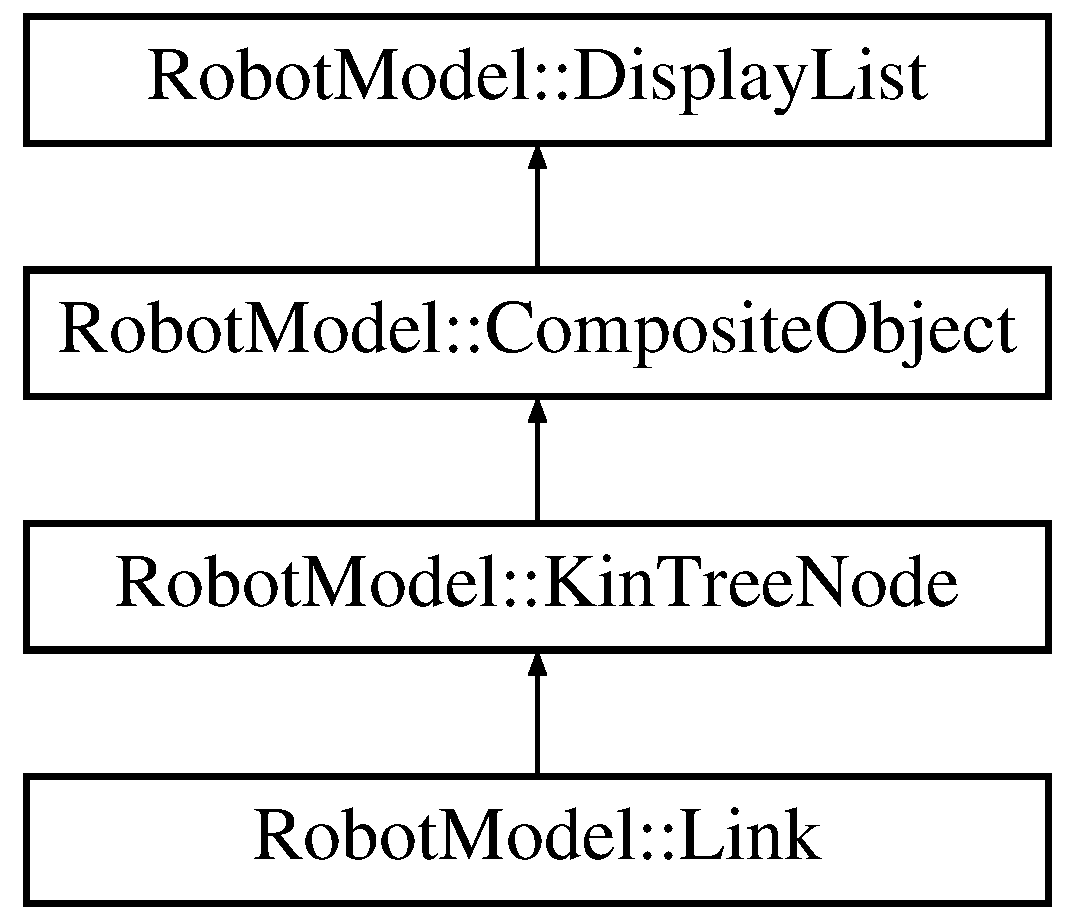
\includegraphics[height=1.8617cm]{class_robot_model_1_1_link}
\end{center}
\end{figure}
\subsection*{Public Member Functions}
\begin{DoxyCompactItemize}
\item 
\hyperlink{class_robot_model_1_1_link_adf46ff7e38787594ac9941a478083f21}{Link} (\hyperlink{class_robot_model_1_1_robot}{Robot} $\ast$robot, \hyperlink{class_robot_model_1_1_kin_tree_node}{KinTreeNode} $\ast$parent)
\item 
\hyperlink{class_robot_model_1_1_link_a666e442abb3122fe5eb1705f1b2d650d}{$\sim$Link} ()
\item 
\hyperlink{class_robot_model_1_1_link_a51f1c1b6b739dac1ecdff9e803db2499}{Link} (\hyperlink{class_robot_model_1_1_robot}{Robot} $\ast$robot, \hyperlink{class_robot_model_1_1_kin_tree_node}{KinTreeNode} $\ast$parent)
\item 
\hyperlink{class_robot_model_1_1_link_a8d7151624da1aa2dc7675ab63ec29a1c}{$\sim$Link} ()
\end{DoxyCompactItemize}


\subsection{Detailed Description}
Represents a link in the robot. 

\subsection{Constructor \& Destructor Documentation}
\hypertarget{class_robot_model_1_1_link_adf46ff7e38787594ac9941a478083f21}{
\index{RobotModel::Link@{RobotModel::Link}!Link@{Link}}
\index{Link@{Link}!RobotModel::Link@{RobotModel::Link}}
\subsubsection[{Link}]{\setlength{\rightskip}{0pt plus 5cm}Link::Link ({\bf Robot} $\ast$ {\em robot}, \/  {\bf KinTreeNode} $\ast$ {\em parent})}}
\label{class_robot_model_1_1_link_adf46ff7e38787594ac9941a478083f21}
\hypertarget{class_robot_model_1_1_link_a666e442abb3122fe5eb1705f1b2d650d}{
\index{RobotModel::Link@{RobotModel::Link}!$\sim$Link@{$\sim$Link}}
\index{$\sim$Link@{$\sim$Link}!RobotModel::Link@{RobotModel::Link}}
\subsubsection[{$\sim$Link}]{\setlength{\rightskip}{0pt plus 5cm}Link::$\sim$Link ()}}
\label{class_robot_model_1_1_link_a666e442abb3122fe5eb1705f1b2d650d}
\hypertarget{class_robot_model_1_1_link_a51f1c1b6b739dac1ecdff9e803db2499}{
\index{RobotModel::Link@{RobotModel::Link}!Link@{Link}}
\index{Link@{Link}!RobotModel::Link@{RobotModel::Link}}
\subsubsection[{Link}]{\setlength{\rightskip}{0pt plus 5cm}RobotModel::Link::Link ({\bf Robot} $\ast$ {\em robot}, \/  {\bf KinTreeNode} $\ast$ {\em parent})}}
\label{class_robot_model_1_1_link_a51f1c1b6b739dac1ecdff9e803db2499}
\hypertarget{class_robot_model_1_1_link_a8d7151624da1aa2dc7675ab63ec29a1c}{
\index{RobotModel::Link@{RobotModel::Link}!$\sim$Link@{$\sim$Link}}
\index{$\sim$Link@{$\sim$Link}!RobotModel::Link@{RobotModel::Link}}
\subsubsection[{$\sim$Link}]{\setlength{\rightskip}{0pt plus 5cm}RobotModel::Link::$\sim$Link ()}}
\label{class_robot_model_1_1_link_a8d7151624da1aa2dc7675ab63ec29a1c}


The documentation for this class was generated from the following files:\begin{DoxyCompactItemize}
\item 
/Users/kail/imClever/dev/virtualSkin/include/robotModel/\hyperlink{include_2robot_model_2link_8h}{link.h}\item 
/Users/kail/imClever/dev/virtualSkin/src/robotModel/\hyperlink{src_2robot_model_2link_8h}{link.h}\item 
/Users/kail/imClever/dev/virtualSkin/src/robotModel/\hyperlink{link_8cpp}{link.cpp}\end{DoxyCompactItemize}

\hypertarget{class_robot_model_1_1_motor}{
\section{RobotModel::Motor Class Reference}
\label{class_robot_model_1_1_motor}\index{RobotModel::Motor@{RobotModel::Motor}}
}


Affords control of one or more joints (see Branch and \hyperlink{class_robot_model_1_1_joint}{Joint}).  


{\ttfamily \#include $<$motor.h$>$}\subsection*{Public Member Functions}
\begin{DoxyCompactItemize}
\item 
\hyperlink{class_robot_model_1_1_motor_afa8d3bb8b2ad45bdc8064efa0052dd04}{Motor} (\hyperlink{class_robot_model_1_1_robot}{Robot} $\ast$robot, \hyperlink{class_robot_model_1_1_motor}{Motor} $\ast$motor=0)
\item 
\hyperlink{class_robot_model_1_1_motor_a2e57c7b2681efea1d3b7f253ee88ecd4}{$\sim$Motor} ()
\item 
const QString \& \hyperlink{class_robot_model_1_1_motor_a35eeb7f97a9339ee23c0689af2463c17}{name} () const 
\item 
\hyperlink{class_robot_model_1_1_motor}{Motor} $\ast$ \hyperlink{class_robot_model_1_1_motor_a31de5801eb1a089723a7f6980baff4a2}{parent} () const 
\item 
qreal \hyperlink{class_robot_model_1_1_motor_af2cc406d7443e2cf350408d12b8e544b}{minPos} () const 
\item 
qreal \hyperlink{class_robot_model_1_1_motor_abd6baf3a9ae74dcf970663e5ee303131}{maxPos} () const 
\item 
qreal \hyperlink{class_robot_model_1_1_motor_a8f95b65d6bf72038a4aca3a394609354}{encPos} () const 
\item 
qreal \hyperlink{class_robot_model_1_1_motor_a99de4f0e475ec8bea35fa3977fa8731f}{normPos} () const 
\item 
void \hyperlink{class_robot_model_1_1_motor_a35ae467be2d96ea6acca0860e5bda22f}{print} ()
\item 
void \hyperlink{class_robot_model_1_1_motor_a9efaa43179205b53df370f7811023eb6}{setName} (const QString \&name)
\item 
void \hyperlink{class_robot_model_1_1_motor_a404e359dac5e3af43860948d9e35f725}{setMin} (qreal)
\item 
void \hyperlink{class_robot_model_1_1_motor_ad52f8d0e1aa0b5f60b388188147a1ded}{setMax} (qreal)
\item 
void \hyperlink{class_robot_model_1_1_motor_a80d5a42cb4cc119afe0bdd4ed90a4152}{setEncPos} (qreal)
\item 
void \hyperlink{class_robot_model_1_1_motor_a2467c521c141e2cc9cf21d85d56dd20b}{setHomePos} (qreal)
\item 
void \hyperlink{class_robot_model_1_1_motor_a2c26ea7475deaef6e1546edbadf88729}{setNormPos} (qreal)
\item 
void \hyperlink{class_robot_model_1_1_motor_ae8e0845a9284fbf8013137bf6b1f9293}{home} ()
\end{DoxyCompactItemize}


\subsection{Detailed Description}
Affords control of one or more joints (see Branch and \hyperlink{class_robot_model_1_1_joint}{Joint}). This class can control an arbitrary number of joints via a linear mapping between the motor position and each joint position. The mapping is implicitly defined by the intervals motor.limits and joint.limits, and it works as follows: The motor position is set and stored in motor.encoderPosition. Using the interval motor.limits, the encoder position is normalized to a value on the interval \mbox{[}0,1\mbox{]} and this value is stored in motor.normalPosition. Finally, the normalized motor position is used to interpolate the limits of each joint to which the motor is bound. The motor object inherits QVector$<$Joint$\ast$$>$, and in this way it is its own list of joints. When a motor position is set, it immediately sets all relevent joint positions. 

\subsection{Constructor \& Destructor Documentation}
\hypertarget{class_robot_model_1_1_motor_afa8d3bb8b2ad45bdc8064efa0052dd04}{
\index{RobotModel::Motor@{RobotModel::Motor}!Motor@{Motor}}
\index{Motor@{Motor}!RobotModel::Motor@{RobotModel::Motor}}
\subsubsection[{Motor}]{\setlength{\rightskip}{0pt plus 5cm}Motor::Motor ({\bf Robot} $\ast$ {\em robot}, \/  {\bf Motor} $\ast$ {\em motor} = {\ttfamily 0})}}
\label{class_robot_model_1_1_motor_afa8d3bb8b2ad45bdc8064efa0052dd04}
\hypertarget{class_robot_model_1_1_motor_a2e57c7b2681efea1d3b7f253ee88ecd4}{
\index{RobotModel::Motor@{RobotModel::Motor}!$\sim$Motor@{$\sim$Motor}}
\index{$\sim$Motor@{$\sim$Motor}!RobotModel::Motor@{RobotModel::Motor}}
\subsubsection[{$\sim$Motor}]{\setlength{\rightskip}{0pt plus 5cm}Motor::$\sim$Motor ()}}
\label{class_robot_model_1_1_motor_a2e57c7b2681efea1d3b7f253ee88ecd4}


\subsection{Member Function Documentation}
\hypertarget{class_robot_model_1_1_motor_a8f95b65d6bf72038a4aca3a394609354}{
\index{RobotModel::Motor@{RobotModel::Motor}!encPos@{encPos}}
\index{encPos@{encPos}!RobotModel::Motor@{RobotModel::Motor}}
\subsubsection[{encPos}]{\setlength{\rightskip}{0pt plus 5cm}qreal RobotModel::Motor::encPos () const\hspace{0.3cm}{\ttfamily  \mbox{[}inline\mbox{]}}}}
\label{class_robot_model_1_1_motor_a8f95b65d6bf72038a4aca3a394609354}
\hypertarget{class_robot_model_1_1_motor_ae8e0845a9284fbf8013137bf6b1f9293}{
\index{RobotModel::Motor@{RobotModel::Motor}!home@{home}}
\index{home@{home}!RobotModel::Motor@{RobotModel::Motor}}
\subsubsection[{home}]{\setlength{\rightskip}{0pt plus 5cm}void Motor::home ()}}
\label{class_robot_model_1_1_motor_ae8e0845a9284fbf8013137bf6b1f9293}
\hypertarget{class_robot_model_1_1_motor_abd6baf3a9ae74dcf970663e5ee303131}{
\index{RobotModel::Motor@{RobotModel::Motor}!maxPos@{maxPos}}
\index{maxPos@{maxPos}!RobotModel::Motor@{RobotModel::Motor}}
\subsubsection[{maxPos}]{\setlength{\rightskip}{0pt plus 5cm}qreal RobotModel::Motor::maxPos () const\hspace{0.3cm}{\ttfamily  \mbox{[}inline\mbox{]}}}}
\label{class_robot_model_1_1_motor_abd6baf3a9ae74dcf970663e5ee303131}
\hypertarget{class_robot_model_1_1_motor_af2cc406d7443e2cf350408d12b8e544b}{
\index{RobotModel::Motor@{RobotModel::Motor}!minPos@{minPos}}
\index{minPos@{minPos}!RobotModel::Motor@{RobotModel::Motor}}
\subsubsection[{minPos}]{\setlength{\rightskip}{0pt plus 5cm}qreal RobotModel::Motor::minPos () const\hspace{0.3cm}{\ttfamily  \mbox{[}inline\mbox{]}}}}
\label{class_robot_model_1_1_motor_af2cc406d7443e2cf350408d12b8e544b}
\hypertarget{class_robot_model_1_1_motor_a35eeb7f97a9339ee23c0689af2463c17}{
\index{RobotModel::Motor@{RobotModel::Motor}!name@{name}}
\index{name@{name}!RobotModel::Motor@{RobotModel::Motor}}
\subsubsection[{name}]{\setlength{\rightskip}{0pt plus 5cm}const QString\& RobotModel::Motor::name () const\hspace{0.3cm}{\ttfamily  \mbox{[}inline\mbox{]}}}}
\label{class_robot_model_1_1_motor_a35eeb7f97a9339ee23c0689af2463c17}
\hypertarget{class_robot_model_1_1_motor_a99de4f0e475ec8bea35fa3977fa8731f}{
\index{RobotModel::Motor@{RobotModel::Motor}!normPos@{normPos}}
\index{normPos@{normPos}!RobotModel::Motor@{RobotModel::Motor}}
\subsubsection[{normPos}]{\setlength{\rightskip}{0pt plus 5cm}qreal RobotModel::Motor::normPos () const\hspace{0.3cm}{\ttfamily  \mbox{[}inline\mbox{]}}}}
\label{class_robot_model_1_1_motor_a99de4f0e475ec8bea35fa3977fa8731f}
\hypertarget{class_robot_model_1_1_motor_a31de5801eb1a089723a7f6980baff4a2}{
\index{RobotModel::Motor@{RobotModel::Motor}!parent@{parent}}
\index{parent@{parent}!RobotModel::Motor@{RobotModel::Motor}}
\subsubsection[{parent}]{\setlength{\rightskip}{0pt plus 5cm}{\bf Motor}$\ast$ RobotModel::Motor::parent () const\hspace{0.3cm}{\ttfamily  \mbox{[}inline\mbox{]}}}}
\label{class_robot_model_1_1_motor_a31de5801eb1a089723a7f6980baff4a2}
\hypertarget{class_robot_model_1_1_motor_a35ae467be2d96ea6acca0860e5bda22f}{
\index{RobotModel::Motor@{RobotModel::Motor}!print@{print}}
\index{print@{print}!RobotModel::Motor@{RobotModel::Motor}}
\subsubsection[{print}]{\setlength{\rightskip}{0pt plus 5cm}void Motor::print ()}}
\label{class_robot_model_1_1_motor_a35ae467be2d96ea6acca0860e5bda22f}
\hypertarget{class_robot_model_1_1_motor_a80d5a42cb4cc119afe0bdd4ed90a4152}{
\index{RobotModel::Motor@{RobotModel::Motor}!setEncPos@{setEncPos}}
\index{setEncPos@{setEncPos}!RobotModel::Motor@{RobotModel::Motor}}
\subsubsection[{setEncPos}]{\setlength{\rightskip}{0pt plus 5cm}void Motor::setEncPos (qreal {\em pos})}}
\label{class_robot_model_1_1_motor_a80d5a42cb4cc119afe0bdd4ed90a4152}
\hypertarget{class_robot_model_1_1_motor_a2467c521c141e2cc9cf21d85d56dd20b}{
\index{RobotModel::Motor@{RobotModel::Motor}!setHomePos@{setHomePos}}
\index{setHomePos@{setHomePos}!RobotModel::Motor@{RobotModel::Motor}}
\subsubsection[{setHomePos}]{\setlength{\rightskip}{0pt plus 5cm}void Motor::setHomePos (qreal {\em pos})}}
\label{class_robot_model_1_1_motor_a2467c521c141e2cc9cf21d85d56dd20b}
\hypertarget{class_robot_model_1_1_motor_ad52f8d0e1aa0b5f60b388188147a1ded}{
\index{RobotModel::Motor@{RobotModel::Motor}!setMax@{setMax}}
\index{setMax@{setMax}!RobotModel::Motor@{RobotModel::Motor}}
\subsubsection[{setMax}]{\setlength{\rightskip}{0pt plus 5cm}void Motor::setMax (qreal {\em max})}}
\label{class_robot_model_1_1_motor_ad52f8d0e1aa0b5f60b388188147a1ded}
\hypertarget{class_robot_model_1_1_motor_a404e359dac5e3af43860948d9e35f725}{
\index{RobotModel::Motor@{RobotModel::Motor}!setMin@{setMin}}
\index{setMin@{setMin}!RobotModel::Motor@{RobotModel::Motor}}
\subsubsection[{setMin}]{\setlength{\rightskip}{0pt plus 5cm}void Motor::setMin (qreal {\em min})}}
\label{class_robot_model_1_1_motor_a404e359dac5e3af43860948d9e35f725}
\hypertarget{class_robot_model_1_1_motor_a9efaa43179205b53df370f7811023eb6}{
\index{RobotModel::Motor@{RobotModel::Motor}!setName@{setName}}
\index{setName@{setName}!RobotModel::Motor@{RobotModel::Motor}}
\subsubsection[{setName}]{\setlength{\rightskip}{0pt plus 5cm}void RobotModel::Motor::setName (const QString \& {\em name})\hspace{0.3cm}{\ttfamily  \mbox{[}inline\mbox{]}}}}
\label{class_robot_model_1_1_motor_a9efaa43179205b53df370f7811023eb6}
\hypertarget{class_robot_model_1_1_motor_a2c26ea7475deaef6e1546edbadf88729}{
\index{RobotModel::Motor@{RobotModel::Motor}!setNormPos@{setNormPos}}
\index{setNormPos@{setNormPos}!RobotModel::Motor@{RobotModel::Motor}}
\subsubsection[{setNormPos}]{\setlength{\rightskip}{0pt plus 5cm}void Motor::setNormPos (qreal {\em pos})}}
\label{class_robot_model_1_1_motor_a2c26ea7475deaef6e1546edbadf88729}


The documentation for this class was generated from the following files:\begin{DoxyCompactItemize}
\item 
/Users/kail/imClever/dev/virtualSkin/src/robotModel/\hyperlink{motor_8h}{motor.h}\item 
/Users/kail/imClever/dev/virtualSkin/src/robotModel/\hyperlink{motor_8cpp}{motor.cpp}\end{DoxyCompactItemize}

\hypertarget{class_part_babbler}{
\section{PartBabbler Class Reference}
\label{class_part_babbler}\index{PartBabbler@{PartBabbler}}
}


Facilitates Motor Babbling.  


{\ttfamily \#include $<$partBabbler.h$>$}\subsection*{Public Member Functions}
\begin{DoxyCompactItemize}
\item 
\hyperlink{class_part_babbler_adfba4a1da8c68ba88d3451b043bb8a05}{PartBabbler} ()
\item 
\hyperlink{class_part_babbler_a64204448180c922a7928f9450f2fa38a}{$\sim$PartBabbler} ()
\item 
bool \hyperlink{class_part_babbler_a9a1ff8917964eab2e95711dd9e0594e8}{open} (const char $\ast$robotName, const char $\ast$partName)
\item 
void \hyperlink{class_part_babbler_a156d8ef91d4f8d4dfe02f9d8982c5d06}{crackBaby} (qreal velocity, bool hands)
\item 
void \hyperlink{class_part_babbler_a16e6e6a7582a5fb5903604691de52070}{doTheRobot} (qreal velocity, bool hands)
\item 
bool \hyperlink{class_part_babbler_ac62a972e85492eaaa8cfc7dcd1c9488c}{checkMotionDone} (bool $\ast$flag)
\end{DoxyCompactItemize}


\subsection{Detailed Description}
Facilitates Motor Babbling. 

\subsection{Constructor \& Destructor Documentation}
\hypertarget{class_part_babbler_adfba4a1da8c68ba88d3451b043bb8a05}{
\index{PartBabbler@{PartBabbler}!PartBabbler@{PartBabbler}}
\index{PartBabbler@{PartBabbler}!PartBabbler@{PartBabbler}}
\subsubsection[{PartBabbler}]{\setlength{\rightskip}{0pt plus 5cm}PartBabbler::PartBabbler ()}}
\label{class_part_babbler_adfba4a1da8c68ba88d3451b043bb8a05}
\hypertarget{class_part_babbler_a64204448180c922a7928f9450f2fa38a}{
\index{PartBabbler@{PartBabbler}!$\sim$PartBabbler@{$\sim$PartBabbler}}
\index{$\sim$PartBabbler@{$\sim$PartBabbler}!PartBabbler@{PartBabbler}}
\subsubsection[{$\sim$PartBabbler}]{\setlength{\rightskip}{0pt plus 5cm}PartBabbler::$\sim$PartBabbler ()}}
\label{class_part_babbler_a64204448180c922a7928f9450f2fa38a}


\subsection{Member Function Documentation}
\hypertarget{class_part_babbler_ac62a972e85492eaaa8cfc7dcd1c9488c}{
\index{PartBabbler@{PartBabbler}!checkMotionDone@{checkMotionDone}}
\index{checkMotionDone@{checkMotionDone}!PartBabbler@{PartBabbler}}
\subsubsection[{checkMotionDone}]{\setlength{\rightskip}{0pt plus 5cm}bool PartBabbler::checkMotionDone (bool $\ast$ {\em flag})\hspace{0.3cm}{\ttfamily  \mbox{[}inline\mbox{]}}}}
\label{class_part_babbler_ac62a972e85492eaaa8cfc7dcd1c9488c}
\hypertarget{class_part_babbler_a156d8ef91d4f8d4dfe02f9d8982c5d06}{
\index{PartBabbler@{PartBabbler}!crackBaby@{crackBaby}}
\index{crackBaby@{crackBaby}!PartBabbler@{PartBabbler}}
\subsubsection[{crackBaby}]{\setlength{\rightskip}{0pt plus 5cm}void PartBabbler::crackBaby (qreal {\em velocity}, \/  bool {\em hands})}}
\label{class_part_babbler_a156d8ef91d4f8d4dfe02f9d8982c5d06}
\hypertarget{class_part_babbler_a16e6e6a7582a5fb5903604691de52070}{
\index{PartBabbler@{PartBabbler}!doTheRobot@{doTheRobot}}
\index{doTheRobot@{doTheRobot}!PartBabbler@{PartBabbler}}
\subsubsection[{doTheRobot}]{\setlength{\rightskip}{0pt plus 5cm}void PartBabbler::doTheRobot (qreal {\em velocity}, \/  bool {\em hands})}}
\label{class_part_babbler_a16e6e6a7582a5fb5903604691de52070}
\hypertarget{class_part_babbler_a9a1ff8917964eab2e95711dd9e0594e8}{
\index{PartBabbler@{PartBabbler}!open@{open}}
\index{open@{open}!PartBabbler@{PartBabbler}}
\subsubsection[{open}]{\setlength{\rightskip}{0pt plus 5cm}bool PartBabbler::open (const char $\ast$ {\em robotName}, \/  const char $\ast$ {\em partName})\hspace{0.3cm}{\ttfamily  \mbox{[}inline\mbox{]}}}}
\label{class_part_babbler_a9a1ff8917964eab2e95711dd9e0594e8}


The documentation for this class was generated from the following files:\begin{DoxyCompactItemize}
\item 
/Users/kail/imClever/dev/virtualSkin/src/iCubBabbler/\hyperlink{part_babbler_8h}{partBabbler.h}\item 
/Users/kail/imClever/dev/virtualSkin/src/iCubBabbler/\hyperlink{part_babbler_8cpp}{partBabbler.cpp}\end{DoxyCompactItemize}

\hypertarget{class_robot_model_1_1_part_controller}{
\section{RobotModel::PartController Class Reference}
\label{class_robot_model_1_1_part_controller}\index{RobotModel::PartController@{RobotModel::PartController}}
}


Provides a remote device driver for a YARP port This could be a motor control interface for one part of the iCub for example. see: \href{http://eris.liralab.it/wiki/Motor_control.}{\tt http://eris.liralab.it/wiki/Motor\_\-control.}  


{\ttfamily \#include $<$partController.h$>$}\subsection*{Public Member Functions}
\begin{DoxyCompactItemize}
\item 
\hyperlink{class_robot_model_1_1_part_controller_a9e5274fba78804eb936fc84048f21e73}{PartController} ()
\item 
\hyperlink{class_robot_model_1_1_part_controller_aee568c7268577894104e0739a99c33f5}{$\sim$PartController} ()
\item 
bool \hyperlink{class_robot_model_1_1_part_controller_a20331379a94c33ef330792e6b9e8b94f}{open} (const char $\ast$\_\-robotName, const char $\ast$\_\-partName)
\item 
void \hyperlink{class_robot_model_1_1_part_controller_a7e0fbd5bd25cebb78cd1b095c2055dac}{close} ()
\item 
bool \hyperlink{class_robot_model_1_1_part_controller_a02d325bdc7bd18023e47f97894a2de49}{isValid} ()
\item 
int \hyperlink{class_robot_model_1_1_part_controller_a2fb04bfb6b1da63201fdaf3dac6591dc}{getNumJoints} ()
\item 
bool \hyperlink{class_robot_model_1_1_part_controller_a4052252cc91ea1387d5a33c968e9a84a}{checkMotionDone} (bool $\ast$)
\item 
bool \hyperlink{class_robot_model_1_1_part_controller_aeb479f7ffd70c0cf80beabf38b1073f7}{stop} ()
\item 
bool \hyperlink{class_robot_model_1_1_part_controller_a3082aaf9c98045fb3309dcaef6416fbe}{setRefSpeeds} (const qreal)
\item 
bool \hyperlink{class_robot_model_1_1_part_controller_a5481c9f2cbbd8370fd2e5b62c38c7d2f}{setRefSpeeds} (const QVector$<$ qreal $>$ \&speeds)
\item 
bool \hyperlink{class_robot_model_1_1_part_controller_aeb2bca8add9b083ebd19d0d2d07fdfd4}{positionMove} (const QVector$<$ qreal $>$ \&)
\item 
bool \hyperlink{class_robot_model_1_1_part_controller_ac5476493b51412c7b6008cf58111543b}{velocityMove} (int i, qreal v)
\item 
bool \hyperlink{class_robot_model_1_1_part_controller_af513e2aa6934bcfeef7d2bf73e9b3cc3}{randomPosMove} (qreal maxSpeed, bool hands)
\item 
\hyperlink{class_robot_model_1_1_part_controller_aa710415b09f5e55af5be9518926c427e}{PartController} ()
\item 
\hyperlink{class_robot_model_1_1_part_controller_a3af4c72e4e237805328951a0b4392a46}{$\sim$PartController} ()
\item 
bool \hyperlink{class_robot_model_1_1_part_controller_ad7344d850243e282749bd9fa5f84df5c}{open} (const char $\ast$\_\-robotName, const char $\ast$\_\-partName)
\item 
void \hyperlink{class_robot_model_1_1_part_controller_a2042c9595ee1dd1e87f0095bc10cc2be}{close} ()
\item 
bool \hyperlink{class_robot_model_1_1_part_controller_a03d04564ed45e8f991075a059a5d557f}{isValid} ()
\item 
int \hyperlink{class_robot_model_1_1_part_controller_a2fb04bfb6b1da63201fdaf3dac6591dc}{getNumJoints} ()
\item 
bool \hyperlink{class_robot_model_1_1_part_controller_aeebcb6a50ff927c552f6e41cc355902b}{checkMotionDone} (bool $\ast$)
\item 
bool \hyperlink{class_robot_model_1_1_part_controller_aeb479f7ffd70c0cf80beabf38b1073f7}{stop} ()
\item 
bool \hyperlink{class_robot_model_1_1_part_controller_a8fda7fd0b7914ec93b349b0b11f8d757}{setRefSpeeds} (const qreal)
\item 
bool \hyperlink{class_robot_model_1_1_part_controller_a5481c9f2cbbd8370fd2e5b62c38c7d2f}{setRefSpeeds} (const QVector$<$ qreal $>$ \&speeds)
\item 
bool \hyperlink{class_robot_model_1_1_part_controller_a9ab9fab080b18fa2fe162ccedb928460}{positionMove} (const QVector$<$ qreal $>$ \&)
\item 
bool \hyperlink{class_robot_model_1_1_part_controller_a8ac6b4519903ab433a7474e0491333f3}{velocityMove} (int i, qreal v)
\item 
bool \hyperlink{class_robot_model_1_1_part_controller_aa7dfbc575182f6eeb56c4190ea0e50f7}{randomPosMove} (qreal maxSpeed, bool hands)
\end{DoxyCompactItemize}


\subsection{Detailed Description}
Provides a remote device driver for a YARP port This could be a motor control interface for one part of the iCub for example. see: \href{http://eris.liralab.it/wiki/Motor_control.}{\tt http://eris.liralab.it/wiki/Motor\_\-control.} 

\subsection{Constructor \& Destructor Documentation}
\hypertarget{class_robot_model_1_1_part_controller_a9e5274fba78804eb936fc84048f21e73}{
\index{RobotModel::PartController@{RobotModel::PartController}!PartController@{PartController}}
\index{PartController@{PartController}!RobotModel::PartController@{RobotModel::PartController}}
\subsubsection[{PartController}]{\setlength{\rightskip}{0pt plus 5cm}PartController::PartController ()}}
\label{class_robot_model_1_1_part_controller_a9e5274fba78804eb936fc84048f21e73}
\hypertarget{class_robot_model_1_1_part_controller_aee568c7268577894104e0739a99c33f5}{
\index{RobotModel::PartController@{RobotModel::PartController}!$\sim$PartController@{$\sim$PartController}}
\index{$\sim$PartController@{$\sim$PartController}!RobotModel::PartController@{RobotModel::PartController}}
\subsubsection[{$\sim$PartController}]{\setlength{\rightskip}{0pt plus 5cm}PartController::$\sim$PartController ()}}
\label{class_robot_model_1_1_part_controller_aee568c7268577894104e0739a99c33f5}
\hypertarget{class_robot_model_1_1_part_controller_aa710415b09f5e55af5be9518926c427e}{
\index{RobotModel::PartController@{RobotModel::PartController}!PartController@{PartController}}
\index{PartController@{PartController}!RobotModel::PartController@{RobotModel::PartController}}
\subsubsection[{PartController}]{\setlength{\rightskip}{0pt plus 5cm}RobotModel::PartController::PartController ()}}
\label{class_robot_model_1_1_part_controller_aa710415b09f5e55af5be9518926c427e}
\hypertarget{class_robot_model_1_1_part_controller_a3af4c72e4e237805328951a0b4392a46}{
\index{RobotModel::PartController@{RobotModel::PartController}!$\sim$PartController@{$\sim$PartController}}
\index{$\sim$PartController@{$\sim$PartController}!RobotModel::PartController@{RobotModel::PartController}}
\subsubsection[{$\sim$PartController}]{\setlength{\rightskip}{0pt plus 5cm}RobotModel::PartController::$\sim$PartController ()}}
\label{class_robot_model_1_1_part_controller_a3af4c72e4e237805328951a0b4392a46}


\subsection{Member Function Documentation}
\hypertarget{class_robot_model_1_1_part_controller_aeebcb6a50ff927c552f6e41cc355902b}{
\index{RobotModel::PartController@{RobotModel::PartController}!checkMotionDone@{checkMotionDone}}
\index{checkMotionDone@{checkMotionDone}!RobotModel::PartController@{RobotModel::PartController}}
\subsubsection[{checkMotionDone}]{\setlength{\rightskip}{0pt plus 5cm}bool RobotModel::PartController::checkMotionDone (bool $\ast$)}}
\label{class_robot_model_1_1_part_controller_aeebcb6a50ff927c552f6e41cc355902b}
\hypertarget{class_robot_model_1_1_part_controller_a4052252cc91ea1387d5a33c968e9a84a}{
\index{RobotModel::PartController@{RobotModel::PartController}!checkMotionDone@{checkMotionDone}}
\index{checkMotionDone@{checkMotionDone}!RobotModel::PartController@{RobotModel::PartController}}
\subsubsection[{checkMotionDone}]{\setlength{\rightskip}{0pt plus 5cm}bool PartController::checkMotionDone (bool $\ast$ {\em flag})}}
\label{class_robot_model_1_1_part_controller_a4052252cc91ea1387d5a33c968e9a84a}
\hypertarget{class_robot_model_1_1_part_controller_a2042c9595ee1dd1e87f0095bc10cc2be}{
\index{RobotModel::PartController@{RobotModel::PartController}!close@{close}}
\index{close@{close}!RobotModel::PartController@{RobotModel::PartController}}
\subsubsection[{close}]{\setlength{\rightskip}{0pt plus 5cm}void RobotModel::PartController::close ()}}
\label{class_robot_model_1_1_part_controller_a2042c9595ee1dd1e87f0095bc10cc2be}
\hypertarget{class_robot_model_1_1_part_controller_a7e0fbd5bd25cebb78cd1b095c2055dac}{
\index{RobotModel::PartController@{RobotModel::PartController}!close@{close}}
\index{close@{close}!RobotModel::PartController@{RobotModel::PartController}}
\subsubsection[{close}]{\setlength{\rightskip}{0pt plus 5cm}void PartController::close ()}}
\label{class_robot_model_1_1_part_controller_a7e0fbd5bd25cebb78cd1b095c2055dac}
\hypertarget{class_robot_model_1_1_part_controller_a2fb04bfb6b1da63201fdaf3dac6591dc}{
\index{RobotModel::PartController@{RobotModel::PartController}!getNumJoints@{getNumJoints}}
\index{getNumJoints@{getNumJoints}!RobotModel::PartController@{RobotModel::PartController}}
\subsubsection[{getNumJoints}]{\setlength{\rightskip}{0pt plus 5cm}int RobotModel::PartController::getNumJoints ()\hspace{0.3cm}{\ttfamily  \mbox{[}inline\mbox{]}}}}
\label{class_robot_model_1_1_part_controller_a2fb04bfb6b1da63201fdaf3dac6591dc}
\hypertarget{class_robot_model_1_1_part_controller_a2fb04bfb6b1da63201fdaf3dac6591dc}{
\index{RobotModel::PartController@{RobotModel::PartController}!getNumJoints@{getNumJoints}}
\index{getNumJoints@{getNumJoints}!RobotModel::PartController@{RobotModel::PartController}}
\subsubsection[{getNumJoints}]{\setlength{\rightskip}{0pt plus 5cm}int RobotModel::PartController::getNumJoints ()\hspace{0.3cm}{\ttfamily  \mbox{[}inline\mbox{]}}}}
\label{class_robot_model_1_1_part_controller_a2fb04bfb6b1da63201fdaf3dac6591dc}
\hypertarget{class_robot_model_1_1_part_controller_a03d04564ed45e8f991075a059a5d557f}{
\index{RobotModel::PartController@{RobotModel::PartController}!isValid@{isValid}}
\index{isValid@{isValid}!RobotModel::PartController@{RobotModel::PartController}}
\subsubsection[{isValid}]{\setlength{\rightskip}{0pt plus 5cm}bool RobotModel::PartController::isValid ()}}
\label{class_robot_model_1_1_part_controller_a03d04564ed45e8f991075a059a5d557f}
\hypertarget{class_robot_model_1_1_part_controller_a02d325bdc7bd18023e47f97894a2de49}{
\index{RobotModel::PartController@{RobotModel::PartController}!isValid@{isValid}}
\index{isValid@{isValid}!RobotModel::PartController@{RobotModel::PartController}}
\subsubsection[{isValid}]{\setlength{\rightskip}{0pt plus 5cm}bool PartController::isValid ()}}
\label{class_robot_model_1_1_part_controller_a02d325bdc7bd18023e47f97894a2de49}
\hypertarget{class_robot_model_1_1_part_controller_ad7344d850243e282749bd9fa5f84df5c}{
\index{RobotModel::PartController@{RobotModel::PartController}!open@{open}}
\index{open@{open}!RobotModel::PartController@{RobotModel::PartController}}
\subsubsection[{open}]{\setlength{\rightskip}{0pt plus 5cm}bool RobotModel::PartController::open (const char $\ast$ {\em \_\-robotName}, \/  const char $\ast$ {\em \_\-partName})}}
\label{class_robot_model_1_1_part_controller_ad7344d850243e282749bd9fa5f84df5c}
\hypertarget{class_robot_model_1_1_part_controller_a20331379a94c33ef330792e6b9e8b94f}{
\index{RobotModel::PartController@{RobotModel::PartController}!open@{open}}
\index{open@{open}!RobotModel::PartController@{RobotModel::PartController}}
\subsubsection[{open}]{\setlength{\rightskip}{0pt plus 5cm}bool PartController::open (const char $\ast$ {\em \_\-robotName}, \/  const char $\ast$ {\em \_\-partName})}}
\label{class_robot_model_1_1_part_controller_a20331379a94c33ef330792e6b9e8b94f}
\hypertarget{class_robot_model_1_1_part_controller_a9ab9fab080b18fa2fe162ccedb928460}{
\index{RobotModel::PartController@{RobotModel::PartController}!positionMove@{positionMove}}
\index{positionMove@{positionMove}!RobotModel::PartController@{RobotModel::PartController}}
\subsubsection[{positionMove}]{\setlength{\rightskip}{0pt plus 5cm}bool RobotModel::PartController::positionMove (const QVector$<$ qreal $>$ \&)}}
\label{class_robot_model_1_1_part_controller_a9ab9fab080b18fa2fe162ccedb928460}
\hypertarget{class_robot_model_1_1_part_controller_aeb2bca8add9b083ebd19d0d2d07fdfd4}{
\index{RobotModel::PartController@{RobotModel::PartController}!positionMove@{positionMove}}
\index{positionMove@{positionMove}!RobotModel::PartController@{RobotModel::PartController}}
\subsubsection[{positionMove}]{\setlength{\rightskip}{0pt plus 5cm}bool PartController::positionMove (const QVector$<$ qreal $>$ \& {\em positions})}}
\label{class_robot_model_1_1_part_controller_aeb2bca8add9b083ebd19d0d2d07fdfd4}
\hypertarget{class_robot_model_1_1_part_controller_aa7dfbc575182f6eeb56c4190ea0e50f7}{
\index{RobotModel::PartController@{RobotModel::PartController}!randomPosMove@{randomPosMove}}
\index{randomPosMove@{randomPosMove}!RobotModel::PartController@{RobotModel::PartController}}
\subsubsection[{randomPosMove}]{\setlength{\rightskip}{0pt plus 5cm}bool RobotModel::PartController::randomPosMove (qreal {\em maxSpeed}, \/  bool {\em hands})}}
\label{class_robot_model_1_1_part_controller_aa7dfbc575182f6eeb56c4190ea0e50f7}
\hypertarget{class_robot_model_1_1_part_controller_af513e2aa6934bcfeef7d2bf73e9b3cc3}{
\index{RobotModel::PartController@{RobotModel::PartController}!randomPosMove@{randomPosMove}}
\index{randomPosMove@{randomPosMove}!RobotModel::PartController@{RobotModel::PartController}}
\subsubsection[{randomPosMove}]{\setlength{\rightskip}{0pt plus 5cm}bool PartController::randomPosMove (qreal {\em maxSpeed}, \/  bool {\em hands})}}
\label{class_robot_model_1_1_part_controller_af513e2aa6934bcfeef7d2bf73e9b3cc3}
\hypertarget{class_robot_model_1_1_part_controller_a5481c9f2cbbd8370fd2e5b62c38c7d2f}{
\index{RobotModel::PartController@{RobotModel::PartController}!setRefSpeeds@{setRefSpeeds}}
\index{setRefSpeeds@{setRefSpeeds}!RobotModel::PartController@{RobotModel::PartController}}
\subsubsection[{setRefSpeeds}]{\setlength{\rightskip}{0pt plus 5cm}bool RobotModel::PartController::setRefSpeeds (const QVector$<$ qreal $>$ \& {\em speeds})\hspace{0.3cm}{\ttfamily  \mbox{[}inline\mbox{]}}}}
\label{class_robot_model_1_1_part_controller_a5481c9f2cbbd8370fd2e5b62c38c7d2f}
\hypertarget{class_robot_model_1_1_part_controller_a8fda7fd0b7914ec93b349b0b11f8d757}{
\index{RobotModel::PartController@{RobotModel::PartController}!setRefSpeeds@{setRefSpeeds}}
\index{setRefSpeeds@{setRefSpeeds}!RobotModel::PartController@{RobotModel::PartController}}
\subsubsection[{setRefSpeeds}]{\setlength{\rightskip}{0pt plus 5cm}bool RobotModel::PartController::setRefSpeeds (const  {\em qreal})}}
\label{class_robot_model_1_1_part_controller_a8fda7fd0b7914ec93b349b0b11f8d757}
\hypertarget{class_robot_model_1_1_part_controller_a5481c9f2cbbd8370fd2e5b62c38c7d2f}{
\index{RobotModel::PartController@{RobotModel::PartController}!setRefSpeeds@{setRefSpeeds}}
\index{setRefSpeeds@{setRefSpeeds}!RobotModel::PartController@{RobotModel::PartController}}
\subsubsection[{setRefSpeeds}]{\setlength{\rightskip}{0pt plus 5cm}bool RobotModel::PartController::setRefSpeeds (const QVector$<$ qreal $>$ \& {\em speeds})\hspace{0.3cm}{\ttfamily  \mbox{[}inline\mbox{]}}}}
\label{class_robot_model_1_1_part_controller_a5481c9f2cbbd8370fd2e5b62c38c7d2f}
\hypertarget{class_robot_model_1_1_part_controller_a3082aaf9c98045fb3309dcaef6416fbe}{
\index{RobotModel::PartController@{RobotModel::PartController}!setRefSpeeds@{setRefSpeeds}}
\index{setRefSpeeds@{setRefSpeeds}!RobotModel::PartController@{RobotModel::PartController}}
\subsubsection[{setRefSpeeds}]{\setlength{\rightskip}{0pt plus 5cm}bool PartController::setRefSpeeds (const qreal {\em speed})}}
\label{class_robot_model_1_1_part_controller_a3082aaf9c98045fb3309dcaef6416fbe}
\hypertarget{class_robot_model_1_1_part_controller_aeb479f7ffd70c0cf80beabf38b1073f7}{
\index{RobotModel::PartController@{RobotModel::PartController}!stop@{stop}}
\index{stop@{stop}!RobotModel::PartController@{RobotModel::PartController}}
\subsubsection[{stop}]{\setlength{\rightskip}{0pt plus 5cm}bool RobotModel::PartController::stop ()\hspace{0.3cm}{\ttfamily  \mbox{[}inline\mbox{]}}}}
\label{class_robot_model_1_1_part_controller_aeb479f7ffd70c0cf80beabf38b1073f7}
\hypertarget{class_robot_model_1_1_part_controller_aeb479f7ffd70c0cf80beabf38b1073f7}{
\index{RobotModel::PartController@{RobotModel::PartController}!stop@{stop}}
\index{stop@{stop}!RobotModel::PartController@{RobotModel::PartController}}
\subsubsection[{stop}]{\setlength{\rightskip}{0pt plus 5cm}bool RobotModel::PartController::stop ()\hspace{0.3cm}{\ttfamily  \mbox{[}inline\mbox{]}}}}
\label{class_robot_model_1_1_part_controller_aeb479f7ffd70c0cf80beabf38b1073f7}
\hypertarget{class_robot_model_1_1_part_controller_a8ac6b4519903ab433a7474e0491333f3}{
\index{RobotModel::PartController@{RobotModel::PartController}!velocityMove@{velocityMove}}
\index{velocityMove@{velocityMove}!RobotModel::PartController@{RobotModel::PartController}}
\subsubsection[{velocityMove}]{\setlength{\rightskip}{0pt plus 5cm}bool RobotModel::PartController::velocityMove (int {\em i}, \/  qreal {\em v})}}
\label{class_robot_model_1_1_part_controller_a8ac6b4519903ab433a7474e0491333f3}
\hypertarget{class_robot_model_1_1_part_controller_ac5476493b51412c7b6008cf58111543b}{
\index{RobotModel::PartController@{RobotModel::PartController}!velocityMove@{velocityMove}}
\index{velocityMove@{velocityMove}!RobotModel::PartController@{RobotModel::PartController}}
\subsubsection[{velocityMove}]{\setlength{\rightskip}{0pt plus 5cm}bool PartController::velocityMove (int {\em i}, \/  qreal {\em v})}}
\label{class_robot_model_1_1_part_controller_ac5476493b51412c7b6008cf58111543b}


The documentation for this class was generated from the following files:\begin{DoxyCompactItemize}
\item 
/Users/kail/imClever/dev/virtualSkin/include/yarpUtil/\hyperlink{include_2yarp_util_2part_controller_8h}{partController.h}\item 
/Users/kail/imClever/dev/virtualSkin/src/yarpUtil/\hyperlink{src_2yarp_util_2part_controller_8h}{partController.h}\item 
/Users/kail/imClever/dev/virtualSkin/src/yarpUtil/\hyperlink{part_controller_8cpp}{partController.cpp}\end{DoxyCompactItemize}

\hypertarget{class_robot_model_1_1_primitive_object}{
\section{RobotModel::PrimitiveObject Class Reference}
\label{class_robot_model_1_1_primitive_object}\index{RobotModel::PrimitiveObject@{RobotModel::PrimitiveObject}}
}


{\ttfamily \#include $<$primitiveobject.h$>$}Inheritance diagram for RobotModel::PrimitiveObject::\begin{figure}[H]
\begin{center}
\leavevmode
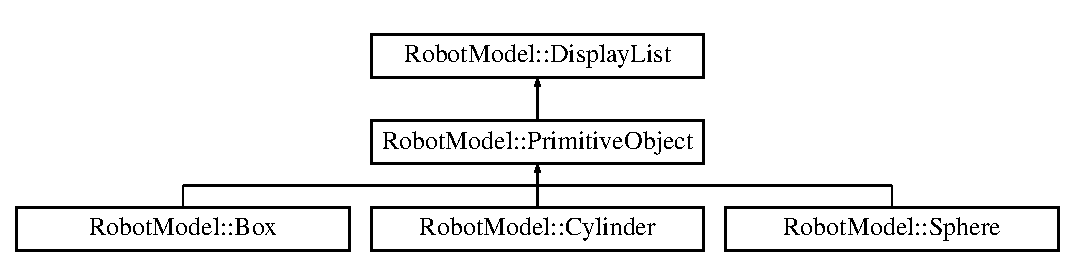
\includegraphics[height=1.57303cm]{class_robot_model_1_1_primitive_object}
\end{center}
\end{figure}
\subsection*{Public Member Functions}
\begin{DoxyCompactItemize}
\item 
\hyperlink{class_robot_model_1_1_primitive_object_ad8db4622c9ec75d92c70f4fba00863bf}{PrimitiveObject} ()
\item 
virtual \hyperlink{class_robot_model_1_1_primitive_object_a30e56bb8d777bf91ec7627fdfa0073b2}{$\sim$PrimitiveObject} ()
\item 
void \hyperlink{class_robot_model_1_1_primitive_object_a61c7cffdac933e1f363fa7d4715f669c}{setName} (const QString \&aName)
\item 
const QString \& \hyperlink{class_robot_model_1_1_primitive_object_a2bad14bd18e70f3e95b6ebfca7014d2e}{getName} ()
\item 
void \hyperlink{class_robot_model_1_1_primitive_object_afdcf8007d5aebfa88356d5551afb9775}{setParent} (\hyperlink{class_robot_model_1_1_composite_object}{CompositeObject} $\ast$object)
\item 
\hyperlink{class_robot_model_1_1_composite_object}{CompositeObject} $\ast$ \hyperlink{class_robot_model_1_1_primitive_object_a6981588496b77d1942435296631d1ef0}{getParent} ()
\item 
void \hyperlink{class_robot_model_1_1_primitive_object_a2d5bb08b04bf39964106c981cdca7d0e}{setL} (const QMatrix4x4 \&txfr)
\item 
void \hyperlink{class_robot_model_1_1_primitive_object_ac87b33448b7e82dddbca79f57ea8cbb5}{update} (const QMatrix4x4 \&txfr)
\item 
void \hyperlink{class_robot_model_1_1_primitive_object_a0a7cfefb126e4f37c208c516f8ffd9bb}{setCartesianRotation} (const QVector3D \&rot)
\item 
void \hyperlink{class_robot_model_1_1_primitive_object_a69c30287deb6549fbde68d1ba37424a8}{cartesianRotate} (const QVector3D \&rot)
\item 
void \hyperlink{class_robot_model_1_1_primitive_object_a3ae3782ae64f5fc07f4d18646e04ed21}{setAxisAngleRotation} (const QVector3D \&axis, qreal angle)
\item 
void \hyperlink{class_robot_model_1_1_primitive_object_a97b449302680b96410ff7296c794f640}{axisAngleRotate} (const QVector3D \&axis, qreal angle)
\item 
void \hyperlink{class_robot_model_1_1_primitive_object_a07ece283ed8f0f0e3cdf6f36ac7b34dd}{specialRotate} (const QVector3D \&axis, qreal angle=0)
\item 
void \hyperlink{class_robot_model_1_1_primitive_object_ae6c417003b52df18a52711031e95c44a}{setTranslation} (const QVector3D \&trans)
\item 
void \hyperlink{class_robot_model_1_1_primitive_object_ae41a1dcacd77b59c44409a77b0183a77}{translate} (const QVector3D \&trans)
\item 
\hyperlink{class_robot_model_1_1_primitive_object_a93382341d2ad150badc6b28300e8047b}{PrimitiveObject} ()
\item 
virtual \hyperlink{class_robot_model_1_1_primitive_object_aaa5d9d16c5eb4122376afc32ad9fd3d8}{$\sim$PrimitiveObject} ()
\item 
void \hyperlink{class_robot_model_1_1_primitive_object_a61c7cffdac933e1f363fa7d4715f669c}{setName} (const QString \&aName)
\item 
const QString \& \hyperlink{class_robot_model_1_1_primitive_object_a2bad14bd18e70f3e95b6ebfca7014d2e}{getName} ()
\item 
void \hyperlink{class_robot_model_1_1_primitive_object_a9097dd663246a16af3da8a4b193e6c14}{setParent} (\hyperlink{class_robot_model_1_1_composite_object}{CompositeObject} $\ast$object)
\item 
\hyperlink{class_robot_model_1_1_composite_object}{CompositeObject} $\ast$ \hyperlink{class_robot_model_1_1_primitive_object_a6981588496b77d1942435296631d1ef0}{getParent} ()
\item 
void \hyperlink{class_robot_model_1_1_primitive_object_a299181992bf3af3dab1a119e03b2944e}{setL} (const QMatrix4x4 \&txfr)
\item 
void \hyperlink{class_robot_model_1_1_primitive_object_ad6d1d0cfd2808ecf051a0d49689dfa86}{update} (const QMatrix4x4 \&txfr)
\item 
void \hyperlink{class_robot_model_1_1_primitive_object_afa2afdbe412aadfe4d7bb951e4d7b8fa}{setCartesianRotation} (const QVector3D \&rot)
\item 
void \hyperlink{class_robot_model_1_1_primitive_object_aa490f6642a6a02d48cf8ed9cd49a47f7}{cartesianRotate} (const QVector3D \&rot)
\item 
void \hyperlink{class_robot_model_1_1_primitive_object_a4a91537e10478b31fb8a025c0faac770}{setAxisAngleRotation} (const QVector3D \&axis, qreal angle)
\item 
void \hyperlink{class_robot_model_1_1_primitive_object_ae57db819937782138821a30960a72aa0}{axisAngleRotate} (const QVector3D \&axis, qreal angle)
\item 
void \hyperlink{class_robot_model_1_1_primitive_object_a33c01b56d7daf2e1d94419f25b9fa902}{specialRotate} (const QVector3D \&axis, qreal angle=0)
\item 
void \hyperlink{class_robot_model_1_1_primitive_object_a58f3d8655dd442ee1032f3582027604a}{setTranslation} (const QVector3D \&trans)
\item 
void \hyperlink{class_robot_model_1_1_primitive_object_aeddf2c45f6a3d60f2566e58728cc2a96}{translate} (const QVector3D \&trans)
\end{DoxyCompactItemize}
\subsection*{Protected Member Functions}
\begin{DoxyCompactItemize}
\item 
void \hyperlink{class_robot_model_1_1_primitive_object_a8fc60e9e4a29b895d45871d842081605}{doNotCollideWith} (\hyperlink{class_robot_model_1_1_composite_object}{CompositeObject} $\ast$object)
\item 
void \hyperlink{class_robot_model_1_1_primitive_object_a498038d3817c1c24ddc5b8e9ca7afdf9}{doNotCollideWith} (\hyperlink{class_robot_model_1_1_composite_object}{CompositeObject} $\ast$object)
\end{DoxyCompactItemize}
\subsection*{Protected Attributes}
\begin{DoxyCompactItemize}
\item 
QString \hyperlink{class_robot_model_1_1_primitive_object_ae14d0349fba88a7de488c28934bf38ce}{name}
\item 
\hyperlink{class_robot_model_1_1_composite_object}{CompositeObject} $\ast$ \hyperlink{class_robot_model_1_1_primitive_object_a242ae58660af2bf8f7e3354f55486c47}{parent}
\item 
DtShapeRef \hyperlink{class_robot_model_1_1_primitive_object_ac0e31de5b780652446fdaa06eeec47d6}{shape}
\item 
\hyperlink{class_robot_model_1_1_displ_matrix}{DisplMatrix} \hyperlink{class_robot_model_1_1_primitive_object_a920286d17b47f5fb033de4418f4755a5}{L}
\item 
QMutex \hyperlink{class_robot_model_1_1_primitive_object_a04f683e6cd9c4acc4bd8436cd8c52e15}{mutex}
\end{DoxyCompactItemize}


\subsection{Constructor \& Destructor Documentation}
\hypertarget{class_robot_model_1_1_primitive_object_ad8db4622c9ec75d92c70f4fba00863bf}{
\index{RobotModel::PrimitiveObject@{RobotModel::PrimitiveObject}!PrimitiveObject@{PrimitiveObject}}
\index{PrimitiveObject@{PrimitiveObject}!RobotModel::PrimitiveObject@{RobotModel::PrimitiveObject}}
\subsubsection[{PrimitiveObject}]{\setlength{\rightskip}{0pt plus 5cm}PrimitiveObject::PrimitiveObject ()}}
\label{class_robot_model_1_1_primitive_object_ad8db4622c9ec75d92c70f4fba00863bf}
\hypertarget{class_robot_model_1_1_primitive_object_a30e56bb8d777bf91ec7627fdfa0073b2}{
\index{RobotModel::PrimitiveObject@{RobotModel::PrimitiveObject}!$\sim$PrimitiveObject@{$\sim$PrimitiveObject}}
\index{$\sim$PrimitiveObject@{$\sim$PrimitiveObject}!RobotModel::PrimitiveObject@{RobotModel::PrimitiveObject}}
\subsubsection[{$\sim$PrimitiveObject}]{\setlength{\rightskip}{0pt plus 5cm}PrimitiveObject::$\sim$PrimitiveObject ()\hspace{0.3cm}{\ttfamily  \mbox{[}virtual\mbox{]}}}}
\label{class_robot_model_1_1_primitive_object_a30e56bb8d777bf91ec7627fdfa0073b2}
\hypertarget{class_robot_model_1_1_primitive_object_a93382341d2ad150badc6b28300e8047b}{
\index{RobotModel::PrimitiveObject@{RobotModel::PrimitiveObject}!PrimitiveObject@{PrimitiveObject}}
\index{PrimitiveObject@{PrimitiveObject}!RobotModel::PrimitiveObject@{RobotModel::PrimitiveObject}}
\subsubsection[{PrimitiveObject}]{\setlength{\rightskip}{0pt plus 5cm}RobotModel::PrimitiveObject::PrimitiveObject ()}}
\label{class_robot_model_1_1_primitive_object_a93382341d2ad150badc6b28300e8047b}
\hypertarget{class_robot_model_1_1_primitive_object_aaa5d9d16c5eb4122376afc32ad9fd3d8}{
\index{RobotModel::PrimitiveObject@{RobotModel::PrimitiveObject}!$\sim$PrimitiveObject@{$\sim$PrimitiveObject}}
\index{$\sim$PrimitiveObject@{$\sim$PrimitiveObject}!RobotModel::PrimitiveObject@{RobotModel::PrimitiveObject}}
\subsubsection[{$\sim$PrimitiveObject}]{\setlength{\rightskip}{0pt plus 5cm}virtual RobotModel::PrimitiveObject::$\sim$PrimitiveObject ()\hspace{0.3cm}{\ttfamily  \mbox{[}virtual\mbox{]}}}}
\label{class_robot_model_1_1_primitive_object_aaa5d9d16c5eb4122376afc32ad9fd3d8}


\subsection{Member Function Documentation}
\hypertarget{class_robot_model_1_1_primitive_object_ae57db819937782138821a30960a72aa0}{
\index{RobotModel::PrimitiveObject@{RobotModel::PrimitiveObject}!axisAngleRotate@{axisAngleRotate}}
\index{axisAngleRotate@{axisAngleRotate}!RobotModel::PrimitiveObject@{RobotModel::PrimitiveObject}}
\subsubsection[{axisAngleRotate}]{\setlength{\rightskip}{0pt plus 5cm}void RobotModel::PrimitiveObject::axisAngleRotate (const QVector3D \& {\em axis}, \/  qreal {\em angle})\hspace{0.3cm}{\ttfamily  \mbox{[}virtual\mbox{]}}}}
\label{class_robot_model_1_1_primitive_object_ae57db819937782138821a30960a72aa0}


Reimplemented from \hyperlink{class_robot_model_1_1_display_list_a9a7084168997ac285ee1e9f4041a8d57}{RobotModel::DisplayList}.\hypertarget{class_robot_model_1_1_primitive_object_a97b449302680b96410ff7296c794f640}{
\index{RobotModel::PrimitiveObject@{RobotModel::PrimitiveObject}!axisAngleRotate@{axisAngleRotate}}
\index{axisAngleRotate@{axisAngleRotate}!RobotModel::PrimitiveObject@{RobotModel::PrimitiveObject}}
\subsubsection[{axisAngleRotate}]{\setlength{\rightskip}{0pt plus 5cm}void PrimitiveObject::axisAngleRotate (const QVector3D \& {\em axis}, \/  qreal {\em angle})\hspace{0.3cm}{\ttfamily  \mbox{[}virtual\mbox{]}}}}
\label{class_robot_model_1_1_primitive_object_a97b449302680b96410ff7296c794f640}


Reimplemented from \hyperlink{class_robot_model_1_1_display_list_a9a7084168997ac285ee1e9f4041a8d57}{RobotModel::DisplayList}.\hypertarget{class_robot_model_1_1_primitive_object_aa490f6642a6a02d48cf8ed9cd49a47f7}{
\index{RobotModel::PrimitiveObject@{RobotModel::PrimitiveObject}!cartesianRotate@{cartesianRotate}}
\index{cartesianRotate@{cartesianRotate}!RobotModel::PrimitiveObject@{RobotModel::PrimitiveObject}}
\subsubsection[{cartesianRotate}]{\setlength{\rightskip}{0pt plus 5cm}void RobotModel::PrimitiveObject::cartesianRotate (const QVector3D \& {\em rot})\hspace{0.3cm}{\ttfamily  \mbox{[}virtual\mbox{]}}}}
\label{class_robot_model_1_1_primitive_object_aa490f6642a6a02d48cf8ed9cd49a47f7}


Reimplemented from \hyperlink{class_robot_model_1_1_display_list_a023ba88eaac38b26dc9ea6a358467637}{RobotModel::DisplayList}.\hypertarget{class_robot_model_1_1_primitive_object_a69c30287deb6549fbde68d1ba37424a8}{
\index{RobotModel::PrimitiveObject@{RobotModel::PrimitiveObject}!cartesianRotate@{cartesianRotate}}
\index{cartesianRotate@{cartesianRotate}!RobotModel::PrimitiveObject@{RobotModel::PrimitiveObject}}
\subsubsection[{cartesianRotate}]{\setlength{\rightskip}{0pt plus 5cm}void PrimitiveObject::cartesianRotate (const QVector3D \& {\em rot})\hspace{0.3cm}{\ttfamily  \mbox{[}virtual\mbox{]}}}}
\label{class_robot_model_1_1_primitive_object_a69c30287deb6549fbde68d1ba37424a8}


Reimplemented from \hyperlink{class_robot_model_1_1_display_list_a023ba88eaac38b26dc9ea6a358467637}{RobotModel::DisplayList}.\hypertarget{class_robot_model_1_1_primitive_object_a498038d3817c1c24ddc5b8e9ca7afdf9}{
\index{RobotModel::PrimitiveObject@{RobotModel::PrimitiveObject}!doNotCollideWith@{doNotCollideWith}}
\index{doNotCollideWith@{doNotCollideWith}!RobotModel::PrimitiveObject@{RobotModel::PrimitiveObject}}
\subsubsection[{doNotCollideWith}]{\setlength{\rightskip}{0pt plus 5cm}void RobotModel::PrimitiveObject::doNotCollideWith ({\bf CompositeObject} $\ast$ {\em object})\hspace{0.3cm}{\ttfamily  \mbox{[}protected\mbox{]}}}}
\label{class_robot_model_1_1_primitive_object_a498038d3817c1c24ddc5b8e9ca7afdf9}
\hypertarget{class_robot_model_1_1_primitive_object_a8fc60e9e4a29b895d45871d842081605}{
\index{RobotModel::PrimitiveObject@{RobotModel::PrimitiveObject}!doNotCollideWith@{doNotCollideWith}}
\index{doNotCollideWith@{doNotCollideWith}!RobotModel::PrimitiveObject@{RobotModel::PrimitiveObject}}
\subsubsection[{doNotCollideWith}]{\setlength{\rightskip}{0pt plus 5cm}void PrimitiveObject::doNotCollideWith ({\bf CompositeObject} $\ast$ {\em object})\hspace{0.3cm}{\ttfamily  \mbox{[}protected\mbox{]}}}}
\label{class_robot_model_1_1_primitive_object_a8fc60e9e4a29b895d45871d842081605}
\hypertarget{class_robot_model_1_1_primitive_object_a2bad14bd18e70f3e95b6ebfca7014d2e}{
\index{RobotModel::PrimitiveObject@{RobotModel::PrimitiveObject}!getName@{getName}}
\index{getName@{getName}!RobotModel::PrimitiveObject@{RobotModel::PrimitiveObject}}
\subsubsection[{getName}]{\setlength{\rightskip}{0pt plus 5cm}const QString\& RobotModel::PrimitiveObject::getName ()\hspace{0.3cm}{\ttfamily  \mbox{[}inline\mbox{]}}}}
\label{class_robot_model_1_1_primitive_object_a2bad14bd18e70f3e95b6ebfca7014d2e}
\hypertarget{class_robot_model_1_1_primitive_object_a2bad14bd18e70f3e95b6ebfca7014d2e}{
\index{RobotModel::PrimitiveObject@{RobotModel::PrimitiveObject}!getName@{getName}}
\index{getName@{getName}!RobotModel::PrimitiveObject@{RobotModel::PrimitiveObject}}
\subsubsection[{getName}]{\setlength{\rightskip}{0pt plus 5cm}const QString\& RobotModel::PrimitiveObject::getName ()\hspace{0.3cm}{\ttfamily  \mbox{[}inline\mbox{]}}}}
\label{class_robot_model_1_1_primitive_object_a2bad14bd18e70f3e95b6ebfca7014d2e}
\hypertarget{class_robot_model_1_1_primitive_object_a6981588496b77d1942435296631d1ef0}{
\index{RobotModel::PrimitiveObject@{RobotModel::PrimitiveObject}!getParent@{getParent}}
\index{getParent@{getParent}!RobotModel::PrimitiveObject@{RobotModel::PrimitiveObject}}
\subsubsection[{getParent}]{\setlength{\rightskip}{0pt plus 5cm}{\bf CompositeObject}$\ast$ RobotModel::PrimitiveObject::getParent ()\hspace{0.3cm}{\ttfamily  \mbox{[}inline\mbox{]}}}}
\label{class_robot_model_1_1_primitive_object_a6981588496b77d1942435296631d1ef0}
\hypertarget{class_robot_model_1_1_primitive_object_a6981588496b77d1942435296631d1ef0}{
\index{RobotModel::PrimitiveObject@{RobotModel::PrimitiveObject}!getParent@{getParent}}
\index{getParent@{getParent}!RobotModel::PrimitiveObject@{RobotModel::PrimitiveObject}}
\subsubsection[{getParent}]{\setlength{\rightskip}{0pt plus 5cm}{\bf CompositeObject}$\ast$ RobotModel::PrimitiveObject::getParent ()\hspace{0.3cm}{\ttfamily  \mbox{[}inline\mbox{]}}}}
\label{class_robot_model_1_1_primitive_object_a6981588496b77d1942435296631d1ef0}
\hypertarget{class_robot_model_1_1_primitive_object_a4a91537e10478b31fb8a025c0faac770}{
\index{RobotModel::PrimitiveObject@{RobotModel::PrimitiveObject}!setAxisAngleRotation@{setAxisAngleRotation}}
\index{setAxisAngleRotation@{setAxisAngleRotation}!RobotModel::PrimitiveObject@{RobotModel::PrimitiveObject}}
\subsubsection[{setAxisAngleRotation}]{\setlength{\rightskip}{0pt plus 5cm}void RobotModel::PrimitiveObject::setAxisAngleRotation (const QVector3D \& {\em axis}, \/  qreal {\em angle})\hspace{0.3cm}{\ttfamily  \mbox{[}virtual\mbox{]}}}}
\label{class_robot_model_1_1_primitive_object_a4a91537e10478b31fb8a025c0faac770}


Reimplemented from \hyperlink{class_robot_model_1_1_display_list_a56a652740c494995c0ff55d1a5fd896d}{RobotModel::DisplayList}.\hypertarget{class_robot_model_1_1_primitive_object_a3ae3782ae64f5fc07f4d18646e04ed21}{
\index{RobotModel::PrimitiveObject@{RobotModel::PrimitiveObject}!setAxisAngleRotation@{setAxisAngleRotation}}
\index{setAxisAngleRotation@{setAxisAngleRotation}!RobotModel::PrimitiveObject@{RobotModel::PrimitiveObject}}
\subsubsection[{setAxisAngleRotation}]{\setlength{\rightskip}{0pt plus 5cm}void PrimitiveObject::setAxisAngleRotation (const QVector3D \& {\em axis}, \/  qreal {\em angle})\hspace{0.3cm}{\ttfamily  \mbox{[}virtual\mbox{]}}}}
\label{class_robot_model_1_1_primitive_object_a3ae3782ae64f5fc07f4d18646e04ed21}


Reimplemented from \hyperlink{class_robot_model_1_1_display_list_a56a652740c494995c0ff55d1a5fd896d}{RobotModel::DisplayList}.\hypertarget{class_robot_model_1_1_primitive_object_afa2afdbe412aadfe4d7bb951e4d7b8fa}{
\index{RobotModel::PrimitiveObject@{RobotModel::PrimitiveObject}!setCartesianRotation@{setCartesianRotation}}
\index{setCartesianRotation@{setCartesianRotation}!RobotModel::PrimitiveObject@{RobotModel::PrimitiveObject}}
\subsubsection[{setCartesianRotation}]{\setlength{\rightskip}{0pt plus 5cm}void RobotModel::PrimitiveObject::setCartesianRotation (const QVector3D \& {\em rot})\hspace{0.3cm}{\ttfamily  \mbox{[}virtual\mbox{]}}}}
\label{class_robot_model_1_1_primitive_object_afa2afdbe412aadfe4d7bb951e4d7b8fa}


Reimplemented from \hyperlink{class_robot_model_1_1_display_list_a7d52ea010f54755bcb3bfae9e26dd0c2}{RobotModel::DisplayList}.\hypertarget{class_robot_model_1_1_primitive_object_a0a7cfefb126e4f37c208c516f8ffd9bb}{
\index{RobotModel::PrimitiveObject@{RobotModel::PrimitiveObject}!setCartesianRotation@{setCartesianRotation}}
\index{setCartesianRotation@{setCartesianRotation}!RobotModel::PrimitiveObject@{RobotModel::PrimitiveObject}}
\subsubsection[{setCartesianRotation}]{\setlength{\rightskip}{0pt plus 5cm}void PrimitiveObject::setCartesianRotation (const QVector3D \& {\em rot})\hspace{0.3cm}{\ttfamily  \mbox{[}virtual\mbox{]}}}}
\label{class_robot_model_1_1_primitive_object_a0a7cfefb126e4f37c208c516f8ffd9bb}


Reimplemented from \hyperlink{class_robot_model_1_1_display_list_a7d52ea010f54755bcb3bfae9e26dd0c2}{RobotModel::DisplayList}.\hypertarget{class_robot_model_1_1_primitive_object_a299181992bf3af3dab1a119e03b2944e}{
\index{RobotModel::PrimitiveObject@{RobotModel::PrimitiveObject}!setL@{setL}}
\index{setL@{setL}!RobotModel::PrimitiveObject@{RobotModel::PrimitiveObject}}
\subsubsection[{setL}]{\setlength{\rightskip}{0pt plus 5cm}void RobotModel::PrimitiveObject::setL (const QMatrix4x4 \& {\em txfr})}}
\label{class_robot_model_1_1_primitive_object_a299181992bf3af3dab1a119e03b2944e}
\hypertarget{class_robot_model_1_1_primitive_object_a2d5bb08b04bf39964106c981cdca7d0e}{
\index{RobotModel::PrimitiveObject@{RobotModel::PrimitiveObject}!setL@{setL}}
\index{setL@{setL}!RobotModel::PrimitiveObject@{RobotModel::PrimitiveObject}}
\subsubsection[{setL}]{\setlength{\rightskip}{0pt plus 5cm}void PrimitiveObject::setL (const QMatrix4x4 \& {\em txfr})}}
\label{class_robot_model_1_1_primitive_object_a2d5bb08b04bf39964106c981cdca7d0e}
\hypertarget{class_robot_model_1_1_primitive_object_a61c7cffdac933e1f363fa7d4715f669c}{
\index{RobotModel::PrimitiveObject@{RobotModel::PrimitiveObject}!setName@{setName}}
\index{setName@{setName}!RobotModel::PrimitiveObject@{RobotModel::PrimitiveObject}}
\subsubsection[{setName}]{\setlength{\rightskip}{0pt plus 5cm}void RobotModel::PrimitiveObject::setName (const QString \& {\em aName})\hspace{0.3cm}{\ttfamily  \mbox{[}inline\mbox{]}}}}
\label{class_robot_model_1_1_primitive_object_a61c7cffdac933e1f363fa7d4715f669c}
\hypertarget{class_robot_model_1_1_primitive_object_a61c7cffdac933e1f363fa7d4715f669c}{
\index{RobotModel::PrimitiveObject@{RobotModel::PrimitiveObject}!setName@{setName}}
\index{setName@{setName}!RobotModel::PrimitiveObject@{RobotModel::PrimitiveObject}}
\subsubsection[{setName}]{\setlength{\rightskip}{0pt plus 5cm}void RobotModel::PrimitiveObject::setName (const QString \& {\em aName})\hspace{0.3cm}{\ttfamily  \mbox{[}inline\mbox{]}}}}
\label{class_robot_model_1_1_primitive_object_a61c7cffdac933e1f363fa7d4715f669c}
\hypertarget{class_robot_model_1_1_primitive_object_a9097dd663246a16af3da8a4b193e6c14}{
\index{RobotModel::PrimitiveObject@{RobotModel::PrimitiveObject}!setParent@{setParent}}
\index{setParent@{setParent}!RobotModel::PrimitiveObject@{RobotModel::PrimitiveObject}}
\subsubsection[{setParent}]{\setlength{\rightskip}{0pt plus 5cm}void RobotModel::PrimitiveObject::setParent ({\bf CompositeObject} $\ast$ {\em object})}}
\label{class_robot_model_1_1_primitive_object_a9097dd663246a16af3da8a4b193e6c14}
\hypertarget{class_robot_model_1_1_primitive_object_afdcf8007d5aebfa88356d5551afb9775}{
\index{RobotModel::PrimitiveObject@{RobotModel::PrimitiveObject}!setParent@{setParent}}
\index{setParent@{setParent}!RobotModel::PrimitiveObject@{RobotModel::PrimitiveObject}}
\subsubsection[{setParent}]{\setlength{\rightskip}{0pt plus 5cm}void PrimitiveObject::setParent ({\bf CompositeObject} $\ast$ {\em object})}}
\label{class_robot_model_1_1_primitive_object_afdcf8007d5aebfa88356d5551afb9775}
\hypertarget{class_robot_model_1_1_primitive_object_a58f3d8655dd442ee1032f3582027604a}{
\index{RobotModel::PrimitiveObject@{RobotModel::PrimitiveObject}!setTranslation@{setTranslation}}
\index{setTranslation@{setTranslation}!RobotModel::PrimitiveObject@{RobotModel::PrimitiveObject}}
\subsubsection[{setTranslation}]{\setlength{\rightskip}{0pt plus 5cm}void RobotModel::PrimitiveObject::setTranslation (const QVector3D \& {\em trans})\hspace{0.3cm}{\ttfamily  \mbox{[}virtual\mbox{]}}}}
\label{class_robot_model_1_1_primitive_object_a58f3d8655dd442ee1032f3582027604a}


Reimplemented from \hyperlink{class_robot_model_1_1_display_list_a6c9c1298e237ab25037ad9d7163b118c}{RobotModel::DisplayList}.\hypertarget{class_robot_model_1_1_primitive_object_ae6c417003b52df18a52711031e95c44a}{
\index{RobotModel::PrimitiveObject@{RobotModel::PrimitiveObject}!setTranslation@{setTranslation}}
\index{setTranslation@{setTranslation}!RobotModel::PrimitiveObject@{RobotModel::PrimitiveObject}}
\subsubsection[{setTranslation}]{\setlength{\rightskip}{0pt plus 5cm}void PrimitiveObject::setTranslation (const QVector3D \& {\em trans})\hspace{0.3cm}{\ttfamily  \mbox{[}virtual\mbox{]}}}}
\label{class_robot_model_1_1_primitive_object_ae6c417003b52df18a52711031e95c44a}


Reimplemented from \hyperlink{class_robot_model_1_1_display_list_a6c9c1298e237ab25037ad9d7163b118c}{RobotModel::DisplayList}.\hypertarget{class_robot_model_1_1_primitive_object_a33c01b56d7daf2e1d94419f25b9fa902}{
\index{RobotModel::PrimitiveObject@{RobotModel::PrimitiveObject}!specialRotate@{specialRotate}}
\index{specialRotate@{specialRotate}!RobotModel::PrimitiveObject@{RobotModel::PrimitiveObject}}
\subsubsection[{specialRotate}]{\setlength{\rightskip}{0pt plus 5cm}void RobotModel::PrimitiveObject::specialRotate (const QVector3D \& {\em axis}, \/  qreal {\em angle} = {\ttfamily 0})\hspace{0.3cm}{\ttfamily  \mbox{[}virtual\mbox{]}}}}
\label{class_robot_model_1_1_primitive_object_a33c01b56d7daf2e1d94419f25b9fa902}


Reimplemented from \hyperlink{class_robot_model_1_1_display_list_abd15964fcf47dbfdcb06d89517871152}{RobotModel::DisplayList}.\hypertarget{class_robot_model_1_1_primitive_object_a07ece283ed8f0f0e3cdf6f36ac7b34dd}{
\index{RobotModel::PrimitiveObject@{RobotModel::PrimitiveObject}!specialRotate@{specialRotate}}
\index{specialRotate@{specialRotate}!RobotModel::PrimitiveObject@{RobotModel::PrimitiveObject}}
\subsubsection[{specialRotate}]{\setlength{\rightskip}{0pt plus 5cm}void PrimitiveObject::specialRotate (const QVector3D \& {\em axis}, \/  qreal {\em angle} = {\ttfamily 0})\hspace{0.3cm}{\ttfamily  \mbox{[}virtual\mbox{]}}}}
\label{class_robot_model_1_1_primitive_object_a07ece283ed8f0f0e3cdf6f36ac7b34dd}


Reimplemented from \hyperlink{class_robot_model_1_1_display_list_abd15964fcf47dbfdcb06d89517871152}{RobotModel::DisplayList}.\hypertarget{class_robot_model_1_1_primitive_object_aeddf2c45f6a3d60f2566e58728cc2a96}{
\index{RobotModel::PrimitiveObject@{RobotModel::PrimitiveObject}!translate@{translate}}
\index{translate@{translate}!RobotModel::PrimitiveObject@{RobotModel::PrimitiveObject}}
\subsubsection[{translate}]{\setlength{\rightskip}{0pt plus 5cm}void RobotModel::PrimitiveObject::translate (const QVector3D \& {\em trans})\hspace{0.3cm}{\ttfamily  \mbox{[}virtual\mbox{]}}}}
\label{class_robot_model_1_1_primitive_object_aeddf2c45f6a3d60f2566e58728cc2a96}


Reimplemented from \hyperlink{class_robot_model_1_1_display_list_a6eb574d1f9929d9e2141dbacdeeb1b6a}{RobotModel::DisplayList}.\hypertarget{class_robot_model_1_1_primitive_object_ae41a1dcacd77b59c44409a77b0183a77}{
\index{RobotModel::PrimitiveObject@{RobotModel::PrimitiveObject}!translate@{translate}}
\index{translate@{translate}!RobotModel::PrimitiveObject@{RobotModel::PrimitiveObject}}
\subsubsection[{translate}]{\setlength{\rightskip}{0pt plus 5cm}void PrimitiveObject::translate (const QVector3D \& {\em trans})\hspace{0.3cm}{\ttfamily  \mbox{[}virtual\mbox{]}}}}
\label{class_robot_model_1_1_primitive_object_ae41a1dcacd77b59c44409a77b0183a77}


Reimplemented from \hyperlink{class_robot_model_1_1_display_list_a6eb574d1f9929d9e2141dbacdeeb1b6a}{RobotModel::DisplayList}.\hypertarget{class_robot_model_1_1_primitive_object_ad6d1d0cfd2808ecf051a0d49689dfa86}{
\index{RobotModel::PrimitiveObject@{RobotModel::PrimitiveObject}!update@{update}}
\index{update@{update}!RobotModel::PrimitiveObject@{RobotModel::PrimitiveObject}}
\subsubsection[{update}]{\setlength{\rightskip}{0pt plus 5cm}void RobotModel::PrimitiveObject::update (const QMatrix4x4 \& {\em txfr})}}
\label{class_robot_model_1_1_primitive_object_ad6d1d0cfd2808ecf051a0d49689dfa86}
\hypertarget{class_robot_model_1_1_primitive_object_ac87b33448b7e82dddbca79f57ea8cbb5}{
\index{RobotModel::PrimitiveObject@{RobotModel::PrimitiveObject}!update@{update}}
\index{update@{update}!RobotModel::PrimitiveObject@{RobotModel::PrimitiveObject}}
\subsubsection[{update}]{\setlength{\rightskip}{0pt plus 5cm}void PrimitiveObject::update (const QMatrix4x4 \& {\em txfr})}}
\label{class_robot_model_1_1_primitive_object_ac87b33448b7e82dddbca79f57ea8cbb5}


\subsection{Member Data Documentation}
\hypertarget{class_robot_model_1_1_primitive_object_a920286d17b47f5fb033de4418f4755a5}{
\index{RobotModel::PrimitiveObject@{RobotModel::PrimitiveObject}!L@{L}}
\index{L@{L}!RobotModel::PrimitiveObject@{RobotModel::PrimitiveObject}}
\subsubsection[{L}]{\setlength{\rightskip}{0pt plus 5cm}{\bf DisplMatrix} {\bf RobotModel::PrimitiveObject::L}\hspace{0.3cm}{\ttfamily  \mbox{[}protected\mbox{]}}}}
\label{class_robot_model_1_1_primitive_object_a920286d17b47f5fb033de4418f4755a5}
\hypertarget{class_robot_model_1_1_primitive_object_a04f683e6cd9c4acc4bd8436cd8c52e15}{
\index{RobotModel::PrimitiveObject@{RobotModel::PrimitiveObject}!mutex@{mutex}}
\index{mutex@{mutex}!RobotModel::PrimitiveObject@{RobotModel::PrimitiveObject}}
\subsubsection[{mutex}]{\setlength{\rightskip}{0pt plus 5cm}QMutex {\bf RobotModel::PrimitiveObject::mutex}\hspace{0.3cm}{\ttfamily  \mbox{[}protected\mbox{]}}}}
\label{class_robot_model_1_1_primitive_object_a04f683e6cd9c4acc4bd8436cd8c52e15}
\hypertarget{class_robot_model_1_1_primitive_object_ae14d0349fba88a7de488c28934bf38ce}{
\index{RobotModel::PrimitiveObject@{RobotModel::PrimitiveObject}!name@{name}}
\index{name@{name}!RobotModel::PrimitiveObject@{RobotModel::PrimitiveObject}}
\subsubsection[{name}]{\setlength{\rightskip}{0pt plus 5cm}QString {\bf RobotModel::PrimitiveObject::name}\hspace{0.3cm}{\ttfamily  \mbox{[}protected\mbox{]}}}}
\label{class_robot_model_1_1_primitive_object_ae14d0349fba88a7de488c28934bf38ce}
\hypertarget{class_robot_model_1_1_primitive_object_a242ae58660af2bf8f7e3354f55486c47}{
\index{RobotModel::PrimitiveObject@{RobotModel::PrimitiveObject}!parent@{parent}}
\index{parent@{parent}!RobotModel::PrimitiveObject@{RobotModel::PrimitiveObject}}
\subsubsection[{parent}]{\setlength{\rightskip}{0pt plus 5cm}{\bf CompositeObject} $\ast$ {\bf RobotModel::PrimitiveObject::parent}\hspace{0.3cm}{\ttfamily  \mbox{[}protected\mbox{]}}}}
\label{class_robot_model_1_1_primitive_object_a242ae58660af2bf8f7e3354f55486c47}
\hypertarget{class_robot_model_1_1_primitive_object_ac0e31de5b780652446fdaa06eeec47d6}{
\index{RobotModel::PrimitiveObject@{RobotModel::PrimitiveObject}!shape@{shape}}
\index{shape@{shape}!RobotModel::PrimitiveObject@{RobotModel::PrimitiveObject}}
\subsubsection[{shape}]{\setlength{\rightskip}{0pt plus 5cm}DtShapeRef {\bf RobotModel::PrimitiveObject::shape}\hspace{0.3cm}{\ttfamily  \mbox{[}protected\mbox{]}}}}
\label{class_robot_model_1_1_primitive_object_ac0e31de5b780652446fdaa06eeec47d6}


The documentation for this class was generated from the following files:\begin{DoxyCompactItemize}
\item 
/Users/kail/imClever/dev/virtualSkin/include/robotModel/\hyperlink{include_2robot_model_2primitiveobject_8h}{primitiveobject.h}\item 
/Users/kail/imClever/dev/virtualSkin/src/robotModel/\hyperlink{src_2robot_model_2primitiveobject_8h}{primitiveobject.h}\item 
/Users/kail/imClever/dev/virtualSkin/src/robotModel/\hyperlink{primitiveobject_8cpp}{primitiveobject.cpp}\end{DoxyCompactItemize}

\hypertarget{class_robot_model_1_1_prismatic_joint}{
\section{RobotModel::PrismaticJoint Class Reference}
\label{class_robot_model_1_1_prismatic_joint}\index{RobotModel::PrismaticJoint@{RobotModel::PrismaticJoint}}
}


{\ttfamily \#include $<$joint\_\-prismatic.h$>$}Inheritance diagram for RobotModel::PrismaticJoint::\begin{figure}[H]
\begin{center}
\leavevmode
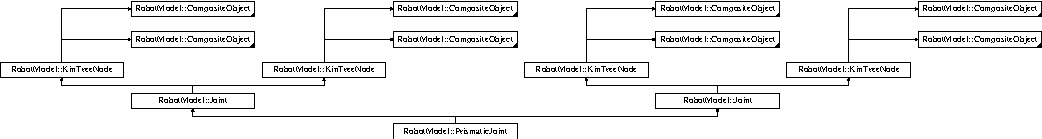
\includegraphics[height=1.8617cm]{class_robot_model_1_1_prismatic_joint}
\end{center}
\end{figure}
\subsection*{Public Member Functions}
\begin{DoxyCompactItemize}
\item 
\hyperlink{class_robot_model_1_1_prismatic_joint_a0a842b2415dafda9a87c854925fdc0b7}{PrismaticJoint} (\hyperlink{class_robot_model_1_1_robot}{Robot} $\ast$robot, \hyperlink{class_robot_model_1_1_kin_tree_node}{KinTreeNode} $\ast$parent, \hyperlink{class_robot_model_1_1_motor}{Motor} $\ast$\hyperlink{class_robot_model_1_1_joint_a8e8165df2271b16ab446028ee6bfa1c6}{motor})
\item 
\hyperlink{class_robot_model_1_1_prismatic_joint_ac519746607de0857d42c6625f4e99e60}{PrismaticJoint} (\hyperlink{class_robot_model_1_1_robot}{Robot} $\ast$robot, \hyperlink{class_robot_model_1_1_kin_tree_node}{KinTreeNode} $\ast$parent, \hyperlink{class_robot_model_1_1_motor}{Motor} $\ast$\hyperlink{class_robot_model_1_1_joint_a8e8165df2271b16ab446028ee6bfa1c6}{motor})
\end{DoxyCompactItemize}


\subsection{Constructor \& Destructor Documentation}
\hypertarget{class_robot_model_1_1_prismatic_joint_a0a842b2415dafda9a87c854925fdc0b7}{
\index{RobotModel::PrismaticJoint@{RobotModel::PrismaticJoint}!PrismaticJoint@{PrismaticJoint}}
\index{PrismaticJoint@{PrismaticJoint}!RobotModel::PrismaticJoint@{RobotModel::PrismaticJoint}}
\subsubsection[{PrismaticJoint}]{\setlength{\rightskip}{0pt plus 5cm}PrismaticJoint::PrismaticJoint ({\bf Robot} $\ast$ {\em robot}, \/  {\bf KinTreeNode} $\ast$ {\em parent}, \/  {\bf Motor} $\ast$ {\em motor})}}
\label{class_robot_model_1_1_prismatic_joint_a0a842b2415dafda9a87c854925fdc0b7}
\hypertarget{class_robot_model_1_1_prismatic_joint_ac519746607de0857d42c6625f4e99e60}{
\index{RobotModel::PrismaticJoint@{RobotModel::PrismaticJoint}!PrismaticJoint@{PrismaticJoint}}
\index{PrismaticJoint@{PrismaticJoint}!RobotModel::PrismaticJoint@{RobotModel::PrismaticJoint}}
\subsubsection[{PrismaticJoint}]{\setlength{\rightskip}{0pt plus 5cm}RobotModel::PrismaticJoint::PrismaticJoint ({\bf Robot} $\ast$ {\em robot}, \/  {\bf KinTreeNode} $\ast$ {\em parent}, \/  {\bf Motor} $\ast$ {\em motor})}}
\label{class_robot_model_1_1_prismatic_joint_ac519746607de0857d42c6625f4e99e60}


The documentation for this class was generated from the following files:\begin{DoxyCompactItemize}
\item 
/Users/kail/imClever/dev/virtualSkin/include/robotModel/\hyperlink{include_2robot_model_2joint__prismatic_8h}{joint\_\-prismatic.h}\item 
/Users/kail/imClever/dev/virtualSkin/src/robotModel/\hyperlink{src_2robot_model_2joint__prismatic_8h}{joint\_\-prismatic.h}\item 
/Users/kail/imClever/dev/virtualSkin/src/robotModel/\hyperlink{joint__prismatic_8cpp}{joint\_\-prismatic.cpp}\end{DoxyCompactItemize}

\hypertarget{class_robot_model_1_1_render_list}{
\section{RobotModel::RenderList Class Reference}
\label{class_robot_model_1_1_render_list}\index{RobotModel::RenderList@{RobotModel::RenderList}}
}


{\ttfamily \#include $<$renderList.h$>$}Inheritance diagram for RobotModel::RenderList::\begin{figure}[H]
\begin{center}
\leavevmode
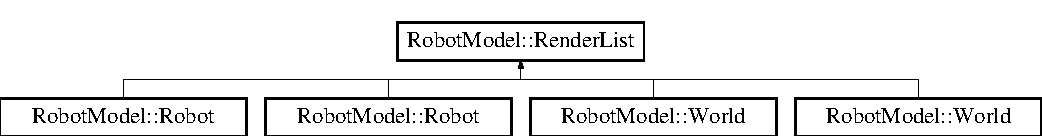
\includegraphics[height=2cm]{class_robot_model_1_1_render_list}
\end{center}
\end{figure}
\subsection*{Public Slots}
\begin{DoxyCompactItemize}
\item 
void \hyperlink{class_robot_model_1_1_render_list_a7cd62d6e6376bc02bd4244dcc174b465}{callLists} ()
\end{DoxyCompactItemize}
\subsection*{Signals}
\begin{DoxyCompactItemize}
\item 
void \hyperlink{class_robot_model_1_1_render_list_a635908222fa71402918e31eb2d725844}{appendedObject} (\hyperlink{class_robot_model_1_1_display_list}{RobotModel::DisplayList} $\ast$list)
\item 
void \hyperlink{class_robot_model_1_1_render_list_a22724d5d6878f19b639b5b6b16963ee2}{outdatedDisplayList} (int idx)
\item 
void \hyperlink{class_robot_model_1_1_render_list_a9ad71d6ea6d0d1008e0705ced20f6aea}{changedState} ()
\end{DoxyCompactItemize}
\subsection*{Public Member Functions}
\begin{DoxyCompactItemize}
\item 
\hyperlink{class_robot_model_1_1_render_list_a98651fa6cd408cce14d6d245cd95fde4}{RenderList} ()
\item 
virtual \hyperlink{class_robot_model_1_1_render_list_ae66a9f72d814771e42d7e50946053ef7}{$\sim$RenderList} ()
\item 
virtual void \hyperlink{class_robot_model_1_1_render_list_ac8646765beee22bf11582049dc3cf195}{render} ()=0
\item 
virtual void \hyperlink{class_robot_model_1_1_render_list_a78436c997913ce9ad41a9bd1da9b3d96}{notColliding} ()=0
\end{DoxyCompactItemize}


\subsection{Constructor \& Destructor Documentation}
\hypertarget{class_robot_model_1_1_render_list_a98651fa6cd408cce14d6d245cd95fde4}{
\index{RobotModel::RenderList@{RobotModel::RenderList}!RenderList@{RenderList}}
\index{RenderList@{RenderList}!RobotModel::RenderList@{RobotModel::RenderList}}
\subsubsection[{RenderList}]{\setlength{\rightskip}{0pt plus 5cm}RenderList::RenderList ()}}
\label{class_robot_model_1_1_render_list_a98651fa6cd408cce14d6d245cd95fde4}
\hypertarget{class_robot_model_1_1_render_list_ae66a9f72d814771e42d7e50946053ef7}{
\index{RobotModel::RenderList@{RobotModel::RenderList}!$\sim$RenderList@{$\sim$RenderList}}
\index{$\sim$RenderList@{$\sim$RenderList}!RobotModel::RenderList@{RobotModel::RenderList}}
\subsubsection[{$\sim$RenderList}]{\setlength{\rightskip}{0pt plus 5cm}RenderList::$\sim$RenderList ()\hspace{0.3cm}{\ttfamily  \mbox{[}virtual\mbox{]}}}}
\label{class_robot_model_1_1_render_list_ae66a9f72d814771e42d7e50946053ef7}


\subsection{Member Function Documentation}
\hypertarget{class_robot_model_1_1_render_list_a635908222fa71402918e31eb2d725844}{
\index{RobotModel::RenderList@{RobotModel::RenderList}!appendedObject@{appendedObject}}
\index{appendedObject@{appendedObject}!RobotModel::RenderList@{RobotModel::RenderList}}
\subsubsection[{appendedObject}]{\setlength{\rightskip}{0pt plus 5cm}void RobotModel::RenderList::appendedObject ({\bf RobotModel::DisplayList} $\ast$ {\em list})\hspace{0.3cm}{\ttfamily  \mbox{[}signal\mbox{]}}}}
\label{class_robot_model_1_1_render_list_a635908222fa71402918e31eb2d725844}
\hypertarget{class_robot_model_1_1_render_list_a7cd62d6e6376bc02bd4244dcc174b465}{
\index{RobotModel::RenderList@{RobotModel::RenderList}!callLists@{callLists}}
\index{callLists@{callLists}!RobotModel::RenderList@{RobotModel::RenderList}}
\subsubsection[{callLists}]{\setlength{\rightskip}{0pt plus 5cm}void RobotModel::RenderList::callLists ()\hspace{0.3cm}{\ttfamily  \mbox{[}inline, slot\mbox{]}}}}
\label{class_robot_model_1_1_render_list_a7cd62d6e6376bc02bd4244dcc174b465}
\hypertarget{class_robot_model_1_1_render_list_a9ad71d6ea6d0d1008e0705ced20f6aea}{
\index{RobotModel::RenderList@{RobotModel::RenderList}!changedState@{changedState}}
\index{changedState@{changedState}!RobotModel::RenderList@{RobotModel::RenderList}}
\subsubsection[{changedState}]{\setlength{\rightskip}{0pt plus 5cm}void RobotModel::RenderList::changedState ()\hspace{0.3cm}{\ttfamily  \mbox{[}signal\mbox{]}}}}
\label{class_robot_model_1_1_render_list_a9ad71d6ea6d0d1008e0705ced20f6aea}
\hypertarget{class_robot_model_1_1_render_list_a78436c997913ce9ad41a9bd1da9b3d96}{
\index{RobotModel::RenderList@{RobotModel::RenderList}!notColliding@{notColliding}}
\index{notColliding@{notColliding}!RobotModel::RenderList@{RobotModel::RenderList}}
\subsubsection[{notColliding}]{\setlength{\rightskip}{0pt plus 5cm}virtual void RobotModel::RenderList::notColliding ()\hspace{0.3cm}{\ttfamily  \mbox{[}pure virtual\mbox{]}}}}
\label{class_robot_model_1_1_render_list_a78436c997913ce9ad41a9bd1da9b3d96}


Implemented in \hyperlink{class_robot_model_1_1_robot_af9d5c7808f2d11ec66d905bb8606447e}{RobotModel::Robot}, and \hyperlink{class_robot_model_1_1_world_a2300046adaa75a432476dbef1934bb01}{RobotModel::World}.\hypertarget{class_robot_model_1_1_render_list_a22724d5d6878f19b639b5b6b16963ee2}{
\index{RobotModel::RenderList@{RobotModel::RenderList}!outdatedDisplayList@{outdatedDisplayList}}
\index{outdatedDisplayList@{outdatedDisplayList}!RobotModel::RenderList@{RobotModel::RenderList}}
\subsubsection[{outdatedDisplayList}]{\setlength{\rightskip}{0pt plus 5cm}void RobotModel::RenderList::outdatedDisplayList (int {\em idx})\hspace{0.3cm}{\ttfamily  \mbox{[}signal\mbox{]}}}}
\label{class_robot_model_1_1_render_list_a22724d5d6878f19b639b5b6b16963ee2}
\hypertarget{class_robot_model_1_1_render_list_ac8646765beee22bf11582049dc3cf195}{
\index{RobotModel::RenderList@{RobotModel::RenderList}!render@{render}}
\index{render@{render}!RobotModel::RenderList@{RobotModel::RenderList}}
\subsubsection[{render}]{\setlength{\rightskip}{0pt plus 5cm}virtual void RobotModel::RenderList::render ()\hspace{0.3cm}{\ttfamily  \mbox{[}pure virtual\mbox{]}}}}
\label{class_robot_model_1_1_render_list_ac8646765beee22bf11582049dc3cf195}


Implemented in \hyperlink{class_robot_model_1_1_robot_a47e480a4cad58266d12efce34f3fb563}{RobotModel::Robot}, and \hyperlink{class_robot_model_1_1_world_a150eab10c21532162bb698d72aecec16}{RobotModel::World}.

The documentation for this class was generated from the following files:\begin{DoxyCompactItemize}
\item 
/Users/kail/imClever/dev/virtualSkin/src/robotModel/\hyperlink{render_list_8h}{renderList.h}\item 
/Users/kail/imClever/dev/virtualSkin/src/robotModel/\hyperlink{render_list_8cpp}{renderList.cpp}\end{DoxyCompactItemize}

\hypertarget{class_response_observer}{
\section{ResponseObserver Class Reference}
\label{class_response_observer}\index{ResponseObserver@{ResponseObserver}}
}


{\ttfamily \#include $<$ResponseObserver.h$>$}Inheritance diagram for ResponseObserver::\begin{figure}[H]
\begin{center}
\leavevmode
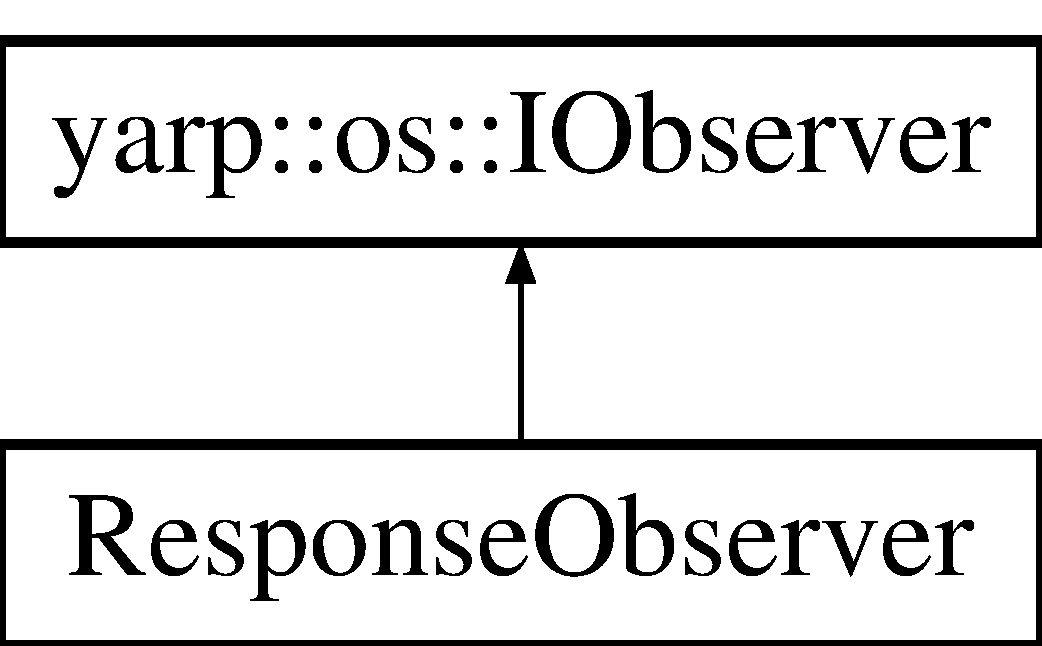
\includegraphics[height=2cm]{class_response_observer}
\end{center}
\end{figure}
\subsection*{Public Member Functions}
\begin{DoxyCompactItemize}
\item 
\hyperlink{class_response_observer_ac958ccf1a3b7667ef26449a998e5b5be}{ResponseObserver} (\hyperlink{class_robot_model_1_1_robot}{RobotModel::Robot} $\ast$r, const int b)
\item 
virtual \hyperlink{class_response_observer_aabadfb48e9895cec34fe2b54e157739b}{$\sim$ResponseObserver} ()
\item 
virtual void \hyperlink{class_response_observer_a2d847c448b31b5aa880b9282f7bf223d}{onDataObserved} (yarp::os::Bottle \&b)
\end{DoxyCompactItemize}
\subsection*{Friends}
\begin{DoxyCompactItemize}
\item 
class \hyperlink{class_response_observer_a83863f807465c9f8598a4ff381be0506}{CallObserver}
\end{DoxyCompactItemize}


\subsection{Constructor \& Destructor Documentation}
\hypertarget{class_response_observer_ac958ccf1a3b7667ef26449a998e5b5be}{
\index{ResponseObserver@{ResponseObserver}!ResponseObserver@{ResponseObserver}}
\index{ResponseObserver@{ResponseObserver}!ResponseObserver@{ResponseObserver}}
\subsubsection[{ResponseObserver}]{\setlength{\rightskip}{0pt plus 5cm}ResponseObserver::ResponseObserver ({\bf RobotModel::Robot} $\ast$ {\em r}, \/  const int {\em b})}}
\label{class_response_observer_ac958ccf1a3b7667ef26449a998e5b5be}
\hypertarget{class_response_observer_aabadfb48e9895cec34fe2b54e157739b}{
\index{ResponseObserver@{ResponseObserver}!$\sim$ResponseObserver@{$\sim$ResponseObserver}}
\index{$\sim$ResponseObserver@{$\sim$ResponseObserver}!ResponseObserver@{ResponseObserver}}
\subsubsection[{$\sim$ResponseObserver}]{\setlength{\rightskip}{0pt plus 5cm}ResponseObserver::$\sim$ResponseObserver ()\hspace{0.3cm}{\ttfamily  \mbox{[}virtual\mbox{]}}}}
\label{class_response_observer_aabadfb48e9895cec34fe2b54e157739b}


\subsection{Member Function Documentation}
\hypertarget{class_response_observer_a2d847c448b31b5aa880b9282f7bf223d}{
\index{ResponseObserver@{ResponseObserver}!onDataObserved@{onDataObserved}}
\index{onDataObserved@{onDataObserved}!ResponseObserver@{ResponseObserver}}
\subsubsection[{onDataObserved}]{\setlength{\rightskip}{0pt plus 5cm}void ResponseObserver::onDataObserved (yarp::os::Bottle \& {\em b})\hspace{0.3cm}{\ttfamily  \mbox{[}virtual\mbox{]}}}}
\label{class_response_observer_a2d847c448b31b5aa880b9282f7bf223d}
This function is called by filters to inform the implementing objects on data flowing in or out a the calling filter (RpcFilter as well as StreamFilter). 

Implements \hyperlink{classyarp_1_1os_1_1_i_observer_a4829e5a6f2ba6666b9539a4a30f20790}{yarp::os::IObserver}.

\subsection{Friends And Related Function Documentation}
\hypertarget{class_response_observer_a83863f807465c9f8598a4ff381be0506}{
\index{ResponseObserver@{ResponseObserver}!CallObserver@{CallObserver}}
\index{CallObserver@{CallObserver}!ResponseObserver@{ResponseObserver}}
\subsubsection[{CallObserver}]{\setlength{\rightskip}{0pt plus 5cm}friend class {\bf CallObserver}\hspace{0.3cm}{\ttfamily  \mbox{[}friend\mbox{]}}}}
\label{class_response_observer_a83863f807465c9f8598a4ff381be0506}


The documentation for this class was generated from the following files:\begin{DoxyCompactItemize}
\item 
/Users/kail/imClever/dev/virtualSkin/src/reflex/\hyperlink{_response_observer_8h}{ResponseObserver.h}\item 
/Users/kail/imClever/dev/virtualSkin/src/reflex/\hyperlink{_response_observer_8cpp}{ResponseObserver.cpp}\end{DoxyCompactItemize}

\hypertarget{class_robot_model_1_1_revolute_joint}{
\section{RobotModel::RevoluteJoint Class Reference}
\label{class_robot_model_1_1_revolute_joint}\index{RobotModel::RevoluteJoint@{RobotModel::RevoluteJoint}}
}


{\ttfamily \#include $<$joint\_\-revolute.h$>$}Inheritance diagram for RobotModel::RevoluteJoint::\begin{figure}[H]
\begin{center}
\leavevmode
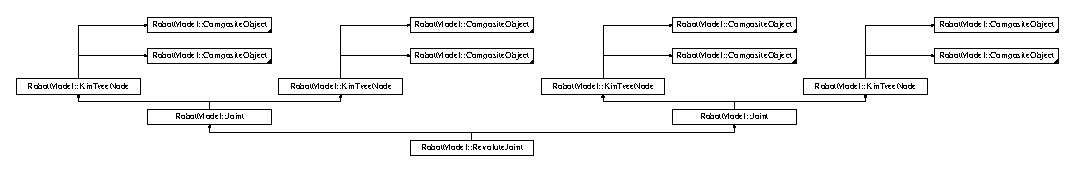
\includegraphics[height=1.8617cm]{class_robot_model_1_1_revolute_joint}
\end{center}
\end{figure}
\subsection*{Public Member Functions}
\begin{DoxyCompactItemize}
\item 
\hyperlink{class_robot_model_1_1_revolute_joint_afa148418b3aeabb6294dcb8bdc033208}{RevoluteJoint} (\hyperlink{class_robot_model_1_1_robot}{Robot} $\ast$robot, \hyperlink{class_robot_model_1_1_kin_tree_node}{KinTreeNode} $\ast$parent, \hyperlink{class_robot_model_1_1_motor}{Motor} $\ast$\hyperlink{class_robot_model_1_1_joint_a8e8165df2271b16ab446028ee6bfa1c6}{motor})
\item 
\hyperlink{class_robot_model_1_1_revolute_joint_aecc7fa3eae25c360a903ff89e196b576}{RevoluteJoint} (\hyperlink{class_robot_model_1_1_robot}{Robot} $\ast$robot, \hyperlink{class_robot_model_1_1_kin_tree_node}{KinTreeNode} $\ast$parent, \hyperlink{class_robot_model_1_1_motor}{Motor} $\ast$\hyperlink{class_robot_model_1_1_joint_a8e8165df2271b16ab446028ee6bfa1c6}{motor})
\end{DoxyCompactItemize}


\subsection{Constructor \& Destructor Documentation}
\hypertarget{class_robot_model_1_1_revolute_joint_afa148418b3aeabb6294dcb8bdc033208}{
\index{RobotModel::RevoluteJoint@{RobotModel::RevoluteJoint}!RevoluteJoint@{RevoluteJoint}}
\index{RevoluteJoint@{RevoluteJoint}!RobotModel::RevoluteJoint@{RobotModel::RevoluteJoint}}
\subsubsection[{RevoluteJoint}]{\setlength{\rightskip}{0pt plus 5cm}RevoluteJoint::RevoluteJoint ({\bf Robot} $\ast$ {\em robot}, \/  {\bf KinTreeNode} $\ast$ {\em parent}, \/  {\bf Motor} $\ast$ {\em motor})}}
\label{class_robot_model_1_1_revolute_joint_afa148418b3aeabb6294dcb8bdc033208}
\hypertarget{class_robot_model_1_1_revolute_joint_aecc7fa3eae25c360a903ff89e196b576}{
\index{RobotModel::RevoluteJoint@{RobotModel::RevoluteJoint}!RevoluteJoint@{RevoluteJoint}}
\index{RevoluteJoint@{RevoluteJoint}!RobotModel::RevoluteJoint@{RobotModel::RevoluteJoint}}
\subsubsection[{RevoluteJoint}]{\setlength{\rightskip}{0pt plus 5cm}RobotModel::RevoluteJoint::RevoluteJoint ({\bf Robot} $\ast$ {\em robot}, \/  {\bf KinTreeNode} $\ast$ {\em parent}, \/  {\bf Motor} $\ast$ {\em motor})}}
\label{class_robot_model_1_1_revolute_joint_aecc7fa3eae25c360a903ff89e196b576}


The documentation for this class was generated from the following files:\begin{DoxyCompactItemize}
\item 
/Users/kail/imClever/dev/virtualSkin/include/robotModel/\hyperlink{include_2robot_model_2joint__revolute_8h}{joint\_\-revolute.h}\item 
/Users/kail/imClever/dev/virtualSkin/src/robotModel/\hyperlink{src_2robot_model_2joint__revolute_8h}{joint\_\-revolute.h}\item 
/Users/kail/imClever/dev/virtualSkin/src/robotModel/\hyperlink{joint__revolute_8cpp}{joint\_\-revolute.cpp}\end{DoxyCompactItemize}

\hypertarget{class_robot_model_1_1_robot}{
\section{RobotModel::Robot Class Reference}
\label{class_robot_model_1_1_robot}\index{RobotModel::Robot@{RobotModel::Robot}}
}


A kinematic model of a robot.  


{\ttfamily \#include $<$robot.h$>$}Inheritance diagram for RobotModel::Robot::\begin{figure}[H]
\begin{center}
\leavevmode
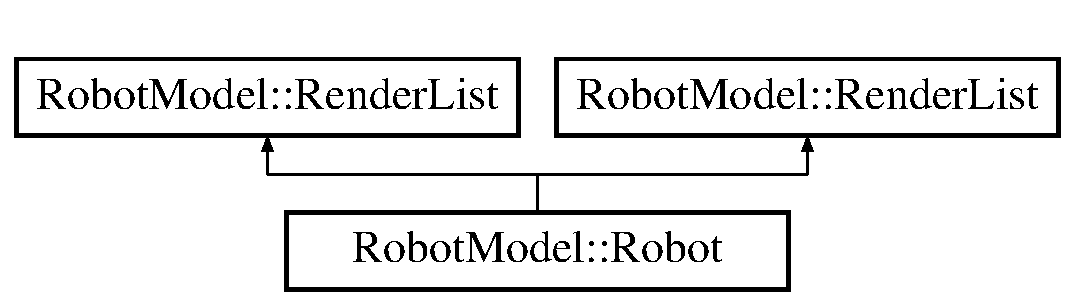
\includegraphics[height=2cm]{class_robot_model_1_1_robot}
\end{center}
\end{figure}
\subsection*{Public Member Functions}
\begin{DoxyCompactItemize}
\item 
\hyperlink{class_robot_model_1_1_robot_a4fc7c70ae20623f05e06f2ecb388b6c4}{Robot} ()
\item 
\hyperlink{class_robot_model_1_1_robot_a924320124b09c2f2ac1621aa210d5f38}{$\sim$Robot} ()
\item 
void \hyperlink{class_robot_model_1_1_robot_a0e3187d8a543ab03029138ea836ed546}{setName} (const QString \&name)
\item 
void \hyperlink{class_robot_model_1_1_robot_a44d1922d7d9ea6c7c90360c2443b1ec3}{appendBodyPart} (\hyperlink{class_robot_model_1_1_body_part}{BodyPart} $\ast$part)
\item 
void \hyperlink{class_robot_model_1_1_robot_aa4db18e00b4e4c56a37943a0b45d1c3b}{appendMotor} (\hyperlink{class_robot_model_1_1_motor}{Motor} $\ast$motor)
\item 
void \hyperlink{class_robot_model_1_1_robot_a2521948f148183c97428155be0eea923}{resizeMotorList} (int size)
\item 
void \hyperlink{class_robot_model_1_1_robot_aa6a72690fe4b0d1a2178f5478d3829bf}{appendNode} (\hyperlink{class_robot_model_1_1_kin_tree_node}{KinTreeNode} $\ast$node)
\item 
const QString \& \hyperlink{class_robot_model_1_1_robot_a07a4dcd2c34da89415576c53b42d9406}{getName} () const 
\item 
int \hyperlink{class_robot_model_1_1_robot_a16f942cf3364608585f5a352be0dc286}{getNumBodyParts} () const 
\item 
int \hyperlink{class_robot_model_1_1_robot_ad2827f8919f3cce0d39b89fb3fb33217}{nextPartIdx} () const 
\item 
int \hyperlink{class_robot_model_1_1_robot_ac9919cc40764e47d97fa591018bfbe67}{nextMotorIdx} () const 
\item 
int \hyperlink{class_robot_model_1_1_robot_a465bb3898172af37d6dec1885da0fec0}{nextLinkIdx} ()
\item 
\hyperlink{class_robot_model_1_1_body_part}{BodyPart} $\ast$ \hyperlink{class_robot_model_1_1_robot_af23f77831c87476ad0a43c624dd4b254}{getPartByName} (const QString \&partName)
\item 
\hyperlink{class_robot_model_1_1_motor}{Motor} $\ast$ \hyperlink{class_robot_model_1_1_robot_a41d959b8a9f469ee1caa5e3881a9445f}{getMotorByName} (const QString \&motorName)
\item 
const QString $\ast$ \hyperlink{class_robot_model_1_1_robot_a18b266083c6b87d05d1dc3479409e287}{getMotorName} (int partNum, int motorNum) const 
\begin{DoxyCompactList}\small\item\em Return the name of a \hyperlink{class_robot_model_1_1_motor}{Motor}. \item\end{DoxyCompactList}\item 
const QString $\ast$ \hyperlink{class_robot_model_1_1_robot_a108ec79a213fbc7655595f1716150436}{getPartName} (int partNum) const 
\begin{DoxyCompactList}\small\item\em Return the name of the \hyperlink{class_robot_model_1_1_motor}{Motor} control group. \item\end{DoxyCompactList}\item 
int \hyperlink{class_robot_model_1_1_robot_ac291608df7ce0cbe818d2da837ca008a}{getNumMotors} (int partNum) const 
\begin{DoxyCompactList}\small\item\em Return the number of motors in the group branchNum. \item\end{DoxyCompactList}\item 
virtual void \hyperlink{class_robot_model_1_1_robot_a47e480a4cad58266d12efce34f3fb563}{render} ()
\begin{DoxyCompactList}\small\item\em Return the number of \hyperlink{class_robot_model_1_1_motor}{Motor} groups. \item\end{DoxyCompactList}\item 
virtual void \hyperlink{class_robot_model_1_1_robot_af9d5c7808f2d11ec66d905bb8606447e}{notColliding} ()
\item 
void \hyperlink{class_robot_model_1_1_robot_a791f90ebca15e9a1e61e9e903f7dc594}{printLinks} ()
\begin{DoxyCompactList}\small\item\em Print the \hyperlink{class_robot_model_1_1_link}{Link} Tree. \item\end{DoxyCompactList}\item 
void \hyperlink{class_robot_model_1_1_robot_ad67fe62de4ea2b7b6da0521fc0bf0e5a}{printBodyParts} ()
\begin{DoxyCompactList}\small\item\em Print the \hyperlink{class_robot_model_1_1_motor}{Motor} control groups. \item\end{DoxyCompactList}\item 
bool \hyperlink{class_robot_model_1_1_robot_a9ca9887b212f3233d101d95854cf2c79}{configure} (const QString \&fileName)
\begin{DoxyCompactList}\small\item\em Initialize the \hyperlink{class_robot_model_1_1_robot}{Robot}. \item\end{DoxyCompactList}\item 
void \hyperlink{class_robot_model_1_1_robot_a72ff62b72e0e9d34d3ca0c241dec50d3}{setEncoderPosition} (qreal pos=0)
\begin{DoxyCompactList}\small\item\em Set the position of every joint on the robot. \item\end{DoxyCompactList}\item 
bool \hyperlink{class_robot_model_1_1_robot_ad68d3bd2d8edbca49704f8a5b01055a1}{setEncoderPosition} (int partNum, const QVector$<$ qreal $>$ \&pos)
\begin{DoxyCompactList}\small\item\em Set the positions of all motors in the group branchNum. \item\end{DoxyCompactList}\item 
bool \hyperlink{class_robot_model_1_1_robot_a08017bce09f838437534aec53d615ff6}{setEncoderPosition} (int partNum, int motorNum, qreal pos)
\begin{DoxyCompactList}\small\item\em Set the position of a single \hyperlink{class_robot_model_1_1_motor}{Motor}. \item\end{DoxyCompactList}\item 
void \hyperlink{class_robot_model_1_1_robot_a2fd7c2a0cd53593361f38f52de41d73c}{home} ()
\begin{DoxyCompactList}\small\item\em Update the pose of the \hyperlink{class_robot_model_1_1_robot}{Robot}. \item\end{DoxyCompactList}\item 
void \hyperlink{class_robot_model_1_1_robot_a7338994f0ab4baa6e5d08751272b63ca}{updatePose} ()
\item 
void \hyperlink{class_robot_model_1_1_robot_a4c006ead68b20137a28276920103667c}{emitAppended} (\hyperlink{class_robot_model_1_1_display_list}{DisplayList} $\ast$list)
\item 
\hyperlink{class_robot_model_1_1_robot_a22e9262b6ee5252f9a5171b004879b4b}{Robot} ()
\item 
\hyperlink{class_robot_model_1_1_robot_add0b7a3958eb4afd56983a56cc31dbfc}{$\sim$Robot} ()
\item 
void \hyperlink{class_robot_model_1_1_robot_a0e3187d8a543ab03029138ea836ed546}{setName} (const QString \&name)
\item 
void \hyperlink{class_robot_model_1_1_robot_a44d1922d7d9ea6c7c90360c2443b1ec3}{appendBodyPart} (\hyperlink{class_robot_model_1_1_body_part}{BodyPart} $\ast$part)
\item 
void \hyperlink{class_robot_model_1_1_robot_aa4db18e00b4e4c56a37943a0b45d1c3b}{appendMotor} (\hyperlink{class_robot_model_1_1_motor}{Motor} $\ast$motor)
\item 
void \hyperlink{class_robot_model_1_1_robot_a2521948f148183c97428155be0eea923}{resizeMotorList} (int size)
\item 
void \hyperlink{class_robot_model_1_1_robot_aa6a72690fe4b0d1a2178f5478d3829bf}{appendNode} (\hyperlink{class_robot_model_1_1_kin_tree_node}{KinTreeNode} $\ast$node)
\item 
const QString \& \hyperlink{class_robot_model_1_1_robot_a07a4dcd2c34da89415576c53b42d9406}{getName} () const 
\item 
int \hyperlink{class_robot_model_1_1_robot_a16f942cf3364608585f5a352be0dc286}{getNumBodyParts} () const 
\item 
int \hyperlink{class_robot_model_1_1_robot_ad2827f8919f3cce0d39b89fb3fb33217}{nextPartIdx} () const 
\item 
int \hyperlink{class_robot_model_1_1_robot_ac9919cc40764e47d97fa591018bfbe67}{nextMotorIdx} () const 
\item 
int \hyperlink{class_robot_model_1_1_robot_a465bb3898172af37d6dec1885da0fec0}{nextLinkIdx} ()
\item 
\hyperlink{class_robot_model_1_1_body_part}{BodyPart} $\ast$ \hyperlink{class_robot_model_1_1_robot_a5a24673b9e7b3a95f68cf543b6c2f7a0}{getPartByName} (const QString \&partName)
\item 
\hyperlink{class_robot_model_1_1_motor}{Motor} $\ast$ \hyperlink{class_robot_model_1_1_robot_a999c5f6c15891436fdfb97517d600a7a}{getMotorByName} (const QString \&motorName)
\item 
const QString $\ast$ \hyperlink{class_robot_model_1_1_robot_a13f6c53297cdc08f2ccf8e2c41a6efd3}{getMotorName} (int partNum, int motorNum) const 
\begin{DoxyCompactList}\small\item\em Return the name of a \hyperlink{class_robot_model_1_1_motor}{Motor}. \item\end{DoxyCompactList}\item 
const QString $\ast$ \hyperlink{class_robot_model_1_1_robot_a3fb8fb4e1d19bdf1c4c9278d2e9bcd31}{getPartName} (int partNum) const 
\begin{DoxyCompactList}\small\item\em Return the name of the \hyperlink{class_robot_model_1_1_motor}{Motor} control group. \item\end{DoxyCompactList}\item 
int \hyperlink{class_robot_model_1_1_robot_aae3de10ec98969b5def3adc436483362}{getNumMotors} (int partNum) const 
\begin{DoxyCompactList}\small\item\em Return the number of motors in the group branchNum. \item\end{DoxyCompactList}\item 
virtual void \hyperlink{class_robot_model_1_1_robot_a3be7d3c8d21aeb68633d9e176a3fbf08}{render} ()
\begin{DoxyCompactList}\small\item\em Return the number of \hyperlink{class_robot_model_1_1_motor}{Motor} groups. \item\end{DoxyCompactList}\item 
virtual void \hyperlink{class_robot_model_1_1_robot_a355a98d015e6aad905e4d2e5cf42c442}{notColliding} ()
\item 
void \hyperlink{class_robot_model_1_1_robot_a064e5fce550bb3427fb36c2f43e34000}{printLinks} ()
\begin{DoxyCompactList}\small\item\em Print the \hyperlink{class_robot_model_1_1_link}{Link} Tree. \item\end{DoxyCompactList}\item 
void \hyperlink{class_robot_model_1_1_robot_abb43fb469172e7ff9ce37a7211a81175}{printBodyParts} ()
\begin{DoxyCompactList}\small\item\em Print the \hyperlink{class_robot_model_1_1_motor}{Motor} control groups. \item\end{DoxyCompactList}\item 
bool \hyperlink{class_robot_model_1_1_robot_af54a14845b7e3ee6c4103790df71568e}{configure} (const QString \&fileName)
\begin{DoxyCompactList}\small\item\em Initialize the \hyperlink{class_robot_model_1_1_robot}{Robot}. \item\end{DoxyCompactList}\item 
void \hyperlink{class_robot_model_1_1_robot_a99dfb27d656fbec65adc1c3881d63f6f}{setEncoderPosition} (qreal pos=0)
\begin{DoxyCompactList}\small\item\em Set the position of every joint on the robot. \item\end{DoxyCompactList}\item 
bool \hyperlink{class_robot_model_1_1_robot_a0d1c835b7a107a1ff6fe36bc9cf0622e}{setEncoderPosition} (int partNum, const QVector$<$ qreal $>$ \&pos)
\begin{DoxyCompactList}\small\item\em Set the positions of all motors in the group branchNum. \item\end{DoxyCompactList}\item 
bool \hyperlink{class_robot_model_1_1_robot_a8e66688b7abcf8cadd86c463c6c97458}{setEncoderPosition} (int partNum, int motorNum, qreal pos)
\begin{DoxyCompactList}\small\item\em Set the position of a single \hyperlink{class_robot_model_1_1_motor}{Motor}. \item\end{DoxyCompactList}\item 
void \hyperlink{class_robot_model_1_1_robot_a6238d22c6617eb9b56dba349851d6119}{home} ()
\begin{DoxyCompactList}\small\item\em Update the pose of the \hyperlink{class_robot_model_1_1_robot}{Robot}. \item\end{DoxyCompactList}\item 
void \hyperlink{class_robot_model_1_1_robot_a7dc3d1bbf0e7f297503a7ed8c89dd63b}{updatePose} ()
\item 
void \hyperlink{class_robot_model_1_1_robot_a4c006ead68b20137a28276920103667c}{emitAppended} (\hyperlink{class_robot_model_1_1_display_list}{DisplayList} $\ast$list)
\end{DoxyCompactItemize}
\subsection*{Friends}
\begin{DoxyCompactItemize}
\item 
class \hyperlink{class_robot_model_1_1_robot_a3dae6d594db374d61cfe7a7701326056}{KinTreeNode}
\end{DoxyCompactItemize}


\subsection{Detailed Description}
A kinematic model of a robot. The model consists of a tree of \hyperlink{class_robot_model_1_1_link}{Link} objects, some of which are \hyperlink{class_robot_model_1_1_joint}{Joint} objects, as well as a list of \hyperlink{class_robot_model_1_1_motor}{Motor} objects and a list of Branch objects. Motors are bound to joints and control the joints' position according to a linear mapping. Brnaches are groups of motors, accessable via a vector (see RobotInterface::setPos(int,QVector$<$qreal$>$)). The \hyperlink{class_robot_model_1_1_robot}{Robot} class is primarily a container, and the tree as well as the lists are populated by the constructors of Branch, \hyperlink{class_robot_model_1_1_motor}{Motor} and \hyperlink{class_robot_model_1_1_link}{Link}, which are friend functions of this class. 

\subsection{Constructor \& Destructor Documentation}
\hypertarget{class_robot_model_1_1_robot_a4fc7c70ae20623f05e06f2ecb388b6c4}{
\index{RobotModel::Robot@{RobotModel::Robot}!Robot@{Robot}}
\index{Robot@{Robot}!RobotModel::Robot@{RobotModel::Robot}}
\subsubsection[{Robot}]{\setlength{\rightskip}{0pt plus 5cm}Robot::Robot ()}}
\label{class_robot_model_1_1_robot_a4fc7c70ae20623f05e06f2ecb388b6c4}
\hypertarget{class_robot_model_1_1_robot_a924320124b09c2f2ac1621aa210d5f38}{
\index{RobotModel::Robot@{RobotModel::Robot}!$\sim$Robot@{$\sim$Robot}}
\index{$\sim$Robot@{$\sim$Robot}!RobotModel::Robot@{RobotModel::Robot}}
\subsubsection[{$\sim$Robot}]{\setlength{\rightskip}{0pt plus 5cm}Robot::$\sim$Robot ()}}
\label{class_robot_model_1_1_robot_a924320124b09c2f2ac1621aa210d5f38}
\hypertarget{class_robot_model_1_1_robot_a22e9262b6ee5252f9a5171b004879b4b}{
\index{RobotModel::Robot@{RobotModel::Robot}!Robot@{Robot}}
\index{Robot@{Robot}!RobotModel::Robot@{RobotModel::Robot}}
\subsubsection[{Robot}]{\setlength{\rightskip}{0pt plus 5cm}RobotModel::Robot::Robot ()}}
\label{class_robot_model_1_1_robot_a22e9262b6ee5252f9a5171b004879b4b}
\hypertarget{class_robot_model_1_1_robot_add0b7a3958eb4afd56983a56cc31dbfc}{
\index{RobotModel::Robot@{RobotModel::Robot}!$\sim$Robot@{$\sim$Robot}}
\index{$\sim$Robot@{$\sim$Robot}!RobotModel::Robot@{RobotModel::Robot}}
\subsubsection[{$\sim$Robot}]{\setlength{\rightskip}{0pt plus 5cm}RobotModel::Robot::$\sim$Robot ()}}
\label{class_robot_model_1_1_robot_add0b7a3958eb4afd56983a56cc31dbfc}


\subsection{Member Function Documentation}
\hypertarget{class_robot_model_1_1_robot_a44d1922d7d9ea6c7c90360c2443b1ec3}{
\index{RobotModel::Robot@{RobotModel::Robot}!appendBodyPart@{appendBodyPart}}
\index{appendBodyPart@{appendBodyPart}!RobotModel::Robot@{RobotModel::Robot}}
\subsubsection[{appendBodyPart}]{\setlength{\rightskip}{0pt plus 5cm}void RobotModel::Robot::appendBodyPart ({\bf BodyPart} $\ast$ {\em part})\hspace{0.3cm}{\ttfamily  \mbox{[}inline\mbox{]}}}}
\label{class_robot_model_1_1_robot_a44d1922d7d9ea6c7c90360c2443b1ec3}
\hypertarget{class_robot_model_1_1_robot_a44d1922d7d9ea6c7c90360c2443b1ec3}{
\index{RobotModel::Robot@{RobotModel::Robot}!appendBodyPart@{appendBodyPart}}
\index{appendBodyPart@{appendBodyPart}!RobotModel::Robot@{RobotModel::Robot}}
\subsubsection[{appendBodyPart}]{\setlength{\rightskip}{0pt plus 5cm}void RobotModel::Robot::appendBodyPart ({\bf BodyPart} $\ast$ {\em part})\hspace{0.3cm}{\ttfamily  \mbox{[}inline\mbox{]}}}}
\label{class_robot_model_1_1_robot_a44d1922d7d9ea6c7c90360c2443b1ec3}
\hypertarget{class_robot_model_1_1_robot_aa4db18e00b4e4c56a37943a0b45d1c3b}{
\index{RobotModel::Robot@{RobotModel::Robot}!appendMotor@{appendMotor}}
\index{appendMotor@{appendMotor}!RobotModel::Robot@{RobotModel::Robot}}
\subsubsection[{appendMotor}]{\setlength{\rightskip}{0pt plus 5cm}void RobotModel::Robot::appendMotor ({\bf Motor} $\ast$ {\em motor})\hspace{0.3cm}{\ttfamily  \mbox{[}inline\mbox{]}}}}
\label{class_robot_model_1_1_robot_aa4db18e00b4e4c56a37943a0b45d1c3b}
\hypertarget{class_robot_model_1_1_robot_aa4db18e00b4e4c56a37943a0b45d1c3b}{
\index{RobotModel::Robot@{RobotModel::Robot}!appendMotor@{appendMotor}}
\index{appendMotor@{appendMotor}!RobotModel::Robot@{RobotModel::Robot}}
\subsubsection[{appendMotor}]{\setlength{\rightskip}{0pt plus 5cm}void RobotModel::Robot::appendMotor ({\bf Motor} $\ast$ {\em motor})\hspace{0.3cm}{\ttfamily  \mbox{[}inline\mbox{]}}}}
\label{class_robot_model_1_1_robot_aa4db18e00b4e4c56a37943a0b45d1c3b}
\hypertarget{class_robot_model_1_1_robot_aa6a72690fe4b0d1a2178f5478d3829bf}{
\index{RobotModel::Robot@{RobotModel::Robot}!appendNode@{appendNode}}
\index{appendNode@{appendNode}!RobotModel::Robot@{RobotModel::Robot}}
\subsubsection[{appendNode}]{\setlength{\rightskip}{0pt plus 5cm}void RobotModel::Robot::appendNode ({\bf KinTreeNode} $\ast$ {\em node})\hspace{0.3cm}{\ttfamily  \mbox{[}inline\mbox{]}}}}
\label{class_robot_model_1_1_robot_aa6a72690fe4b0d1a2178f5478d3829bf}
\hypertarget{class_robot_model_1_1_robot_aa6a72690fe4b0d1a2178f5478d3829bf}{
\index{RobotModel::Robot@{RobotModel::Robot}!appendNode@{appendNode}}
\index{appendNode@{appendNode}!RobotModel::Robot@{RobotModel::Robot}}
\subsubsection[{appendNode}]{\setlength{\rightskip}{0pt plus 5cm}void RobotModel::Robot::appendNode ({\bf KinTreeNode} $\ast$ {\em node})\hspace{0.3cm}{\ttfamily  \mbox{[}inline\mbox{]}}}}
\label{class_robot_model_1_1_robot_aa6a72690fe4b0d1a2178f5478d3829bf}
\hypertarget{class_robot_model_1_1_robot_af54a14845b7e3ee6c4103790df71568e}{
\index{RobotModel::Robot@{RobotModel::Robot}!configure@{configure}}
\index{configure@{configure}!RobotModel::Robot@{RobotModel::Robot}}
\subsubsection[{configure}]{\setlength{\rightskip}{0pt plus 5cm}bool RobotModel::Robot::configure (const QString \& {\em fileName})}}
\label{class_robot_model_1_1_robot_af54a14845b7e3ee6c4103790df71568e}


Initialize the \hyperlink{class_robot_model_1_1_robot}{Robot}. Parse the robot configuration XML file and call constructors of \hyperlink{class_robot_model_1_1_link}{Link}, \hyperlink{class_robot_model_1_1_joint}{Joint}, \hyperlink{class_robot_model_1_1_motor}{Motor}, and Branch, to build up the \hyperlink{class_robot_model_1_1_robot}{Robot}. ZPRobotHandler, which inherits QXmlDefaultHandler, calls the constructors. \hypertarget{class_robot_model_1_1_robot_a9ca9887b212f3233d101d95854cf2c79}{
\index{RobotModel::Robot@{RobotModel::Robot}!configure@{configure}}
\index{configure@{configure}!RobotModel::Robot@{RobotModel::Robot}}
\subsubsection[{configure}]{\setlength{\rightskip}{0pt plus 5cm}bool Robot::configure (const QString \& {\em fileName})}}
\label{class_robot_model_1_1_robot_a9ca9887b212f3233d101d95854cf2c79}


Initialize the \hyperlink{class_robot_model_1_1_robot}{Robot}. Parse the robot configuration XML file and call constructors of \hyperlink{class_robot_model_1_1_link}{Link}, \hyperlink{class_robot_model_1_1_joint}{Joint}, \hyperlink{class_robot_model_1_1_motor}{Motor}, and Branch, to build up the \hyperlink{class_robot_model_1_1_robot}{Robot}. ZPRobotHandler, which inherits QXmlDefaultHandler, calls the constructors. \hypertarget{class_robot_model_1_1_robot_a4c006ead68b20137a28276920103667c}{
\index{RobotModel::Robot@{RobotModel::Robot}!emitAppended@{emitAppended}}
\index{emitAppended@{emitAppended}!RobotModel::Robot@{RobotModel::Robot}}
\subsubsection[{emitAppended}]{\setlength{\rightskip}{0pt plus 5cm}void RobotModel::Robot::emitAppended ({\bf DisplayList} $\ast$ {\em list})\hspace{0.3cm}{\ttfamily  \mbox{[}inline\mbox{]}}}}
\label{class_robot_model_1_1_robot_a4c006ead68b20137a28276920103667c}
\hypertarget{class_robot_model_1_1_robot_a4c006ead68b20137a28276920103667c}{
\index{RobotModel::Robot@{RobotModel::Robot}!emitAppended@{emitAppended}}
\index{emitAppended@{emitAppended}!RobotModel::Robot@{RobotModel::Robot}}
\subsubsection[{emitAppended}]{\setlength{\rightskip}{0pt plus 5cm}void RobotModel::Robot::emitAppended ({\bf DisplayList} $\ast$ {\em list})\hspace{0.3cm}{\ttfamily  \mbox{[}inline\mbox{]}}}}
\label{class_robot_model_1_1_robot_a4c006ead68b20137a28276920103667c}
\hypertarget{class_robot_model_1_1_robot_a999c5f6c15891436fdfb97517d600a7a}{
\index{RobotModel::Robot@{RobotModel::Robot}!getMotorByName@{getMotorByName}}
\index{getMotorByName@{getMotorByName}!RobotModel::Robot@{RobotModel::Robot}}
\subsubsection[{getMotorByName}]{\setlength{\rightskip}{0pt plus 5cm}{\bf Motor}$\ast$ RobotModel::Robot::getMotorByName (const QString \& {\em motorName})}}
\label{class_robot_model_1_1_robot_a999c5f6c15891436fdfb97517d600a7a}
\hypertarget{class_robot_model_1_1_robot_a41d959b8a9f469ee1caa5e3881a9445f}{
\index{RobotModel::Robot@{RobotModel::Robot}!getMotorByName@{getMotorByName}}
\index{getMotorByName@{getMotorByName}!RobotModel::Robot@{RobotModel::Robot}}
\subsubsection[{getMotorByName}]{\setlength{\rightskip}{0pt plus 5cm}{\bf Motor} $\ast$ Robot::getMotorByName (const QString \& {\em motorName})}}
\label{class_robot_model_1_1_robot_a41d959b8a9f469ee1caa5e3881a9445f}
\hypertarget{class_robot_model_1_1_robot_a13f6c53297cdc08f2ccf8e2c41a6efd3}{
\index{RobotModel::Robot@{RobotModel::Robot}!getMotorName@{getMotorName}}
\index{getMotorName@{getMotorName}!RobotModel::Robot@{RobotModel::Robot}}
\subsubsection[{getMotorName}]{\setlength{\rightskip}{0pt plus 5cm}const QString$\ast$ RobotModel::Robot::getMotorName (int {\em partNum}, \/  int {\em motorNum}) const}}
\label{class_robot_model_1_1_robot_a13f6c53297cdc08f2ccf8e2c41a6efd3}


Return the name of a \hyperlink{class_robot_model_1_1_motor}{Motor}. \hypertarget{class_robot_model_1_1_robot_a18b266083c6b87d05d1dc3479409e287}{
\index{RobotModel::Robot@{RobotModel::Robot}!getMotorName@{getMotorName}}
\index{getMotorName@{getMotorName}!RobotModel::Robot@{RobotModel::Robot}}
\subsubsection[{getMotorName}]{\setlength{\rightskip}{0pt plus 5cm}const QString $\ast$ Robot::getMotorName (int {\em partNum}, \/  int {\em motorNum}) const}}
\label{class_robot_model_1_1_robot_a18b266083c6b87d05d1dc3479409e287}


Return the name of a \hyperlink{class_robot_model_1_1_motor}{Motor}. \hypertarget{class_robot_model_1_1_robot_a07a4dcd2c34da89415576c53b42d9406}{
\index{RobotModel::Robot@{RobotModel::Robot}!getName@{getName}}
\index{getName@{getName}!RobotModel::Robot@{RobotModel::Robot}}
\subsubsection[{getName}]{\setlength{\rightskip}{0pt plus 5cm}const QString\& RobotModel::Robot::getName () const\hspace{0.3cm}{\ttfamily  \mbox{[}inline\mbox{]}}}}
\label{class_robot_model_1_1_robot_a07a4dcd2c34da89415576c53b42d9406}
\hypertarget{class_robot_model_1_1_robot_a07a4dcd2c34da89415576c53b42d9406}{
\index{RobotModel::Robot@{RobotModel::Robot}!getName@{getName}}
\index{getName@{getName}!RobotModel::Robot@{RobotModel::Robot}}
\subsubsection[{getName}]{\setlength{\rightskip}{0pt plus 5cm}const QString\& RobotModel::Robot::getName () const\hspace{0.3cm}{\ttfamily  \mbox{[}inline\mbox{]}}}}
\label{class_robot_model_1_1_robot_a07a4dcd2c34da89415576c53b42d9406}
\hypertarget{class_robot_model_1_1_robot_a16f942cf3364608585f5a352be0dc286}{
\index{RobotModel::Robot@{RobotModel::Robot}!getNumBodyParts@{getNumBodyParts}}
\index{getNumBodyParts@{getNumBodyParts}!RobotModel::Robot@{RobotModel::Robot}}
\subsubsection[{getNumBodyParts}]{\setlength{\rightskip}{0pt plus 5cm}int RobotModel::Robot::getNumBodyParts () const\hspace{0.3cm}{\ttfamily  \mbox{[}inline\mbox{]}}}}
\label{class_robot_model_1_1_robot_a16f942cf3364608585f5a352be0dc286}
\hypertarget{class_robot_model_1_1_robot_a16f942cf3364608585f5a352be0dc286}{
\index{RobotModel::Robot@{RobotModel::Robot}!getNumBodyParts@{getNumBodyParts}}
\index{getNumBodyParts@{getNumBodyParts}!RobotModel::Robot@{RobotModel::Robot}}
\subsubsection[{getNumBodyParts}]{\setlength{\rightskip}{0pt plus 5cm}int RobotModel::Robot::getNumBodyParts () const\hspace{0.3cm}{\ttfamily  \mbox{[}inline\mbox{]}}}}
\label{class_robot_model_1_1_robot_a16f942cf3364608585f5a352be0dc286}
\hypertarget{class_robot_model_1_1_robot_aae3de10ec98969b5def3adc436483362}{
\index{RobotModel::Robot@{RobotModel::Robot}!getNumMotors@{getNumMotors}}
\index{getNumMotors@{getNumMotors}!RobotModel::Robot@{RobotModel::Robot}}
\subsubsection[{getNumMotors}]{\setlength{\rightskip}{0pt plus 5cm}int RobotModel::Robot::getNumMotors (int {\em partNum}) const}}
\label{class_robot_model_1_1_robot_aae3de10ec98969b5def3adc436483362}


Return the number of motors in the group branchNum. Returns 0 if branchNum is out of range. \hypertarget{class_robot_model_1_1_robot_ac291608df7ce0cbe818d2da837ca008a}{
\index{RobotModel::Robot@{RobotModel::Robot}!getNumMotors@{getNumMotors}}
\index{getNumMotors@{getNumMotors}!RobotModel::Robot@{RobotModel::Robot}}
\subsubsection[{getNumMotors}]{\setlength{\rightskip}{0pt plus 5cm}int Robot::getNumMotors (int {\em partNum}) const}}
\label{class_robot_model_1_1_robot_ac291608df7ce0cbe818d2da837ca008a}


Return the number of motors in the group branchNum. Returns 0 if branchNum is out of range. \hypertarget{class_robot_model_1_1_robot_a5a24673b9e7b3a95f68cf543b6c2f7a0}{
\index{RobotModel::Robot@{RobotModel::Robot}!getPartByName@{getPartByName}}
\index{getPartByName@{getPartByName}!RobotModel::Robot@{RobotModel::Robot}}
\subsubsection[{getPartByName}]{\setlength{\rightskip}{0pt plus 5cm}{\bf BodyPart}$\ast$ RobotModel::Robot::getPartByName (const QString \& {\em partName})}}
\label{class_robot_model_1_1_robot_a5a24673b9e7b3a95f68cf543b6c2f7a0}
\hypertarget{class_robot_model_1_1_robot_af23f77831c87476ad0a43c624dd4b254}{
\index{RobotModel::Robot@{RobotModel::Robot}!getPartByName@{getPartByName}}
\index{getPartByName@{getPartByName}!RobotModel::Robot@{RobotModel::Robot}}
\subsubsection[{getPartByName}]{\setlength{\rightskip}{0pt plus 5cm}{\bf BodyPart} $\ast$ Robot::getPartByName (const QString \& {\em partName})}}
\label{class_robot_model_1_1_robot_af23f77831c87476ad0a43c624dd4b254}
\hypertarget{class_robot_model_1_1_robot_a3fb8fb4e1d19bdf1c4c9278d2e9bcd31}{
\index{RobotModel::Robot@{RobotModel::Robot}!getPartName@{getPartName}}
\index{getPartName@{getPartName}!RobotModel::Robot@{RobotModel::Robot}}
\subsubsection[{getPartName}]{\setlength{\rightskip}{0pt plus 5cm}const QString$\ast$ RobotModel::Robot::getPartName (int {\em partNum}) const}}
\label{class_robot_model_1_1_robot_a3fb8fb4e1d19bdf1c4c9278d2e9bcd31}


Return the name of the \hyperlink{class_robot_model_1_1_motor}{Motor} control group. If connecting to YARP, this is the name of the target control group. For the iCub, 'torso', 'arm', 'head', ect. \hypertarget{class_robot_model_1_1_robot_a108ec79a213fbc7655595f1716150436}{
\index{RobotModel::Robot@{RobotModel::Robot}!getPartName@{getPartName}}
\index{getPartName@{getPartName}!RobotModel::Robot@{RobotModel::Robot}}
\subsubsection[{getPartName}]{\setlength{\rightskip}{0pt plus 5cm}const QString $\ast$ Robot::getPartName (int {\em partNum}) const}}
\label{class_robot_model_1_1_robot_a108ec79a213fbc7655595f1716150436}


Return the name of the \hyperlink{class_robot_model_1_1_motor}{Motor} control group. If connecting to YARP, this is the name of the target control group. For the iCub, 'torso', 'arm', 'head', ect. \hypertarget{class_robot_model_1_1_robot_a6238d22c6617eb9b56dba349851d6119}{
\index{RobotModel::Robot@{RobotModel::Robot}!home@{home}}
\index{home@{home}!RobotModel::Robot@{RobotModel::Robot}}
\subsubsection[{home}]{\setlength{\rightskip}{0pt plus 5cm}void RobotModel::Robot::home ()}}
\label{class_robot_model_1_1_robot_a6238d22c6617eb9b56dba349851d6119}


Update the pose of the \hyperlink{class_robot_model_1_1_robot}{Robot}. This recursive function carries out the matrix multiplication of forward kinematics. As the position and orientation of each link in the tree is calculated, the \hyperlink{class_robot_model_1_1_link}{Link} sends a signal via the \hyperlink{class_robot_model_1_1_robot}{Robot}, Robot::NewJoint(int). \hypertarget{class_robot_model_1_1_robot_a2fd7c2a0cd53593361f38f52de41d73c}{
\index{RobotModel::Robot@{RobotModel::Robot}!home@{home}}
\index{home@{home}!RobotModel::Robot@{RobotModel::Robot}}
\subsubsection[{home}]{\setlength{\rightskip}{0pt plus 5cm}void Robot::home ()}}
\label{class_robot_model_1_1_robot_a2fd7c2a0cd53593361f38f52de41d73c}


Update the pose of the \hyperlink{class_robot_model_1_1_robot}{Robot}. This recursive function carries out the matrix multiplication of forward kinematics. As the position and orientation of each link in the tree is calculated, the \hyperlink{class_robot_model_1_1_link}{Link} sends a signal via the \hyperlink{class_robot_model_1_1_robot}{Robot}, Robot::NewJoint(int). \hypertarget{class_robot_model_1_1_robot_a465bb3898172af37d6dec1885da0fec0}{
\index{RobotModel::Robot@{RobotModel::Robot}!nextLinkIdx@{nextLinkIdx}}
\index{nextLinkIdx@{nextLinkIdx}!RobotModel::Robot@{RobotModel::Robot}}
\subsubsection[{nextLinkIdx}]{\setlength{\rightskip}{0pt plus 5cm}int RobotModel::Robot::nextLinkIdx ()\hspace{0.3cm}{\ttfamily  \mbox{[}inline\mbox{]}}}}
\label{class_robot_model_1_1_robot_a465bb3898172af37d6dec1885da0fec0}
\hypertarget{class_robot_model_1_1_robot_a465bb3898172af37d6dec1885da0fec0}{
\index{RobotModel::Robot@{RobotModel::Robot}!nextLinkIdx@{nextLinkIdx}}
\index{nextLinkIdx@{nextLinkIdx}!RobotModel::Robot@{RobotModel::Robot}}
\subsubsection[{nextLinkIdx}]{\setlength{\rightskip}{0pt plus 5cm}int RobotModel::Robot::nextLinkIdx ()\hspace{0.3cm}{\ttfamily  \mbox{[}inline\mbox{]}}}}
\label{class_robot_model_1_1_robot_a465bb3898172af37d6dec1885da0fec0}
\hypertarget{class_robot_model_1_1_robot_ac9919cc40764e47d97fa591018bfbe67}{
\index{RobotModel::Robot@{RobotModel::Robot}!nextMotorIdx@{nextMotorIdx}}
\index{nextMotorIdx@{nextMotorIdx}!RobotModel::Robot@{RobotModel::Robot}}
\subsubsection[{nextMotorIdx}]{\setlength{\rightskip}{0pt plus 5cm}int RobotModel::Robot::nextMotorIdx () const\hspace{0.3cm}{\ttfamily  \mbox{[}inline\mbox{]}}}}
\label{class_robot_model_1_1_robot_ac9919cc40764e47d97fa591018bfbe67}
\hypertarget{class_robot_model_1_1_robot_ac9919cc40764e47d97fa591018bfbe67}{
\index{RobotModel::Robot@{RobotModel::Robot}!nextMotorIdx@{nextMotorIdx}}
\index{nextMotorIdx@{nextMotorIdx}!RobotModel::Robot@{RobotModel::Robot}}
\subsubsection[{nextMotorIdx}]{\setlength{\rightskip}{0pt plus 5cm}int RobotModel::Robot::nextMotorIdx () const\hspace{0.3cm}{\ttfamily  \mbox{[}inline\mbox{]}}}}
\label{class_robot_model_1_1_robot_ac9919cc40764e47d97fa591018bfbe67}
\hypertarget{class_robot_model_1_1_robot_ad2827f8919f3cce0d39b89fb3fb33217}{
\index{RobotModel::Robot@{RobotModel::Robot}!nextPartIdx@{nextPartIdx}}
\index{nextPartIdx@{nextPartIdx}!RobotModel::Robot@{RobotModel::Robot}}
\subsubsection[{nextPartIdx}]{\setlength{\rightskip}{0pt plus 5cm}int RobotModel::Robot::nextPartIdx () const\hspace{0.3cm}{\ttfamily  \mbox{[}inline\mbox{]}}}}
\label{class_robot_model_1_1_robot_ad2827f8919f3cce0d39b89fb3fb33217}
\hypertarget{class_robot_model_1_1_robot_ad2827f8919f3cce0d39b89fb3fb33217}{
\index{RobotModel::Robot@{RobotModel::Robot}!nextPartIdx@{nextPartIdx}}
\index{nextPartIdx@{nextPartIdx}!RobotModel::Robot@{RobotModel::Robot}}
\subsubsection[{nextPartIdx}]{\setlength{\rightskip}{0pt plus 5cm}int RobotModel::Robot::nextPartIdx () const\hspace{0.3cm}{\ttfamily  \mbox{[}inline\mbox{]}}}}
\label{class_robot_model_1_1_robot_ad2827f8919f3cce0d39b89fb3fb33217}
\hypertarget{class_robot_model_1_1_robot_a355a98d015e6aad905e4d2e5cf42c442}{
\index{RobotModel::Robot@{RobotModel::Robot}!notColliding@{notColliding}}
\index{notColliding@{notColliding}!RobotModel::Robot@{RobotModel::Robot}}
\subsubsection[{notColliding}]{\setlength{\rightskip}{0pt plus 5cm}virtual void RobotModel::Robot::notColliding ()\hspace{0.3cm}{\ttfamily  \mbox{[}virtual\mbox{]}}}}
\label{class_robot_model_1_1_robot_a355a98d015e6aad905e4d2e5cf42c442}


Implements \hyperlink{class_robot_model_1_1_render_list_a78436c997913ce9ad41a9bd1da9b3d96}{RobotModel::RenderList}.\hypertarget{class_robot_model_1_1_robot_af9d5c7808f2d11ec66d905bb8606447e}{
\index{RobotModel::Robot@{RobotModel::Robot}!notColliding@{notColliding}}
\index{notColliding@{notColliding}!RobotModel::Robot@{RobotModel::Robot}}
\subsubsection[{notColliding}]{\setlength{\rightskip}{0pt plus 5cm}void Robot::notColliding ()\hspace{0.3cm}{\ttfamily  \mbox{[}virtual\mbox{]}}}}
\label{class_robot_model_1_1_robot_af9d5c7808f2d11ec66d905bb8606447e}


Implements \hyperlink{class_robot_model_1_1_render_list_a78436c997913ce9ad41a9bd1da9b3d96}{RobotModel::RenderList}.\hypertarget{class_robot_model_1_1_robot_abb43fb469172e7ff9ce37a7211a81175}{
\index{RobotModel::Robot@{RobotModel::Robot}!printBodyParts@{printBodyParts}}
\index{printBodyParts@{printBodyParts}!RobotModel::Robot@{RobotModel::Robot}}
\subsubsection[{printBodyParts}]{\setlength{\rightskip}{0pt plus 5cm}void RobotModel::Robot::printBodyParts ()}}
\label{class_robot_model_1_1_robot_abb43fb469172e7ff9ce37a7211a81175}


Print the \hyperlink{class_robot_model_1_1_motor}{Motor} control groups. Print a list of the \hyperlink{class_robot_model_1_1_motor}{Motor} objects in each group. \hypertarget{class_robot_model_1_1_robot_ad67fe62de4ea2b7b6da0521fc0bf0e5a}{
\index{RobotModel::Robot@{RobotModel::Robot}!printBodyParts@{printBodyParts}}
\index{printBodyParts@{printBodyParts}!RobotModel::Robot@{RobotModel::Robot}}
\subsubsection[{printBodyParts}]{\setlength{\rightskip}{0pt plus 5cm}void Robot::printBodyParts ()}}
\label{class_robot_model_1_1_robot_ad67fe62de4ea2b7b6da0521fc0bf0e5a}


Print the \hyperlink{class_robot_model_1_1_motor}{Motor} control groups. Print a list of the \hyperlink{class_robot_model_1_1_motor}{Motor} objects in each group. \hypertarget{class_robot_model_1_1_robot_a064e5fce550bb3427fb36c2f43e34000}{
\index{RobotModel::Robot@{RobotModel::Robot}!printLinks@{printLinks}}
\index{printLinks@{printLinks}!RobotModel::Robot@{RobotModel::Robot}}
\subsubsection[{printLinks}]{\setlength{\rightskip}{0pt plus 5cm}void RobotModel::Robot::printLinks ()}}
\label{class_robot_model_1_1_robot_a064e5fce550bb3427fb36c2f43e34000}


Print the \hyperlink{class_robot_model_1_1_link}{Link} Tree. Prints the tree of links with all properties depth first. \hypertarget{class_robot_model_1_1_robot_a791f90ebca15e9a1e61e9e903f7dc594}{
\index{RobotModel::Robot@{RobotModel::Robot}!printLinks@{printLinks}}
\index{printLinks@{printLinks}!RobotModel::Robot@{RobotModel::Robot}}
\subsubsection[{printLinks}]{\setlength{\rightskip}{0pt plus 5cm}void Robot::printLinks ()}}
\label{class_robot_model_1_1_robot_a791f90ebca15e9a1e61e9e903f7dc594}


Print the \hyperlink{class_robot_model_1_1_link}{Link} Tree. Prints the tree of links with all properties depth first. \hypertarget{class_robot_model_1_1_robot_a3be7d3c8d21aeb68633d9e176a3fbf08}{
\index{RobotModel::Robot@{RobotModel::Robot}!render@{render}}
\index{render@{render}!RobotModel::Robot@{RobotModel::Robot}}
\subsubsection[{render}]{\setlength{\rightskip}{0pt plus 5cm}virtual void RobotModel::Robot::render ()\hspace{0.3cm}{\ttfamily  \mbox{[}virtual\mbox{]}}}}
\label{class_robot_model_1_1_robot_a3be7d3c8d21aeb68633d9e176a3fbf08}


Return the number of \hyperlink{class_robot_model_1_1_motor}{Motor} groups. In YARP these groups correspond to ports such as 'torso' and 'head'. 

Implements \hyperlink{class_robot_model_1_1_render_list_ac8646765beee22bf11582049dc3cf195}{RobotModel::RenderList}.\hypertarget{class_robot_model_1_1_robot_a47e480a4cad58266d12efce34f3fb563}{
\index{RobotModel::Robot@{RobotModel::Robot}!render@{render}}
\index{render@{render}!RobotModel::Robot@{RobotModel::Robot}}
\subsubsection[{render}]{\setlength{\rightskip}{0pt plus 5cm}void Robot::render ()\hspace{0.3cm}{\ttfamily  \mbox{[}virtual\mbox{]}}}}
\label{class_robot_model_1_1_robot_a47e480a4cad58266d12efce34f3fb563}


Return the number of \hyperlink{class_robot_model_1_1_motor}{Motor} groups. In YARP these groups correspond to ports such as 'torso' and 'head'. 

Implements \hyperlink{class_robot_model_1_1_render_list_ac8646765beee22bf11582049dc3cf195}{RobotModel::RenderList}.\hypertarget{class_robot_model_1_1_robot_a2521948f148183c97428155be0eea923}{
\index{RobotModel::Robot@{RobotModel::Robot}!resizeMotorList@{resizeMotorList}}
\index{resizeMotorList@{resizeMotorList}!RobotModel::Robot@{RobotModel::Robot}}
\subsubsection[{resizeMotorList}]{\setlength{\rightskip}{0pt plus 5cm}void RobotModel::Robot::resizeMotorList (int {\em size})\hspace{0.3cm}{\ttfamily  \mbox{[}inline\mbox{]}}}}
\label{class_robot_model_1_1_robot_a2521948f148183c97428155be0eea923}
\hypertarget{class_robot_model_1_1_robot_a2521948f148183c97428155be0eea923}{
\index{RobotModel::Robot@{RobotModel::Robot}!resizeMotorList@{resizeMotorList}}
\index{resizeMotorList@{resizeMotorList}!RobotModel::Robot@{RobotModel::Robot}}
\subsubsection[{resizeMotorList}]{\setlength{\rightskip}{0pt plus 5cm}void RobotModel::Robot::resizeMotorList (int {\em size})\hspace{0.3cm}{\ttfamily  \mbox{[}inline\mbox{]}}}}
\label{class_robot_model_1_1_robot_a2521948f148183c97428155be0eea923}
\hypertarget{class_robot_model_1_1_robot_a8e66688b7abcf8cadd86c463c6c97458}{
\index{RobotModel::Robot@{RobotModel::Robot}!setEncoderPosition@{setEncoderPosition}}
\index{setEncoderPosition@{setEncoderPosition}!RobotModel::Robot@{RobotModel::Robot}}
\subsubsection[{setEncoderPosition}]{\setlength{\rightskip}{0pt plus 5cm}bool RobotModel::Robot::setEncoderPosition (int {\em partNum}, \/  int {\em motorNum}, \/  qreal {\em pos})}}
\label{class_robot_model_1_1_robot_a8e66688b7abcf8cadd86c463c6c97458}


Set the position of a single \hyperlink{class_robot_model_1_1_motor}{Motor}. If the value is out of range, the maximum or minimum value will be used accordingly. \hypertarget{class_robot_model_1_1_robot_a0d1c835b7a107a1ff6fe36bc9cf0622e}{
\index{RobotModel::Robot@{RobotModel::Robot}!setEncoderPosition@{setEncoderPosition}}
\index{setEncoderPosition@{setEncoderPosition}!RobotModel::Robot@{RobotModel::Robot}}
\subsubsection[{setEncoderPosition}]{\setlength{\rightskip}{0pt plus 5cm}bool RobotModel::Robot::setEncoderPosition (int {\em partNum}, \/  const QVector$<$ qreal $>$ \& {\em pos})}}
\label{class_robot_model_1_1_robot_a0d1c835b7a107a1ff6fe36bc9cf0622e}


Set the positions of all motors in the group branchNum. Returns 0 if branchNum is out of range. If the value is out of range, the maximum or minimum value will be used accordingly. Motors are numbered as they are encountered by the parser (see \hyperlink{class_robot_model_1_1_robot_a9ca9887b212f3233d101d95854cf2c79}{configure()}). To understand this better, try looking at the output of printJoints() and printBranches(). \hypertarget{class_robot_model_1_1_robot_a99dfb27d656fbec65adc1c3881d63f6f}{
\index{RobotModel::Robot@{RobotModel::Robot}!setEncoderPosition@{setEncoderPosition}}
\index{setEncoderPosition@{setEncoderPosition}!RobotModel::Robot@{RobotModel::Robot}}
\subsubsection[{setEncoderPosition}]{\setlength{\rightskip}{0pt plus 5cm}void RobotModel::Robot::setEncoderPosition (qreal {\em pos} = {\ttfamily 0})}}
\label{class_robot_model_1_1_robot_a99dfb27d656fbec65adc1c3881d63f6f}


Set the position of every joint on the robot. Usually to zero position. If the value is out of range, the maximum or minimum value will be used accordingly. \hypertarget{class_robot_model_1_1_robot_a08017bce09f838437534aec53d615ff6}{
\index{RobotModel::Robot@{RobotModel::Robot}!setEncoderPosition@{setEncoderPosition}}
\index{setEncoderPosition@{setEncoderPosition}!RobotModel::Robot@{RobotModel::Robot}}
\subsubsection[{setEncoderPosition}]{\setlength{\rightskip}{0pt plus 5cm}bool Robot::setEncoderPosition (int {\em partNum}, \/  int {\em motorNum}, \/  qreal {\em pos})}}
\label{class_robot_model_1_1_robot_a08017bce09f838437534aec53d615ff6}


Set the position of a single \hyperlink{class_robot_model_1_1_motor}{Motor}. If the value is out of range, the maximum or minimum value will be used accordingly. \hypertarget{class_robot_model_1_1_robot_ad68d3bd2d8edbca49704f8a5b01055a1}{
\index{RobotModel::Robot@{RobotModel::Robot}!setEncoderPosition@{setEncoderPosition}}
\index{setEncoderPosition@{setEncoderPosition}!RobotModel::Robot@{RobotModel::Robot}}
\subsubsection[{setEncoderPosition}]{\setlength{\rightskip}{0pt plus 5cm}bool Robot::setEncoderPosition (int {\em partNum}, \/  const QVector$<$ qreal $>$ \& {\em pos})}}
\label{class_robot_model_1_1_robot_ad68d3bd2d8edbca49704f8a5b01055a1}


Set the positions of all motors in the group branchNum. Returns 0 if branchNum is out of range. If the value is out of range, the maximum or minimum value will be used accordingly. Motors are numbered as they are encountered by the parser (see \hyperlink{class_robot_model_1_1_robot_a9ca9887b212f3233d101d95854cf2c79}{configure()}). To understand this better, try looking at the output of printJoints() and printBranches(). \hypertarget{class_robot_model_1_1_robot_a72ff62b72e0e9d34d3ca0c241dec50d3}{
\index{RobotModel::Robot@{RobotModel::Robot}!setEncoderPosition@{setEncoderPosition}}
\index{setEncoderPosition@{setEncoderPosition}!RobotModel::Robot@{RobotModel::Robot}}
\subsubsection[{setEncoderPosition}]{\setlength{\rightskip}{0pt plus 5cm}void Robot::setEncoderPosition (qreal {\em pos} = {\ttfamily 0})}}
\label{class_robot_model_1_1_robot_a72ff62b72e0e9d34d3ca0c241dec50d3}


Set the position of every joint on the robot. Usually to zero position. If the value is out of range, the maximum or minimum value will be used accordingly. \hypertarget{class_robot_model_1_1_robot_a0e3187d8a543ab03029138ea836ed546}{
\index{RobotModel::Robot@{RobotModel::Robot}!setName@{setName}}
\index{setName@{setName}!RobotModel::Robot@{RobotModel::Robot}}
\subsubsection[{setName}]{\setlength{\rightskip}{0pt plus 5cm}void RobotModel::Robot::setName (const QString \& {\em name})\hspace{0.3cm}{\ttfamily  \mbox{[}inline\mbox{]}}}}
\label{class_robot_model_1_1_robot_a0e3187d8a543ab03029138ea836ed546}
\hypertarget{class_robot_model_1_1_robot_a0e3187d8a543ab03029138ea836ed546}{
\index{RobotModel::Robot@{RobotModel::Robot}!setName@{setName}}
\index{setName@{setName}!RobotModel::Robot@{RobotModel::Robot}}
\subsubsection[{setName}]{\setlength{\rightskip}{0pt plus 5cm}void RobotModel::Robot::setName (const QString \& {\em name})\hspace{0.3cm}{\ttfamily  \mbox{[}inline\mbox{]}}}}
\label{class_robot_model_1_1_robot_a0e3187d8a543ab03029138ea836ed546}
\hypertarget{class_robot_model_1_1_robot_a7dc3d1bbf0e7f297503a7ed8c89dd63b}{
\index{RobotModel::Robot@{RobotModel::Robot}!updatePose@{updatePose}}
\index{updatePose@{updatePose}!RobotModel::Robot@{RobotModel::Robot}}
\subsubsection[{updatePose}]{\setlength{\rightskip}{0pt plus 5cm}void RobotModel::Robot::updatePose ()}}
\label{class_robot_model_1_1_robot_a7dc3d1bbf0e7f297503a7ed8c89dd63b}
\hypertarget{class_robot_model_1_1_robot_a7338994f0ab4baa6e5d08751272b63ca}{
\index{RobotModel::Robot@{RobotModel::Robot}!updatePose@{updatePose}}
\index{updatePose@{updatePose}!RobotModel::Robot@{RobotModel::Robot}}
\subsubsection[{updatePose}]{\setlength{\rightskip}{0pt plus 5cm}void Robot::updatePose ()}}
\label{class_robot_model_1_1_robot_a7338994f0ab4baa6e5d08751272b63ca}


\subsection{Friends And Related Function Documentation}
\hypertarget{class_robot_model_1_1_robot_a3dae6d594db374d61cfe7a7701326056}{
\index{RobotModel::Robot@{RobotModel::Robot}!KinTreeNode@{KinTreeNode}}
\index{KinTreeNode@{KinTreeNode}!RobotModel::Robot@{RobotModel::Robot}}
\subsubsection[{KinTreeNode}]{\setlength{\rightskip}{0pt plus 5cm}{\bf KinTreeNode}\hspace{0.3cm}{\ttfamily  \mbox{[}friend\mbox{]}}}}
\label{class_robot_model_1_1_robot_a3dae6d594db374d61cfe7a7701326056}


The documentation for this class was generated from the following files:\begin{DoxyCompactItemize}
\item 
/Users/kail/imClever/dev/virtualSkin/include/robotModel/\hyperlink{include_2robot_model_2robot_8h}{robot.h}\item 
/Users/kail/imClever/dev/virtualSkin/src/robotModel/\hyperlink{src_2robot_model_2robot_8h}{robot.h}\item 
/Users/kail/imClever/dev/virtualSkin/src/robotModel/\hyperlink{robot_8cpp}{robot.cpp}\end{DoxyCompactItemize}

\hypertarget{class_robot_filter}{
\section{RobotFilter Class Reference}
\label{class_robot_filter}\index{RobotFilter@{RobotFilter}}
}


{\ttfamily \#include $<$RobotFilter.h$>$}\subsection*{Public Slots}
\begin{DoxyCompactItemize}
\item 
void \hyperlink{class_robot_filter_a63edcdd59785cfbf70d099ba14766180}{takeControl} ()
\end{DoxyCompactItemize}
\subsection*{Signals}
\begin{DoxyCompactItemize}
\item 
void \hyperlink{class_robot_filter_a98520b2362e5f41732c0ce9ea06ec1a7}{dataReceived} ()
\begin{DoxyCompactList}\small\item\em Signifies that the new pose has been computed. \item\end{DoxyCompactList}\item 
void \hyperlink{class_robot_filter_abe61e61fc213e9c407bade47a0cf6fc1}{haveControl} ()
\item 
void \hyperlink{class_robot_filter_a7027209482d22e7e7650fda0311ff7ec}{returnControl} ()
\end{DoxyCompactItemize}
\subsection*{Public Member Functions}
\begin{DoxyCompactItemize}
\item 
\hyperlink{class_robot_filter_ac8b34c364fc76fedb9f44ab6c551b8fd}{RobotFilter} ()
\item 
virtual \hyperlink{class_robot_filter_a023b1465a80479e54bd4a47ca958a5af}{$\sim$RobotFilter} ()
\item 
void \hyperlink{class_robot_filter_a2044bbedf65a8ec40c65650d295d6376}{setRobot} (\hyperlink{class_robot_model_1_1_robot}{RobotModel::Robot} $\ast$r)
\item 
\hyperlink{class_robot_model_1_1_robot}{RobotModel::Robot} $\ast$ \hyperlink{class_robot_filter_af5f8ca3a34dc3e2d2f7a1e8b54f794a5}{getRobot} ()
\item 
void \hyperlink{class_robot_filter_a870f04dabea13ff84cd2ba5d0d172d44}{setPortName} (const QString \&name)
\item 
bool \hyperlink{class_robot_filter_ae6aa98d5ac9ff1dbb7d4d2881dfa70bf}{open} ()
\item 
void \hyperlink{class_robot_filter_af727d2bba23531237fdd21ac198a4726}{close} ()
\item 
virtual void \hyperlink{class_robot_filter_ab9eb900478b4c2836666570c79f9d1f2}{run} ()
\end{DoxyCompactItemize}
\subsection*{Friends}
\begin{DoxyCompactItemize}
\item 
class \hyperlink{class_robot_filter_a298aa88af98a8b88e7f9a11ded16a587}{StateObserver}
\end{DoxyCompactItemize}


\subsection{Constructor \& Destructor Documentation}
\hypertarget{class_robot_filter_ac8b34c364fc76fedb9f44ab6c551b8fd}{
\index{RobotFilter@{RobotFilter}!RobotFilter@{RobotFilter}}
\index{RobotFilter@{RobotFilter}!RobotFilter@{RobotFilter}}
\subsubsection[{RobotFilter}]{\setlength{\rightskip}{0pt plus 5cm}RobotFilter::RobotFilter ()}}
\label{class_robot_filter_ac8b34c364fc76fedb9f44ab6c551b8fd}
\hypertarget{class_robot_filter_a023b1465a80479e54bd4a47ca958a5af}{
\index{RobotFilter@{RobotFilter}!$\sim$RobotFilter@{$\sim$RobotFilter}}
\index{$\sim$RobotFilter@{$\sim$RobotFilter}!RobotFilter@{RobotFilter}}
\subsubsection[{$\sim$RobotFilter}]{\setlength{\rightskip}{0pt plus 5cm}RobotFilter::$\sim$RobotFilter ()\hspace{0.3cm}{\ttfamily  \mbox{[}virtual\mbox{]}}}}
\label{class_robot_filter_a023b1465a80479e54bd4a47ca958a5af}


\subsection{Member Function Documentation}
\hypertarget{class_robot_filter_af727d2bba23531237fdd21ac198a4726}{
\index{RobotFilter@{RobotFilter}!close@{close}}
\index{close@{close}!RobotFilter@{RobotFilter}}
\subsubsection[{close}]{\setlength{\rightskip}{0pt plus 5cm}void RobotFilter::close ()}}
\label{class_robot_filter_af727d2bba23531237fdd21ac198a4726}
\hypertarget{class_robot_filter_a98520b2362e5f41732c0ce9ea06ec1a7}{
\index{RobotFilter@{RobotFilter}!dataReceived@{dataReceived}}
\index{dataReceived@{dataReceived}!RobotFilter@{RobotFilter}}
\subsubsection[{dataReceived}]{\setlength{\rightskip}{0pt plus 5cm}void RobotFilter::dataReceived ()\hspace{0.3cm}{\ttfamily  \mbox{[}signal\mbox{]}}}}
\label{class_robot_filter_a98520b2362e5f41732c0ce9ea06ec1a7}


Signifies that the new pose has been computed. \hypertarget{class_robot_filter_af5f8ca3a34dc3e2d2f7a1e8b54f794a5}{
\index{RobotFilter@{RobotFilter}!getRobot@{getRobot}}
\index{getRobot@{getRobot}!RobotFilter@{RobotFilter}}
\subsubsection[{getRobot}]{\setlength{\rightskip}{0pt plus 5cm}{\bf RobotModel::Robot}$\ast$ RobotFilter::getRobot ()\hspace{0.3cm}{\ttfamily  \mbox{[}inline\mbox{]}}}}
\label{class_robot_filter_af5f8ca3a34dc3e2d2f7a1e8b54f794a5}
\hypertarget{class_robot_filter_abe61e61fc213e9c407bade47a0cf6fc1}{
\index{RobotFilter@{RobotFilter}!haveControl@{haveControl}}
\index{haveControl@{haveControl}!RobotFilter@{RobotFilter}}
\subsubsection[{haveControl}]{\setlength{\rightskip}{0pt plus 5cm}void RobotFilter::haveControl ()\hspace{0.3cm}{\ttfamily  \mbox{[}signal\mbox{]}}}}
\label{class_robot_filter_abe61e61fc213e9c407bade47a0cf6fc1}
\hypertarget{class_robot_filter_ae6aa98d5ac9ff1dbb7d4d2881dfa70bf}{
\index{RobotFilter@{RobotFilter}!open@{open}}
\index{open@{open}!RobotFilter@{RobotFilter}}
\subsubsection[{open}]{\setlength{\rightskip}{0pt plus 5cm}bool RobotFilter::open ()}}
\label{class_robot_filter_ae6aa98d5ac9ff1dbb7d4d2881dfa70bf}
\hypertarget{class_robot_filter_a7027209482d22e7e7650fda0311ff7ec}{
\index{RobotFilter@{RobotFilter}!returnControl@{returnControl}}
\index{returnControl@{returnControl}!RobotFilter@{RobotFilter}}
\subsubsection[{returnControl}]{\setlength{\rightskip}{0pt plus 5cm}void RobotFilter::returnControl ()\hspace{0.3cm}{\ttfamily  \mbox{[}signal\mbox{]}}}}
\label{class_robot_filter_a7027209482d22e7e7650fda0311ff7ec}
\hypertarget{class_robot_filter_ab9eb900478b4c2836666570c79f9d1f2}{
\index{RobotFilter@{RobotFilter}!run@{run}}
\index{run@{run}!RobotFilter@{RobotFilter}}
\subsubsection[{run}]{\setlength{\rightskip}{0pt plus 5cm}void RobotFilter::run ()\hspace{0.3cm}{\ttfamily  \mbox{[}virtual\mbox{]}}}}
\label{class_robot_filter_ab9eb900478b4c2836666570c79f9d1f2}
\hypertarget{class_robot_filter_a870f04dabea13ff84cd2ba5d0d172d44}{
\index{RobotFilter@{RobotFilter}!setPortName@{setPortName}}
\index{setPortName@{setPortName}!RobotFilter@{RobotFilter}}
\subsubsection[{setPortName}]{\setlength{\rightskip}{0pt plus 5cm}void RobotFilter::setPortName (const QString \& {\em name})\hspace{0.3cm}{\ttfamily  \mbox{[}inline\mbox{]}}}}
\label{class_robot_filter_a870f04dabea13ff84cd2ba5d0d172d44}
\hypertarget{class_robot_filter_a2044bbedf65a8ec40c65650d295d6376}{
\index{RobotFilter@{RobotFilter}!setRobot@{setRobot}}
\index{setRobot@{setRobot}!RobotFilter@{RobotFilter}}
\subsubsection[{setRobot}]{\setlength{\rightskip}{0pt plus 5cm}void RobotFilter::setRobot ({\bf RobotModel::Robot} $\ast$ {\em r})\hspace{0.3cm}{\ttfamily  \mbox{[}inline\mbox{]}}}}
\label{class_robot_filter_a2044bbedf65a8ec40c65650d295d6376}
\hypertarget{class_robot_filter_a63edcdd59785cfbf70d099ba14766180}{
\index{RobotFilter@{RobotFilter}!takeControl@{takeControl}}
\index{takeControl@{takeControl}!RobotFilter@{RobotFilter}}
\subsubsection[{takeControl}]{\setlength{\rightskip}{0pt plus 5cm}void RobotFilter::takeControl ()\hspace{0.3cm}{\ttfamily  \mbox{[}slot\mbox{]}}}}
\label{class_robot_filter_a63edcdd59785cfbf70d099ba14766180}


\subsection{Friends And Related Function Documentation}
\hypertarget{class_robot_filter_a298aa88af98a8b88e7f9a11ded16a587}{
\index{RobotFilter@{RobotFilter}!StateObserver@{StateObserver}}
\index{StateObserver@{StateObserver}!RobotFilter@{RobotFilter}}
\subsubsection[{StateObserver}]{\setlength{\rightskip}{0pt plus 5cm}friend class {\bf StateObserver}\hspace{0.3cm}{\ttfamily  \mbox{[}friend\mbox{]}}}}
\label{class_robot_filter_a298aa88af98a8b88e7f9a11ded16a587}


The documentation for this class was generated from the following files:\begin{DoxyCompactItemize}
\item 
/Users/kail/imClever/dev/virtualSkin/src/reflex/\hyperlink{_robot_filter_8h}{RobotFilter.h}\item 
/Users/kail/imClever/dev/virtualSkin/src/reflex/\hyperlink{_robot_filter_8cpp}{RobotFilter.cpp}\end{DoxyCompactItemize}

\hypertarget{class_robot_model_1_1_robot_model_exception}{
\section{RobotModel::RobotModelException Class Reference}
\label{class_robot_model_1_1_robot_model_exception}\index{RobotModel::RobotModelException@{RobotModel::RobotModelException}}
}


{\ttfamily \#include $<$robotmodelexception.h$>$}\subsection*{Public Member Functions}
\begin{DoxyCompactItemize}
\item 
\hyperlink{class_robot_model_1_1_robot_model_exception_a0a74e3836cfe0d931c971c94f0c393fa}{RobotModelException} (const QString \&msg=\char`\"{}\char`\"{})
\item 
\hyperlink{class_robot_model_1_1_robot_model_exception_a878614596085eba37b684ecb8d4dfd49}{$\sim$RobotModelException} ()
\item 
const char $\ast$ \hyperlink{class_robot_model_1_1_robot_model_exception_a96661f7c3b0cbb9c815b23c1eb315912}{what} ()
\end{DoxyCompactItemize}


\subsection{Constructor \& Destructor Documentation}
\hypertarget{class_robot_model_1_1_robot_model_exception_a0a74e3836cfe0d931c971c94f0c393fa}{
\index{RobotModel::RobotModelException@{RobotModel::RobotModelException}!RobotModelException@{RobotModelException}}
\index{RobotModelException@{RobotModelException}!RobotModel::RobotModelException@{RobotModel::RobotModelException}}
\subsubsection[{RobotModelException}]{\setlength{\rightskip}{0pt plus 5cm}RobotModelException::RobotModelException (const QString \& {\em msg} = {\ttfamily \char`\"{}\char`\"{}})}}
\label{class_robot_model_1_1_robot_model_exception_a0a74e3836cfe0d931c971c94f0c393fa}
\hypertarget{class_robot_model_1_1_robot_model_exception_a878614596085eba37b684ecb8d4dfd49}{
\index{RobotModel::RobotModelException@{RobotModel::RobotModelException}!$\sim$RobotModelException@{$\sim$RobotModelException}}
\index{$\sim$RobotModelException@{$\sim$RobotModelException}!RobotModel::RobotModelException@{RobotModel::RobotModelException}}
\subsubsection[{$\sim$RobotModelException}]{\setlength{\rightskip}{0pt plus 5cm}RobotModelException::$\sim$RobotModelException ()}}
\label{class_robot_model_1_1_robot_model_exception_a878614596085eba37b684ecb8d4dfd49}


\subsection{Member Function Documentation}
\hypertarget{class_robot_model_1_1_robot_model_exception_a96661f7c3b0cbb9c815b23c1eb315912}{
\index{RobotModel::RobotModelException@{RobotModel::RobotModelException}!what@{what}}
\index{what@{what}!RobotModel::RobotModelException@{RobotModel::RobotModelException}}
\subsubsection[{what}]{\setlength{\rightskip}{0pt plus 5cm}const char $\ast$ RobotModelException::what ()}}
\label{class_robot_model_1_1_robot_model_exception_a96661f7c3b0cbb9c815b23c1eb315912}


The documentation for this class was generated from the following files:\begin{DoxyCompactItemize}
\item 
/Users/kail/imClever/dev/virtualSkin/src/robotModel/\hyperlink{robotmodelexception_8h}{robotmodelexception.h}\item 
/Users/kail/imClever/dev/virtualSkin/src/robotModel/\hyperlink{robotmodelexception_8cpp}{robotmodelexception.cpp}\end{DoxyCompactItemize}

\hypertarget{classyarp_1_1os_1_1_rpc_filter}{
\section{yarp::os::RpcFilter Class Reference}
\label{classyarp_1_1os_1_1_rpc_filter}\index{yarp::os::RpcFilter@{yarp::os::RpcFilter}}
}


{\ttfamily \#include $<$RpcFilter.h$>$}\subsection*{Public Member Functions}
\begin{DoxyCompactItemize}
\item 
\hyperlink{classyarp_1_1os_1_1_rpc_filter_a6be8523a6258d84266a57734c907b70c}{RpcFilter} ()
\item 
virtual \hyperlink{classyarp_1_1os_1_1_rpc_filter_abcf7b927eb6c44e70087d44e72a9da52}{$\sim$RpcFilter} ()
\item 
bool \hyperlink{classyarp_1_1os_1_1_rpc_filter_adeb2b65f313a9ef7986244d81fdab354}{open} (ConstString targetPortName, ConstString clientsidePortName)
\item 
bool \hyperlink{classyarp_1_1os_1_1_rpc_filter_a7c3fd3737767ad8ae8730e44e96d1f20}{close} ()
\item 
void \hyperlink{classyarp_1_1os_1_1_rpc_filter_ae7a72f77f502c0872a3efb87cffb17e4}{cutConnection} (bool cut=true)
\item 
void \hyperlink{classyarp_1_1os_1_1_rpc_filter_a36f86ee737cfff2cb29b8b0187bffe84}{setCallObserver} (\hyperlink{classyarp_1_1os_1_1_i_observer}{IObserver} $\ast$o)
\item 
void \hyperlink{classyarp_1_1os_1_1_rpc_filter_a9842c9621ae44b7f09e7faf33277dc05}{setResponseObserver} (\hyperlink{classyarp_1_1os_1_1_i_observer}{IObserver} $\ast$o)
\item 
void \hyperlink{classyarp_1_1os_1_1_rpc_filter_a266cce1c8c9088b26ad7d6c65fc2201f}{setReplier} (\hyperlink{classyarp_1_1os_1_1_i_replier}{IReplier} $\ast$r)
\item 
bool \hyperlink{classyarp_1_1os_1_1_rpc_filter_a18789775d8040efabf1bc8df5d0f1c86}{injectCall} (const Bottle \&b)
\end{DoxyCompactItemize}


\subsection{Detailed Description}
A filter that allows to observe and cut RPC communication to a target YARP port. It provides the following capabilities:
\begin{DoxyItemize}
\item Calls can be observed by setting a {\itshape call observer\/}.
\item Responses can be observed by setting a {\itshape response observer\/}.
\item The RPC communication between clients and the target port can be cut.
\item When the communication is cut
\begin{DoxyItemize}
\item calls to the target port can be injected, and
\item responses to calling clients can be injected by setting a {\itshape replier\/}.
\end{DoxyItemize}
\end{DoxyItemize}

These capabilities allow to
\begin{DoxyItemize}
\item observe the flow of calls and responses to/from a target port, and
\item decouple a target port from its clients and replace it by e.g. a simulator. 
\end{DoxyItemize}

\subsection{Constructor \& Destructor Documentation}
\hypertarget{classyarp_1_1os_1_1_rpc_filter_a6be8523a6258d84266a57734c907b70c}{
\index{yarp::os::RpcFilter@{yarp::os::RpcFilter}!RpcFilter@{RpcFilter}}
\index{RpcFilter@{RpcFilter}!yarp::os::RpcFilter@{yarp::os::RpcFilter}}
\subsubsection[{RpcFilter}]{\setlength{\rightskip}{0pt plus 5cm}RpcFilter::RpcFilter ()}}
\label{classyarp_1_1os_1_1_rpc_filter_a6be8523a6258d84266a57734c907b70c}
Constructs an {\ttfamily \hyperlink{classyarp_1_1os_1_1_rpc_filter}{RpcFilter}} object. To make the filter operational {\ttfamily open} has to be called. \hypertarget{classyarp_1_1os_1_1_rpc_filter_abcf7b927eb6c44e70087d44e72a9da52}{
\index{yarp::os::RpcFilter@{yarp::os::RpcFilter}!$\sim$RpcFilter@{$\sim$RpcFilter}}
\index{$\sim$RpcFilter@{$\sim$RpcFilter}!yarp::os::RpcFilter@{yarp::os::RpcFilter}}
\subsubsection[{$\sim$RpcFilter}]{\setlength{\rightskip}{0pt plus 5cm}RpcFilter::$\sim$RpcFilter ()\hspace{0.3cm}{\ttfamily  \mbox{[}virtual\mbox{]}}}}
\label{classyarp_1_1os_1_1_rpc_filter_abcf7b927eb6c44e70087d44e72a9da52}


\subsection{Member Function Documentation}
\hypertarget{classyarp_1_1os_1_1_rpc_filter_a7c3fd3737767ad8ae8730e44e96d1f20}{
\index{yarp::os::RpcFilter@{yarp::os::RpcFilter}!close@{close}}
\index{close@{close}!yarp::os::RpcFilter@{yarp::os::RpcFilter}}
\subsubsection[{close}]{\setlength{\rightskip}{0pt plus 5cm}bool RpcFilter::close ()}}
\label{classyarp_1_1os_1_1_rpc_filter_a7c3fd3737767ad8ae8730e44e96d1f20}
\begin{Desc}
\item[\hyperlink{todo__todo000009}{Todo}]Document this function \end{Desc}
\hypertarget{classyarp_1_1os_1_1_rpc_filter_ae7a72f77f502c0872a3efb87cffb17e4}{
\index{yarp::os::RpcFilter@{yarp::os::RpcFilter}!cutConnection@{cutConnection}}
\index{cutConnection@{cutConnection}!yarp::os::RpcFilter@{yarp::os::RpcFilter}}
\subsubsection[{cutConnection}]{\setlength{\rightskip}{0pt plus 5cm}void RpcFilter::cutConnection (bool {\em cut} = {\ttfamily true})}}
\label{classyarp_1_1os_1_1_rpc_filter_ae7a72f77f502c0872a3efb87cffb17e4}
Sets the cut status of the filter. If the cut status is {\ttfamily false} then
\begin{DoxyItemize}
\item calls from clients are passed to the target port,
\item responses from the target port are passed to the calling client, and
\item no calls may be injected to the target port. Otherwise
\item no call from the clients are passed to the target port,
\item no responses from the target port are passed to any client,
\item calls may be injected to the target port, and
\item if a replier is set it will be used to get replies to calls from the clients. 
\begin{DoxyParams}{Parameters}
\item[{\em cut}]The new cut status. \end{DoxyParams}

\end{DoxyItemize}\hypertarget{classyarp_1_1os_1_1_rpc_filter_a18789775d8040efabf1bc8df5d0f1c86}{
\index{yarp::os::RpcFilter@{yarp::os::RpcFilter}!injectCall@{injectCall}}
\index{injectCall@{injectCall}!yarp::os::RpcFilter@{yarp::os::RpcFilter}}
\subsubsection[{injectCall}]{\setlength{\rightskip}{0pt plus 5cm}bool RpcFilter::injectCall (const Bottle \& {\em b})}}
\label{classyarp_1_1os_1_1_rpc_filter_a18789775d8040efabf1bc8df5d0f1c86}
Injects a call to the target port. The call will only be passed to the target port when the connection is cut. A set call observer is {\itshape not\/} informed about injected calls.

\begin{DoxyAttention}{Attention}
The validity of the call is the sole responsibility of the caller. The filter does not carry out any validation activity whatsoever! 
\end{DoxyAttention}

\begin{DoxyParams}{Parameters}
\item[{\em b}]The call to be injected. \end{DoxyParams}
\begin{DoxyReturn}{Returns}
{\ttfamily true} if the call is passed on to the target port. 
\end{DoxyReturn}
\hypertarget{classyarp_1_1os_1_1_rpc_filter_adeb2b65f313a9ef7986244d81fdab354}{
\index{yarp::os::RpcFilter@{yarp::os::RpcFilter}!open@{open}}
\index{open@{open}!yarp::os::RpcFilter@{yarp::os::RpcFilter}}
\subsubsection[{open}]{\setlength{\rightskip}{0pt plus 5cm}bool RpcFilter::open (ConstString {\em targetPortName}, \/  ConstString {\em clientsidePortName})}}
\label{classyarp_1_1os_1_1_rpc_filter_adeb2b65f313a9ef7986244d81fdab354}
\begin{Desc}
\item[\hyperlink{todo__todo000008}{Todo}]Document this function \end{Desc}
\hypertarget{classyarp_1_1os_1_1_rpc_filter_a36f86ee737cfff2cb29b8b0187bffe84}{
\index{yarp::os::RpcFilter@{yarp::os::RpcFilter}!setCallObserver@{setCallObserver}}
\index{setCallObserver@{setCallObserver}!yarp::os::RpcFilter@{yarp::os::RpcFilter}}
\subsubsection[{setCallObserver}]{\setlength{\rightskip}{0pt plus 5cm}void RpcFilter::setCallObserver ({\bf IObserver} $\ast$ {\em o})}}
\label{classyarp_1_1os_1_1_rpc_filter_a36f86ee737cfff2cb29b8b0187bffe84}
Sets the observer to be informed when a call is received from a client. This observer will be informed about incoming calls regardless of the cut status of the filter. 
\begin{DoxyParams}{Parameters}
\item[{\em o}]The call observer to be set. May be {\ttfamily NULL}. \end{DoxyParams}
\hypertarget{classyarp_1_1os_1_1_rpc_filter_a266cce1c8c9088b26ad7d6c65fc2201f}{
\index{yarp::os::RpcFilter@{yarp::os::RpcFilter}!setReplier@{setReplier}}
\index{setReplier@{setReplier}!yarp::os::RpcFilter@{yarp::os::RpcFilter}}
\subsubsection[{setReplier}]{\setlength{\rightskip}{0pt plus 5cm}void RpcFilter::setReplier ({\bf IReplier} $\ast$ {\em r})}}
\label{classyarp_1_1os_1_1_rpc_filter_a266cce1c8c9088b26ad7d6c65fc2201f}
Sets the replier to be asked for replies to a call from a client. This replier will only be asked for replies to be passed on to the calling client when the connection is cut.

\begin{DoxyAttention}{Attention}
The validity of the responses is the sole responsibility of the replier. The filter does not carry out any validation activity whatsoever! 
\end{DoxyAttention}

\begin{DoxyParams}{Parameters}
\item[{\em r}]The replier to be set. May be {\ttfamily NULL}. \end{DoxyParams}
\hypertarget{classyarp_1_1os_1_1_rpc_filter_a9842c9621ae44b7f09e7faf33277dc05}{
\index{yarp::os::RpcFilter@{yarp::os::RpcFilter}!setResponseObserver@{setResponseObserver}}
\index{setResponseObserver@{setResponseObserver}!yarp::os::RpcFilter@{yarp::os::RpcFilter}}
\subsubsection[{setResponseObserver}]{\setlength{\rightskip}{0pt plus 5cm}void RpcFilter::setResponseObserver ({\bf IObserver} $\ast$ {\em o})}}
\label{classyarp_1_1os_1_1_rpc_filter_a9842c9621ae44b7f09e7faf33277dc05}
Sets the observer to be informed when a response to a call is received from the target port. This observer will be informed about responses from the target port regardless of the cut status of the filter.

\begin{DoxyAttention}{Attention}
There may be more than one response to a single call! 
\end{DoxyAttention}

\begin{DoxyParams}{Parameters}
\item[{\em o}]The response observer to be set. May be {\ttfamily NULL}. \end{DoxyParams}


The documentation for this class was generated from the following files:\begin{DoxyCompactItemize}
\item 
/Users/kail/imClever/dev/virtualSkin/src/yarpUtil/gregorFilter/yarp/os/\hyperlink{_rpc_filter_8h}{RpcFilter.h}\item 
/Users/kail/imClever/dev/virtualSkin/src/yarpUtil/gregorFilter/\hyperlink{_rpc_filter_8cpp}{RpcFilter.cpp}\end{DoxyCompactItemize}

\hypertarget{classyarp_1_1os_1_1impl_1_1_rpc_filter_impl}{
\section{yarp::os::impl::RpcFilterImpl Class Reference}
\label{classyarp_1_1os_1_1impl_1_1_rpc_filter_impl}\index{yarp::os::impl::RpcFilterImpl@{yarp::os::impl::RpcFilterImpl}}
}


{\ttfamily \#include $<$RpcFilterImpl.h$>$}\subsection*{Public Member Functions}
\begin{DoxyCompactItemize}
\item 
\hyperlink{classyarp_1_1os_1_1impl_1_1_rpc_filter_impl_a15ed48bd9dfa1d97e242ea54b7d17977}{RpcFilterImpl} ()
\item 
virtual \hyperlink{classyarp_1_1os_1_1impl_1_1_rpc_filter_impl_af0b70bf356655fd2de7133532798faf0}{$\sim$RpcFilterImpl} ()
\item 
bool \hyperlink{classyarp_1_1os_1_1impl_1_1_rpc_filter_impl_a9ee7fb8756ba19285866308cdf1d60c2}{open} (ConstString targetPortName)
\item 
void \hyperlink{classyarp_1_1os_1_1impl_1_1_rpc_filter_impl_a6617044e3948a5fa890a68a918d93c72}{close} ()
\item 
void \hyperlink{classyarp_1_1os_1_1impl_1_1_rpc_filter_impl_a3c3f3382e223f75955459fc29bbd9e3d}{cutConnection} (bool cut=true)
\item 
void \hyperlink{classyarp_1_1os_1_1impl_1_1_rpc_filter_impl_aeca9c8a9d37355dd222a825bdb121c35}{setCallObserver} (\hyperlink{classyarp_1_1os_1_1_i_observer}{IObserver} $\ast$o)
\item 
void \hyperlink{classyarp_1_1os_1_1impl_1_1_rpc_filter_impl_af31c769d6b5e50170d080aea6aa650c5}{setResponseObserver} (\hyperlink{classyarp_1_1os_1_1_i_observer}{IObserver} $\ast$o)
\item 
void \hyperlink{classyarp_1_1os_1_1impl_1_1_rpc_filter_impl_aa7595e915624ac4c6126919c00761a23}{setReplier} (\hyperlink{classyarp_1_1os_1_1_i_replier}{IReplier} $\ast$r)
\item 
bool \hyperlink{classyarp_1_1os_1_1impl_1_1_rpc_filter_impl_a0f795cf3383a030884a7fde9843de1f7}{injectCall} (const Bottle \&b)
\item 
virtual bool \hyperlink{classyarp_1_1os_1_1impl_1_1_rpc_filter_impl_ab8ff43bc5f1f926aa49185818fdfe3b7}{read} (ConnectionReader \&connection)
\item 
\hyperlink{classyarp_1_1os_1_1impl_1_1_rpc_filter_impl_a542f5e2eed695cf4d8435d4426113c8b}{RpcFilterImpl} ()
\item 
virtual \hyperlink{classyarp_1_1os_1_1impl_1_1_rpc_filter_impl_a2d71b3e5d746ff637419ee48fa8f2d3e}{$\sim$RpcFilterImpl} ()
\item 
bool \hyperlink{classyarp_1_1os_1_1impl_1_1_rpc_filter_impl_a430fa4ad4d3f633a1e9b91f3ad0a0df4}{open} (ConstString targetPortName)
\item 
void \hyperlink{classyarp_1_1os_1_1impl_1_1_rpc_filter_impl_af8bff36f13d6f2a7460e5e4fd894cd9e}{close} ()
\item 
void \hyperlink{classyarp_1_1os_1_1impl_1_1_rpc_filter_impl_ae5de0a409d788cb9f1c910adb586c32c}{cutConnection} (bool cut=true)
\item 
void \hyperlink{classyarp_1_1os_1_1impl_1_1_rpc_filter_impl_a2d719a7c593fd21b8a7c4225c66a0234}{setCallObserver} (\hyperlink{classyarp_1_1os_1_1_i_observer}{IObserver} $\ast$o)
\item 
void \hyperlink{classyarp_1_1os_1_1impl_1_1_rpc_filter_impl_a7ab74acd4a4e69fce8fed0d54741bdc2}{setResponseObserver} (\hyperlink{classyarp_1_1os_1_1_i_observer}{IObserver} $\ast$o)
\item 
void \hyperlink{classyarp_1_1os_1_1impl_1_1_rpc_filter_impl_aecdd28fdc2cefb6e387b10aeeae47a2d}{setReplier} (\hyperlink{classyarp_1_1os_1_1_i_replier}{IReplier} $\ast$r)
\item 
bool \hyperlink{classyarp_1_1os_1_1impl_1_1_rpc_filter_impl_a289b662c96ec6189b0ed385ff4f135cf}{injectCall} (const Bottle \&b)
\item 
virtual bool \hyperlink{classyarp_1_1os_1_1impl_1_1_rpc_filter_impl_a58d85a00cf2de35238822d7674d98cf1}{read} (ConnectionReader \&connection)
\end{DoxyCompactItemize}


\subsection{Detailed Description}
Implementation details for the {\ttfamily \hyperlink{classyarp_1_1os_1_1_rpc_filter}{RpcFilter}} class. The provided services implement the inner workings of RpcFilters.

\begin{DoxySeeAlso}{See also}
\hyperlink{classyarp_1_1os_1_1_rpc_filter}{RpcFilter}
\end{DoxySeeAlso}
\begin{DoxyAttention}{Attention}
This class is not intended to be used by regular users of YARP! 
\end{DoxyAttention}


\subsection{Constructor \& Destructor Documentation}
\hypertarget{classyarp_1_1os_1_1impl_1_1_rpc_filter_impl_a15ed48bd9dfa1d97e242ea54b7d17977}{
\index{yarp::os::impl::RpcFilterImpl@{yarp::os::impl::RpcFilterImpl}!RpcFilterImpl@{RpcFilterImpl}}
\index{RpcFilterImpl@{RpcFilterImpl}!yarp::os::impl::RpcFilterImpl@{yarp::os::impl::RpcFilterImpl}}
\subsubsection[{RpcFilterImpl}]{\setlength{\rightskip}{0pt plus 5cm}RpcFilterImpl::RpcFilterImpl ()}}
\label{classyarp_1_1os_1_1impl_1_1_rpc_filter_impl_a15ed48bd9dfa1d97e242ea54b7d17977}
\begin{Desc}
\item[\hyperlink{todo__todo000001}{Todo}]Describe state of a newly created instance \end{Desc}
\hypertarget{classyarp_1_1os_1_1impl_1_1_rpc_filter_impl_af0b70bf356655fd2de7133532798faf0}{
\index{yarp::os::impl::RpcFilterImpl@{yarp::os::impl::RpcFilterImpl}!$\sim$RpcFilterImpl@{$\sim$RpcFilterImpl}}
\index{$\sim$RpcFilterImpl@{$\sim$RpcFilterImpl}!yarp::os::impl::RpcFilterImpl@{yarp::os::impl::RpcFilterImpl}}
\subsubsection[{$\sim$RpcFilterImpl}]{\setlength{\rightskip}{0pt plus 5cm}RpcFilterImpl::$\sim$RpcFilterImpl ()\hspace{0.3cm}{\ttfamily  \mbox{[}virtual\mbox{]}}}}
\label{classyarp_1_1os_1_1impl_1_1_rpc_filter_impl_af0b70bf356655fd2de7133532798faf0}
\hypertarget{classyarp_1_1os_1_1impl_1_1_rpc_filter_impl_a542f5e2eed695cf4d8435d4426113c8b}{
\index{yarp::os::impl::RpcFilterImpl@{yarp::os::impl::RpcFilterImpl}!RpcFilterImpl@{RpcFilterImpl}}
\index{RpcFilterImpl@{RpcFilterImpl}!yarp::os::impl::RpcFilterImpl@{yarp::os::impl::RpcFilterImpl}}
\subsubsection[{RpcFilterImpl}]{\setlength{\rightskip}{0pt plus 5cm}yarp::os::impl::RpcFilterImpl::RpcFilterImpl ()}}
\label{classyarp_1_1os_1_1impl_1_1_rpc_filter_impl_a542f5e2eed695cf4d8435d4426113c8b}
\begin{Desc}
\item[\hyperlink{todo__todo000011}{Todo}]Describe state of a newly created instance \end{Desc}
\hypertarget{classyarp_1_1os_1_1impl_1_1_rpc_filter_impl_a2d71b3e5d746ff637419ee48fa8f2d3e}{
\index{yarp::os::impl::RpcFilterImpl@{yarp::os::impl::RpcFilterImpl}!$\sim$RpcFilterImpl@{$\sim$RpcFilterImpl}}
\index{$\sim$RpcFilterImpl@{$\sim$RpcFilterImpl}!yarp::os::impl::RpcFilterImpl@{yarp::os::impl::RpcFilterImpl}}
\subsubsection[{$\sim$RpcFilterImpl}]{\setlength{\rightskip}{0pt plus 5cm}virtual yarp::os::impl::RpcFilterImpl::$\sim$RpcFilterImpl ()\hspace{0.3cm}{\ttfamily  \mbox{[}virtual\mbox{]}}}}
\label{classyarp_1_1os_1_1impl_1_1_rpc_filter_impl_a2d71b3e5d746ff637419ee48fa8f2d3e}


\subsection{Member Function Documentation}
\hypertarget{classyarp_1_1os_1_1impl_1_1_rpc_filter_impl_af8bff36f13d6f2a7460e5e4fd894cd9e}{
\index{yarp::os::impl::RpcFilterImpl@{yarp::os::impl::RpcFilterImpl}!close@{close}}
\index{close@{close}!yarp::os::impl::RpcFilterImpl@{yarp::os::impl::RpcFilterImpl}}
\subsubsection[{close}]{\setlength{\rightskip}{0pt plus 5cm}void yarp::os::impl::RpcFilterImpl::close ()}}
\label{classyarp_1_1os_1_1impl_1_1_rpc_filter_impl_af8bff36f13d6f2a7460e5e4fd894cd9e}
\begin{Desc}
\item[\hyperlink{todo__todo000013}{Todo}]Document \end{Desc}
\hypertarget{classyarp_1_1os_1_1impl_1_1_rpc_filter_impl_a6617044e3948a5fa890a68a918d93c72}{
\index{yarp::os::impl::RpcFilterImpl@{yarp::os::impl::RpcFilterImpl}!close@{close}}
\index{close@{close}!yarp::os::impl::RpcFilterImpl@{yarp::os::impl::RpcFilterImpl}}
\subsubsection[{close}]{\setlength{\rightskip}{0pt plus 5cm}void RpcFilterImpl::close ()}}
\label{classyarp_1_1os_1_1impl_1_1_rpc_filter_impl_a6617044e3948a5fa890a68a918d93c72}
\begin{Desc}
\item[\hyperlink{todo__todo000003}{Todo}]Document \end{Desc}
\hypertarget{classyarp_1_1os_1_1impl_1_1_rpc_filter_impl_ae5de0a409d788cb9f1c910adb586c32c}{
\index{yarp::os::impl::RpcFilterImpl@{yarp::os::impl::RpcFilterImpl}!cutConnection@{cutConnection}}
\index{cutConnection@{cutConnection}!yarp::os::impl::RpcFilterImpl@{yarp::os::impl::RpcFilterImpl}}
\subsubsection[{cutConnection}]{\setlength{\rightskip}{0pt plus 5cm}void yarp::os::impl::RpcFilterImpl::cutConnection (bool {\em cut} = {\ttfamily true})}}
\label{classyarp_1_1os_1_1impl_1_1_rpc_filter_impl_ae5de0a409d788cb9f1c910adb586c32c}
Sets the cut status of the filter. 
\begin{DoxyParams}{Parameters}
\item[{\em cut}]The new cut status. \end{DoxyParams}
\hypertarget{classyarp_1_1os_1_1impl_1_1_rpc_filter_impl_a3c3f3382e223f75955459fc29bbd9e3d}{
\index{yarp::os::impl::RpcFilterImpl@{yarp::os::impl::RpcFilterImpl}!cutConnection@{cutConnection}}
\index{cutConnection@{cutConnection}!yarp::os::impl::RpcFilterImpl@{yarp::os::impl::RpcFilterImpl}}
\subsubsection[{cutConnection}]{\setlength{\rightskip}{0pt plus 5cm}void RpcFilterImpl::cutConnection (bool {\em cut} = {\ttfamily true})}}
\label{classyarp_1_1os_1_1impl_1_1_rpc_filter_impl_a3c3f3382e223f75955459fc29bbd9e3d}
Sets the cut status of the filter. 
\begin{DoxyParams}{Parameters}
\item[{\em cut}]The new cut status. \end{DoxyParams}
\hypertarget{classyarp_1_1os_1_1impl_1_1_rpc_filter_impl_a289b662c96ec6189b0ed385ff4f135cf}{
\index{yarp::os::impl::RpcFilterImpl@{yarp::os::impl::RpcFilterImpl}!injectCall@{injectCall}}
\index{injectCall@{injectCall}!yarp::os::impl::RpcFilterImpl@{yarp::os::impl::RpcFilterImpl}}
\subsubsection[{injectCall}]{\setlength{\rightskip}{0pt plus 5cm}bool yarp::os::impl::RpcFilterImpl::injectCall (const Bottle \& {\em b})}}
\label{classyarp_1_1os_1_1impl_1_1_rpc_filter_impl_a289b662c96ec6189b0ed385ff4f135cf}
Injects a call to the target port. 
\begin{DoxyParams}{Parameters}
\item[{\em b}]The call to be injected. \end{DoxyParams}
\begin{DoxyReturn}{Returns}
{\ttfamily true} if the call is passed on to the target port. 
\end{DoxyReturn}
\hypertarget{classyarp_1_1os_1_1impl_1_1_rpc_filter_impl_a0f795cf3383a030884a7fde9843de1f7}{
\index{yarp::os::impl::RpcFilterImpl@{yarp::os::impl::RpcFilterImpl}!injectCall@{injectCall}}
\index{injectCall@{injectCall}!yarp::os::impl::RpcFilterImpl@{yarp::os::impl::RpcFilterImpl}}
\subsubsection[{injectCall}]{\setlength{\rightskip}{0pt plus 5cm}bool RpcFilterImpl::injectCall (const Bottle \& {\em b})}}
\label{classyarp_1_1os_1_1impl_1_1_rpc_filter_impl_a0f795cf3383a030884a7fde9843de1f7}
Injects a call to the target port. 
\begin{DoxyParams}{Parameters}
\item[{\em b}]The call to be injected. \end{DoxyParams}
\begin{DoxyReturn}{Returns}
{\ttfamily true} if the call is passed on to the target port. 
\end{DoxyReturn}
\hypertarget{classyarp_1_1os_1_1impl_1_1_rpc_filter_impl_a430fa4ad4d3f633a1e9b91f3ad0a0df4}{
\index{yarp::os::impl::RpcFilterImpl@{yarp::os::impl::RpcFilterImpl}!open@{open}}
\index{open@{open}!yarp::os::impl::RpcFilterImpl@{yarp::os::impl::RpcFilterImpl}}
\subsubsection[{open}]{\setlength{\rightskip}{0pt plus 5cm}bool yarp::os::impl::RpcFilterImpl::open (ConstString {\em targetPortName})}}
\label{classyarp_1_1os_1_1impl_1_1_rpc_filter_impl_a430fa4ad4d3f633a1e9b91f3ad0a0df4}
\begin{Desc}
\item[\hyperlink{todo__todo000012}{Todo}]Document \end{Desc}
\hypertarget{classyarp_1_1os_1_1impl_1_1_rpc_filter_impl_a9ee7fb8756ba19285866308cdf1d60c2}{
\index{yarp::os::impl::RpcFilterImpl@{yarp::os::impl::RpcFilterImpl}!open@{open}}
\index{open@{open}!yarp::os::impl::RpcFilterImpl@{yarp::os::impl::RpcFilterImpl}}
\subsubsection[{open}]{\setlength{\rightskip}{0pt plus 5cm}bool RpcFilterImpl::open (ConstString {\em targetPortName})}}
\label{classyarp_1_1os_1_1impl_1_1_rpc_filter_impl_a9ee7fb8756ba19285866308cdf1d60c2}
\begin{Desc}
\item[\hyperlink{todo__todo000002}{Todo}]Document \end{Desc}
\hypertarget{classyarp_1_1os_1_1impl_1_1_rpc_filter_impl_a58d85a00cf2de35238822d7674d98cf1}{
\index{yarp::os::impl::RpcFilterImpl@{yarp::os::impl::RpcFilterImpl}!read@{read}}
\index{read@{read}!yarp::os::impl::RpcFilterImpl@{yarp::os::impl::RpcFilterImpl}}
\subsubsection[{read}]{\setlength{\rightskip}{0pt plus 5cm}virtual bool yarp::os::impl::RpcFilterImpl::read (ConnectionReader \& {\em connection})\hspace{0.3cm}{\ttfamily  \mbox{[}virtual\mbox{]}}}}
\label{classyarp_1_1os_1_1impl_1_1_rpc_filter_impl_a58d85a00cf2de35238822d7674d98cf1}
Implements the PortReader interface. This callback function is called whenever a call is received on the clientside port. 
\begin{DoxyParams}{Parameters}
\item[{\em connection}]Provides access to read the call. \end{DoxyParams}
\begin{DoxyReturn}{Returns}
true iff the call and the corresponding reponse(s) can be read resp. forwarded succesfully. {\itshape {\bfseries This does not imply that the call could be processed successfully by the target}\/}. 
\end{DoxyReturn}
\hypertarget{classyarp_1_1os_1_1impl_1_1_rpc_filter_impl_ab8ff43bc5f1f926aa49185818fdfe3b7}{
\index{yarp::os::impl::RpcFilterImpl@{yarp::os::impl::RpcFilterImpl}!read@{read}}
\index{read@{read}!yarp::os::impl::RpcFilterImpl@{yarp::os::impl::RpcFilterImpl}}
\subsubsection[{read}]{\setlength{\rightskip}{0pt plus 5cm}bool RpcFilterImpl::read (ConnectionReader \& {\em connection})\hspace{0.3cm}{\ttfamily  \mbox{[}virtual\mbox{]}}}}
\label{classyarp_1_1os_1_1impl_1_1_rpc_filter_impl_ab8ff43bc5f1f926aa49185818fdfe3b7}
Implements the PortReader interface. This callback function is called whenever a call is received on the clientside port. 
\begin{DoxyParams}{Parameters}
\item[{\em connection}]Provides access to read the call. \end{DoxyParams}
\begin{DoxyReturn}{Returns}
true iff the call and the corresponding reponse(s) can be read resp. forwarded succesfully. {\itshape {\bfseries This does not imply that the call could be processed successfully by the target}\/}. 
\end{DoxyReturn}
\hypertarget{classyarp_1_1os_1_1impl_1_1_rpc_filter_impl_a2d719a7c593fd21b8a7c4225c66a0234}{
\index{yarp::os::impl::RpcFilterImpl@{yarp::os::impl::RpcFilterImpl}!setCallObserver@{setCallObserver}}
\index{setCallObserver@{setCallObserver}!yarp::os::impl::RpcFilterImpl@{yarp::os::impl::RpcFilterImpl}}
\subsubsection[{setCallObserver}]{\setlength{\rightskip}{0pt plus 5cm}void yarp::os::impl::RpcFilterImpl::setCallObserver ({\bf IObserver} $\ast$ {\em o})}}
\label{classyarp_1_1os_1_1impl_1_1_rpc_filter_impl_a2d719a7c593fd21b8a7c4225c66a0234}
Sets the observer to be informed when a call is received from a client. 
\begin{DoxyParams}{Parameters}
\item[{\em o}]The observer to be set. May be {\ttfamily NULL}. \end{DoxyParams}
\hypertarget{classyarp_1_1os_1_1impl_1_1_rpc_filter_impl_aeca9c8a9d37355dd222a825bdb121c35}{
\index{yarp::os::impl::RpcFilterImpl@{yarp::os::impl::RpcFilterImpl}!setCallObserver@{setCallObserver}}
\index{setCallObserver@{setCallObserver}!yarp::os::impl::RpcFilterImpl@{yarp::os::impl::RpcFilterImpl}}
\subsubsection[{setCallObserver}]{\setlength{\rightskip}{0pt plus 5cm}void RpcFilterImpl::setCallObserver ({\bf IObserver} $\ast$ {\em o})}}
\label{classyarp_1_1os_1_1impl_1_1_rpc_filter_impl_aeca9c8a9d37355dd222a825bdb121c35}
Sets the observer to be informed when a call is received from a client. 
\begin{DoxyParams}{Parameters}
\item[{\em o}]The observer to be set. May be {\ttfamily NULL}. \end{DoxyParams}
\hypertarget{classyarp_1_1os_1_1impl_1_1_rpc_filter_impl_aecdd28fdc2cefb6e387b10aeeae47a2d}{
\index{yarp::os::impl::RpcFilterImpl@{yarp::os::impl::RpcFilterImpl}!setReplier@{setReplier}}
\index{setReplier@{setReplier}!yarp::os::impl::RpcFilterImpl@{yarp::os::impl::RpcFilterImpl}}
\subsubsection[{setReplier}]{\setlength{\rightskip}{0pt plus 5cm}void yarp::os::impl::RpcFilterImpl::setReplier ({\bf IReplier} $\ast$ {\em r})}}
\label{classyarp_1_1os_1_1impl_1_1_rpc_filter_impl_aecdd28fdc2cefb6e387b10aeeae47a2d}
Sets the replier to be asked for replies to a call from a client. This replier will only be asked for replies to be passed on to the calling client when the connection is cut. 
\begin{DoxyParams}{Parameters}
\item[{\em r}]The replier to be set. May be {\ttfamily NULL}. \end{DoxyParams}
\hypertarget{classyarp_1_1os_1_1impl_1_1_rpc_filter_impl_aa7595e915624ac4c6126919c00761a23}{
\index{yarp::os::impl::RpcFilterImpl@{yarp::os::impl::RpcFilterImpl}!setReplier@{setReplier}}
\index{setReplier@{setReplier}!yarp::os::impl::RpcFilterImpl@{yarp::os::impl::RpcFilterImpl}}
\subsubsection[{setReplier}]{\setlength{\rightskip}{0pt plus 5cm}void RpcFilterImpl::setReplier ({\bf IReplier} $\ast$ {\em r})}}
\label{classyarp_1_1os_1_1impl_1_1_rpc_filter_impl_aa7595e915624ac4c6126919c00761a23}
Sets the replier to be asked for replies to a call from a client. This replier will only be asked for replies to be passed on to the calling client when the connection is cut. 
\begin{DoxyParams}{Parameters}
\item[{\em r}]The replier to be set. May be {\ttfamily NULL}. \end{DoxyParams}
\hypertarget{classyarp_1_1os_1_1impl_1_1_rpc_filter_impl_a7ab74acd4a4e69fce8fed0d54741bdc2}{
\index{yarp::os::impl::RpcFilterImpl@{yarp::os::impl::RpcFilterImpl}!setResponseObserver@{setResponseObserver}}
\index{setResponseObserver@{setResponseObserver}!yarp::os::impl::RpcFilterImpl@{yarp::os::impl::RpcFilterImpl}}
\subsubsection[{setResponseObserver}]{\setlength{\rightskip}{0pt plus 5cm}void yarp::os::impl::RpcFilterImpl::setResponseObserver ({\bf IObserver} $\ast$ {\em o})}}
\label{classyarp_1_1os_1_1impl_1_1_rpc_filter_impl_a7ab74acd4a4e69fce8fed0d54741bdc2}
Sets the observer to be informed when a response to a call is received from the target port. 
\begin{DoxyParams}{Parameters}
\item[{\em o}]The observer to be set. May be {\ttfamily NULL}. \end{DoxyParams}
\hypertarget{classyarp_1_1os_1_1impl_1_1_rpc_filter_impl_af31c769d6b5e50170d080aea6aa650c5}{
\index{yarp::os::impl::RpcFilterImpl@{yarp::os::impl::RpcFilterImpl}!setResponseObserver@{setResponseObserver}}
\index{setResponseObserver@{setResponseObserver}!yarp::os::impl::RpcFilterImpl@{yarp::os::impl::RpcFilterImpl}}
\subsubsection[{setResponseObserver}]{\setlength{\rightskip}{0pt plus 5cm}void RpcFilterImpl::setResponseObserver ({\bf IObserver} $\ast$ {\em o})}}
\label{classyarp_1_1os_1_1impl_1_1_rpc_filter_impl_af31c769d6b5e50170d080aea6aa650c5}
Sets the observer to be informed when a response to a call is received from the target port. 
\begin{DoxyParams}{Parameters}
\item[{\em o}]The observer to be set. May be {\ttfamily NULL}. \end{DoxyParams}


The documentation for this class was generated from the following files:\begin{DoxyCompactItemize}
\item 
/Users/kail/imClever/dev/virtualSkin/include/yarp/os/impl/\hyperlink{include_2yarp_2os_2impl_2_rpc_filter_impl_8h}{RpcFilterImpl.h}\item 
/Users/kail/imClever/dev/virtualSkin/src/yarpUtil/gregorFilter/yarp/os/impl/\hyperlink{src_2yarp_util_2gregor_filter_2yarp_2os_2impl_2_rpc_filter_impl_8h}{RpcFilterImpl.h}\item 
/Users/kail/imClever/dev/virtualSkin/src/yarpUtil/gregorFilter/\hyperlink{_rpc_filter_impl_8cpp}{RpcFilterImpl.cpp}\end{DoxyCompactItemize}

\hypertarget{class_skin_window}{
\section{SkinWindow Class Reference}
\label{class_skin_window}\index{SkinWindow@{SkinWindow}}
}


This QWidget is the window for the optional GUI used to visualize the Robot. (see \hyperlink{class_g_l_widget}{GLWidget}).  


{\ttfamily \#include $<$skinWindow.h$>$}\subsection*{Public Member Functions}
\begin{DoxyCompactItemize}
\item 
\hyperlink{class_skin_window_a7b0c7acdb8f91d4cd84f7f5ca23b1d78}{SkinWindow} ()
\end{DoxyCompactItemize}
\subsection*{Public Attributes}
\begin{DoxyCompactItemize}
\item 
QGLWidget $\ast$ \hyperlink{class_skin_window_adc8cd91eda08e26104717957c37bccc0}{glWidget}
\end{DoxyCompactItemize}


\subsection{Detailed Description}
This QWidget is the window for the optional GUI used to visualize the Robot. (see \hyperlink{class_g_l_widget}{GLWidget}). The code is mostly borrowed from the Qt HelloGL example. 

\subsection{Constructor \& Destructor Documentation}
\hypertarget{class_skin_window_a7b0c7acdb8f91d4cd84f7f5ca23b1d78}{
\index{SkinWindow@{SkinWindow}!SkinWindow@{SkinWindow}}
\index{SkinWindow@{SkinWindow}!SkinWindow@{SkinWindow}}
\subsubsection[{SkinWindow}]{\setlength{\rightskip}{0pt plus 5cm}SkinWindow::SkinWindow ()}}
\label{class_skin_window_a7b0c7acdb8f91d4cd84f7f5ca23b1d78}


\subsection{Member Data Documentation}
\hypertarget{class_skin_window_adc8cd91eda08e26104717957c37bccc0}{
\index{SkinWindow@{SkinWindow}!glWidget@{glWidget}}
\index{glWidget@{glWidget}!SkinWindow@{SkinWindow}}
\subsubsection[{glWidget}]{\setlength{\rightskip}{0pt plus 5cm}QGLWidget$\ast$ {\bf SkinWindow::glWidget}}}
\label{class_skin_window_adc8cd91eda08e26104717957c37bccc0}


The documentation for this class was generated from the following files:\begin{DoxyCompactItemize}
\item 
/Users/kail/imClever/dev/virtualSkin/src/reflex/\hyperlink{skin_window_8h}{skinWindow.h}\item 
/Users/kail/imClever/dev/virtualSkin/src/reflex/\hyperlink{skin_window_8cpp}{skinWindow.cpp}\end{DoxyCompactItemize}

\hypertarget{class_robot_model_1_1_sphere}{
\section{RobotModel::Sphere Class Reference}
\label{class_robot_model_1_1_sphere}\index{RobotModel::Sphere@{RobotModel::Sphere}}
}


{\ttfamily \#include $<$sphere.h$>$}Inheritance diagram for RobotModel::Sphere::\begin{figure}[H]
\begin{center}
\leavevmode
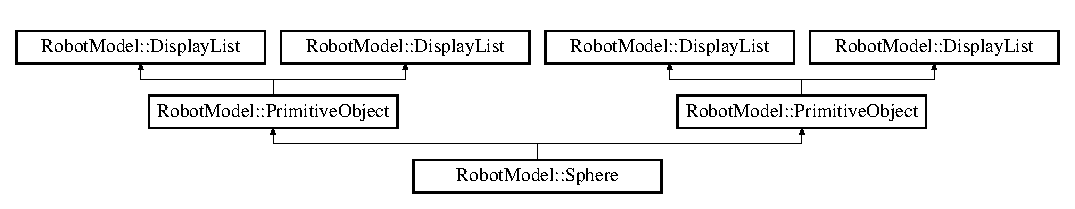
\includegraphics[height=2.35955cm]{class_robot_model_1_1_sphere}
\end{center}
\end{figure}
\subsection*{Public Member Functions}
\begin{DoxyCompactItemize}
\item 
\hyperlink{class_robot_model_1_1_sphere_a9944239ac9fc56091f17701f547652da}{Sphere} (qreal radius, int lod=3)
\item 
virtual \hyperlink{class_robot_model_1_1_sphere_a569c071e50a3e11f678630ee1a17737e}{$\sim$Sphere} ()
\item 
void \hyperlink{class_robot_model_1_1_sphere_a838b5ae4f743aabe24a255dd61d2843c}{makeDisplayList} ()
\item 
\hyperlink{class_robot_model_1_1_sphere_a0a673e3782cc9d061c0f421b2970b4a6}{Sphere} (qreal radius, int lod=3)
\item 
virtual \hyperlink{class_robot_model_1_1_sphere_a19b5af03f0c3f6b28db4d741cbaf5c17}{$\sim$Sphere} ()
\item 
void \hyperlink{class_robot_model_1_1_sphere_a0f338501410a9d8e220ff20ce073d244}{makeDisplayList} ()
\end{DoxyCompactItemize}


\subsection{Constructor \& Destructor Documentation}
\hypertarget{class_robot_model_1_1_sphere_a9944239ac9fc56091f17701f547652da}{
\index{RobotModel::Sphere@{RobotModel::Sphere}!Sphere@{Sphere}}
\index{Sphere@{Sphere}!RobotModel::Sphere@{RobotModel::Sphere}}
\subsubsection[{Sphere}]{\setlength{\rightskip}{0pt plus 5cm}Sphere::Sphere (qreal {\em radius}, \/  int {\em lod} = {\ttfamily 3})}}
\label{class_robot_model_1_1_sphere_a9944239ac9fc56091f17701f547652da}
\hypertarget{class_robot_model_1_1_sphere_a569c071e50a3e11f678630ee1a17737e}{
\index{RobotModel::Sphere@{RobotModel::Sphere}!$\sim$Sphere@{$\sim$Sphere}}
\index{$\sim$Sphere@{$\sim$Sphere}!RobotModel::Sphere@{RobotModel::Sphere}}
\subsubsection[{$\sim$Sphere}]{\setlength{\rightskip}{0pt plus 5cm}Sphere::$\sim$Sphere ()\hspace{0.3cm}{\ttfamily  \mbox{[}virtual\mbox{]}}}}
\label{class_robot_model_1_1_sphere_a569c071e50a3e11f678630ee1a17737e}
\hypertarget{class_robot_model_1_1_sphere_a0a673e3782cc9d061c0f421b2970b4a6}{
\index{RobotModel::Sphere@{RobotModel::Sphere}!Sphere@{Sphere}}
\index{Sphere@{Sphere}!RobotModel::Sphere@{RobotModel::Sphere}}
\subsubsection[{Sphere}]{\setlength{\rightskip}{0pt plus 5cm}RobotModel::Sphere::Sphere (qreal {\em radius}, \/  int {\em lod} = {\ttfamily 3})}}
\label{class_robot_model_1_1_sphere_a0a673e3782cc9d061c0f421b2970b4a6}
\hypertarget{class_robot_model_1_1_sphere_a19b5af03f0c3f6b28db4d741cbaf5c17}{
\index{RobotModel::Sphere@{RobotModel::Sphere}!$\sim$Sphere@{$\sim$Sphere}}
\index{$\sim$Sphere@{$\sim$Sphere}!RobotModel::Sphere@{RobotModel::Sphere}}
\subsubsection[{$\sim$Sphere}]{\setlength{\rightskip}{0pt plus 5cm}virtual RobotModel::Sphere::$\sim$Sphere ()\hspace{0.3cm}{\ttfamily  \mbox{[}virtual\mbox{]}}}}
\label{class_robot_model_1_1_sphere_a19b5af03f0c3f6b28db4d741cbaf5c17}


\subsection{Member Function Documentation}
\hypertarget{class_robot_model_1_1_sphere_a0f338501410a9d8e220ff20ce073d244}{
\index{RobotModel::Sphere@{RobotModel::Sphere}!makeDisplayList@{makeDisplayList}}
\index{makeDisplayList@{makeDisplayList}!RobotModel::Sphere@{RobotModel::Sphere}}
\subsubsection[{makeDisplayList}]{\setlength{\rightskip}{0pt plus 5cm}void RobotModel::Sphere::makeDisplayList ()\hspace{0.3cm}{\ttfamily  \mbox{[}virtual\mbox{]}}}}
\label{class_robot_model_1_1_sphere_a0f338501410a9d8e220ff20ce073d244}


Implements \hyperlink{class_robot_model_1_1_display_list_a842de97924298c7363e50aebd69e5a50}{RobotModel::DisplayList}.\hypertarget{class_robot_model_1_1_sphere_a838b5ae4f743aabe24a255dd61d2843c}{
\index{RobotModel::Sphere@{RobotModel::Sphere}!makeDisplayList@{makeDisplayList}}
\index{makeDisplayList@{makeDisplayList}!RobotModel::Sphere@{RobotModel::Sphere}}
\subsubsection[{makeDisplayList}]{\setlength{\rightskip}{0pt plus 5cm}void Sphere::makeDisplayList ()\hspace{0.3cm}{\ttfamily  \mbox{[}virtual\mbox{]}}}}
\label{class_robot_model_1_1_sphere_a838b5ae4f743aabe24a255dd61d2843c}


Implements \hyperlink{class_robot_model_1_1_display_list_a842de97924298c7363e50aebd69e5a50}{RobotModel::DisplayList}.

The documentation for this class was generated from the following files:\begin{DoxyCompactItemize}
\item 
/Users/kail/imClever/dev/virtualSkin/include/robotModel/\hyperlink{include_2robot_model_2sphere_8h}{sphere.h}\item 
/Users/kail/imClever/dev/virtualSkin/src/robotModel/\hyperlink{src_2robot_model_2sphere_8h}{sphere.h}\item 
/Users/kail/imClever/dev/virtualSkin/src/robotModel/\hyperlink{sphere_8cpp}{sphere.cpp}\end{DoxyCompactItemize}

\hypertarget{class_state_observer}{
\section{StateObserver Class Reference}
\label{class_state_observer}\index{StateObserver@{StateObserver}}
}


{\ttfamily \#include $<$StateObserver.h$>$}Inheritance diagram for StateObserver::\begin{figure}[H]
\begin{center}
\leavevmode
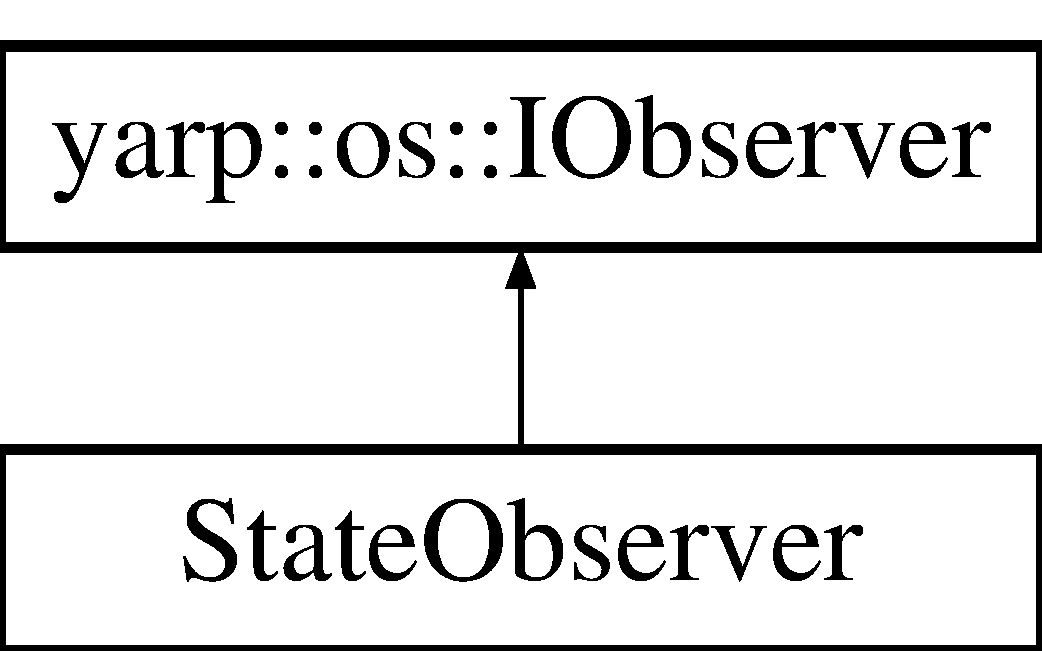
\includegraphics[height=2cm]{class_state_observer}
\end{center}
\end{figure}
\subsection*{Public Member Functions}
\begin{DoxyCompactItemize}
\item 
\hyperlink{class_state_observer_a2c4bfeb55e24f75987cadadc3f89ecca}{StateObserver} (\hyperlink{class_robot_filter}{RobotFilter} $\ast$f, const int b)
\item 
virtual \hyperlink{class_state_observer_af4bf0f323eff464401227a01db686edb}{$\sim$StateObserver} ()
\item 
virtual void \hyperlink{class_state_observer_af104fa553abf31754d9acc084e9aa31f}{onDataObserved} (yarp::os::Bottle \&b)
\item 
QVector$<$ qreal $>$ \hyperlink{class_state_observer_ac77f03f2f6c059e03cb1d5553a4e645d}{nonCollidingPose} ()
\item 
QVector$<$ qreal $>$ \hyperlink{class_state_observer_afe5862adf3afcea5598258625c5db003}{currentPose} ()
\item 
void \hyperlink{class_state_observer_ab41baf5be5f7486796adbbdc0014985b}{initPoseBuffer} (const QVector$<$ qreal $>$ \&v)
\end{DoxyCompactItemize}


\subsection{Constructor \& Destructor Documentation}
\hypertarget{class_state_observer_a2c4bfeb55e24f75987cadadc3f89ecca}{
\index{StateObserver@{StateObserver}!StateObserver@{StateObserver}}
\index{StateObserver@{StateObserver}!StateObserver@{StateObserver}}
\subsubsection[{StateObserver}]{\setlength{\rightskip}{0pt plus 5cm}StateObserver::StateObserver ({\bf RobotFilter} $\ast$ {\em f}, \/  const int {\em b})}}
\label{class_state_observer_a2c4bfeb55e24f75987cadadc3f89ecca}
\hypertarget{class_state_observer_af4bf0f323eff464401227a01db686edb}{
\index{StateObserver@{StateObserver}!$\sim$StateObserver@{$\sim$StateObserver}}
\index{$\sim$StateObserver@{$\sim$StateObserver}!StateObserver@{StateObserver}}
\subsubsection[{$\sim$StateObserver}]{\setlength{\rightskip}{0pt plus 5cm}StateObserver::$\sim$StateObserver ()\hspace{0.3cm}{\ttfamily  \mbox{[}virtual\mbox{]}}}}
\label{class_state_observer_af4bf0f323eff464401227a01db686edb}


\subsection{Member Function Documentation}
\hypertarget{class_state_observer_afe5862adf3afcea5598258625c5db003}{
\index{StateObserver@{StateObserver}!currentPose@{currentPose}}
\index{currentPose@{currentPose}!StateObserver@{StateObserver}}
\subsubsection[{currentPose}]{\setlength{\rightskip}{0pt plus 5cm}QVector$<$qreal$>$ StateObserver::currentPose ()\hspace{0.3cm}{\ttfamily  \mbox{[}inline\mbox{]}}}}
\label{class_state_observer_afe5862adf3afcea5598258625c5db003}
\hypertarget{class_state_observer_ab41baf5be5f7486796adbbdc0014985b}{
\index{StateObserver@{StateObserver}!initPoseBuffer@{initPoseBuffer}}
\index{initPoseBuffer@{initPoseBuffer}!StateObserver@{StateObserver}}
\subsubsection[{initPoseBuffer}]{\setlength{\rightskip}{0pt plus 5cm}void StateObserver::initPoseBuffer (const QVector$<$ qreal $>$ \& {\em v})\hspace{0.3cm}{\ttfamily  \mbox{[}inline\mbox{]}}}}
\label{class_state_observer_ab41baf5be5f7486796adbbdc0014985b}
\hypertarget{class_state_observer_ac77f03f2f6c059e03cb1d5553a4e645d}{
\index{StateObserver@{StateObserver}!nonCollidingPose@{nonCollidingPose}}
\index{nonCollidingPose@{nonCollidingPose}!StateObserver@{StateObserver}}
\subsubsection[{nonCollidingPose}]{\setlength{\rightskip}{0pt plus 5cm}QVector$<$qreal$>$ StateObserver::nonCollidingPose ()\hspace{0.3cm}{\ttfamily  \mbox{[}inline\mbox{]}}}}
\label{class_state_observer_ac77f03f2f6c059e03cb1d5553a4e645d}
\hypertarget{class_state_observer_af104fa553abf31754d9acc084e9aa31f}{
\index{StateObserver@{StateObserver}!onDataObserved@{onDataObserved}}
\index{onDataObserved@{onDataObserved}!StateObserver@{StateObserver}}
\subsubsection[{onDataObserved}]{\setlength{\rightskip}{0pt plus 5cm}void StateObserver::onDataObserved (yarp::os::Bottle \& {\em b})\hspace{0.3cm}{\ttfamily  \mbox{[}virtual\mbox{]}}}}
\label{class_state_observer_af104fa553abf31754d9acc084e9aa31f}
This function is called by filters to inform the implementing objects on data flowing in or out a the calling filter (RpcFilter as well as StreamFilter). 

Implements \hyperlink{classyarp_1_1os_1_1_i_observer_a4829e5a6f2ba6666b9539a4a30f20790}{yarp::os::IObserver}.

The documentation for this class was generated from the following files:\begin{DoxyCompactItemize}
\item 
/Users/kail/imClever/dev/virtualSkin/src/reflex/\hyperlink{_state_observer_8h}{StateObserver.h}\item 
/Users/kail/imClever/dev/virtualSkin/src/reflex/\hyperlink{_state_observer_8cpp}{StateObserver.cpp}\end{DoxyCompactItemize}

\hypertarget{classyarp_1_1os_1_1_stream_filter}{
\section{yarp::os::StreamFilter Class Reference}
\label{classyarp_1_1os_1_1_stream_filter}\index{yarp::os::StreamFilter@{yarp::os::StreamFilter}}
}


{\ttfamily \#include $<$StreamFilter.h$>$}\subsection*{Public Member Functions}
\begin{DoxyCompactItemize}
\item 
\hyperlink{classyarp_1_1os_1_1_stream_filter_a687a3082652cb3163619fa04bfe9db1f}{StreamFilter} ()
\item 
virtual \hyperlink{classyarp_1_1os_1_1_stream_filter_a39cc5195a93b8146c2f9117298f97581}{$\sim$StreamFilter} ()
\item 
bool \hyperlink{classyarp_1_1os_1_1_stream_filter_aa2203de7321cabb2eb8e8a28b66cc470}{open} (ConstString inPortName, ConstString outPortName)
\item 
void \hyperlink{classyarp_1_1os_1_1_stream_filter_a833b30281a0c6039cdfcded6986fe36e}{close} ()
\item 
void \hyperlink{classyarp_1_1os_1_1_stream_filter_a3c72e672f88e6f9e8d77f7af8bcd31ee}{cutConnection} (bool cut=true)
\item 
void \hyperlink{classyarp_1_1os_1_1_stream_filter_a6f911f0b7818d212d58f05fe82c096a1}{setObserver} (\hyperlink{classyarp_1_1os_1_1_i_observer}{IObserver} $\ast$o)
\item 
void \hyperlink{classyarp_1_1os_1_1_stream_filter_a0dad0b2389fa998afc9336509569a01f}{injectData} (const Bottle \&b)
\item 
\hyperlink{classyarp_1_1os_1_1_stream_filter_aa60e6108b7ab7a492d2265a00fe09773}{StreamFilter} ()
\item 
virtual \hyperlink{classyarp_1_1os_1_1_stream_filter_a024da71ac25badd8895898bc057e3488}{$\sim$StreamFilter} ()
\item 
bool \hyperlink{classyarp_1_1os_1_1_stream_filter_a0e0fdc84804bc82ae32c1100d8ad19db}{open} (ConstString inPortName, ConstString outPortName)
\item 
void \hyperlink{classyarp_1_1os_1_1_stream_filter_aaa31b9321ff08b6122a037b3d721e2d4}{close} ()
\item 
void \hyperlink{classyarp_1_1os_1_1_stream_filter_a1f9ef00b6c094c9489121143a4e38c77}{cutConnection} (bool cut=true)
\item 
void \hyperlink{classyarp_1_1os_1_1_stream_filter_a9e7a3182eaf634a5e80e55411c5019b9}{setObserver} (\hyperlink{classyarp_1_1os_1_1_i_observer}{IObserver} $\ast$o)
\item 
void \hyperlink{classyarp_1_1os_1_1_stream_filter_a86214ed7527aca2157153c2ee3899afd}{injectData} (const Bottle \&b)
\end{DoxyCompactItemize}


\subsection{Constructor \& Destructor Documentation}
\hypertarget{classyarp_1_1os_1_1_stream_filter_a687a3082652cb3163619fa04bfe9db1f}{
\index{yarp::os::StreamFilter@{yarp::os::StreamFilter}!StreamFilter@{StreamFilter}}
\index{StreamFilter@{StreamFilter}!yarp::os::StreamFilter@{yarp::os::StreamFilter}}
\subsubsection[{StreamFilter}]{\setlength{\rightskip}{0pt plus 5cm}StreamFilter::StreamFilter ()}}
\label{classyarp_1_1os_1_1_stream_filter_a687a3082652cb3163619fa04bfe9db1f}
\hypertarget{classyarp_1_1os_1_1_stream_filter_a39cc5195a93b8146c2f9117298f97581}{
\index{yarp::os::StreamFilter@{yarp::os::StreamFilter}!$\sim$StreamFilter@{$\sim$StreamFilter}}
\index{$\sim$StreamFilter@{$\sim$StreamFilter}!yarp::os::StreamFilter@{yarp::os::StreamFilter}}
\subsubsection[{$\sim$StreamFilter}]{\setlength{\rightskip}{0pt plus 5cm}StreamFilter::$\sim$StreamFilter ()\hspace{0.3cm}{\ttfamily  \mbox{[}virtual\mbox{]}}}}
\label{classyarp_1_1os_1_1_stream_filter_a39cc5195a93b8146c2f9117298f97581}
\hypertarget{classyarp_1_1os_1_1_stream_filter_aa60e6108b7ab7a492d2265a00fe09773}{
\index{yarp::os::StreamFilter@{yarp::os::StreamFilter}!StreamFilter@{StreamFilter}}
\index{StreamFilter@{StreamFilter}!yarp::os::StreamFilter@{yarp::os::StreamFilter}}
\subsubsection[{StreamFilter}]{\setlength{\rightskip}{0pt plus 5cm}yarp::os::StreamFilter::StreamFilter ()}}
\label{classyarp_1_1os_1_1_stream_filter_aa60e6108b7ab7a492d2265a00fe09773}
\hypertarget{classyarp_1_1os_1_1_stream_filter_a024da71ac25badd8895898bc057e3488}{
\index{yarp::os::StreamFilter@{yarp::os::StreamFilter}!$\sim$StreamFilter@{$\sim$StreamFilter}}
\index{$\sim$StreamFilter@{$\sim$StreamFilter}!yarp::os::StreamFilter@{yarp::os::StreamFilter}}
\subsubsection[{$\sim$StreamFilter}]{\setlength{\rightskip}{0pt plus 5cm}virtual yarp::os::StreamFilter::$\sim$StreamFilter ()\hspace{0.3cm}{\ttfamily  \mbox{[}virtual\mbox{]}}}}
\label{classyarp_1_1os_1_1_stream_filter_a024da71ac25badd8895898bc057e3488}


\subsection{Member Function Documentation}
\hypertarget{classyarp_1_1os_1_1_stream_filter_aaa31b9321ff08b6122a037b3d721e2d4}{
\index{yarp::os::StreamFilter@{yarp::os::StreamFilter}!close@{close}}
\index{close@{close}!yarp::os::StreamFilter@{yarp::os::StreamFilter}}
\subsubsection[{close}]{\setlength{\rightskip}{0pt plus 5cm}void yarp::os::StreamFilter::close ()}}
\label{classyarp_1_1os_1_1_stream_filter_aaa31b9321ff08b6122a037b3d721e2d4}
\hypertarget{classyarp_1_1os_1_1_stream_filter_a833b30281a0c6039cdfcded6986fe36e}{
\index{yarp::os::StreamFilter@{yarp::os::StreamFilter}!close@{close}}
\index{close@{close}!yarp::os::StreamFilter@{yarp::os::StreamFilter}}
\subsubsection[{close}]{\setlength{\rightskip}{0pt plus 5cm}void StreamFilter::close ()}}
\label{classyarp_1_1os_1_1_stream_filter_a833b30281a0c6039cdfcded6986fe36e}
\hypertarget{classyarp_1_1os_1_1_stream_filter_a1f9ef00b6c094c9489121143a4e38c77}{
\index{yarp::os::StreamFilter@{yarp::os::StreamFilter}!cutConnection@{cutConnection}}
\index{cutConnection@{cutConnection}!yarp::os::StreamFilter@{yarp::os::StreamFilter}}
\subsubsection[{cutConnection}]{\setlength{\rightskip}{0pt plus 5cm}void yarp::os::StreamFilter::cutConnection (bool {\em cut} = {\ttfamily true})}}
\label{classyarp_1_1os_1_1_stream_filter_a1f9ef00b6c094c9489121143a4e38c77}
\hypertarget{classyarp_1_1os_1_1_stream_filter_a3c72e672f88e6f9e8d77f7af8bcd31ee}{
\index{yarp::os::StreamFilter@{yarp::os::StreamFilter}!cutConnection@{cutConnection}}
\index{cutConnection@{cutConnection}!yarp::os::StreamFilter@{yarp::os::StreamFilter}}
\subsubsection[{cutConnection}]{\setlength{\rightskip}{0pt plus 5cm}void StreamFilter::cutConnection (bool {\em cut} = {\ttfamily true})}}
\label{classyarp_1_1os_1_1_stream_filter_a3c72e672f88e6f9e8d77f7af8bcd31ee}
\hypertarget{classyarp_1_1os_1_1_stream_filter_a86214ed7527aca2157153c2ee3899afd}{
\index{yarp::os::StreamFilter@{yarp::os::StreamFilter}!injectData@{injectData}}
\index{injectData@{injectData}!yarp::os::StreamFilter@{yarp::os::StreamFilter}}
\subsubsection[{injectData}]{\setlength{\rightskip}{0pt plus 5cm}void yarp::os::StreamFilter::injectData (const Bottle \& {\em b})}}
\label{classyarp_1_1os_1_1_stream_filter_a86214ed7527aca2157153c2ee3899afd}
\hypertarget{classyarp_1_1os_1_1_stream_filter_a0dad0b2389fa998afc9336509569a01f}{
\index{yarp::os::StreamFilter@{yarp::os::StreamFilter}!injectData@{injectData}}
\index{injectData@{injectData}!yarp::os::StreamFilter@{yarp::os::StreamFilter}}
\subsubsection[{injectData}]{\setlength{\rightskip}{0pt plus 5cm}void StreamFilter::injectData (const Bottle \& {\em b})}}
\label{classyarp_1_1os_1_1_stream_filter_a0dad0b2389fa998afc9336509569a01f}
\hypertarget{classyarp_1_1os_1_1_stream_filter_a0e0fdc84804bc82ae32c1100d8ad19db}{
\index{yarp::os::StreamFilter@{yarp::os::StreamFilter}!open@{open}}
\index{open@{open}!yarp::os::StreamFilter@{yarp::os::StreamFilter}}
\subsubsection[{open}]{\setlength{\rightskip}{0pt plus 5cm}bool yarp::os::StreamFilter::open (ConstString {\em inPortName}, \/  ConstString {\em outPortName})}}
\label{classyarp_1_1os_1_1_stream_filter_a0e0fdc84804bc82ae32c1100d8ad19db}
\hypertarget{classyarp_1_1os_1_1_stream_filter_aa2203de7321cabb2eb8e8a28b66cc470}{
\index{yarp::os::StreamFilter@{yarp::os::StreamFilter}!open@{open}}
\index{open@{open}!yarp::os::StreamFilter@{yarp::os::StreamFilter}}
\subsubsection[{open}]{\setlength{\rightskip}{0pt plus 5cm}bool StreamFilter::open (ConstString {\em inPortName}, \/  ConstString {\em outPortName})}}
\label{classyarp_1_1os_1_1_stream_filter_aa2203de7321cabb2eb8e8a28b66cc470}
\hypertarget{classyarp_1_1os_1_1_stream_filter_a9e7a3182eaf634a5e80e55411c5019b9}{
\index{yarp::os::StreamFilter@{yarp::os::StreamFilter}!setObserver@{setObserver}}
\index{setObserver@{setObserver}!yarp::os::StreamFilter@{yarp::os::StreamFilter}}
\subsubsection[{setObserver}]{\setlength{\rightskip}{0pt plus 5cm}void yarp::os::StreamFilter::setObserver ({\bf IObserver} $\ast$ {\em o})}}
\label{classyarp_1_1os_1_1_stream_filter_a9e7a3182eaf634a5e80e55411c5019b9}
\hypertarget{classyarp_1_1os_1_1_stream_filter_a6f911f0b7818d212d58f05fe82c096a1}{
\index{yarp::os::StreamFilter@{yarp::os::StreamFilter}!setObserver@{setObserver}}
\index{setObserver@{setObserver}!yarp::os::StreamFilter@{yarp::os::StreamFilter}}
\subsubsection[{setObserver}]{\setlength{\rightskip}{0pt plus 5cm}void StreamFilter::setObserver ({\bf IObserver} $\ast$ {\em o})}}
\label{classyarp_1_1os_1_1_stream_filter_a6f911f0b7818d212d58f05fe82c096a1}


The documentation for this class was generated from the following files:\begin{DoxyCompactItemize}
\item 
/Users/kail/imClever/dev/virtualSkin/include/yarp/os/\hyperlink{include_2yarp_2os_2_stream_filter_8h}{StreamFilter.h}\item 
/Users/kail/imClever/dev/virtualSkin/src/yarpUtil/gregorFilter/yarp/os/\hyperlink{src_2yarp_util_2gregor_filter_2yarp_2os_2_stream_filter_8h}{StreamFilter.h}\item 
/Users/kail/imClever/dev/virtualSkin/src/yarpUtil/gregorFilter/\hyperlink{_stream_filter_8cpp}{StreamFilter.cpp}\end{DoxyCompactItemize}

\hypertarget{classyarp_1_1os_1_1impl_1_1_stream_filter_impl}{
\section{yarp::os::impl::StreamFilterImpl Class Reference}
\label{classyarp_1_1os_1_1impl_1_1_stream_filter_impl}\index{yarp::os::impl::StreamFilterImpl@{yarp::os::impl::StreamFilterImpl}}
}


{\ttfamily \#include $<$StreamFilterImpl.h$>$}\subsection*{Public Member Functions}
\begin{DoxyCompactItemize}
\item 
\hyperlink{classyarp_1_1os_1_1impl_1_1_stream_filter_impl_a34b63ca7d32244a7c0ec974ce7d3c2f2}{StreamFilterImpl} ()
\item 
virtual \hyperlink{classyarp_1_1os_1_1impl_1_1_stream_filter_impl_a57728d60fe69bb2946135cbc817e6400}{$\sim$StreamFilterImpl} ()
\item 
bool \hyperlink{classyarp_1_1os_1_1impl_1_1_stream_filter_impl_a89e921dc1fa47bc6136bc3135e89ae03}{open} (ConstString outPortName)
\item 
void \hyperlink{classyarp_1_1os_1_1impl_1_1_stream_filter_impl_afe2c98307b0051805788c690b160b977}{close} ()
\item 
void \hyperlink{classyarp_1_1os_1_1impl_1_1_stream_filter_impl_a9a7a37fe9ac8b71cc7a6a54a118617fc}{cutConnection} (bool cut=true)
\item 
void \hyperlink{classyarp_1_1os_1_1impl_1_1_stream_filter_impl_a269889b1cdc1992968861e49d7542e5d}{setObserver} (\hyperlink{classyarp_1_1os_1_1_i_observer}{IObserver} $\ast$o)
\item 
void \hyperlink{classyarp_1_1os_1_1impl_1_1_stream_filter_impl_a114406a0f5eb4ae4c002a76f998e89b2}{injectData} (const Bottle \&b)
\item 
virtual void \hyperlink{classyarp_1_1os_1_1impl_1_1_stream_filter_impl_a9ffe25ea43e69bcc50d3334fea26fff5}{onRead} (Bottle \&b)
\item 
\hyperlink{classyarp_1_1os_1_1impl_1_1_stream_filter_impl_a9db10175fac8a0e45ecdc03c2c57a5be}{StreamFilterImpl} ()
\item 
virtual \hyperlink{classyarp_1_1os_1_1impl_1_1_stream_filter_impl_aa7fa903f6a608c621e892a21f0c0c4eb}{$\sim$StreamFilterImpl} ()
\item 
bool \hyperlink{classyarp_1_1os_1_1impl_1_1_stream_filter_impl_addabbbd78373c7aa7e4712776064891e}{open} (ConstString outPortName)
\item 
void \hyperlink{classyarp_1_1os_1_1impl_1_1_stream_filter_impl_ad7161adcaae840c0f88c7d24312b774f}{close} ()
\item 
void \hyperlink{classyarp_1_1os_1_1impl_1_1_stream_filter_impl_a48096e050f252e896ad831a12da0c6b3}{cutConnection} (bool cut=true)
\item 
void \hyperlink{classyarp_1_1os_1_1impl_1_1_stream_filter_impl_aa3486d2806b76cf08b4594a1a0b367d7}{setObserver} (\hyperlink{classyarp_1_1os_1_1_i_observer}{IObserver} $\ast$o)
\item 
void \hyperlink{classyarp_1_1os_1_1impl_1_1_stream_filter_impl_af1701f0821906931c9271e9561988784}{injectData} (const Bottle \&b)
\item 
virtual void \hyperlink{classyarp_1_1os_1_1impl_1_1_stream_filter_impl_a6124d272f1dedaf326deef524e23a2f9}{onRead} (Bottle \&b)
\end{DoxyCompactItemize}


\subsection{Detailed Description}
Implementation details for the {\ttfamily \hyperlink{classyarp_1_1os_1_1_stream_filter}{StreamFilter}} class. The provided services implement the inner workings of StreamFilters.

\begin{DoxySeeAlso}{See also}
\hyperlink{classyarp_1_1os_1_1_stream_filter}{StreamFilter}
\end{DoxySeeAlso}
\begin{DoxyAttention}{Attention}
This class is not intended to be used by regular users of YARP! 
\end{DoxyAttention}


\subsection{Constructor \& Destructor Documentation}
\hypertarget{classyarp_1_1os_1_1impl_1_1_stream_filter_impl_a34b63ca7d32244a7c0ec974ce7d3c2f2}{
\index{yarp::os::impl::StreamFilterImpl@{yarp::os::impl::StreamFilterImpl}!StreamFilterImpl@{StreamFilterImpl}}
\index{StreamFilterImpl@{StreamFilterImpl}!yarp::os::impl::StreamFilterImpl@{yarp::os::impl::StreamFilterImpl}}
\subsubsection[{StreamFilterImpl}]{\setlength{\rightskip}{0pt plus 5cm}StreamFilterImpl::StreamFilterImpl ()}}
\label{classyarp_1_1os_1_1impl_1_1_stream_filter_impl_a34b63ca7d32244a7c0ec974ce7d3c2f2}
\begin{Desc}
\item[\hyperlink{todo__todo000004}{Todo}]Describe state of a newly created instance \end{Desc}
\hypertarget{classyarp_1_1os_1_1impl_1_1_stream_filter_impl_a57728d60fe69bb2946135cbc817e6400}{
\index{yarp::os::impl::StreamFilterImpl@{yarp::os::impl::StreamFilterImpl}!$\sim$StreamFilterImpl@{$\sim$StreamFilterImpl}}
\index{$\sim$StreamFilterImpl@{$\sim$StreamFilterImpl}!yarp::os::impl::StreamFilterImpl@{yarp::os::impl::StreamFilterImpl}}
\subsubsection[{$\sim$StreamFilterImpl}]{\setlength{\rightskip}{0pt plus 5cm}StreamFilterImpl::$\sim$StreamFilterImpl ()\hspace{0.3cm}{\ttfamily  \mbox{[}virtual\mbox{]}}}}
\label{classyarp_1_1os_1_1impl_1_1_stream_filter_impl_a57728d60fe69bb2946135cbc817e6400}
\hypertarget{classyarp_1_1os_1_1impl_1_1_stream_filter_impl_a9db10175fac8a0e45ecdc03c2c57a5be}{
\index{yarp::os::impl::StreamFilterImpl@{yarp::os::impl::StreamFilterImpl}!StreamFilterImpl@{StreamFilterImpl}}
\index{StreamFilterImpl@{StreamFilterImpl}!yarp::os::impl::StreamFilterImpl@{yarp::os::impl::StreamFilterImpl}}
\subsubsection[{StreamFilterImpl}]{\setlength{\rightskip}{0pt plus 5cm}yarp::os::impl::StreamFilterImpl::StreamFilterImpl ()}}
\label{classyarp_1_1os_1_1impl_1_1_stream_filter_impl_a9db10175fac8a0e45ecdc03c2c57a5be}
\begin{Desc}
\item[\hyperlink{todo__todo000014}{Todo}]Describe state of a newly created instance \end{Desc}
\hypertarget{classyarp_1_1os_1_1impl_1_1_stream_filter_impl_aa7fa903f6a608c621e892a21f0c0c4eb}{
\index{yarp::os::impl::StreamFilterImpl@{yarp::os::impl::StreamFilterImpl}!$\sim$StreamFilterImpl@{$\sim$StreamFilterImpl}}
\index{$\sim$StreamFilterImpl@{$\sim$StreamFilterImpl}!yarp::os::impl::StreamFilterImpl@{yarp::os::impl::StreamFilterImpl}}
\subsubsection[{$\sim$StreamFilterImpl}]{\setlength{\rightskip}{0pt plus 5cm}virtual yarp::os::impl::StreamFilterImpl::$\sim$StreamFilterImpl ()\hspace{0.3cm}{\ttfamily  \mbox{[}virtual\mbox{]}}}}
\label{classyarp_1_1os_1_1impl_1_1_stream_filter_impl_aa7fa903f6a608c621e892a21f0c0c4eb}


\subsection{Member Function Documentation}
\hypertarget{classyarp_1_1os_1_1impl_1_1_stream_filter_impl_ad7161adcaae840c0f88c7d24312b774f}{
\index{yarp::os::impl::StreamFilterImpl@{yarp::os::impl::StreamFilterImpl}!close@{close}}
\index{close@{close}!yarp::os::impl::StreamFilterImpl@{yarp::os::impl::StreamFilterImpl}}
\subsubsection[{close}]{\setlength{\rightskip}{0pt plus 5cm}void yarp::os::impl::StreamFilterImpl::close ()}}
\label{classyarp_1_1os_1_1impl_1_1_stream_filter_impl_ad7161adcaae840c0f88c7d24312b774f}
\begin{Desc}
\item[\hyperlink{todo__todo000016}{Todo}]Document \end{Desc}
\hypertarget{classyarp_1_1os_1_1impl_1_1_stream_filter_impl_afe2c98307b0051805788c690b160b977}{
\index{yarp::os::impl::StreamFilterImpl@{yarp::os::impl::StreamFilterImpl}!close@{close}}
\index{close@{close}!yarp::os::impl::StreamFilterImpl@{yarp::os::impl::StreamFilterImpl}}
\subsubsection[{close}]{\setlength{\rightskip}{0pt plus 5cm}void StreamFilterImpl::close ()}}
\label{classyarp_1_1os_1_1impl_1_1_stream_filter_impl_afe2c98307b0051805788c690b160b977}
\begin{Desc}
\item[\hyperlink{todo__todo000006}{Todo}]Document \end{Desc}
\hypertarget{classyarp_1_1os_1_1impl_1_1_stream_filter_impl_a48096e050f252e896ad831a12da0c6b3}{
\index{yarp::os::impl::StreamFilterImpl@{yarp::os::impl::StreamFilterImpl}!cutConnection@{cutConnection}}
\index{cutConnection@{cutConnection}!yarp::os::impl::StreamFilterImpl@{yarp::os::impl::StreamFilterImpl}}
\subsubsection[{cutConnection}]{\setlength{\rightskip}{0pt plus 5cm}void yarp::os::impl::StreamFilterImpl::cutConnection (bool {\em cut} = {\ttfamily true})}}
\label{classyarp_1_1os_1_1impl_1_1_stream_filter_impl_a48096e050f252e896ad831a12da0c6b3}
\hypertarget{classyarp_1_1os_1_1impl_1_1_stream_filter_impl_a9a7a37fe9ac8b71cc7a6a54a118617fc}{
\index{yarp::os::impl::StreamFilterImpl@{yarp::os::impl::StreamFilterImpl}!cutConnection@{cutConnection}}
\index{cutConnection@{cutConnection}!yarp::os::impl::StreamFilterImpl@{yarp::os::impl::StreamFilterImpl}}
\subsubsection[{cutConnection}]{\setlength{\rightskip}{0pt plus 5cm}void StreamFilterImpl::cutConnection (bool {\em cut} = {\ttfamily true})}}
\label{classyarp_1_1os_1_1impl_1_1_stream_filter_impl_a9a7a37fe9ac8b71cc7a6a54a118617fc}
\hypertarget{classyarp_1_1os_1_1impl_1_1_stream_filter_impl_af1701f0821906931c9271e9561988784}{
\index{yarp::os::impl::StreamFilterImpl@{yarp::os::impl::StreamFilterImpl}!injectData@{injectData}}
\index{injectData@{injectData}!yarp::os::impl::StreamFilterImpl@{yarp::os::impl::StreamFilterImpl}}
\subsubsection[{injectData}]{\setlength{\rightskip}{0pt plus 5cm}void yarp::os::impl::StreamFilterImpl::injectData (const Bottle \& {\em b})}}
\label{classyarp_1_1os_1_1impl_1_1_stream_filter_impl_af1701f0821906931c9271e9561988784}
\hypertarget{classyarp_1_1os_1_1impl_1_1_stream_filter_impl_a114406a0f5eb4ae4c002a76f998e89b2}{
\index{yarp::os::impl::StreamFilterImpl@{yarp::os::impl::StreamFilterImpl}!injectData@{injectData}}
\index{injectData@{injectData}!yarp::os::impl::StreamFilterImpl@{yarp::os::impl::StreamFilterImpl}}
\subsubsection[{injectData}]{\setlength{\rightskip}{0pt plus 5cm}void StreamFilterImpl::injectData (const Bottle \& {\em b})}}
\label{classyarp_1_1os_1_1impl_1_1_stream_filter_impl_a114406a0f5eb4ae4c002a76f998e89b2}
\hypertarget{classyarp_1_1os_1_1impl_1_1_stream_filter_impl_a6124d272f1dedaf326deef524e23a2f9}{
\index{yarp::os::impl::StreamFilterImpl@{yarp::os::impl::StreamFilterImpl}!onRead@{onRead}}
\index{onRead@{onRead}!yarp::os::impl::StreamFilterImpl@{yarp::os::impl::StreamFilterImpl}}
\subsubsection[{onRead}]{\setlength{\rightskip}{0pt plus 5cm}virtual void yarp::os::impl::StreamFilterImpl::onRead (Bottle \& {\em b})\hspace{0.3cm}{\ttfamily  \mbox{[}virtual\mbox{]}}}}
\label{classyarp_1_1os_1_1impl_1_1_stream_filter_impl_a6124d272f1dedaf326deef524e23a2f9}
\hypertarget{classyarp_1_1os_1_1impl_1_1_stream_filter_impl_a9ffe25ea43e69bcc50d3334fea26fff5}{
\index{yarp::os::impl::StreamFilterImpl@{yarp::os::impl::StreamFilterImpl}!onRead@{onRead}}
\index{onRead@{onRead}!yarp::os::impl::StreamFilterImpl@{yarp::os::impl::StreamFilterImpl}}
\subsubsection[{onRead}]{\setlength{\rightskip}{0pt plus 5cm}void StreamFilterImpl::onRead (Bottle \& {\em b})\hspace{0.3cm}{\ttfamily  \mbox{[}virtual\mbox{]}}}}
\label{classyarp_1_1os_1_1impl_1_1_stream_filter_impl_a9ffe25ea43e69bcc50d3334fea26fff5}
\hypertarget{classyarp_1_1os_1_1impl_1_1_stream_filter_impl_addabbbd78373c7aa7e4712776064891e}{
\index{yarp::os::impl::StreamFilterImpl@{yarp::os::impl::StreamFilterImpl}!open@{open}}
\index{open@{open}!yarp::os::impl::StreamFilterImpl@{yarp::os::impl::StreamFilterImpl}}
\subsubsection[{open}]{\setlength{\rightskip}{0pt plus 5cm}bool yarp::os::impl::StreamFilterImpl::open (ConstString {\em outPortName})}}
\label{classyarp_1_1os_1_1impl_1_1_stream_filter_impl_addabbbd78373c7aa7e4712776064891e}
\begin{Desc}
\item[\hyperlink{todo__todo000015}{Todo}]Document \end{Desc}
\hypertarget{classyarp_1_1os_1_1impl_1_1_stream_filter_impl_a89e921dc1fa47bc6136bc3135e89ae03}{
\index{yarp::os::impl::StreamFilterImpl@{yarp::os::impl::StreamFilterImpl}!open@{open}}
\index{open@{open}!yarp::os::impl::StreamFilterImpl@{yarp::os::impl::StreamFilterImpl}}
\subsubsection[{open}]{\setlength{\rightskip}{0pt plus 5cm}bool StreamFilterImpl::open (ConstString {\em outPortName})}}
\label{classyarp_1_1os_1_1impl_1_1_stream_filter_impl_a89e921dc1fa47bc6136bc3135e89ae03}
\begin{Desc}
\item[\hyperlink{todo__todo000005}{Todo}]Document \end{Desc}
\hypertarget{classyarp_1_1os_1_1impl_1_1_stream_filter_impl_aa3486d2806b76cf08b4594a1a0b367d7}{
\index{yarp::os::impl::StreamFilterImpl@{yarp::os::impl::StreamFilterImpl}!setObserver@{setObserver}}
\index{setObserver@{setObserver}!yarp::os::impl::StreamFilterImpl@{yarp::os::impl::StreamFilterImpl}}
\subsubsection[{setObserver}]{\setlength{\rightskip}{0pt plus 5cm}void yarp::os::impl::StreamFilterImpl::setObserver ({\bf IObserver} $\ast$ {\em o})}}
\label{classyarp_1_1os_1_1impl_1_1_stream_filter_impl_aa3486d2806b76cf08b4594a1a0b367d7}
\hypertarget{classyarp_1_1os_1_1impl_1_1_stream_filter_impl_a269889b1cdc1992968861e49d7542e5d}{
\index{yarp::os::impl::StreamFilterImpl@{yarp::os::impl::StreamFilterImpl}!setObserver@{setObserver}}
\index{setObserver@{setObserver}!yarp::os::impl::StreamFilterImpl@{yarp::os::impl::StreamFilterImpl}}
\subsubsection[{setObserver}]{\setlength{\rightskip}{0pt plus 5cm}void StreamFilterImpl::setObserver ({\bf IObserver} $\ast$ {\em o})}}
\label{classyarp_1_1os_1_1impl_1_1_stream_filter_impl_a269889b1cdc1992968861e49d7542e5d}


The documentation for this class was generated from the following files:\begin{DoxyCompactItemize}
\item 
/Users/kail/imClever/dev/virtualSkin/include/yarp/os/impl/\hyperlink{include_2yarp_2os_2impl_2_stream_filter_impl_8h}{StreamFilterImpl.h}\item 
/Users/kail/imClever/dev/virtualSkin/src/yarpUtil/gregorFilter/yarp/os/impl/\hyperlink{src_2yarp_util_2gregor_filter_2yarp_2os_2impl_2_stream_filter_impl_8h}{StreamFilterImpl.h}\item 
/Users/kail/imClever/dev/virtualSkin/src/yarpUtil/gregorFilter/\hyperlink{_stream_filter_impl_8cpp}{StreamFilterImpl.cpp}\end{DoxyCompactItemize}

\hypertarget{class_robot_model_1_1_world}{
\section{RobotModel::World Class Reference}
\label{class_robot_model_1_1_world}\index{RobotModel::World@{RobotModel::World}}
}


{\ttfamily \#include $<$world.h$>$}Inheritance diagram for RobotModel::World::\begin{figure}[H]
\begin{center}
\leavevmode
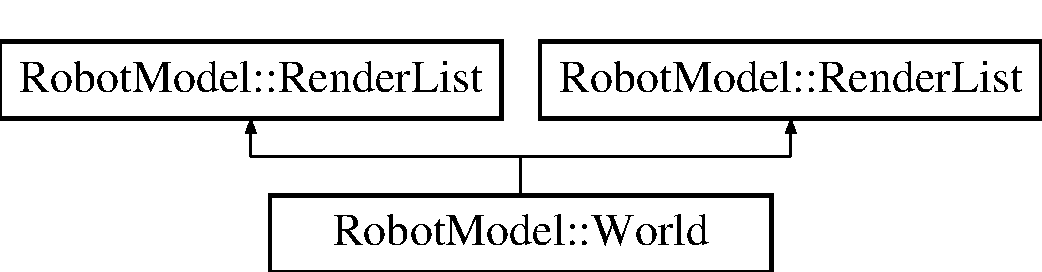
\includegraphics[height=2cm]{class_robot_model_1_1_world}
\end{center}
\end{figure}
\subsection*{Public Member Functions}
\begin{DoxyCompactItemize}
\item 
\hyperlink{class_robot_model_1_1_world_afa39d4e6f714a7a3691ac0c656f5e8a8}{World} ()
\item 
\hyperlink{class_robot_model_1_1_world_a8c73fba541a5817fff65147ba47cd827}{$\sim$World} ()
\item 
\hyperlink{class_robot_model_1_1_composite_object}{CompositeObject} $\ast$ \hyperlink{class_robot_model_1_1_world_af9b942f5df468adf15a285b509bc69e5}{newSphere} (double r, const QVector3D \&pos)
\item 
\hyperlink{class_robot_model_1_1_composite_object}{CompositeObject} $\ast$ \hyperlink{class_robot_model_1_1_world_aee6474d33f4ec03a15fa908f06db9748}{newSSphere} (double r, const QVector3D \&pos)
\item 
\hyperlink{class_robot_model_1_1_composite_object}{CompositeObject} $\ast$ \hyperlink{class_robot_model_1_1_world_a8dd79f7cf657eda9de58181bc9fbb564}{newCylinder} (double r, double h, const QVector3D \&pos)
\item 
\hyperlink{class_robot_model_1_1_composite_object}{CompositeObject} $\ast$ \hyperlink{class_robot_model_1_1_world_a36ee6c4337fbe9097f2bc30a1843cdb5}{newSCylinder} (double r, double h, const QVector3D \&pos)
\item 
\hyperlink{class_robot_model_1_1_composite_object}{CompositeObject} $\ast$ \hyperlink{class_robot_model_1_1_world_a9c100912af0adb5275b73b6660efe475}{newBox} (const QVector3D \&size, const QVector3D \&pos)
\item 
\hyperlink{class_robot_model_1_1_composite_object}{CompositeObject} $\ast$ \hyperlink{class_robot_model_1_1_world_adf2304f9f78471e03d2962b326fe4ce9}{newSBox} (const QVector3D \&size, const QVector3D \&pos)
\item 
\hyperlink{class_robot_model_1_1_composite_object}{CompositeObject} $\ast$ \hyperlink{class_robot_model_1_1_world_a82289c85d931bffc967a90a12e04477a}{newObject} (const QString \&name, const QVector3D \&pos)
\item 
\hyperlink{class_robot_model_1_1_composite_object}{CompositeObject} $\ast$ \hyperlink{class_robot_model_1_1_world_adbfd8acea10b8375ed35c737afd5b929}{append} (\hyperlink{class_robot_model_1_1_composite_object}{CompositeObject} $\ast$obj)
\item 
\hyperlink{class_robot_model_1_1_composite_object}{CompositeObject} $\ast$ \hyperlink{class_robot_model_1_1_world_a2ccf0c4dd817ecae42edbb82f54289a2}{getObjectByName} (const QString \&name)
\item 
bool \hyperlink{class_robot_model_1_1_world_a40f4e4bfed5121602f993bf561932b07}{remove} (\hyperlink{class_robot_model_1_1_composite_object}{CompositeObject} $\ast$object)
\item 
bool \hyperlink{class_robot_model_1_1_world_a498c5d79bc95bd308680c2a8c5e475b0}{removePrimitive} (\hyperlink{class_robot_model_1_1_composite_object}{CompositeObject} $\ast$object, \hyperlink{class_robot_model_1_1_primitive_object}{PrimitiveObject} $\ast$primitive)
\item 
void \hyperlink{class_robot_model_1_1_world_a24f6906f2e4f0c761653a8f9e42588a6}{clear} ()
\item 
void \hyperlink{class_robot_model_1_1_world_a530cb18d1249f7c6e94c4ba6879cf36a}{filterCollisions} (const \hyperlink{class_robot_model_1_1_composite_object}{CompositeObject} $\ast$)
\item 
void \hyperlink{class_robot_model_1_1_world_a38aea4885454231131d4ccb7945138dc}{filterCollisions} (\hyperlink{class_robot_model_1_1_primitive_object}{PrimitiveObject} $\ast$)
\item 
void \hyperlink{class_robot_model_1_1_world_a150eab10c21532162bb698d72aecec16}{render} ()
\item 
void \hyperlink{class_robot_model_1_1_world_a2300046adaa75a432476dbef1934bb01}{notColliding} ()
\end{DoxyCompactItemize}


\subsection{Constructor \& Destructor Documentation}
\hypertarget{class_robot_model_1_1_world_afa39d4e6f714a7a3691ac0c656f5e8a8}{
\index{RobotModel::World@{RobotModel::World}!World@{World}}
\index{World@{World}!RobotModel::World@{RobotModel::World}}
\subsubsection[{World}]{\setlength{\rightskip}{0pt plus 5cm}World::World ()}}
\label{class_robot_model_1_1_world_afa39d4e6f714a7a3691ac0c656f5e8a8}
\hypertarget{class_robot_model_1_1_world_a8c73fba541a5817fff65147ba47cd827}{
\index{RobotModel::World@{RobotModel::World}!$\sim$World@{$\sim$World}}
\index{$\sim$World@{$\sim$World}!RobotModel::World@{RobotModel::World}}
\subsubsection[{$\sim$World}]{\setlength{\rightskip}{0pt plus 5cm}World::$\sim$World ()}}
\label{class_robot_model_1_1_world_a8c73fba541a5817fff65147ba47cd827}


\subsection{Member Function Documentation}
\hypertarget{class_robot_model_1_1_world_adbfd8acea10b8375ed35c737afd5b929}{
\index{RobotModel::World@{RobotModel::World}!append@{append}}
\index{append@{append}!RobotModel::World@{RobotModel::World}}
\subsubsection[{append}]{\setlength{\rightskip}{0pt plus 5cm}{\bf CompositeObject} $\ast$ World::append ({\bf CompositeObject} $\ast$ {\em obj})}}
\label{class_robot_model_1_1_world_adbfd8acea10b8375ed35c737afd5b929}
\hypertarget{class_robot_model_1_1_world_a24f6906f2e4f0c761653a8f9e42588a6}{
\index{RobotModel::World@{RobotModel::World}!clear@{clear}}
\index{clear@{clear}!RobotModel::World@{RobotModel::World}}
\subsubsection[{clear}]{\setlength{\rightskip}{0pt plus 5cm}void World::clear ()}}
\label{class_robot_model_1_1_world_a24f6906f2e4f0c761653a8f9e42588a6}
\hypertarget{class_robot_model_1_1_world_a38aea4885454231131d4ccb7945138dc}{
\index{RobotModel::World@{RobotModel::World}!filterCollisions@{filterCollisions}}
\index{filterCollisions@{filterCollisions}!RobotModel::World@{RobotModel::World}}
\subsubsection[{filterCollisions}]{\setlength{\rightskip}{0pt plus 5cm}void World::filterCollisions ({\bf PrimitiveObject} $\ast$ {\em prim})}}
\label{class_robot_model_1_1_world_a38aea4885454231131d4ccb7945138dc}
\hypertarget{class_robot_model_1_1_world_a530cb18d1249f7c6e94c4ba6879cf36a}{
\index{RobotModel::World@{RobotModel::World}!filterCollisions@{filterCollisions}}
\index{filterCollisions@{filterCollisions}!RobotModel::World@{RobotModel::World}}
\subsubsection[{filterCollisions}]{\setlength{\rightskip}{0pt plus 5cm}void World::filterCollisions (const {\bf CompositeObject} $\ast$ {\em obj})}}
\label{class_robot_model_1_1_world_a530cb18d1249f7c6e94c4ba6879cf36a}
\hypertarget{class_robot_model_1_1_world_a2ccf0c4dd817ecae42edbb82f54289a2}{
\index{RobotModel::World@{RobotModel::World}!getObjectByName@{getObjectByName}}
\index{getObjectByName@{getObjectByName}!RobotModel::World@{RobotModel::World}}
\subsubsection[{getObjectByName}]{\setlength{\rightskip}{0pt plus 5cm}{\bf CompositeObject} $\ast$ World::getObjectByName (const QString \& {\em name})}}
\label{class_robot_model_1_1_world_a2ccf0c4dd817ecae42edbb82f54289a2}
\hypertarget{class_robot_model_1_1_world_a9c100912af0adb5275b73b6660efe475}{
\index{RobotModel::World@{RobotModel::World}!newBox@{newBox}}
\index{newBox@{newBox}!RobotModel::World@{RobotModel::World}}
\subsubsection[{newBox}]{\setlength{\rightskip}{0pt plus 5cm}{\bf CompositeObject} $\ast$ World::newBox (const QVector3D \& {\em size}, \/  const QVector3D \& {\em pos})}}
\label{class_robot_model_1_1_world_a9c100912af0adb5275b73b6660efe475}
\hypertarget{class_robot_model_1_1_world_a8dd79f7cf657eda9de58181bc9fbb564}{
\index{RobotModel::World@{RobotModel::World}!newCylinder@{newCylinder}}
\index{newCylinder@{newCylinder}!RobotModel::World@{RobotModel::World}}
\subsubsection[{newCylinder}]{\setlength{\rightskip}{0pt plus 5cm}{\bf CompositeObject} $\ast$ World::newCylinder (double {\em r}, \/  double {\em h}, \/  const QVector3D \& {\em pos})}}
\label{class_robot_model_1_1_world_a8dd79f7cf657eda9de58181bc9fbb564}
\hypertarget{class_robot_model_1_1_world_a82289c85d931bffc967a90a12e04477a}{
\index{RobotModel::World@{RobotModel::World}!newObject@{newObject}}
\index{newObject@{newObject}!RobotModel::World@{RobotModel::World}}
\subsubsection[{newObject}]{\setlength{\rightskip}{0pt plus 5cm}{\bf CompositeObject} $\ast$ World::newObject (const QString \& {\em name}, \/  const QVector3D \& {\em pos})}}
\label{class_robot_model_1_1_world_a82289c85d931bffc967a90a12e04477a}
\hypertarget{class_robot_model_1_1_world_adf2304f9f78471e03d2962b326fe4ce9}{
\index{RobotModel::World@{RobotModel::World}!newSBox@{newSBox}}
\index{newSBox@{newSBox}!RobotModel::World@{RobotModel::World}}
\subsubsection[{newSBox}]{\setlength{\rightskip}{0pt plus 5cm}{\bf CompositeObject} $\ast$ World::newSBox (const QVector3D \& {\em size}, \/  const QVector3D \& {\em pos})}}
\label{class_robot_model_1_1_world_adf2304f9f78471e03d2962b326fe4ce9}
\hypertarget{class_robot_model_1_1_world_a36ee6c4337fbe9097f2bc30a1843cdb5}{
\index{RobotModel::World@{RobotModel::World}!newSCylinder@{newSCylinder}}
\index{newSCylinder@{newSCylinder}!RobotModel::World@{RobotModel::World}}
\subsubsection[{newSCylinder}]{\setlength{\rightskip}{0pt plus 5cm}{\bf CompositeObject} $\ast$ World::newSCylinder (double {\em r}, \/  double {\em h}, \/  const QVector3D \& {\em pos})}}
\label{class_robot_model_1_1_world_a36ee6c4337fbe9097f2bc30a1843cdb5}
\hypertarget{class_robot_model_1_1_world_af9b942f5df468adf15a285b509bc69e5}{
\index{RobotModel::World@{RobotModel::World}!newSphere@{newSphere}}
\index{newSphere@{newSphere}!RobotModel::World@{RobotModel::World}}
\subsubsection[{newSphere}]{\setlength{\rightskip}{0pt plus 5cm}{\bf CompositeObject} $\ast$ World::newSphere (double {\em r}, \/  const QVector3D \& {\em pos})}}
\label{class_robot_model_1_1_world_af9b942f5df468adf15a285b509bc69e5}
\hypertarget{class_robot_model_1_1_world_aee6474d33f4ec03a15fa908f06db9748}{
\index{RobotModel::World@{RobotModel::World}!newSSphere@{newSSphere}}
\index{newSSphere@{newSSphere}!RobotModel::World@{RobotModel::World}}
\subsubsection[{newSSphere}]{\setlength{\rightskip}{0pt plus 5cm}{\bf CompositeObject} $\ast$ World::newSSphere (double {\em r}, \/  const QVector3D \& {\em pos})}}
\label{class_robot_model_1_1_world_aee6474d33f4ec03a15fa908f06db9748}
\hypertarget{class_robot_model_1_1_world_a2300046adaa75a432476dbef1934bb01}{
\index{RobotModel::World@{RobotModel::World}!notColliding@{notColliding}}
\index{notColliding@{notColliding}!RobotModel::World@{RobotModel::World}}
\subsubsection[{notColliding}]{\setlength{\rightskip}{0pt plus 5cm}void World::notColliding ()\hspace{0.3cm}{\ttfamily  \mbox{[}virtual\mbox{]}}}}
\label{class_robot_model_1_1_world_a2300046adaa75a432476dbef1934bb01}


Implements \hyperlink{class_robot_model_1_1_render_list_a78436c997913ce9ad41a9bd1da9b3d96}{RobotModel::RenderList}.\hypertarget{class_robot_model_1_1_world_a40f4e4bfed5121602f993bf561932b07}{
\index{RobotModel::World@{RobotModel::World}!remove@{remove}}
\index{remove@{remove}!RobotModel::World@{RobotModel::World}}
\subsubsection[{remove}]{\setlength{\rightskip}{0pt plus 5cm}bool World::remove ({\bf CompositeObject} $\ast$ {\em object})}}
\label{class_robot_model_1_1_world_a40f4e4bfed5121602f993bf561932b07}
\hypertarget{class_robot_model_1_1_world_a498c5d79bc95bd308680c2a8c5e475b0}{
\index{RobotModel::World@{RobotModel::World}!removePrimitive@{removePrimitive}}
\index{removePrimitive@{removePrimitive}!RobotModel::World@{RobotModel::World}}
\subsubsection[{removePrimitive}]{\setlength{\rightskip}{0pt plus 5cm}bool World::removePrimitive ({\bf CompositeObject} $\ast$ {\em object}, \/  {\bf PrimitiveObject} $\ast$ {\em primitive})}}
\label{class_robot_model_1_1_world_a498c5d79bc95bd308680c2a8c5e475b0}
\hypertarget{class_robot_model_1_1_world_a150eab10c21532162bb698d72aecec16}{
\index{RobotModel::World@{RobotModel::World}!render@{render}}
\index{render@{render}!RobotModel::World@{RobotModel::World}}
\subsubsection[{render}]{\setlength{\rightskip}{0pt plus 5cm}void World::render ()\hspace{0.3cm}{\ttfamily  \mbox{[}virtual\mbox{]}}}}
\label{class_robot_model_1_1_world_a150eab10c21532162bb698d72aecec16}


Implements \hyperlink{class_robot_model_1_1_render_list_ac8646765beee22bf11582049dc3cf195}{RobotModel::RenderList}.

The documentation for this class was generated from the following files:\begin{DoxyCompactItemize}
\item 
/Users/kail/imClever/dev/virtualSkin/src/robotModel/\hyperlink{world_8h}{world.h}\item 
/Users/kail/imClever/dev/virtualSkin/src/robotModel/\hyperlink{world_8cpp}{world.cpp}\end{DoxyCompactItemize}

\hypertarget{class_robot_model_1_1_world_rpc_interface}{
\section{RobotModel::WorldRpcInterface Class Reference}
\label{class_robot_model_1_1_world_rpc_interface}\index{RobotModel::WorldRpcInterface@{RobotModel::WorldRpcInterface}}
}


{\ttfamily \#include $<$worldRpcInterface.h$>$}Inheritance diagram for RobotModel::WorldRpcInterface::\begin{figure}[H]
\begin{center}
\leavevmode
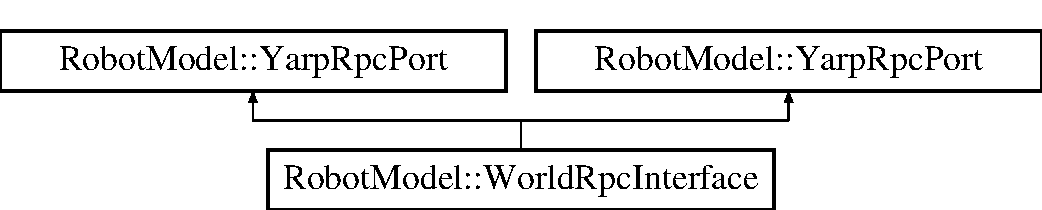
\includegraphics[height=2cm]{class_robot_model_1_1_world_rpc_interface}
\end{center}
\end{figure}
\subsection*{Public Member Functions}
\begin{DoxyCompactItemize}
\item 
\hyperlink{class_robot_model_1_1_world_rpc_interface_a214bbac16ce3a3a94aa1bd600090ae2b}{WorldRpcInterface} ()
\item 
virtual \hyperlink{class_robot_model_1_1_world_rpc_interface_a6b990fdbe2cb39fc2d0e2ef9e8139250}{$\sim$WorldRpcInterface} ()
\item 
void \hyperlink{class_robot_model_1_1_world_rpc_interface_ae5a8361ea49e3bfb4218d7bcfd791587}{setWorld} (\hyperlink{class_robot_model_1_1_world}{World} $\ast$aWorld)
\end{DoxyCompactItemize}


\subsection{Constructor \& Destructor Documentation}
\hypertarget{class_robot_model_1_1_world_rpc_interface_a214bbac16ce3a3a94aa1bd600090ae2b}{
\index{RobotModel::WorldRpcInterface@{RobotModel::WorldRpcInterface}!WorldRpcInterface@{WorldRpcInterface}}
\index{WorldRpcInterface@{WorldRpcInterface}!RobotModel::WorldRpcInterface@{RobotModel::WorldRpcInterface}}
\subsubsection[{WorldRpcInterface}]{\setlength{\rightskip}{0pt plus 5cm}WorldRpcInterface::WorldRpcInterface ()}}
\label{class_robot_model_1_1_world_rpc_interface_a214bbac16ce3a3a94aa1bd600090ae2b}
\hypertarget{class_robot_model_1_1_world_rpc_interface_a6b990fdbe2cb39fc2d0e2ef9e8139250}{
\index{RobotModel::WorldRpcInterface@{RobotModel::WorldRpcInterface}!$\sim$WorldRpcInterface@{$\sim$WorldRpcInterface}}
\index{$\sim$WorldRpcInterface@{$\sim$WorldRpcInterface}!RobotModel::WorldRpcInterface@{RobotModel::WorldRpcInterface}}
\subsubsection[{$\sim$WorldRpcInterface}]{\setlength{\rightskip}{0pt plus 5cm}WorldRpcInterface::$\sim$WorldRpcInterface ()\hspace{0.3cm}{\ttfamily  \mbox{[}virtual\mbox{]}}}}
\label{class_robot_model_1_1_world_rpc_interface_a6b990fdbe2cb39fc2d0e2ef9e8139250}


\subsection{Member Function Documentation}
\hypertarget{class_robot_model_1_1_world_rpc_interface_ae5a8361ea49e3bfb4218d7bcfd791587}{
\index{RobotModel::WorldRpcInterface@{RobotModel::WorldRpcInterface}!setWorld@{setWorld}}
\index{setWorld@{setWorld}!RobotModel::WorldRpcInterface@{RobotModel::WorldRpcInterface}}
\subsubsection[{setWorld}]{\setlength{\rightskip}{0pt plus 5cm}void RobotModel::WorldRpcInterface::setWorld ({\bf World} $\ast$ {\em aWorld})\hspace{0.3cm}{\ttfamily  \mbox{[}inline\mbox{]}}}}
\label{class_robot_model_1_1_world_rpc_interface_ae5a8361ea49e3bfb4218d7bcfd791587}


The documentation for this class was generated from the following files:\begin{DoxyCompactItemize}
\item 
/Users/kail/imClever/dev/virtualSkin/src/yarpUtil/\hyperlink{world_rpc_interface_8h}{worldRpcInterface.h}\item 
/Users/kail/imClever/dev/virtualSkin/src/yarpUtil/\hyperlink{world_rpc_interface_8cpp}{worldRpcInterface.cpp}\end{DoxyCompactItemize}

\hypertarget{class_robot_model_1_1_yarp_rpc_port}{
\section{RobotModel::YarpRpcPort Class Reference}
\label{class_robot_model_1_1_yarp_rpc_port}\index{RobotModel::YarpRpcPort@{RobotModel::YarpRpcPort}}
}


{\ttfamily \#include $<$yarpRpcPort.h$>$}Inheritance diagram for RobotModel::YarpRpcPort::\begin{figure}[H]
\begin{center}
\leavevmode
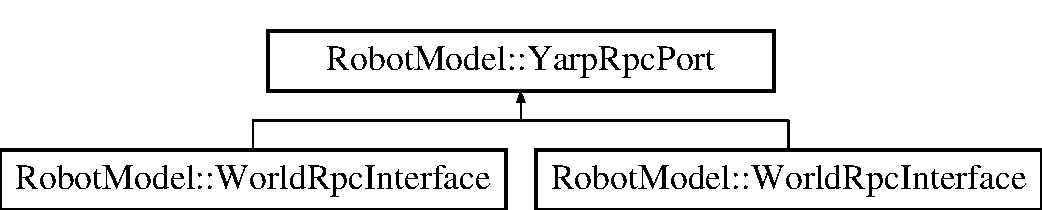
\includegraphics[height=2cm]{class_robot_model_1_1_yarp_rpc_port}
\end{center}
\end{figure}
\subsection*{Public Member Functions}
\begin{DoxyCompactItemize}
\item 
\hyperlink{class_robot_model_1_1_yarp_rpc_port_a393b44f37d77b25d8c5cb7f14609c4d5}{YarpRpcPort} ()
\item 
virtual \hyperlink{class_robot_model_1_1_yarp_rpc_port_acf21bbb8e38b69fd9c3769a2f9b45743}{$\sim$YarpRpcPort} ()
\item 
void \hyperlink{class_robot_model_1_1_yarp_rpc_port_a6fe22d6e8403cb3560964dd31d66c243}{useDebug} ()
\item 
void \hyperlink{class_robot_model_1_1_yarp_rpc_port_a87e299eb43783a25cd71def0e50eb9dc}{noDebug} ()
\item 
void \hyperlink{class_robot_model_1_1_yarp_rpc_port_aa30cabbf5681b128766ad8556c33cd65}{setName} (const QString \&name)
\item 
virtual void \hyperlink{class_robot_model_1_1_yarp_rpc_port_a3e4c1be7ae685d9478b38d71255b1bcd}{run} ()
\item 
virtual bool \hyperlink{class_robot_model_1_1_yarp_rpc_port_a156879aeb8b6641c0f63a6633af8c568}{handler} (const yarp::os::Bottle \&cmd, yarp::os::Bottle \&reply)=0
\item 
void \hyperlink{class_robot_model_1_1_yarp_rpc_port_ae26626cb99ca15bfec5e5162845018c2}{showBottle} (yarp::os::Bottle \&anUnknownBottle, int indentation=0)
\item 
void \hyperlink{class_robot_model_1_1_yarp_rpc_port_a1554e6c2e38cb71f2521280f65bbab05}{stop} ()
\item 
void \hyperlink{class_robot_model_1_1_yarp_rpc_port_a93d242e15bb04534f7db4fe6636a0086}{restart} ()
\item 
\hyperlink{class_robot_model_1_1_yarp_rpc_port_a056dd5174b17abd2a530eb9c77c1badb}{YarpRpcPort} ()
\item 
virtual \hyperlink{class_robot_model_1_1_yarp_rpc_port_acc982a6fdf62ef56ff39bd4ca56375cd}{$\sim$YarpRpcPort} ()
\item 
void \hyperlink{class_robot_model_1_1_yarp_rpc_port_a6fe22d6e8403cb3560964dd31d66c243}{useDebug} ()
\item 
void \hyperlink{class_robot_model_1_1_yarp_rpc_port_a87e299eb43783a25cd71def0e50eb9dc}{noDebug} ()
\item 
void \hyperlink{class_robot_model_1_1_yarp_rpc_port_aa30cabbf5681b128766ad8556c33cd65}{setName} (const QString \&name)
\item 
virtual void \hyperlink{class_robot_model_1_1_yarp_rpc_port_a1d70c28615104cd25ce2d2e7b61a592c}{run} ()
\item 
virtual bool \hyperlink{class_robot_model_1_1_yarp_rpc_port_a156879aeb8b6641c0f63a6633af8c568}{handler} (const yarp::os::Bottle \&cmd, yarp::os::Bottle \&reply)=0
\item 
void \hyperlink{class_robot_model_1_1_yarp_rpc_port_abb0330c695bd22838cee0d2578b66d2d}{showBottle} (yarp::os::Bottle \&anUnknownBottle, int indentation=0)
\item 
void \hyperlink{class_robot_model_1_1_yarp_rpc_port_a7c02179416d26e3e741a385cc1320278}{stop} ()
\item 
void \hyperlink{class_robot_model_1_1_yarp_rpc_port_ac72752818661170c795ed1c4c10dcac2}{restart} ()
\end{DoxyCompactItemize}


\subsection{Constructor \& Destructor Documentation}
\hypertarget{class_robot_model_1_1_yarp_rpc_port_a393b44f37d77b25d8c5cb7f14609c4d5}{
\index{RobotModel::YarpRpcPort@{RobotModel::YarpRpcPort}!YarpRpcPort@{YarpRpcPort}}
\index{YarpRpcPort@{YarpRpcPort}!RobotModel::YarpRpcPort@{RobotModel::YarpRpcPort}}
\subsubsection[{YarpRpcPort}]{\setlength{\rightskip}{0pt plus 5cm}YarpRpcPort::YarpRpcPort ()}}
\label{class_robot_model_1_1_yarp_rpc_port_a393b44f37d77b25d8c5cb7f14609c4d5}
\hypertarget{class_robot_model_1_1_yarp_rpc_port_acf21bbb8e38b69fd9c3769a2f9b45743}{
\index{RobotModel::YarpRpcPort@{RobotModel::YarpRpcPort}!$\sim$YarpRpcPort@{$\sim$YarpRpcPort}}
\index{$\sim$YarpRpcPort@{$\sim$YarpRpcPort}!RobotModel::YarpRpcPort@{RobotModel::YarpRpcPort}}
\subsubsection[{$\sim$YarpRpcPort}]{\setlength{\rightskip}{0pt plus 5cm}YarpRpcPort::$\sim$YarpRpcPort ()\hspace{0.3cm}{\ttfamily  \mbox{[}virtual\mbox{]}}}}
\label{class_robot_model_1_1_yarp_rpc_port_acf21bbb8e38b69fd9c3769a2f9b45743}
\hypertarget{class_robot_model_1_1_yarp_rpc_port_a056dd5174b17abd2a530eb9c77c1badb}{
\index{RobotModel::YarpRpcPort@{RobotModel::YarpRpcPort}!YarpRpcPort@{YarpRpcPort}}
\index{YarpRpcPort@{YarpRpcPort}!RobotModel::YarpRpcPort@{RobotModel::YarpRpcPort}}
\subsubsection[{YarpRpcPort}]{\setlength{\rightskip}{0pt plus 5cm}RobotModel::YarpRpcPort::YarpRpcPort ()}}
\label{class_robot_model_1_1_yarp_rpc_port_a056dd5174b17abd2a530eb9c77c1badb}
\hypertarget{class_robot_model_1_1_yarp_rpc_port_acc982a6fdf62ef56ff39bd4ca56375cd}{
\index{RobotModel::YarpRpcPort@{RobotModel::YarpRpcPort}!$\sim$YarpRpcPort@{$\sim$YarpRpcPort}}
\index{$\sim$YarpRpcPort@{$\sim$YarpRpcPort}!RobotModel::YarpRpcPort@{RobotModel::YarpRpcPort}}
\subsubsection[{$\sim$YarpRpcPort}]{\setlength{\rightskip}{0pt plus 5cm}virtual RobotModel::YarpRpcPort::$\sim$YarpRpcPort ()\hspace{0.3cm}{\ttfamily  \mbox{[}virtual\mbox{]}}}}
\label{class_robot_model_1_1_yarp_rpc_port_acc982a6fdf62ef56ff39bd4ca56375cd}


\subsection{Member Function Documentation}
\hypertarget{class_robot_model_1_1_yarp_rpc_port_a156879aeb8b6641c0f63a6633af8c568}{
\index{RobotModel::YarpRpcPort@{RobotModel::YarpRpcPort}!handler@{handler}}
\index{handler@{handler}!RobotModel::YarpRpcPort@{RobotModel::YarpRpcPort}}
\subsubsection[{handler}]{\setlength{\rightskip}{0pt plus 5cm}virtual bool RobotModel::YarpRpcPort::handler (const yarp::os::Bottle \& {\em cmd}, \/  yarp::os::Bottle \& {\em reply})\hspace{0.3cm}{\ttfamily  \mbox{[}pure virtual\mbox{]}}}}
\label{class_robot_model_1_1_yarp_rpc_port_a156879aeb8b6641c0f63a6633af8c568}
\hypertarget{class_robot_model_1_1_yarp_rpc_port_a156879aeb8b6641c0f63a6633af8c568}{
\index{RobotModel::YarpRpcPort@{RobotModel::YarpRpcPort}!handler@{handler}}
\index{handler@{handler}!RobotModel::YarpRpcPort@{RobotModel::YarpRpcPort}}
\subsubsection[{handler}]{\setlength{\rightskip}{0pt plus 5cm}virtual bool RobotModel::YarpRpcPort::handler (const yarp::os::Bottle \& {\em cmd}, \/  yarp::os::Bottle \& {\em reply})\hspace{0.3cm}{\ttfamily  \mbox{[}pure virtual\mbox{]}}}}
\label{class_robot_model_1_1_yarp_rpc_port_a156879aeb8b6641c0f63a6633af8c568}
\hypertarget{class_robot_model_1_1_yarp_rpc_port_a87e299eb43783a25cd71def0e50eb9dc}{
\index{RobotModel::YarpRpcPort@{RobotModel::YarpRpcPort}!noDebug@{noDebug}}
\index{noDebug@{noDebug}!RobotModel::YarpRpcPort@{RobotModel::YarpRpcPort}}
\subsubsection[{noDebug}]{\setlength{\rightskip}{0pt plus 5cm}void RobotModel::YarpRpcPort::noDebug ()\hspace{0.3cm}{\ttfamily  \mbox{[}inline\mbox{]}}}}
\label{class_robot_model_1_1_yarp_rpc_port_a87e299eb43783a25cd71def0e50eb9dc}
\hypertarget{class_robot_model_1_1_yarp_rpc_port_a87e299eb43783a25cd71def0e50eb9dc}{
\index{RobotModel::YarpRpcPort@{RobotModel::YarpRpcPort}!noDebug@{noDebug}}
\index{noDebug@{noDebug}!RobotModel::YarpRpcPort@{RobotModel::YarpRpcPort}}
\subsubsection[{noDebug}]{\setlength{\rightskip}{0pt plus 5cm}void RobotModel::YarpRpcPort::noDebug ()\hspace{0.3cm}{\ttfamily  \mbox{[}inline\mbox{]}}}}
\label{class_robot_model_1_1_yarp_rpc_port_a87e299eb43783a25cd71def0e50eb9dc}
\hypertarget{class_robot_model_1_1_yarp_rpc_port_ac72752818661170c795ed1c4c10dcac2}{
\index{RobotModel::YarpRpcPort@{RobotModel::YarpRpcPort}!restart@{restart}}
\index{restart@{restart}!RobotModel::YarpRpcPort@{RobotModel::YarpRpcPort}}
\subsubsection[{restart}]{\setlength{\rightskip}{0pt plus 5cm}void RobotModel::YarpRpcPort::restart ()}}
\label{class_robot_model_1_1_yarp_rpc_port_ac72752818661170c795ed1c4c10dcac2}
\hypertarget{class_robot_model_1_1_yarp_rpc_port_a93d242e15bb04534f7db4fe6636a0086}{
\index{RobotModel::YarpRpcPort@{RobotModel::YarpRpcPort}!restart@{restart}}
\index{restart@{restart}!RobotModel::YarpRpcPort@{RobotModel::YarpRpcPort}}
\subsubsection[{restart}]{\setlength{\rightskip}{0pt plus 5cm}void YarpRpcPort::restart ()}}
\label{class_robot_model_1_1_yarp_rpc_port_a93d242e15bb04534f7db4fe6636a0086}
\hypertarget{class_robot_model_1_1_yarp_rpc_port_a1d70c28615104cd25ce2d2e7b61a592c}{
\index{RobotModel::YarpRpcPort@{RobotModel::YarpRpcPort}!run@{run}}
\index{run@{run}!RobotModel::YarpRpcPort@{RobotModel::YarpRpcPort}}
\subsubsection[{run}]{\setlength{\rightskip}{0pt plus 5cm}virtual void RobotModel::YarpRpcPort::run ()\hspace{0.3cm}{\ttfamily  \mbox{[}virtual\mbox{]}}}}
\label{class_robot_model_1_1_yarp_rpc_port_a1d70c28615104cd25ce2d2e7b61a592c}
\hypertarget{class_robot_model_1_1_yarp_rpc_port_a3e4c1be7ae685d9478b38d71255b1bcd}{
\index{RobotModel::YarpRpcPort@{RobotModel::YarpRpcPort}!run@{run}}
\index{run@{run}!RobotModel::YarpRpcPort@{RobotModel::YarpRpcPort}}
\subsubsection[{run}]{\setlength{\rightskip}{0pt plus 5cm}void YarpRpcPort::run ()\hspace{0.3cm}{\ttfamily  \mbox{[}virtual\mbox{]}}}}
\label{class_robot_model_1_1_yarp_rpc_port_a3e4c1be7ae685d9478b38d71255b1bcd}
\hypertarget{class_robot_model_1_1_yarp_rpc_port_aa30cabbf5681b128766ad8556c33cd65}{
\index{RobotModel::YarpRpcPort@{RobotModel::YarpRpcPort}!setName@{setName}}
\index{setName@{setName}!RobotModel::YarpRpcPort@{RobotModel::YarpRpcPort}}
\subsubsection[{setName}]{\setlength{\rightskip}{0pt plus 5cm}void RobotModel::YarpRpcPort::setName (const QString \& {\em name})\hspace{0.3cm}{\ttfamily  \mbox{[}inline\mbox{]}}}}
\label{class_robot_model_1_1_yarp_rpc_port_aa30cabbf5681b128766ad8556c33cd65}
\hypertarget{class_robot_model_1_1_yarp_rpc_port_aa30cabbf5681b128766ad8556c33cd65}{
\index{RobotModel::YarpRpcPort@{RobotModel::YarpRpcPort}!setName@{setName}}
\index{setName@{setName}!RobotModel::YarpRpcPort@{RobotModel::YarpRpcPort}}
\subsubsection[{setName}]{\setlength{\rightskip}{0pt plus 5cm}void RobotModel::YarpRpcPort::setName (const QString \& {\em name})\hspace{0.3cm}{\ttfamily  \mbox{[}inline\mbox{]}}}}
\label{class_robot_model_1_1_yarp_rpc_port_aa30cabbf5681b128766ad8556c33cd65}
\hypertarget{class_robot_model_1_1_yarp_rpc_port_abb0330c695bd22838cee0d2578b66d2d}{
\index{RobotModel::YarpRpcPort@{RobotModel::YarpRpcPort}!showBottle@{showBottle}}
\index{showBottle@{showBottle}!RobotModel::YarpRpcPort@{RobotModel::YarpRpcPort}}
\subsubsection[{showBottle}]{\setlength{\rightskip}{0pt plus 5cm}void RobotModel::YarpRpcPort::showBottle (yarp::os::Bottle \& {\em anUnknownBottle}, \/  int {\em indentation} = {\ttfamily 0})}}
\label{class_robot_model_1_1_yarp_rpc_port_abb0330c695bd22838cee0d2578b66d2d}
\hypertarget{class_robot_model_1_1_yarp_rpc_port_ae26626cb99ca15bfec5e5162845018c2}{
\index{RobotModel::YarpRpcPort@{RobotModel::YarpRpcPort}!showBottle@{showBottle}}
\index{showBottle@{showBottle}!RobotModel::YarpRpcPort@{RobotModel::YarpRpcPort}}
\subsubsection[{showBottle}]{\setlength{\rightskip}{0pt plus 5cm}void YarpRpcPort::showBottle (yarp::os::Bottle \& {\em anUnknownBottle}, \/  int {\em indentation} = {\ttfamily 0})}}
\label{class_robot_model_1_1_yarp_rpc_port_ae26626cb99ca15bfec5e5162845018c2}
\hypertarget{class_robot_model_1_1_yarp_rpc_port_a7c02179416d26e3e741a385cc1320278}{
\index{RobotModel::YarpRpcPort@{RobotModel::YarpRpcPort}!stop@{stop}}
\index{stop@{stop}!RobotModel::YarpRpcPort@{RobotModel::YarpRpcPort}}
\subsubsection[{stop}]{\setlength{\rightskip}{0pt plus 5cm}void RobotModel::YarpRpcPort::stop ()}}
\label{class_robot_model_1_1_yarp_rpc_port_a7c02179416d26e3e741a385cc1320278}
\hypertarget{class_robot_model_1_1_yarp_rpc_port_a1554e6c2e38cb71f2521280f65bbab05}{
\index{RobotModel::YarpRpcPort@{RobotModel::YarpRpcPort}!stop@{stop}}
\index{stop@{stop}!RobotModel::YarpRpcPort@{RobotModel::YarpRpcPort}}
\subsubsection[{stop}]{\setlength{\rightskip}{0pt plus 5cm}void YarpRpcPort::stop ()}}
\label{class_robot_model_1_1_yarp_rpc_port_a1554e6c2e38cb71f2521280f65bbab05}
\hypertarget{class_robot_model_1_1_yarp_rpc_port_a6fe22d6e8403cb3560964dd31d66c243}{
\index{RobotModel::YarpRpcPort@{RobotModel::YarpRpcPort}!useDebug@{useDebug}}
\index{useDebug@{useDebug}!RobotModel::YarpRpcPort@{RobotModel::YarpRpcPort}}
\subsubsection[{useDebug}]{\setlength{\rightskip}{0pt plus 5cm}void RobotModel::YarpRpcPort::useDebug ()\hspace{0.3cm}{\ttfamily  \mbox{[}inline\mbox{]}}}}
\label{class_robot_model_1_1_yarp_rpc_port_a6fe22d6e8403cb3560964dd31d66c243}
\hypertarget{class_robot_model_1_1_yarp_rpc_port_a6fe22d6e8403cb3560964dd31d66c243}{
\index{RobotModel::YarpRpcPort@{RobotModel::YarpRpcPort}!useDebug@{useDebug}}
\index{useDebug@{useDebug}!RobotModel::YarpRpcPort@{RobotModel::YarpRpcPort}}
\subsubsection[{useDebug}]{\setlength{\rightskip}{0pt plus 5cm}void RobotModel::YarpRpcPort::useDebug ()\hspace{0.3cm}{\ttfamily  \mbox{[}inline\mbox{]}}}}
\label{class_robot_model_1_1_yarp_rpc_port_a6fe22d6e8403cb3560964dd31d66c243}


The documentation for this class was generated from the following files:\begin{DoxyCompactItemize}
\item 
/Users/kail/imClever/dev/virtualSkin/include/yarpUtil/\hyperlink{include_2yarp_util_2yarp_rpc_port_8h}{yarpRpcPort.h}\item 
/Users/kail/imClever/dev/virtualSkin/src/yarpUtil/\hyperlink{src_2yarp_util_2yarp_rpc_port_8h}{yarpRpcPort.h}\item 
/Users/kail/imClever/dev/virtualSkin/src/yarpUtil/\hyperlink{yarp_rpc_port_8cpp}{yarpRpcPort.cpp}\end{DoxyCompactItemize}

\hypertarget{class_yarp_stream_port}{
\section{YarpStreamPort Class Reference}
\label{class_yarp_stream_port}\index{YarpStreamPort@{YarpStreamPort}}
}


{\ttfamily \#include $<$yarpStreamPort.h$>$}\subsection*{Public Member Functions}
\begin{DoxyCompactItemize}
\item 
\hyperlink{class_yarp_stream_port_aa9bc88cfd89f533676960ba59629af84}{YarpStreamPort} ()
\item 
\hyperlink{class_yarp_stream_port_ac0923822f1b4ab48ef2fd7600184be98}{$\sim$YarpStreamPort} ()
\item 
void \hyperlink{class_yarp_stream_port_a82197dfe08009bf57b9892ba8c091bbc}{setName} (const QString \&name)
\item 
void \hyperlink{class_yarp_stream_port_a6c55a434cf560c89f93d1a7d02b42a98}{setBottle} (const Bottle \&aBottle)
\item 
void \hyperlink{class_yarp_stream_port_aaeea4c0a2bae6c5a257935227df3cddb}{run} ()
\item 
void \hyperlink{class_yarp_stream_port_ae1c105a567b759d0f0c0c0068e0279a1}{stop} ()
\item 
void \hyperlink{class_yarp_stream_port_acc997d769ece47a6c88b1437225c0039}{restart} ()
\end{DoxyCompactItemize}
\subsection*{Protected Attributes}
\begin{DoxyCompactItemize}
\item 
QMutex \hyperlink{class_yarp_stream_port_afe137a99b998f77163794f17f87c1af6}{mutex}
\item 
Bottle \hyperlink{class_yarp_stream_port_a02845704378d6350813b496589403cd7}{bottle}
\end{DoxyCompactItemize}


\subsection{Constructor \& Destructor Documentation}
\hypertarget{class_yarp_stream_port_aa9bc88cfd89f533676960ba59629af84}{
\index{YarpStreamPort@{YarpStreamPort}!YarpStreamPort@{YarpStreamPort}}
\index{YarpStreamPort@{YarpStreamPort}!YarpStreamPort@{YarpStreamPort}}
\subsubsection[{YarpStreamPort}]{\setlength{\rightskip}{0pt plus 5cm}YarpStreamPort::YarpStreamPort ()}}
\label{class_yarp_stream_port_aa9bc88cfd89f533676960ba59629af84}
\hypertarget{class_yarp_stream_port_ac0923822f1b4ab48ef2fd7600184be98}{
\index{YarpStreamPort@{YarpStreamPort}!$\sim$YarpStreamPort@{$\sim$YarpStreamPort}}
\index{$\sim$YarpStreamPort@{$\sim$YarpStreamPort}!YarpStreamPort@{YarpStreamPort}}
\subsubsection[{$\sim$YarpStreamPort}]{\setlength{\rightskip}{0pt plus 5cm}YarpStreamPort::$\sim$YarpStreamPort ()}}
\label{class_yarp_stream_port_ac0923822f1b4ab48ef2fd7600184be98}


\subsection{Member Function Documentation}
\hypertarget{class_yarp_stream_port_acc997d769ece47a6c88b1437225c0039}{
\index{YarpStreamPort@{YarpStreamPort}!restart@{restart}}
\index{restart@{restart}!YarpStreamPort@{YarpStreamPort}}
\subsubsection[{restart}]{\setlength{\rightskip}{0pt plus 5cm}void YarpStreamPort::restart ()}}
\label{class_yarp_stream_port_acc997d769ece47a6c88b1437225c0039}
\hypertarget{class_yarp_stream_port_aaeea4c0a2bae6c5a257935227df3cddb}{
\index{YarpStreamPort@{YarpStreamPort}!run@{run}}
\index{run@{run}!YarpStreamPort@{YarpStreamPort}}
\subsubsection[{run}]{\setlength{\rightskip}{0pt plus 5cm}void YarpStreamPort::run ()}}
\label{class_yarp_stream_port_aaeea4c0a2bae6c5a257935227df3cddb}
\hypertarget{class_yarp_stream_port_a6c55a434cf560c89f93d1a7d02b42a98}{
\index{YarpStreamPort@{YarpStreamPort}!setBottle@{setBottle}}
\index{setBottle@{setBottle}!YarpStreamPort@{YarpStreamPort}}
\subsubsection[{setBottle}]{\setlength{\rightskip}{0pt plus 5cm}void YarpStreamPort::setBottle (const Bottle \& {\em aBottle})}}
\label{class_yarp_stream_port_a6c55a434cf560c89f93d1a7d02b42a98}
\hypertarget{class_yarp_stream_port_a82197dfe08009bf57b9892ba8c091bbc}{
\index{YarpStreamPort@{YarpStreamPort}!setName@{setName}}
\index{setName@{setName}!YarpStreamPort@{YarpStreamPort}}
\subsubsection[{setName}]{\setlength{\rightskip}{0pt plus 5cm}void YarpStreamPort::setName (const QString \& {\em name})\hspace{0.3cm}{\ttfamily  \mbox{[}inline\mbox{]}}}}
\label{class_yarp_stream_port_a82197dfe08009bf57b9892ba8c091bbc}
\hypertarget{class_yarp_stream_port_ae1c105a567b759d0f0c0c0068e0279a1}{
\index{YarpStreamPort@{YarpStreamPort}!stop@{stop}}
\index{stop@{stop}!YarpStreamPort@{YarpStreamPort}}
\subsubsection[{stop}]{\setlength{\rightskip}{0pt plus 5cm}void YarpStreamPort::stop ()}}
\label{class_yarp_stream_port_ae1c105a567b759d0f0c0c0068e0279a1}


\subsection{Member Data Documentation}
\hypertarget{class_yarp_stream_port_a02845704378d6350813b496589403cd7}{
\index{YarpStreamPort@{YarpStreamPort}!bottle@{bottle}}
\index{bottle@{bottle}!YarpStreamPort@{YarpStreamPort}}
\subsubsection[{bottle}]{\setlength{\rightskip}{0pt plus 5cm}Bottle {\bf YarpStreamPort::bottle}\hspace{0.3cm}{\ttfamily  \mbox{[}protected\mbox{]}}}}
\label{class_yarp_stream_port_a02845704378d6350813b496589403cd7}
\hypertarget{class_yarp_stream_port_afe137a99b998f77163794f17f87c1af6}{
\index{YarpStreamPort@{YarpStreamPort}!mutex@{mutex}}
\index{mutex@{mutex}!YarpStreamPort@{YarpStreamPort}}
\subsubsection[{mutex}]{\setlength{\rightskip}{0pt plus 5cm}QMutex {\bf YarpStreamPort::mutex}\hspace{0.3cm}{\ttfamily  \mbox{[}protected\mbox{]}}}}
\label{class_yarp_stream_port_afe137a99b998f77163794f17f87c1af6}


The documentation for this class was generated from the following files:\begin{DoxyCompactItemize}
\item 
/Users/kail/imClever/dev/virtualSkin/src/yarpUtil/\hyperlink{yarp_stream_port_8h}{yarpStreamPort.h}\item 
/Users/kail/imClever/dev/virtualSkin/src/yarpUtil/\hyperlink{yarp_stream_port_8cpp}{yarpStreamPort.cpp}\end{DoxyCompactItemize}

\hypertarget{class_robot_model_1_1_z_p_handler}{
\section{RobotModel::ZPHandler Class Reference}
\label{class_robot_model_1_1_z_p_handler}\index{RobotModel::ZPHandler@{RobotModel::ZPHandler}}
}


A custom handler for the Qt XML parser (see \hyperlink{class_robot_model_1_1_robot}{Robot}).  


{\ttfamily \#include $<$zphandler.h$>$}\subsection*{Public Member Functions}
\begin{DoxyCompactItemize}
\item 
\hyperlink{class_robot_model_1_1_z_p_handler_aa418554ca19e4c6f79cf7c2b3e747723}{ZPHandler} (\hyperlink{class_robot_model_1_1_robot}{Robot} $\ast$tree)
\item 
bool \hyperlink{class_robot_model_1_1_z_p_handler_a4041ee7deb5a59d83d6eab98101844d9}{startElement} (const QString \&namespaceURI, const QString \&localName, const QString \&qName, const QXmlAttributes \&attributes)
\item 
bool \hyperlink{class_robot_model_1_1_z_p_handler_ab058af372b5178f8877907ee45b8257d}{endElement} (const QString \&namespaceURI, const QString \&localName, const QString \&qName)
\item 
bool \hyperlink{class_robot_model_1_1_z_p_handler_a246f066600bede52d4321d0ccebd5cec}{characters} (const QString \&str)
\item 
bool \hyperlink{class_robot_model_1_1_z_p_handler_a442f6837417a1baa0d60641ddd854109}{fatalError} (const QXmlParseException \&exception)
\item 
QString \hyperlink{class_robot_model_1_1_z_p_handler_aca3c34530b327d635a4e915992f576de}{errorString} () const 
\item 
\hyperlink{class_robot_model_1_1_z_p_handler_a190c3fda1bc3ad017b9b2e44744c3057}{ZPHandler} (\hyperlink{class_robot_model_1_1_robot}{Robot} $\ast$tree)
\item 
bool \hyperlink{class_robot_model_1_1_z_p_handler_a5ed52c5d331fa5e54c41b905898fd936}{startElement} (const QString \&namespaceURI, const QString \&localName, const QString \&qName, const QXmlAttributes \&attributes)
\item 
bool \hyperlink{class_robot_model_1_1_z_p_handler_ae58bf36c338a6c4c7cc021d0e0534c5c}{endElement} (const QString \&namespaceURI, const QString \&localName, const QString \&qName)
\item 
bool \hyperlink{class_robot_model_1_1_z_p_handler_af3771144675a93929a3926bafbad2a99}{characters} (const QString \&str)
\item 
bool \hyperlink{class_robot_model_1_1_z_p_handler_ad56355b01366e4d0cb9137ad094d1280}{fatalError} (const QXmlParseException \&exception)
\item 
QString \hyperlink{class_robot_model_1_1_z_p_handler_aefc7dde46f775b9fe6f30cf46d1b7b3c}{errorString} () const 
\end{DoxyCompactItemize}


\subsection{Detailed Description}
A custom handler for the Qt XML parser (see \hyperlink{class_robot_model_1_1_robot}{Robot}). This code is mostly borrowed from the QtXML example. The functions startElement(...), and endElement(...) have been reimplemented to handle our XML specification, and the function createChildItem() in the QtXML example has become createChildBranch(), createChildMotor(), and createChildJoint().

The XML specification is as follows: $\ast$$\ast$$\ast$ADD XML SPEC HERE$\ast$$\ast$$\ast$ 

\subsection{Constructor \& Destructor Documentation}
\hypertarget{class_robot_model_1_1_z_p_handler_aa418554ca19e4c6f79cf7c2b3e747723}{
\index{RobotModel::ZPHandler@{RobotModel::ZPHandler}!ZPHandler@{ZPHandler}}
\index{ZPHandler@{ZPHandler}!RobotModel::ZPHandler@{RobotModel::ZPHandler}}
\subsubsection[{ZPHandler}]{\setlength{\rightskip}{0pt plus 5cm}ZPHandler::ZPHandler ({\bf Robot} $\ast$ {\em tree})}}
\label{class_robot_model_1_1_z_p_handler_aa418554ca19e4c6f79cf7c2b3e747723}
\hypertarget{class_robot_model_1_1_z_p_handler_a190c3fda1bc3ad017b9b2e44744c3057}{
\index{RobotModel::ZPHandler@{RobotModel::ZPHandler}!ZPHandler@{ZPHandler}}
\index{ZPHandler@{ZPHandler}!RobotModel::ZPHandler@{RobotModel::ZPHandler}}
\subsubsection[{ZPHandler}]{\setlength{\rightskip}{0pt plus 5cm}RobotModel::ZPHandler::ZPHandler ({\bf Robot} $\ast$ {\em tree})}}
\label{class_robot_model_1_1_z_p_handler_a190c3fda1bc3ad017b9b2e44744c3057}


\subsection{Member Function Documentation}
\hypertarget{class_robot_model_1_1_z_p_handler_af3771144675a93929a3926bafbad2a99}{
\index{RobotModel::ZPHandler@{RobotModel::ZPHandler}!characters@{characters}}
\index{characters@{characters}!RobotModel::ZPHandler@{RobotModel::ZPHandler}}
\subsubsection[{characters}]{\setlength{\rightskip}{0pt plus 5cm}bool RobotModel::ZPHandler::characters (const QString \& {\em str})}}
\label{class_robot_model_1_1_z_p_handler_af3771144675a93929a3926bafbad2a99}
\hypertarget{class_robot_model_1_1_z_p_handler_a246f066600bede52d4321d0ccebd5cec}{
\index{RobotModel::ZPHandler@{RobotModel::ZPHandler}!characters@{characters}}
\index{characters@{characters}!RobotModel::ZPHandler@{RobotModel::ZPHandler}}
\subsubsection[{characters}]{\setlength{\rightskip}{0pt plus 5cm}bool ZPHandler::characters (const QString \& {\em str})}}
\label{class_robot_model_1_1_z_p_handler_a246f066600bede52d4321d0ccebd5cec}
\hypertarget{class_robot_model_1_1_z_p_handler_ae58bf36c338a6c4c7cc021d0e0534c5c}{
\index{RobotModel::ZPHandler@{RobotModel::ZPHandler}!endElement@{endElement}}
\index{endElement@{endElement}!RobotModel::ZPHandler@{RobotModel::ZPHandler}}
\subsubsection[{endElement}]{\setlength{\rightskip}{0pt plus 5cm}bool RobotModel::ZPHandler::endElement (const QString \& {\em namespaceURI}, \/  const QString \& {\em localName}, \/  const QString \& {\em qName})}}
\label{class_robot_model_1_1_z_p_handler_ae58bf36c338a6c4c7cc021d0e0534c5c}
\hypertarget{class_robot_model_1_1_z_p_handler_ab058af372b5178f8877907ee45b8257d}{
\index{RobotModel::ZPHandler@{RobotModel::ZPHandler}!endElement@{endElement}}
\index{endElement@{endElement}!RobotModel::ZPHandler@{RobotModel::ZPHandler}}
\subsubsection[{endElement}]{\setlength{\rightskip}{0pt plus 5cm}bool ZPHandler::endElement (const QString \& {\em namespaceURI}, \/  const QString \& {\em localName}, \/  const QString \& {\em qName})}}
\label{class_robot_model_1_1_z_p_handler_ab058af372b5178f8877907ee45b8257d}
\hypertarget{class_robot_model_1_1_z_p_handler_aefc7dde46f775b9fe6f30cf46d1b7b3c}{
\index{RobotModel::ZPHandler@{RobotModel::ZPHandler}!errorString@{errorString}}
\index{errorString@{errorString}!RobotModel::ZPHandler@{RobotModel::ZPHandler}}
\subsubsection[{errorString}]{\setlength{\rightskip}{0pt plus 5cm}QString RobotModel::ZPHandler::errorString () const}}
\label{class_robot_model_1_1_z_p_handler_aefc7dde46f775b9fe6f30cf46d1b7b3c}
\hypertarget{class_robot_model_1_1_z_p_handler_aca3c34530b327d635a4e915992f576de}{
\index{RobotModel::ZPHandler@{RobotModel::ZPHandler}!errorString@{errorString}}
\index{errorString@{errorString}!RobotModel::ZPHandler@{RobotModel::ZPHandler}}
\subsubsection[{errorString}]{\setlength{\rightskip}{0pt plus 5cm}QString ZPHandler::errorString () const}}
\label{class_robot_model_1_1_z_p_handler_aca3c34530b327d635a4e915992f576de}
\hypertarget{class_robot_model_1_1_z_p_handler_ad56355b01366e4d0cb9137ad094d1280}{
\index{RobotModel::ZPHandler@{RobotModel::ZPHandler}!fatalError@{fatalError}}
\index{fatalError@{fatalError}!RobotModel::ZPHandler@{RobotModel::ZPHandler}}
\subsubsection[{fatalError}]{\setlength{\rightskip}{0pt plus 5cm}bool RobotModel::ZPHandler::fatalError (const QXmlParseException \& {\em exception})}}
\label{class_robot_model_1_1_z_p_handler_ad56355b01366e4d0cb9137ad094d1280}
\hypertarget{class_robot_model_1_1_z_p_handler_a442f6837417a1baa0d60641ddd854109}{
\index{RobotModel::ZPHandler@{RobotModel::ZPHandler}!fatalError@{fatalError}}
\index{fatalError@{fatalError}!RobotModel::ZPHandler@{RobotModel::ZPHandler}}
\subsubsection[{fatalError}]{\setlength{\rightskip}{0pt plus 5cm}bool ZPHandler::fatalError (const QXmlParseException \& {\em exception})}}
\label{class_robot_model_1_1_z_p_handler_a442f6837417a1baa0d60641ddd854109}
\hypertarget{class_robot_model_1_1_z_p_handler_a5ed52c5d331fa5e54c41b905898fd936}{
\index{RobotModel::ZPHandler@{RobotModel::ZPHandler}!startElement@{startElement}}
\index{startElement@{startElement}!RobotModel::ZPHandler@{RobotModel::ZPHandler}}
\subsubsection[{startElement}]{\setlength{\rightskip}{0pt plus 5cm}bool RobotModel::ZPHandler::startElement (const QString \& {\em namespaceURI}, \/  const QString \& {\em localName}, \/  const QString \& {\em qName}, \/  const QXmlAttributes \& {\em attributes})}}
\label{class_robot_model_1_1_z_p_handler_a5ed52c5d331fa5e54c41b905898fd936}
\hypertarget{class_robot_model_1_1_z_p_handler_a4041ee7deb5a59d83d6eab98101844d9}{
\index{RobotModel::ZPHandler@{RobotModel::ZPHandler}!startElement@{startElement}}
\index{startElement@{startElement}!RobotModel::ZPHandler@{RobotModel::ZPHandler}}
\subsubsection[{startElement}]{\setlength{\rightskip}{0pt plus 5cm}bool ZPHandler::startElement (const QString \& {\em namespaceURI}, \/  const QString \& {\em localName}, \/  const QString \& {\em qName}, \/  const QXmlAttributes \& {\em attributes})}}
\label{class_robot_model_1_1_z_p_handler_a4041ee7deb5a59d83d6eab98101844d9}


The documentation for this class was generated from the following files:\begin{DoxyCompactItemize}
\item 
/Users/kail/imClever/dev/virtualSkin/include/robotModel/\hyperlink{include_2robot_model_2zphandler_8h}{zphandler.h}\item 
/Users/kail/imClever/dev/virtualSkin/src/robotModel/\hyperlink{src_2robot_model_2zphandler_8h}{zphandler.h}\item 
/Users/kail/imClever/dev/virtualSkin/src/robotModel/\hyperlink{zphandler_8cpp}{zphandler.cpp}\end{DoxyCompactItemize}

\chapter{File Documentation}
\hypertarget{main_page_8doxygen}{
\section{mainPage.doxygen File Reference}
\label{main_page_8doxygen}\index{mainPage.doxygen@{mainPage.doxygen}}
}

\hypertarget{constants_8h}{
\section{/Users/kail/imClever/dev/virtualSkin/src/constants.h File Reference}
\label{constants_8h}\index{/Users/kail/imClever/dev/virtualSkin/src/constants.h@{/Users/kail/imClever/dev/virtualSkin/src/constants.h}}
}
\subsection*{Defines}
\begin{DoxyCompactItemize}
\item 
\#define \hyperlink{constants_8h_a3180a643a859ad60c6ab9479f4356b6c}{YARP\_\-PERIOD}~20000
\item 
\#define \hyperlink{constants_8h_a071ce837e6313254c3881cb70dd50aec}{POSE\_\-BUFFER\_\-SIZE}~100
\item 
\#define \hyperlink{constants_8h_a93d81ddcb38526cbd57fc2291cdb46ae}{REFLEX\_\-SPEED}~30
\item 
\#define \hyperlink{constants_8h_a8e73ea60dcd76c56464c74e189fe900c}{POSITION\_\-MOVE\_\-TIMEOUT}~10
\end{DoxyCompactItemize}


\subsection{Define Documentation}
\hypertarget{constants_8h_a071ce837e6313254c3881cb70dd50aec}{
\index{constants.h@{constants.h}!POSE\_\-BUFFER\_\-SIZE@{POSE\_\-BUFFER\_\-SIZE}}
\index{POSE\_\-BUFFER\_\-SIZE@{POSE\_\-BUFFER\_\-SIZE}!constants.h@{constants.h}}
\subsubsection[{POSE\_\-BUFFER\_\-SIZE}]{\setlength{\rightskip}{0pt plus 5cm}\#define POSE\_\-BUFFER\_\-SIZE~100}}
\label{constants_8h_a071ce837e6313254c3881cb70dd50aec}
\hypertarget{constants_8h_a8e73ea60dcd76c56464c74e189fe900c}{
\index{constants.h@{constants.h}!POSITION\_\-MOVE\_\-TIMEOUT@{POSITION\_\-MOVE\_\-TIMEOUT}}
\index{POSITION\_\-MOVE\_\-TIMEOUT@{POSITION\_\-MOVE\_\-TIMEOUT}!constants.h@{constants.h}}
\subsubsection[{POSITION\_\-MOVE\_\-TIMEOUT}]{\setlength{\rightskip}{0pt plus 5cm}\#define POSITION\_\-MOVE\_\-TIMEOUT~10}}
\label{constants_8h_a8e73ea60dcd76c56464c74e189fe900c}
\hypertarget{constants_8h_a93d81ddcb38526cbd57fc2291cdb46ae}{
\index{constants.h@{constants.h}!REFLEX\_\-SPEED@{REFLEX\_\-SPEED}}
\index{REFLEX\_\-SPEED@{REFLEX\_\-SPEED}!constants.h@{constants.h}}
\subsubsection[{REFLEX\_\-SPEED}]{\setlength{\rightskip}{0pt plus 5cm}\#define REFLEX\_\-SPEED~30}}
\label{constants_8h_a93d81ddcb38526cbd57fc2291cdb46ae}
\hypertarget{constants_8h_a3180a643a859ad60c6ab9479f4356b6c}{
\index{constants.h@{constants.h}!YARP\_\-PERIOD@{YARP\_\-PERIOD}}
\index{YARP\_\-PERIOD@{YARP\_\-PERIOD}!constants.h@{constants.h}}
\subsubsection[{YARP\_\-PERIOD}]{\setlength{\rightskip}{0pt plus 5cm}\#define YARP\_\-PERIOD~20000}}
\label{constants_8h_a3180a643a859ad60c6ab9479f4356b6c}

\hypertarget{i_cub_babbler_8cpp}{
\section{/Users/kail/imClever/dev/virtualSkin/src/iCubBabbler/iCubBabbler.cpp File Reference}
\label{i_cub_babbler_8cpp}\index{/Users/kail/imClever/dev/virtualSkin/src/iCubBabbler/iCubBabbler.cpp@{/Users/kail/imClever/dev/virtualSkin/src/iCubBabbler/iCubBabbler.cpp}}
}
{\ttfamily \#include \char`\"{}iCubBabbler.h\char`\"{}}\par
{\ttfamily \#include $<$qthread.h$>$}\par

\hypertarget{i_cub_babbler_8h}{
\section{/Users/kail/imClever/dev/virtualSkin/src/iCubBabbler/iCubBabbler.h File Reference}
\label{i_cub_babbler_8h}\index{/Users/kail/imClever/dev/virtualSkin/src/iCubBabbler/iCubBabbler.h@{/Users/kail/imClever/dev/virtualSkin/src/iCubBabbler/iCubBabbler.h}}
}
{\ttfamily \#include $<$QString$>$}\par
{\ttfamily \#include $<$QThread$>$}\par
{\ttfamily \#include $<$yarp/os/all.h$>$}\par
{\ttfamily \#include $<$yarp/dev/all.h$>$}\par
{\ttfamily \#include \char`\"{}partBabbler.h\char`\"{}}\par
\subsection*{Classes}
\begin{DoxyCompactItemize}
\item 
class \hyperlink{class_i_cub_babbler}{ICubBabbler}
\begin{DoxyCompactList}\small\item\em Facilitates Motor Babbling. \item\end{DoxyCompactList}\end{DoxyCompactItemize}

\hypertarget{i_cub_babbler_2main_8cpp}{
\section{/Users/kail/imClever/dev/virtualSkin/src/iCubBabbler/main.cpp File Reference}
\label{i_cub_babbler_2main_8cpp}\index{/Users/kail/imClever/dev/virtualSkin/src/iCubBabbler/main.cpp@{/Users/kail/imClever/dev/virtualSkin/src/iCubBabbler/main.cpp}}
}
{\ttfamily \#include \char`\"{}iCubBabbler.h\char`\"{}}\par
\subsection*{Functions}
\begin{DoxyCompactItemize}
\item 
int \hyperlink{i_cub_babbler_2main_8cpp_a0ddf1224851353fc92bfbff6f499fa97}{main} (int argc, char $\ast$argv\mbox{[}$\,$\mbox{]})
\end{DoxyCompactItemize}


\subsection{Function Documentation}
\hypertarget{i_cub_babbler_2main_8cpp_a0ddf1224851353fc92bfbff6f499fa97}{
\index{iCubBabbler/main.cpp@{iCubBabbler/main.cpp}!main@{main}}
\index{main@{main}!iCubBabbler/main.cpp@{iCubBabbler/main.cpp}}
\subsubsection[{main}]{\setlength{\rightskip}{0pt plus 5cm}int main (int {\em argc}, \/  char $\ast$ {\em argv}\mbox{[}$\,$\mbox{]})}}
\label{i_cub_babbler_2main_8cpp_a0ddf1224851353fc92bfbff6f499fa97}

\hypertarget{reflex_2main_8cpp}{
\section{/Users/kail/imClever/dev/virtualSkin/src/reflex/main.cpp File Reference}
\label{reflex_2main_8cpp}\index{/Users/kail/imClever/dev/virtualSkin/src/reflex/main.cpp@{/Users/kail/imClever/dev/virtualSkin/src/reflex/main.cpp}}
}
{\ttfamily \#include $<$QApplication$>$}\par
{\ttfamily \#include $<$yarp/os/Property.h$>$}\par
{\ttfamily \#include \char`\"{}skinWindow.h\char`\"{}}\par
{\ttfamily \#include \char`\"{}robot.h\char`\"{}}\par
{\ttfamily \#include \char`\"{}collisionDetector.h\char`\"{}}\par
{\ttfamily \#include \char`\"{}RobotFilter.h\char`\"{}}\par
\subsection*{Functions}
\begin{DoxyCompactItemize}
\item 
int \hyperlink{reflex_2main_8cpp_a0ddf1224851353fc92bfbff6f499fa97}{main} (int argc, char $\ast$argv\mbox{[}$\,$\mbox{]})
\end{DoxyCompactItemize}


\subsection{Function Documentation}
\hypertarget{reflex_2main_8cpp_a0ddf1224851353fc92bfbff6f499fa97}{
\index{reflex/main.cpp@{reflex/main.cpp}!main@{main}}
\index{main@{main}!reflex/main.cpp@{reflex/main.cpp}}
\subsubsection[{main}]{\setlength{\rightskip}{0pt plus 5cm}int main (int {\em argc}, \/  char $\ast$ {\em argv}\mbox{[}$\,$\mbox{]})}}
\label{reflex_2main_8cpp_a0ddf1224851353fc92bfbff6f499fa97}

\hypertarget{part_babbler_8cpp}{
\section{/Users/kail/imClever/dev/virtualSkin/src/iCubBabbler/partBabbler.cpp File Reference}
\label{part_babbler_8cpp}\index{/Users/kail/imClever/dev/virtualSkin/src/iCubBabbler/partBabbler.cpp@{/Users/kail/imClever/dev/virtualSkin/src/iCubBabbler/partBabbler.cpp}}
}
{\ttfamily \#include \char`\"{}partBabbler.h\char`\"{}}\par

\hypertarget{part_babbler_8h}{
\section{/Users/kail/imClever/dev/virtualSkin/src/iCubBabbler/partBabbler.h File Reference}
\label{part_babbler_8h}\index{/Users/kail/imClever/dev/virtualSkin/src/iCubBabbler/partBabbler.h@{/Users/kail/imClever/dev/virtualSkin/src/iCubBabbler/partBabbler.h}}
}
{\ttfamily \#include $<$QtCore$>$}\par
{\ttfamily \#include $<$yarp/os/all.h$>$}\par
{\ttfamily \#include $<$yarp/dev/all.h$>$}\par
{\ttfamily \#include \char`\"{}partController.h\char`\"{}}\par
\subsection*{Classes}
\begin{DoxyCompactItemize}
\item 
class \hyperlink{class_part_babbler}{PartBabbler}
\begin{DoxyCompactList}\small\item\em Facilitates Motor Babbling. \item\end{DoxyCompactList}\end{DoxyCompactItemize}

\hypertarget{_call_observer_8cpp}{
\section{/Users/kail/imClever/dev/virtualSkin/src/reflex/CallObserver.cpp File Reference}
\label{_call_observer_8cpp}\index{/Users/kail/imClever/dev/virtualSkin/src/reflex/CallObserver.cpp@{/Users/kail/imClever/dev/virtualSkin/src/reflex/CallObserver.cpp}}
}
{\ttfamily \#include \char`\"{}CallObserver.h\char`\"{}}\par


\subsection{Detailed Description}
Implementation file for the \hyperlink{class_call_observer}{CallObserver} class.

Version: \$Rev\$

\$Date\$ 
\hypertarget{_call_observer_8h}{
\section{/Users/kail/imClever/dev/virtualSkin/src/reflex/CallObserver.h File Reference}
\label{_call_observer_8h}\index{/Users/kail/imClever/dev/virtualSkin/src/reflex/CallObserver.h@{/Users/kail/imClever/dev/virtualSkin/src/reflex/CallObserver.h}}
}
{\ttfamily \#include $<$yarp/os/all.h$>$}\par
{\ttfamily \#include $<$yarp/os/IObserver.h$>$}\par
{\ttfamily \#include \char`\"{}robot.h\char`\"{}}\par
{\ttfamily \#include \char`\"{}ResponseObserver.h\char`\"{}}\par
\subsection*{Classes}
\begin{DoxyCompactItemize}
\item 
class \hyperlink{class_call_observer}{CallObserver}
\end{DoxyCompactItemize}


\subsection{Detailed Description}
Header file for the \hyperlink{class_call_observer}{CallObserver} class.

Version: \$Rev\$

\$Date\$ 
\hypertarget{circular_buffer_8cpp}{
\section{/Users/kail/imClever/dev/virtualSkin/src/reflex/circularBuffer.cpp File Reference}
\label{circular_buffer_8cpp}\index{/Users/kail/imClever/dev/virtualSkin/src/reflex/circularBuffer.cpp@{/Users/kail/imClever/dev/virtualSkin/src/reflex/circularBuffer.cpp}}
}
{\ttfamily \#include \char`\"{}circularBuffer.h\char`\"{}}\par

\hypertarget{circular_buffer_8h}{
\section{/Users/kail/imClever/dev/virtualSkin/src/reflex/circularBuffer.h File Reference}
\label{circular_buffer_8h}\index{/Users/kail/imClever/dev/virtualSkin/src/reflex/circularBuffer.h@{/Users/kail/imClever/dev/virtualSkin/src/reflex/circularBuffer.h}}
}
{\ttfamily \#include $<$QMutex$>$}\par
{\ttfamily \#include $<$QVector$>$}\par
\subsection*{Classes}
\begin{DoxyCompactItemize}
\item 
class \hyperlink{class_circular_buffer}{CircularBuffer}
\end{DoxyCompactItemize}

\hypertarget{collision_detector_8cpp}{
\section{/Users/kail/imClever/dev/virtualSkin/src/reflex/collisionDetector.cpp File Reference}
\label{collision_detector_8cpp}\index{/Users/kail/imClever/dev/virtualSkin/src/reflex/collisionDetector.cpp@{/Users/kail/imClever/dev/virtualSkin/src/reflex/collisionDetector.cpp}}
}
{\ttfamily \#include \char`\"{}collisionDetector.h\char`\"{}}\par
{\ttfamily \#include \char`\"{}constants.h\char`\"{}}\par

\hypertarget{collision_detector_8h}{
\section{/Users/kail/imClever/dev/virtualSkin/src/reflex/collisionDetector.h File Reference}
\label{collision_detector_8h}\index{/Users/kail/imClever/dev/virtualSkin/src/reflex/collisionDetector.h@{/Users/kail/imClever/dev/virtualSkin/src/reflex/collisionDetector.h}}
}
{\ttfamily \#include $<$QObject$>$}\par
{\ttfamily \#include $<$SOLID/solid.h$>$}\par
{\ttfamily \#include \char`\"{}primitiveobject.h\char`\"{}}\par
{\ttfamily \#include \char`\"{}robot.h\char`\"{}}\par
{\ttfamily \#include \char`\"{}world.h\char`\"{}}\par
{\ttfamily \#include \char`\"{}yarpStreamPort.h\char`\"{}}\par
{\ttfamily \#include \char`\"{}robotmodelexception.h\char`\"{}}\par
\subsection*{Classes}
\begin{DoxyCompactItemize}
\item 
class \hyperlink{class_collision_detector}{CollisionDetector}
\begin{DoxyCompactList}\small\item\em Computes the current pose of the Robot and does collision detection using the FreeSOLID library. \item\end{DoxyCompactList}\end{DoxyCompactItemize}

\hypertarget{glwidget_8cpp}{
\section{/Users/kail/imClever/dev/virtualSkin/src/reflex/glwidget.cpp File Reference}
\label{glwidget_8cpp}\index{/Users/kail/imClever/dev/virtualSkin/src/reflex/glwidget.cpp@{/Users/kail/imClever/dev/virtualSkin/src/reflex/glwidget.cpp}}
}
{\ttfamily \#include $<$QtGui$>$}\par
{\ttfamily \#include \char`\"{}glwidget.h\char`\"{}}\par
{\ttfamily \#include \char`\"{}displmatrix.h\char`\"{}}\par

\hypertarget{glwidget_8h}{
\section{/Users/kail/imClever/dev/virtualSkin/src/reflex/glwidget.h File Reference}
\label{glwidget_8h}\index{/Users/kail/imClever/dev/virtualSkin/src/reflex/glwidget.h@{/Users/kail/imClever/dev/virtualSkin/src/reflex/glwidget.h}}
}
{\ttfamily \#include $<$QGLWidget$>$}\par
{\ttfamily \#include \char`\"{}displaylist.h\char`\"{}}\par
{\ttfamily \#include $<$QTime$>$}\par
\subsection*{Classes}
\begin{DoxyCompactItemize}
\item 
class \hyperlink{class_g_l_widget}{GLWidget}
\begin{DoxyCompactList}\small\item\em The QWidget responsible for rendering the scene with OpenGL (should be a member of Window). \item\end{DoxyCompactList}\end{DoxyCompactItemize}

\hypertarget{_response_observer_8cpp}{
\section{/Users/kail/imClever/dev/virtualSkin/src/reflex/ResponseObserver.cpp File Reference}
\label{_response_observer_8cpp}\index{/Users/kail/imClever/dev/virtualSkin/src/reflex/ResponseObserver.cpp@{/Users/kail/imClever/dev/virtualSkin/src/reflex/ResponseObserver.cpp}}
}
{\ttfamily \#include \char`\"{}ResponseObserver.h\char`\"{}}\par
{\ttfamily \#include $<$QtGlobal$>$}\par


\subsection{Detailed Description}
Implementation file for the \hyperlink{class_response_observer}{ResponseObserver} class.

Version: \$Rev\$

\$Date\$ 
\hypertarget{_response_observer_8h}{
\section{/Users/kail/imClever/dev/virtualSkin/src/reflex/ResponseObserver.h File Reference}
\label{_response_observer_8h}\index{/Users/kail/imClever/dev/virtualSkin/src/reflex/ResponseObserver.h@{/Users/kail/imClever/dev/virtualSkin/src/reflex/ResponseObserver.h}}
}
{\ttfamily \#include $<$yarp/os/all.h$>$}\par
{\ttfamily \#include $<$yarp/os/IObserver.h$>$}\par
{\ttfamily \#include \char`\"{}robot.h\char`\"{}}\par
\subsection*{Classes}
\begin{DoxyCompactItemize}
\item 
class \hyperlink{class_response_observer}{ResponseObserver}
\end{DoxyCompactItemize}


\subsection{Detailed Description}
Header file for the \hyperlink{class_response_observer}{ResponseObserver} class.

Version: \$Rev\$

\$Date\$ 
\hypertarget{_robot_filter_8cpp}{
\section{/Users/kail/imClever/dev/virtualSkin/src/reflex/RobotFilter.cpp File Reference}
\label{_robot_filter_8cpp}\index{/Users/kail/imClever/dev/virtualSkin/src/reflex/RobotFilter.cpp@{/Users/kail/imClever/dev/virtualSkin/src/reflex/RobotFilter.cpp}}
}
{\ttfamily \#include \char`\"{}RobotFilter.h\char`\"{}}\par
{\ttfamily \#include \char`\"{}constants.h\char`\"{}}\par
{\ttfamily \#include $<$yarp/os/all.h$>$}\par
{\ttfamily \#include $<$yarp/dev/all.h$>$}\par
{\ttfamily \#include $<$time.h$>$}\par


\subsection{Detailed Description}
Implementation file for the \hyperlink{class_robot_filter}{RobotFilter} class.

Version: \$Rev\$

\$Date\$ 
\hypertarget{_robot_filter_8h}{
\section{/Users/kail/imClever/dev/virtualSkin/src/reflex/RobotFilter.h File Reference}
\label{_robot_filter_8h}\index{/Users/kail/imClever/dev/virtualSkin/src/reflex/RobotFilter.h@{/Users/kail/imClever/dev/virtualSkin/src/reflex/RobotFilter.h}}
}
{\ttfamily \#include $<$QObject$>$}\par
{\ttfamily \#include $<$QVector$>$}\par
{\ttfamily \#include $<$yarp/os/ControlBoardFilter.h$>$}\par
{\ttfamily \#include \char`\"{}robot.h\char`\"{}}\par
{\ttfamily \#include \char`\"{}partController.h\char`\"{}}\par
{\ttfamily \#include \char`\"{}CallObserver.h\char`\"{}}\par
{\ttfamily \#include \char`\"{}StateObserver.h\char`\"{}}\par
{\ttfamily \#include \char`\"{}ResponseObserver.h\char`\"{}}\par
{\ttfamily \#include \char`\"{}collisionDetector.h\char`\"{}}\par
\subsection*{Classes}
\begin{DoxyCompactItemize}
\item 
class \hyperlink{class_robot_filter}{RobotFilter}
\end{DoxyCompactItemize}


\subsection{Detailed Description}
Header file for the \hyperlink{class_robot_filter}{RobotFilter} class.

Version: \$Rev\$

\$Date\$ 
\hypertarget{skin_window_8cpp}{
\section{/Users/kail/imClever/dev/virtualSkin/src/reflex/skinWindow.cpp File Reference}
\label{skin_window_8cpp}\index{/Users/kail/imClever/dev/virtualSkin/src/reflex/skinWindow.cpp@{/Users/kail/imClever/dev/virtualSkin/src/reflex/skinWindow.cpp}}
}
{\ttfamily \#include $<$QtGui$>$}\par
{\ttfamily \#include \char`\"{}skinWindow.h\char`\"{}}\par
{\ttfamily \#include \char`\"{}glwidget.h\char`\"{}}\par

\hypertarget{skin_window_8h}{
\section{/Users/kail/imClever/dev/virtualSkin/src/reflex/skinWindow.h File Reference}
\label{skin_window_8h}\index{/Users/kail/imClever/dev/virtualSkin/src/reflex/skinWindow.h@{/Users/kail/imClever/dev/virtualSkin/src/reflex/skinWindow.h}}
}
{\ttfamily \#include $<$QWidget$>$}\par
{\ttfamily \#include $<$QGLWidget$>$}\par
{\ttfamily \#include \char`\"{}world.h\char`\"{}}\par
\subsection*{Classes}
\begin{DoxyCompactItemize}
\item 
class \hyperlink{class_skin_window}{SkinWindow}
\begin{DoxyCompactList}\small\item\em This QWidget is the window for the optional GUI used to visualize the Robot. (see \hyperlink{class_g_l_widget}{GLWidget}). \item\end{DoxyCompactList}\end{DoxyCompactItemize}

\hypertarget{_state_observer_8cpp}{
\section{/Users/kail/imClever/dev/virtualSkin/src/reflex/StateObserver.cpp File Reference}
\label{_state_observer_8cpp}\index{/Users/kail/imClever/dev/virtualSkin/src/reflex/StateObserver.cpp@{/Users/kail/imClever/dev/virtualSkin/src/reflex/StateObserver.cpp}}
}
{\ttfamily \#include \char`\"{}StateObserver.h\char`\"{}}\par
{\ttfamily \#include \char`\"{}RobotFilter.h\char`\"{}}\par
{\ttfamily \#include \char`\"{}constants.h\char`\"{}}\par
{\ttfamily \#include $<$QtGlobal$>$}\par
{\ttfamily \#include $<$QVector$>$}\par


\subsection{Detailed Description}
Implementation file for the \hyperlink{class_state_observer}{StateObserver} class.

Version: \$Rev\$

\$Date\$ 
\hypertarget{_state_observer_8h}{
\section{/Users/kail/imClever/dev/virtualSkin/src/reflex/StateObserver.h File Reference}
\label{_state_observer_8h}\index{/Users/kail/imClever/dev/virtualSkin/src/reflex/StateObserver.h@{/Users/kail/imClever/dev/virtualSkin/src/reflex/StateObserver.h}}
}
{\ttfamily \#include $<$yarp/os/all.h$>$}\par
{\ttfamily \#include $<$yarp/os/IObserver.h$>$}\par
{\ttfamily \#include \char`\"{}circularBuffer.h\char`\"{}}\par
{\ttfamily \#include \char`\"{}robot.h\char`\"{}}\par
\subsection*{Classes}
\begin{DoxyCompactItemize}
\item 
class \hyperlink{class_state_observer}{StateObserver}
\end{DoxyCompactItemize}


\subsection{Detailed Description}
Header file for the \hyperlink{class_state_observer}{StateObserver} class.

Version: \$Rev\$

\$Date\$ 
\hypertarget{body_part_8cpp}{
\section{/Users/kail/imClever/dev/virtualSkin/src/robotModel/bodyPart.cpp File Reference}
\label{body_part_8cpp}\index{/Users/kail/imClever/dev/virtualSkin/src/robotModel/bodyPart.cpp@{/Users/kail/imClever/dev/virtualSkin/src/robotModel/bodyPart.cpp}}
}
{\ttfamily \#include \char`\"{}robot.h\char`\"{}}\par
{\ttfamily \#include \char`\"{}robotmodelexception.h\char`\"{}}\par

\hypertarget{body_part_8h}{
\section{/Users/kail/imClever/dev/virtualSkin/src/robotModel/bodyPart.h File Reference}
\label{body_part_8h}\index{/Users/kail/imClever/dev/virtualSkin/src/robotModel/bodyPart.h@{/Users/kail/imClever/dev/virtualSkin/src/robotModel/bodyPart.h}}
}
{\ttfamily \#include \char`\"{}zphandler.h\char`\"{}}\par
\subsection*{Classes}
\begin{DoxyCompactItemize}
\item 
class \hyperlink{class_robot_model_1_1_body_part}{RobotModel::BodyPart}
\end{DoxyCompactItemize}
\subsection*{Namespaces}
\begin{DoxyCompactItemize}
\item 
namespace \hyperlink{namespace_robot_model}{RobotModel}


\begin{DoxyCompactList}\small\item\em To set the positions of several motors at once (see \hyperlink{class_robot_model_1_1_motor}{Motor}, \hyperlink{class_robot_model_1_1_joint}{Joint}, and \hyperlink{class_robot_model_1_1_robot}{Robot}). \item\end{DoxyCompactList}\end{DoxyCompactItemize}

\hypertarget{box_8cpp}{
\section{/Users/kail/imClever/dev/virtualSkin/src/robotModel/box.cpp File Reference}
\label{box_8cpp}\index{/Users/kail/imClever/dev/virtualSkin/src/robotModel/box.cpp@{/Users/kail/imClever/dev/virtualSkin/src/robotModel/box.cpp}}
}
{\ttfamily \#include $<$qgl.h$>$}\par
{\ttfamily \#include $<$SOLID/solid.h$>$}\par
{\ttfamily \#include \char`\"{}box.h\char`\"{}}\par
{\ttfamily \#include \char`\"{}robotmodelexception.h\char`\"{}}\par

\hypertarget{box_8h}{
\section{/Users/kail/imClever/dev/virtualSkin/src/robotModel/box.h File Reference}
\label{box_8h}\index{/Users/kail/imClever/dev/virtualSkin/src/robotModel/box.h@{/Users/kail/imClever/dev/virtualSkin/src/robotModel/box.h}}
}
{\ttfamily \#include \char`\"{}primitiveobject.h\char`\"{}}\par
\subsection*{Classes}
\begin{DoxyCompactItemize}
\item 
class \hyperlink{class_robot_model_1_1_box}{RobotModel::Box}
\end{DoxyCompactItemize}
\subsection*{Namespaces}
\begin{DoxyCompactItemize}
\item 
namespace \hyperlink{namespace_robot_model}{RobotModel}


\begin{DoxyCompactList}\small\item\em To set the positions of several motors at once (see \hyperlink{class_robot_model_1_1_motor}{Motor}, \hyperlink{class_robot_model_1_1_joint}{Joint}, and \hyperlink{class_robot_model_1_1_robot}{Robot}). \item\end{DoxyCompactList}\end{DoxyCompactItemize}

\hypertarget{cylinder_8cpp}{
\section{/Users/kail/imClever/dev/virtualSkin/src/robotModel/cylinder.cpp File Reference}
\label{cylinder_8cpp}\index{/Users/kail/imClever/dev/virtualSkin/src/robotModel/cylinder.cpp@{/Users/kail/imClever/dev/virtualSkin/src/robotModel/cylinder.cpp}}
}
{\ttfamily \#include $<$qgl.h$>$}\par
{\ttfamily \#include $<$qmath.h$>$}\par
{\ttfamily \#include $<$SOLID/solid.h$>$}\par
{\ttfamily \#include \char`\"{}cylinder.h\char`\"{}}\par
{\ttfamily \#include \char`\"{}displmatrix.h\char`\"{}}\par
{\ttfamily \#include \char`\"{}robotmodelexception.h\char`\"{}}\par

\hypertarget{cylinder_8h}{
\section{/Users/kail/imClever/dev/virtualSkin/src/robotModel/cylinder.h File Reference}
\label{cylinder_8h}\index{/Users/kail/imClever/dev/virtualSkin/src/robotModel/cylinder.h@{/Users/kail/imClever/dev/virtualSkin/src/robotModel/cylinder.h}}
}
{\ttfamily \#include \char`\"{}primitiveobject.h\char`\"{}}\par
\subsection*{Classes}
\begin{DoxyCompactItemize}
\item 
class \hyperlink{class_robot_model_1_1_cylinder}{RobotModel::Cylinder}
\end{DoxyCompactItemize}
\subsection*{Namespaces}
\begin{DoxyCompactItemize}
\item 
namespace \hyperlink{namespace_robot_model}{RobotModel}


\begin{DoxyCompactList}\small\item\em To set the positions of several motors at once (see \hyperlink{class_robot_model_1_1_motor}{Motor}, \hyperlink{class_robot_model_1_1_joint}{Joint}, and \hyperlink{class_robot_model_1_1_robot}{Robot}). \item\end{DoxyCompactList}\end{DoxyCompactItemize}

\hypertarget{displaylist_8cpp}{
\section{/Users/kail/imClever/dev/virtualSkin/src/robotModel/displaylist.cpp File Reference}
\label{displaylist_8cpp}\index{/Users/kail/imClever/dev/virtualSkin/src/robotModel/displaylist.cpp@{/Users/kail/imClever/dev/virtualSkin/src/robotModel/displaylist.cpp}}
}
{\ttfamily \#include \char`\"{}displaylist.h\char`\"{}}\par

\hypertarget{displaylist_8h}{
\section{/Users/kail/imClever/dev/virtualSkin/src/robotModel/displaylist.h File Reference}
\label{displaylist_8h}\index{/Users/kail/imClever/dev/virtualSkin/src/robotModel/displaylist.h@{/Users/kail/imClever/dev/virtualSkin/src/robotModel/displaylist.h}}
}
{\ttfamily \#include \char`\"{}displmatrix.h\char`\"{}}\par
{\ttfamily \#include $<$qgl.h$>$}\par
\subsection*{Classes}
\begin{DoxyCompactItemize}
\item 
class \hyperlink{class_robot_model_1_1_display_list}{RobotModel::DisplayList}
\end{DoxyCompactItemize}
\subsection*{Namespaces}
\begin{DoxyCompactItemize}
\item 
namespace \hyperlink{namespace_robot_model}{RobotModel}


\begin{DoxyCompactList}\small\item\em To set the positions of several motors at once (see \hyperlink{class_robot_model_1_1_motor}{Motor}, \hyperlink{class_robot_model_1_1_joint}{Joint}, and \hyperlink{class_robot_model_1_1_robot}{Robot}). \item\end{DoxyCompactList}\end{DoxyCompactItemize}

\hypertarget{displmatrix_8cpp}{
\section{/Users/kail/imClever/dev/virtualSkin/src/robotModel/displmatrix.cpp File Reference}
\label{displmatrix_8cpp}\index{/Users/kail/imClever/dev/virtualSkin/src/robotModel/displmatrix.cpp@{/Users/kail/imClever/dev/virtualSkin/src/robotModel/displmatrix.cpp}}
}
{\ttfamily \#include $<$qmath.h$>$}\par
{\ttfamily \#include \char`\"{}displmatrix.h\char`\"{}}\par

\hypertarget{displmatrix_8h}{
\section{/Users/kail/imClever/dev/virtualSkin/src/robotModel/displmatrix.h File Reference}
\label{displmatrix_8h}\index{/Users/kail/imClever/dev/virtualSkin/src/robotModel/displmatrix.h@{/Users/kail/imClever/dev/virtualSkin/src/robotModel/displmatrix.h}}
}
{\ttfamily \#include $<$QMatrix4x4$>$}\par
{\ttfamily \#include $<$math.h$>$}\par
\subsection*{Classes}
\begin{DoxyCompactItemize}
\item 
class \hyperlink{class_robot_model_1_1_displ_matrix}{RobotModel::DisplMatrix}
\end{DoxyCompactItemize}
\subsection*{Namespaces}
\begin{DoxyCompactItemize}
\item 
namespace \hyperlink{namespace_robot_model}{RobotModel}


\begin{DoxyCompactList}\small\item\em To set the positions of several motors at once (see \hyperlink{class_robot_model_1_1_motor}{Motor}, \hyperlink{class_robot_model_1_1_joint}{Joint}, and \hyperlink{class_robot_model_1_1_robot}{Robot}). \item\end{DoxyCompactList}\end{DoxyCompactItemize}

\hypertarget{interval_8cpp}{
\section{/Users/kail/imClever/dev/virtualSkin/src/robotModel/interval.cpp File Reference}
\label{interval_8cpp}\index{/Users/kail/imClever/dev/virtualSkin/src/robotModel/interval.cpp@{/Users/kail/imClever/dev/virtualSkin/src/robotModel/interval.cpp}}
}
{\ttfamily \#include \char`\"{}interval.h\char`\"{}}\par

\hypertarget{interval_8h}{
\section{/Users/kail/imClever/dev/virtualSkin/src/robotModel/interval.h File Reference}
\label{interval_8h}\index{/Users/kail/imClever/dev/virtualSkin/src/robotModel/interval.h@{/Users/kail/imClever/dev/virtualSkin/src/robotModel/interval.h}}
}
{\ttfamily \#include $<$QtGui$>$}\par
\subsection*{Classes}
\begin{DoxyCompactItemize}
\item 
class \hyperlink{class_robot_model_1_1_interval}{RobotModel::Interval}
\end{DoxyCompactItemize}
\subsection*{Namespaces}
\begin{DoxyCompactItemize}
\item 
namespace \hyperlink{namespace_robot_model}{RobotModel}


\begin{DoxyCompactList}\small\item\em To set the positions of several motors at once (see \hyperlink{class_robot_model_1_1_motor}{Motor}, \hyperlink{class_robot_model_1_1_joint}{Joint}, and \hyperlink{class_robot_model_1_1_robot}{Robot}). \item\end{DoxyCompactList}\end{DoxyCompactItemize}

\hypertarget{joint_8cpp}{
\section{/Users/kail/imClever/dev/virtualSkin/src/robotModel/joint.cpp File Reference}
\label{joint_8cpp}\index{/Users/kail/imClever/dev/virtualSkin/src/robotModel/joint.cpp@{/Users/kail/imClever/dev/virtualSkin/src/robotModel/joint.cpp}}
}
{\ttfamily \#include \char`\"{}joint.h\char`\"{}}\par
{\ttfamily \#include \char`\"{}motor.h\char`\"{}}\par
{\ttfamily \#include \char`\"{}robotmodelexception.h\char`\"{}}\par

\hypertarget{joint_8h}{
\section{/Users/kail/imClever/dev/virtualSkin/src/robotModel/joint.h File Reference}
\label{joint_8h}\index{/Users/kail/imClever/dev/virtualSkin/src/robotModel/joint.h@{/Users/kail/imClever/dev/virtualSkin/src/robotModel/joint.h}}
}
{\ttfamily \#include \char`\"{}interval.h\char`\"{}}\par
{\ttfamily \#include \char`\"{}kintreenode.h\char`\"{}}\par
\subsection*{Classes}
\begin{DoxyCompactItemize}
\item 
class \hyperlink{class_robot_model_1_1_joint}{RobotModel::Joint}
\end{DoxyCompactItemize}
\subsection*{Namespaces}
\begin{DoxyCompactItemize}
\item 
namespace \hyperlink{namespace_robot_model}{RobotModel}


\begin{DoxyCompactList}\small\item\em To set the positions of several motors at once (see \hyperlink{class_robot_model_1_1_motor}{Motor}, \hyperlink{class_robot_model_1_1_joint}{Joint}, and \hyperlink{class_robot_model_1_1_robot}{Robot}). \item\end{DoxyCompactList}\end{DoxyCompactItemize}

\hypertarget{joint__prismatic_8cpp}{
\section{/Users/kail/imClever/dev/virtualSkin/src/robotModel/joint\_\-prismatic.cpp File Reference}
\label{joint__prismatic_8cpp}\index{/Users/kail/imClever/dev/virtualSkin/src/robotModel/joint\_\-prismatic.cpp@{/Users/kail/imClever/dev/virtualSkin/src/robotModel/joint\_\-prismatic.cpp}}
}
{\ttfamily \#include \char`\"{}joint\_\-prismatic.h\char`\"{}}\par
{\ttfamily \#include \char`\"{}displmatrix.h\char`\"{}}\par

\hypertarget{joint__prismatic_8h}{
\section{/Users/kail/imClever/dev/virtualSkin/src/robotModel/joint\_\-prismatic.h File Reference}
\label{joint__prismatic_8h}\index{/Users/kail/imClever/dev/virtualSkin/src/robotModel/joint\_\-prismatic.h@{/Users/kail/imClever/dev/virtualSkin/src/robotModel/joint\_\-prismatic.h}}
}
{\ttfamily \#include \char`\"{}joint.h\char`\"{}}\par
\subsection*{Classes}
\begin{DoxyCompactItemize}
\item 
class \hyperlink{class_robot_model_1_1_prismatic_joint}{RobotModel::PrismaticJoint}
\end{DoxyCompactItemize}
\subsection*{Namespaces}
\begin{DoxyCompactItemize}
\item 
namespace \hyperlink{namespace_robot_model}{RobotModel}


\begin{DoxyCompactList}\small\item\em To set the positions of several motors at once (see \hyperlink{class_robot_model_1_1_motor}{Motor}, \hyperlink{class_robot_model_1_1_joint}{Joint}, and \hyperlink{class_robot_model_1_1_robot}{Robot}). \item\end{DoxyCompactList}\end{DoxyCompactItemize}

\hypertarget{joint__revolute_8cpp}{
\section{/Users/kail/imClever/dev/virtualSkin/src/robotModel/joint\_\-revolute.cpp File Reference}
\label{joint__revolute_8cpp}\index{/Users/kail/imClever/dev/virtualSkin/src/robotModel/joint\_\-revolute.cpp@{/Users/kail/imClever/dev/virtualSkin/src/robotModel/joint\_\-revolute.cpp}}
}
{\ttfamily \#include \char`\"{}joint\_\-revolute.h\char`\"{}}\par
{\ttfamily \#include \char`\"{}displmatrix.h\char`\"{}}\par

\hypertarget{joint__revolute_8h}{
\section{/Users/kail/imClever/dev/virtualSkin/src/robotModel/joint\_\-revolute.h File Reference}
\label{joint__revolute_8h}\index{/Users/kail/imClever/dev/virtualSkin/src/robotModel/joint\_\-revolute.h@{/Users/kail/imClever/dev/virtualSkin/src/robotModel/joint\_\-revolute.h}}
}
{\ttfamily \#include \char`\"{}joint.h\char`\"{}}\par
\subsection*{Classes}
\begin{DoxyCompactItemize}
\item 
class \hyperlink{class_robot_model_1_1_revolute_joint}{RobotModel::RevoluteJoint}
\end{DoxyCompactItemize}
\subsection*{Namespaces}
\begin{DoxyCompactItemize}
\item 
namespace \hyperlink{namespace_robot_model}{RobotModel}


\begin{DoxyCompactList}\small\item\em To set the positions of several motors at once (see \hyperlink{class_robot_model_1_1_motor}{Motor}, \hyperlink{class_robot_model_1_1_joint}{Joint}, and \hyperlink{class_robot_model_1_1_robot}{Robot}). \item\end{DoxyCompactList}\end{DoxyCompactItemize}

\hypertarget{kintreenode_8cpp}{
\section{/Users/kail/imClever/dev/virtualSkin/src/robotModel/kintreenode.cpp File Reference}
\label{kintreenode_8cpp}\index{/Users/kail/imClever/dev/virtualSkin/src/robotModel/kintreenode.cpp@{/Users/kail/imClever/dev/virtualSkin/src/robotModel/kintreenode.cpp}}
}
{\ttfamily \#include $<$SOLID/solid.h$>$}\par
{\ttfamily \#include \char`\"{}kintreenode.h\char`\"{}}\par
{\ttfamily \#include \char`\"{}primitiveobject.h\char`\"{}}\par
{\ttfamily \#include \char`\"{}robot.h\char`\"{}}\par
{\ttfamily \#include \char`\"{}robotmodelexception.h\char`\"{}}\par

\hypertarget{kintreenode_8h}{
\section{/Users/kail/imClever/dev/virtualSkin/src/robotModel/kintreenode.h File Reference}
\label{kintreenode_8h}\index{/Users/kail/imClever/dev/virtualSkin/src/robotModel/kintreenode.h@{/Users/kail/imClever/dev/virtualSkin/src/robotModel/kintreenode.h}}
}
{\ttfamily \#include $<$QMutex$>$}\par
{\ttfamily \#include $<$QtGui$>$}\par
{\ttfamily \#include \char`\"{}object.h\char`\"{}}\par
\subsection*{Classes}
\begin{DoxyCompactItemize}
\item 
class \hyperlink{class_robot_model_1_1_kin_tree_node}{RobotModel::KinTreeNode}
\end{DoxyCompactItemize}
\subsection*{Namespaces}
\begin{DoxyCompactItemize}
\item 
namespace \hyperlink{namespace_robot_model}{RobotModel}


\begin{DoxyCompactList}\small\item\em To set the positions of several motors at once (see \hyperlink{class_robot_model_1_1_motor}{Motor}, \hyperlink{class_robot_model_1_1_joint}{Joint}, and \hyperlink{class_robot_model_1_1_robot}{Robot}). \item\end{DoxyCompactList}\end{DoxyCompactItemize}

\hypertarget{link_8cpp}{
\section{/Users/kail/imClever/dev/virtualSkin/src/robotModel/link.cpp File Reference}
\label{link_8cpp}\index{/Users/kail/imClever/dev/virtualSkin/src/robotModel/link.cpp@{/Users/kail/imClever/dev/virtualSkin/src/robotModel/link.cpp}}
}
{\ttfamily \#include \char`\"{}link.h\char`\"{}}\par
{\ttfamily \#include \char`\"{}displmatrix.h\char`\"{}}\par

\hypertarget{link_8h}{
\section{/Users/kail/imClever/dev/virtualSkin/src/robotModel/link.h File Reference}
\label{link_8h}\index{/Users/kail/imClever/dev/virtualSkin/src/robotModel/link.h@{/Users/kail/imClever/dev/virtualSkin/src/robotModel/link.h}}
}
{\ttfamily \#include \char`\"{}kintreenode.h\char`\"{}}\par
\subsection*{Classes}
\begin{DoxyCompactItemize}
\item 
class \hyperlink{class_robot_model_1_1_link}{RobotModel::Link}
\begin{DoxyCompactList}\small\item\em Represents a link in the robot. \item\end{DoxyCompactList}\end{DoxyCompactItemize}
\subsection*{Namespaces}
\begin{DoxyCompactItemize}
\item 
namespace \hyperlink{namespace_robot_model}{RobotModel}


\begin{DoxyCompactList}\small\item\em To set the positions of several motors at once (see \hyperlink{class_robot_model_1_1_motor}{Motor}, \hyperlink{class_robot_model_1_1_joint}{Joint}, and \hyperlink{class_robot_model_1_1_robot}{Robot}). \item\end{DoxyCompactList}\end{DoxyCompactItemize}

\hypertarget{motor_8cpp}{
\section{/Users/kail/imClever/dev/virtualSkin/src/robotModel/motor.cpp File Reference}
\label{motor_8cpp}\index{/Users/kail/imClever/dev/virtualSkin/src/robotModel/motor.cpp@{/Users/kail/imClever/dev/virtualSkin/src/robotModel/motor.cpp}}
}
{\ttfamily \#include \char`\"{}robot.h\char`\"{}}\par
{\ttfamily \#include \char`\"{}robotmodelexception.h\char`\"{}}\par

\hypertarget{motor_8h}{
\section{/Users/kail/imClever/dev/virtualSkin/src/robotModel/motor.h File Reference}
\label{motor_8h}\index{/Users/kail/imClever/dev/virtualSkin/src/robotModel/motor.h@{/Users/kail/imClever/dev/virtualSkin/src/robotModel/motor.h}}
}
{\ttfamily \#include \char`\"{}joint.h\char`\"{}}\par
{\ttfamily \#include \char`\"{}interval.h\char`\"{}}\par
\subsection*{Classes}
\begin{DoxyCompactItemize}
\item 
class \hyperlink{class_robot_model_1_1_motor}{RobotModel::Motor}
\begin{DoxyCompactList}\small\item\em Affords control of one or more joints (see Branch and \hyperlink{class_robot_model_1_1_joint}{Joint}). \item\end{DoxyCompactList}\end{DoxyCompactItemize}
\subsection*{Namespaces}
\begin{DoxyCompactItemize}
\item 
namespace \hyperlink{namespace_robot_model}{RobotModel}


\begin{DoxyCompactList}\small\item\em To set the positions of several motors at once (see \hyperlink{class_robot_model_1_1_motor}{Motor}, \hyperlink{class_robot_model_1_1_joint}{Joint}, and \hyperlink{class_robot_model_1_1_robot}{Robot}). \item\end{DoxyCompactList}\end{DoxyCompactItemize}

\hypertarget{object_8cpp}{
\section{/Users/kail/imClever/dev/virtualSkin/src/robotModel/object.cpp File Reference}
\label{object_8cpp}\index{/Users/kail/imClever/dev/virtualSkin/src/robotModel/object.cpp@{/Users/kail/imClever/dev/virtualSkin/src/robotModel/object.cpp}}
}
{\ttfamily \#include $<$qgl.h$>$}\par
{\ttfamily \#include $<$SOLID/solid.h$>$}\par
{\ttfamily \#include \char`\"{}object.h\char`\"{}}\par
{\ttfamily \#include \char`\"{}displmatrix.h\char`\"{}}\par
{\ttfamily \#include \char`\"{}sphere.h\char`\"{}}\par
{\ttfamily \#include \char`\"{}cylinder.h\char`\"{}}\par
{\ttfamily \#include \char`\"{}box.h\char`\"{}}\par

\hypertarget{object_8h}{
\section{/Users/kail/imClever/dev/virtualSkin/src/robotModel/object.h File Reference}
\label{object_8h}\index{/Users/kail/imClever/dev/virtualSkin/src/robotModel/object.h@{/Users/kail/imClever/dev/virtualSkin/src/robotModel/object.h}}
}
{\ttfamily \#include $<$QMatrix4x4$>$}\par
{\ttfamily \#include \char`\"{}displaylist.h\char`\"{}}\par
\subsection*{Classes}
\begin{DoxyCompactItemize}
\item 
class \hyperlink{class_robot_model_1_1_composite_object}{RobotModel::CompositeObject}
\end{DoxyCompactItemize}
\subsection*{Namespaces}
\begin{DoxyCompactItemize}
\item 
namespace \hyperlink{namespace_robot_model}{RobotModel}


\begin{DoxyCompactList}\small\item\em To set the positions of several motors at once (see \hyperlink{class_robot_model_1_1_motor}{Motor}, \hyperlink{class_robot_model_1_1_joint}{Joint}, and \hyperlink{class_robot_model_1_1_robot}{Robot}). \item\end{DoxyCompactList}\end{DoxyCompactItemize}

\hypertarget{primitiveobject_8cpp}{
\section{/Users/kail/imClever/dev/virtualSkin/src/robotModel/primitiveobject.cpp File Reference}
\label{primitiveobject_8cpp}\index{/Users/kail/imClever/dev/virtualSkin/src/robotModel/primitiveobject.cpp@{/Users/kail/imClever/dev/virtualSkin/src/robotModel/primitiveobject.cpp}}
}
{\ttfamily \#include \char`\"{}primitiveobject.h\char`\"{}}\par
{\ttfamily \#include \char`\"{}object.h\char`\"{}}\par

\hypertarget{primitiveobject_8h}{
\section{/Users/kail/imClever/dev/virtualSkin/src/robotModel/primitiveobject.h File Reference}
\label{primitiveobject_8h}\index{/Users/kail/imClever/dev/virtualSkin/src/robotModel/primitiveobject.h@{/Users/kail/imClever/dev/virtualSkin/src/robotModel/primitiveobject.h}}
}
{\ttfamily \#include $<$QMutex$>$}\par
{\ttfamily \#include $<$QMatrix4x4$>$}\par
{\ttfamily \#include $<$SOLID/solid.h$>$}\par
{\ttfamily \#include \char`\"{}displaylist.h\char`\"{}}\par
\subsection*{Classes}
\begin{DoxyCompactItemize}
\item 
class \hyperlink{class_robot_model_1_1_primitive_object}{RobotModel::PrimitiveObject}
\end{DoxyCompactItemize}
\subsection*{Namespaces}
\begin{DoxyCompactItemize}
\item 
namespace \hyperlink{namespace_robot_model}{RobotModel}


\begin{DoxyCompactList}\small\item\em To set the positions of several motors at once (see \hyperlink{class_robot_model_1_1_motor}{Motor}, \hyperlink{class_robot_model_1_1_joint}{Joint}, and \hyperlink{class_robot_model_1_1_robot}{Robot}). \item\end{DoxyCompactList}\end{DoxyCompactItemize}

\hypertarget{render_list_8cpp}{
\section{/Users/kail/imClever/dev/virtualSkin/src/robotModel/renderList.cpp File Reference}
\label{render_list_8cpp}\index{/Users/kail/imClever/dev/virtualSkin/src/robotModel/renderList.cpp@{/Users/kail/imClever/dev/virtualSkin/src/robotModel/renderList.cpp}}
}
{\ttfamily \#include \char`\"{}renderList.h\char`\"{}}\par

\hypertarget{render_list_8h}{
\section{/Users/kail/imClever/dev/virtualSkin/src/robotModel/renderList.h File Reference}
\label{render_list_8h}\index{/Users/kail/imClever/dev/virtualSkin/src/robotModel/renderList.h@{/Users/kail/imClever/dev/virtualSkin/src/robotModel/renderList.h}}
}
{\ttfamily \#include $<$QObject$>$}\par
\subsection*{Classes}
\begin{DoxyCompactItemize}
\item 
class \hyperlink{class_robot_model_1_1_render_list}{RobotModel::RenderList}
\end{DoxyCompactItemize}
\subsection*{Namespaces}
\begin{DoxyCompactItemize}
\item 
namespace \hyperlink{namespace_robot_model}{RobotModel}


\begin{DoxyCompactList}\small\item\em To set the positions of several motors at once (see \hyperlink{class_robot_model_1_1_motor}{Motor}, \hyperlink{class_robot_model_1_1_joint}{Joint}, and \hyperlink{class_robot_model_1_1_robot}{Robot}). \item\end{DoxyCompactList}\end{DoxyCompactItemize}

\hypertarget{robot_8cpp}{
\section{/Users/kail/imClever/dev/virtualSkin/src/robotModel/robot.cpp File Reference}
\label{robot_8cpp}\index{/Users/kail/imClever/dev/virtualSkin/src/robotModel/robot.cpp@{/Users/kail/imClever/dev/virtualSkin/src/robotModel/robot.cpp}}
}
{\ttfamily \#include \char`\"{}robot.h\char`\"{}}\par
{\ttfamily \#include $<$time.h$>$}\par

\hypertarget{robot_8h}{
\section{/Users/kail/imClever/dev/virtualSkin/src/robotModel/robot.h File Reference}
\label{robot_8h}\index{/Users/kail/imClever/dev/virtualSkin/src/robotModel/robot.h@{/Users/kail/imClever/dev/virtualSkin/src/robotModel/robot.h}}
}
{\ttfamily \#include \char`\"{}renderList.h\char`\"{}}\par
{\ttfamily \#include \char`\"{}world.h\char`\"{}}\par
{\ttfamily \#include \char`\"{}bodyPart.h\char`\"{}}\par
{\ttfamily \#include \char`\"{}motor.h\char`\"{}}\par
{\ttfamily \#include \char`\"{}link.h\char`\"{}}\par
\subsection*{Classes}
\begin{DoxyCompactItemize}
\item 
class \hyperlink{class_robot_model_1_1_robot}{RobotModel::Robot}
\begin{DoxyCompactList}\small\item\em A kinematic model of a robot. \item\end{DoxyCompactList}\end{DoxyCompactItemize}
\subsection*{Namespaces}
\begin{DoxyCompactItemize}
\item 
namespace \hyperlink{namespace_robot_model}{RobotModel}


\begin{DoxyCompactList}\small\item\em To set the positions of several motors at once (see \hyperlink{class_robot_model_1_1_motor}{Motor}, \hyperlink{class_robot_model_1_1_joint}{Joint}, and \hyperlink{class_robot_model_1_1_robot}{Robot}). \item\end{DoxyCompactList}\end{DoxyCompactItemize}

\hypertarget{robotmodelexception_8cpp}{
\section{/Users/kail/imClever/dev/virtualSkin/src/robotModel/robotmodelexception.cpp File Reference}
\label{robotmodelexception_8cpp}\index{/Users/kail/imClever/dev/virtualSkin/src/robotModel/robotmodelexception.cpp@{/Users/kail/imClever/dev/virtualSkin/src/robotModel/robotmodelexception.cpp}}
}
{\ttfamily \#include \char`\"{}robotmodelexception.h\char`\"{}}\par

\hypertarget{robotmodelexception_8h}{
\section{/Users/kail/imClever/dev/virtualSkin/src/robotModel/robotmodelexception.h File Reference}
\label{robotmodelexception_8h}\index{/Users/kail/imClever/dev/virtualSkin/src/robotModel/robotmodelexception.h@{/Users/kail/imClever/dev/virtualSkin/src/robotModel/robotmodelexception.h}}
}
{\ttfamily \#include $<$QString$>$}\par
\subsection*{Classes}
\begin{DoxyCompactItemize}
\item 
class \hyperlink{class_robot_model_1_1_robot_model_exception}{RobotModel::RobotModelException}
\end{DoxyCompactItemize}
\subsection*{Namespaces}
\begin{DoxyCompactItemize}
\item 
namespace \hyperlink{namespace_robot_model}{RobotModel}


\begin{DoxyCompactList}\small\item\em To set the positions of several motors at once (see \hyperlink{class_robot_model_1_1_motor}{Motor}, \hyperlink{class_robot_model_1_1_joint}{Joint}, and \hyperlink{class_robot_model_1_1_robot}{Robot}). \item\end{DoxyCompactList}\end{DoxyCompactItemize}

\hypertarget{sphere_8cpp}{
\section{/Users/kail/imClever/dev/virtualSkin/src/robotModel/sphere.cpp File Reference}
\label{sphere_8cpp}\index{/Users/kail/imClever/dev/virtualSkin/src/robotModel/sphere.cpp@{/Users/kail/imClever/dev/virtualSkin/src/robotModel/sphere.cpp}}
}
{\ttfamily \#include $<$qgl.h$>$}\par
{\ttfamily \#include $<$SOLID/solid.h$>$}\par
{\ttfamily \#include \char`\"{}sphere.h\char`\"{}}\par
{\ttfamily \#include \char`\"{}displmatrix.h\char`\"{}}\par
{\ttfamily \#include \char`\"{}robotmodelexception.h\char`\"{}}\par

\hypertarget{sphere_8h}{
\section{/Users/kail/imClever/dev/virtualSkin/src/robotModel/sphere.h File Reference}
\label{sphere_8h}\index{/Users/kail/imClever/dev/virtualSkin/src/robotModel/sphere.h@{/Users/kail/imClever/dev/virtualSkin/src/robotModel/sphere.h}}
}
{\ttfamily \#include \char`\"{}primitiveobject.h\char`\"{}}\par
\subsection*{Classes}
\begin{DoxyCompactItemize}
\item 
class \hyperlink{class_robot_model_1_1_sphere}{RobotModel::Sphere}
\end{DoxyCompactItemize}
\subsection*{Namespaces}
\begin{DoxyCompactItemize}
\item 
namespace \hyperlink{namespace_robot_model}{RobotModel}


\begin{DoxyCompactList}\small\item\em To set the positions of several motors at once (see \hyperlink{class_robot_model_1_1_motor}{Motor}, \hyperlink{class_robot_model_1_1_joint}{Joint}, and \hyperlink{class_robot_model_1_1_robot}{Robot}). \item\end{DoxyCompactList}\end{DoxyCompactItemize}

\hypertarget{world_8cpp}{
\section{/Users/kail/imClever/dev/virtualSkin/src/robotModel/world.cpp File Reference}
\label{world_8cpp}\index{/Users/kail/imClever/dev/virtualSkin/src/robotModel/world.cpp@{/Users/kail/imClever/dev/virtualSkin/src/robotModel/world.cpp}}
}
{\ttfamily \#include \char`\"{}world.h\char`\"{}}\par
{\ttfamily \#include $<$QMatrix4x4$>$}\par

\hypertarget{world_8h}{
\section{/Users/kail/imClever/dev/virtualSkin/src/robotModel/world.h File Reference}
\label{world_8h}\index{/Users/kail/imClever/dev/virtualSkin/src/robotModel/world.h@{/Users/kail/imClever/dev/virtualSkin/src/robotModel/world.h}}
}
{\ttfamily \#include $<$QThread$>$}\par
{\ttfamily \#include $<$qmutex.h$>$}\par
{\ttfamily \#include $<$QVector$>$}\par
{\ttfamily \#include \char`\"{}renderList.h\char`\"{}}\par
{\ttfamily \#include \char`\"{}object.h\char`\"{}}\par
{\ttfamily \#include \char`\"{}worldRpcInterface.h\char`\"{}}\par
{\ttfamily \#include \char`\"{}sphere.h\char`\"{}}\par
{\ttfamily \#include \char`\"{}cylinder.h\char`\"{}}\par
{\ttfamily \#include \char`\"{}box.h\char`\"{}}\par
\subsection*{Classes}
\begin{DoxyCompactItemize}
\item 
class \hyperlink{class_robot_model_1_1_world}{RobotModel::World}
\end{DoxyCompactItemize}
\subsection*{Namespaces}
\begin{DoxyCompactItemize}
\item 
namespace \hyperlink{namespace_robot_model}{RobotModel}


\begin{DoxyCompactList}\small\item\em To set the positions of several motors at once (see \hyperlink{class_robot_model_1_1_motor}{Motor}, \hyperlink{class_robot_model_1_1_joint}{Joint}, and \hyperlink{class_robot_model_1_1_robot}{Robot}). \item\end{DoxyCompactList}\end{DoxyCompactItemize}

\hypertarget{zphandler_8cpp}{
\section{/Users/kail/imClever/dev/virtualSkin/src/robotModel/zphandler.cpp File Reference}
\label{zphandler_8cpp}\index{/Users/kail/imClever/dev/virtualSkin/src/robotModel/zphandler.cpp@{/Users/kail/imClever/dev/virtualSkin/src/robotModel/zphandler.cpp}}
}
{\ttfamily \#include \char`\"{}zphandler.h\char`\"{}}\par
{\ttfamily \#include \char`\"{}robot.h\char`\"{}}\par
{\ttfamily \#include \char`\"{}joint\_\-revolute.h\char`\"{}}\par
{\ttfamily \#include \char`\"{}joint\_\-prismatic.h\char`\"{}}\par
{\ttfamily \#include \char`\"{}cylinder.h\char`\"{}}\par
{\ttfamily \#include \char`\"{}sphere.h\char`\"{}}\par
{\ttfamily \#include \char`\"{}box.h\char`\"{}}\par
{\ttfamily \#include \char`\"{}displmatrix.h\char`\"{}}\par
{\ttfamily \#include \char`\"{}robotmodelexception.h\char`\"{}}\par

\hypertarget{zphandler_8h}{
\section{/Users/kail/imClever/dev/virtualSkin/src/robotModel/zphandler.h File Reference}
\label{zphandler_8h}\index{/Users/kail/imClever/dev/virtualSkin/src/robotModel/zphandler.h@{/Users/kail/imClever/dev/virtualSkin/src/robotModel/zphandler.h}}
}
{\ttfamily \#include $<$QXmlDefaultHandler$>$}\par
\subsection*{Classes}
\begin{DoxyCompactItemize}
\item 
class \hyperlink{class_robot_model_1_1_z_p_handler}{RobotModel::ZPHandler}
\begin{DoxyCompactList}\small\item\em A custom handler for the Qt XML parser (see \hyperlink{class_robot_model_1_1_robot}{Robot}). \item\end{DoxyCompactList}\end{DoxyCompactItemize}
\subsection*{Namespaces}
\begin{DoxyCompactItemize}
\item 
namespace \hyperlink{namespace_robot_model}{RobotModel}


\begin{DoxyCompactList}\small\item\em To set the positions of several motors at once (see \hyperlink{class_robot_model_1_1_motor}{Motor}, \hyperlink{class_robot_model_1_1_joint}{Joint}, and \hyperlink{class_robot_model_1_1_robot}{Robot}). \item\end{DoxyCompactList}\end{DoxyCompactItemize}

\hypertarget{_control_board_filter_8cpp}{
\section{/Users/kail/imClever/dev/virtualSkin/src/yarpUtil/gregorFilter/ControlBoardFilter.cpp File Reference}
\label{_control_board_filter_8cpp}\index{/Users/kail/imClever/dev/virtualSkin/src/yarpUtil/gregorFilter/ControlBoardFilter.cpp@{/Users/kail/imClever/dev/virtualSkin/src/yarpUtil/gregorFilter/ControlBoardFilter.cpp}}
}
{\ttfamily \#include \char`\"{}./yarp/os/ControlBoardFilter.h\char`\"{}}\par
{\ttfamily \#include \char`\"{}./yarp/os/StreamFilter.h\char`\"{}}\par
{\ttfamily \#include \char`\"{}./yarp/os/RpcFilter.h\char`\"{}}\par


\subsection{Detailed Description}
Implementation file for the {\ttfamily ControlBoardFilter} class.

Version: \$Rev\$

\$Date\$ 
\hypertarget{_rpc_filter_8cpp}{
\section{/Users/kail/imClever/dev/virtualSkin/src/yarpUtil/gregorFilter/RpcFilter.cpp File Reference}
\label{_rpc_filter_8cpp}\index{/Users/kail/imClever/dev/virtualSkin/src/yarpUtil/gregorFilter/RpcFilter.cpp@{/Users/kail/imClever/dev/virtualSkin/src/yarpUtil/gregorFilter/RpcFilter.cpp}}
}
{\ttfamily \#include \char`\"{}./yarp/os/RpcFilter.h\char`\"{}}\par


\subsection{Detailed Description}
Implementation file for the RpcFilter class.

Version: \$Rev\$

\$Date\$ 
\hypertarget{_rpc_filter_impl_8cpp}{
\section{/Users/kail/imClever/dev/virtualSkin/src/yarpUtil/gregorFilter/RpcFilterImpl.cpp File Reference}
\label{_rpc_filter_impl_8cpp}\index{/Users/kail/imClever/dev/virtualSkin/src/yarpUtil/gregorFilter/RpcFilterImpl.cpp@{/Users/kail/imClever/dev/virtualSkin/src/yarpUtil/gregorFilter/RpcFilterImpl.cpp}}
}
{\ttfamily \#include \char`\"{}./yarp/os/impl/RpcFilterImpl.h\char`\"{}}\par


\subsection{Detailed Description}
Implementation file for the {\ttfamily RpcFilterImpl} class.

Version: \$Rev\$

\$Date\$ 
\hypertarget{_stream_filter_8cpp}{
\section{/Users/kail/imClever/dev/virtualSkin/src/yarpUtil/gregorFilter/StreamFilter.cpp File Reference}
\label{_stream_filter_8cpp}\index{/Users/kail/imClever/dev/virtualSkin/src/yarpUtil/gregorFilter/StreamFilter.cpp@{/Users/kail/imClever/dev/virtualSkin/src/yarpUtil/gregorFilter/StreamFilter.cpp}}
}
{\ttfamily \#include \char`\"{}./yarp/os/StreamFilter.h\char`\"{}}\par


\subsection{Detailed Description}
Implementation file for the {\ttfamily StreamFilter} class.

Version: \$Rev\$

\$Date\$ 
\hypertarget{_stream_filter_impl_8cpp}{
\section{/Users/kail/imClever/dev/virtualSkin/src/yarpUtil/gregorFilter/StreamFilterImpl.cpp File Reference}
\label{_stream_filter_impl_8cpp}\index{/Users/kail/imClever/dev/virtualSkin/src/yarpUtil/gregorFilter/StreamFilterImpl.cpp@{/Users/kail/imClever/dev/virtualSkin/src/yarpUtil/gregorFilter/StreamFilterImpl.cpp}}
}
{\ttfamily \#include \char`\"{}./yarp/os/impl/StreamFilterImpl.h\char`\"{}}\par


\subsection{Detailed Description}
Implementation file for the {\ttfamily StreamFilterImpl} class.

Version: \$Rev\$

\$Date\$ 
\hypertarget{_control_board_filter_8h}{
\section{/Users/kail/imClever/dev/virtualSkin/src/yarpUtil/gregorFilter/yarp/os/ControlBoardFilter.h File Reference}
\label{_control_board_filter_8h}\index{/Users/kail/imClever/dev/virtualSkin/src/yarpUtil/gregorFilter/yarp/os/ControlBoardFilter.h@{/Users/kail/imClever/dev/virtualSkin/src/yarpUtil/gregorFilter/yarp/os/ControlBoardFilter.h}}
}
{\ttfamily \#include $<$yarp/os/all.h$>$}\par
{\ttfamily \#include \char`\"{}IObserver.h\char`\"{}}\par
{\ttfamily \#include \char`\"{}IReplier.h\char`\"{}}\par
{\ttfamily \#include \char`\"{}StreamFilter.h\char`\"{}}\par
{\ttfamily \#include \char`\"{}RpcFilter.h\char`\"{}}\par
\subsection*{Classes}
\begin{DoxyCompactItemize}
\item 
class \hyperlink{classyarp_1_1os_1_1_control_board_filter}{yarp::os::ControlBoardFilter}
\end{DoxyCompactItemize}
\subsection*{Namespaces}
\begin{DoxyCompactItemize}
\item 
namespace \hyperlink{namespaceyarp}{yarp}
\item 
namespace \hyperlink{namespaceyarp_1_1os}{yarp::os}
\end{DoxyCompactItemize}


\subsection{Detailed Description}
Header file for the {\ttfamily ControlBoardFilter} class.

Version: \$Rev\$

\$Date\$ 
\hypertarget{_rpc_filter_impl_8h}{
\section{/Users/kail/imClever/dev/virtualSkin/src/yarpUtil/gregorFilter/yarp/os/impl/RpcFilterImpl.h File Reference}
\label{_rpc_filter_impl_8h}\index{/Users/kail/imClever/dev/virtualSkin/src/yarpUtil/gregorFilter/yarp/os/impl/RpcFilterImpl.h@{/Users/kail/imClever/dev/virtualSkin/src/yarpUtil/gregorFilter/yarp/os/impl/RpcFilterImpl.h}}
}
{\ttfamily \#include $<$yarp/os/all.h$>$}\par
{\ttfamily \#include $<$yarp/os/impl/NameClient.h$>$}\par
{\ttfamily \#include $<$yarp/os/impl/Logger.h$>$}\par
{\ttfamily \#include $<$yarp/os/impl/PortCommand.h$>$}\par
{\ttfamily \#include $<$yarp/os/impl/Carriers.h$>$}\par
{\ttfamily \#include $<$yarp/os/impl/BufferedConnectionWriter.h$>$}\par
{\ttfamily \#include $<$yarp/os/impl/StreamConnectionReader.h$>$}\par
{\ttfamily \#include \char`\"{}../IObserver.h\char`\"{}}\par
{\ttfamily \#include \char`\"{}../IReplier.h\char`\"{}}\par
\subsection*{Classes}
\begin{DoxyCompactItemize}
\item 
class \hyperlink{classyarp_1_1os_1_1impl_1_1_rpc_filter_impl}{yarp::os::impl::RpcFilterImpl}
\end{DoxyCompactItemize}
\subsection*{Namespaces}
\begin{DoxyCompactItemize}
\item 
namespace \hyperlink{namespaceyarp}{yarp}
\item 
namespace \hyperlink{namespaceyarp_1_1os}{yarp::os}
\item 
namespace \hyperlink{namespaceyarp_1_1os_1_1impl}{yarp::os::impl}
\end{DoxyCompactItemize}


\subsection{Detailed Description}
Header file for the {\ttfamily RpcFilterImpl} class.

Version: \$Rev\$

\$Date\$ 
\hypertarget{_stream_filter_impl_8h}{
\section{/Users/kail/imClever/dev/virtualSkin/src/yarpUtil/gregorFilter/yarp/os/impl/StreamFilterImpl.h File Reference}
\label{_stream_filter_impl_8h}\index{/Users/kail/imClever/dev/virtualSkin/src/yarpUtil/gregorFilter/yarp/os/impl/StreamFilterImpl.h@{/Users/kail/imClever/dev/virtualSkin/src/yarpUtil/gregorFilter/yarp/os/impl/StreamFilterImpl.h}}
}
{\ttfamily \#include $<$yarp/os/all.h$>$}\par
{\ttfamily \#include \char`\"{}../IObserver.h\char`\"{}}\par
\subsection*{Classes}
\begin{DoxyCompactItemize}
\item 
class \hyperlink{classyarp_1_1os_1_1impl_1_1_stream_filter_impl}{yarp::os::impl::StreamFilterImpl}
\end{DoxyCompactItemize}
\subsection*{Namespaces}
\begin{DoxyCompactItemize}
\item 
namespace \hyperlink{namespaceyarp}{yarp}
\item 
namespace \hyperlink{namespaceyarp_1_1os}{yarp::os}
\item 
namespace \hyperlink{namespaceyarp_1_1os_1_1impl}{yarp::os::impl}
\end{DoxyCompactItemize}


\subsection{Detailed Description}
Header file for the {\ttfamily StreamFilterImpl} class.

Version: \$Rev\$

\$Date\$ 
\hypertarget{_i_observer_8h}{
\section{/Users/kail/imClever/dev/virtualSkin/src/yarpUtil/gregorFilter/yarp/os/IObserver.h File Reference}
\label{_i_observer_8h}\index{/Users/kail/imClever/dev/virtualSkin/src/yarpUtil/gregorFilter/yarp/os/IObserver.h@{/Users/kail/imClever/dev/virtualSkin/src/yarpUtil/gregorFilter/yarp/os/IObserver.h}}
}
{\ttfamily \#include $<$yarp/os/all.h$>$}\par
\subsection*{Classes}
\begin{DoxyCompactItemize}
\item 
class \hyperlink{classyarp_1_1os_1_1_i_observer}{yarp::os::IObserver}
\end{DoxyCompactItemize}
\subsection*{Namespaces}
\begin{DoxyCompactItemize}
\item 
namespace \hyperlink{namespaceyarp}{yarp}
\item 
namespace \hyperlink{namespaceyarp_1_1os}{yarp::os}
\end{DoxyCompactItemize}


\subsection{Detailed Description}
Header file for the IObserver interface.

Version: \$Rev\$

\$Date\$ 
\hypertarget{_i_replier_8h}{
\section{/Users/kail/imClever/dev/virtualSkin/src/yarpUtil/gregorFilter/yarp/os/IReplier.h File Reference}
\label{_i_replier_8h}\index{/Users/kail/imClever/dev/virtualSkin/src/yarpUtil/gregorFilter/yarp/os/IReplier.h@{/Users/kail/imClever/dev/virtualSkin/src/yarpUtil/gregorFilter/yarp/os/IReplier.h}}
}
{\ttfamily \#include $<$yarp/os/all.h$>$}\par
\subsection*{Classes}
\begin{DoxyCompactItemize}
\item 
class \hyperlink{classyarp_1_1os_1_1_i_replier}{yarp::os::IReplier}
\end{DoxyCompactItemize}
\subsection*{Namespaces}
\begin{DoxyCompactItemize}
\item 
namespace \hyperlink{namespaceyarp}{yarp}
\item 
namespace \hyperlink{namespaceyarp_1_1os}{yarp::os}
\end{DoxyCompactItemize}


\subsection{Detailed Description}
Header file for the IReplier interface.

Version: \$Rev\$

\$Date\$ 
\hypertarget{_rpc_filter_8h}{
\section{/Users/kail/imClever/dev/virtualSkin/src/yarpUtil/gregorFilter/yarp/os/RpcFilter.h File Reference}
\label{_rpc_filter_8h}\index{/Users/kail/imClever/dev/virtualSkin/src/yarpUtil/gregorFilter/yarp/os/RpcFilter.h@{/Users/kail/imClever/dev/virtualSkin/src/yarpUtil/gregorFilter/yarp/os/RpcFilter.h}}
}
{\ttfamily \#include $<$yarp/os/all.h$>$}\par
{\ttfamily \#include \char`\"{}impl/RpcFilterImpl.h\char`\"{}}\par
{\ttfamily \#include \char`\"{}IObserver.h\char`\"{}}\par
{\ttfamily \#include \char`\"{}IReplier.h\char`\"{}}\par
\subsection*{Classes}
\begin{DoxyCompactItemize}
\item 
class \hyperlink{classyarp_1_1os_1_1_rpc_filter}{yarp::os::RpcFilter}
\end{DoxyCompactItemize}
\subsection*{Namespaces}
\begin{DoxyCompactItemize}
\item 
namespace \hyperlink{namespaceyarp}{yarp}
\item 
namespace \hyperlink{namespaceyarp_1_1os}{yarp::os}
\end{DoxyCompactItemize}


\subsection{Detailed Description}
Header file for the RpcFilter class.

Version: \$Rev\$

\$Date\$ 
\hypertarget{_stream_filter_8h}{
\section{/Users/kail/imClever/dev/virtualSkin/src/yarpUtil/gregorFilter/yarp/os/StreamFilter.h File Reference}
\label{_stream_filter_8h}\index{/Users/kail/imClever/dev/virtualSkin/src/yarpUtil/gregorFilter/yarp/os/StreamFilter.h@{/Users/kail/imClever/dev/virtualSkin/src/yarpUtil/gregorFilter/yarp/os/StreamFilter.h}}
}
{\ttfamily \#include $<$yarp/os/all.h$>$}\par
{\ttfamily \#include \char`\"{}IObserver.h\char`\"{}}\par
{\ttfamily \#include \char`\"{}impl/StreamFilterImpl.h\char`\"{}}\par
\subsection*{Classes}
\begin{DoxyCompactItemize}
\item 
class \hyperlink{classyarp_1_1os_1_1_stream_filter}{yarp::os::StreamFilter}
\end{DoxyCompactItemize}
\subsection*{Namespaces}
\begin{DoxyCompactItemize}
\item 
namespace \hyperlink{namespaceyarp}{yarp}
\item 
namespace \hyperlink{namespaceyarp_1_1os}{yarp::os}
\end{DoxyCompactItemize}


\subsection{Detailed Description}
Header file for the {\ttfamily StreamFilter} class.

Version: \$Rev\$

\$Date\$ 
\hypertarget{part_controller_8cpp}{
\section{/Users/kail/imClever/dev/virtualSkin/src/yarpUtil/partController.cpp File Reference}
\label{part_controller_8cpp}\index{/Users/kail/imClever/dev/virtualSkin/src/yarpUtil/partController.cpp@{/Users/kail/imClever/dev/virtualSkin/src/yarpUtil/partController.cpp}}
}
{\ttfamily \#include \char`\"{}partController.h\char`\"{}}\par
{\ttfamily \#include $<$time.h$>$}\par

\hypertarget{part_controller_8h}{
\section{/Users/kail/imClever/dev/virtualSkin/src/yarpUtil/partController.h File Reference}
\label{part_controller_8h}\index{/Users/kail/imClever/dev/virtualSkin/src/yarpUtil/partController.h@{/Users/kail/imClever/dev/virtualSkin/src/yarpUtil/partController.h}}
}
{\ttfamily \#include $<$QtCore$>$}\par
{\ttfamily \#include $<$yarp/os/all.h$>$}\par
{\ttfamily \#include $<$yarp/dev/all.h$>$}\par
\subsection*{Classes}
\begin{DoxyCompactItemize}
\item 
class \hyperlink{class_robot_model_1_1_part_controller}{RobotModel::PartController}
\begin{DoxyCompactList}\small\item\em Provides a remote device driver for a YARP port This could be a motor control interface for one part of the iCub for example. see: \href{http://eris.liralab.it/wiki/Motor_control.}{\tt http://eris.liralab.it/wiki/Motor\_\-control.} \item\end{DoxyCompactList}\end{DoxyCompactItemize}
\subsection*{Namespaces}
\begin{DoxyCompactItemize}
\item 
namespace \hyperlink{namespace_robot_model}{RobotModel}


\begin{DoxyCompactList}\small\item\em To set the positions of several motors at once (see \hyperlink{class_robot_model_1_1_motor}{Motor}, \hyperlink{class_robot_model_1_1_joint}{Joint}, and \hyperlink{class_robot_model_1_1_robot}{Robot}). \item\end{DoxyCompactList}\end{DoxyCompactItemize}

\hypertarget{world_rpc_interface_8cpp}{
\section{/Users/kail/imClever/dev/virtualSkin/src/yarpUtil/worldRpcInterface.cpp File Reference}
\label{world_rpc_interface_8cpp}\index{/Users/kail/imClever/dev/virtualSkin/src/yarpUtil/worldRpcInterface.cpp@{/Users/kail/imClever/dev/virtualSkin/src/yarpUtil/worldRpcInterface.cpp}}
}
{\ttfamily \#include \char`\"{}worldRpcInterface.h\char`\"{}}\par
{\ttfamily \#include \char`\"{}world.h\char`\"{}}\par
{\ttfamily \#include \char`\"{}robotmodelexception.h\char`\"{}}\par

\hypertarget{world_rpc_interface_8h}{
\section{/Users/kail/imClever/dev/virtualSkin/src/yarpUtil/worldRpcInterface.h File Reference}
\label{world_rpc_interface_8h}\index{/Users/kail/imClever/dev/virtualSkin/src/yarpUtil/worldRpcInterface.h@{/Users/kail/imClever/dev/virtualSkin/src/yarpUtil/worldRpcInterface.h}}
}
{\ttfamily \#include $<$QVector3D$>$}\par
{\ttfamily \#include $<$yarp/os/all.h$>$}\par
{\ttfamily \#include \char`\"{}yarpRpcPort.h\char`\"{}}\par
\subsection*{Classes}
\begin{DoxyCompactItemize}
\item 
class \hyperlink{class_robot_model_1_1_world_rpc_interface}{RobotModel::WorldRpcInterface}
\end{DoxyCompactItemize}
\subsection*{Namespaces}
\begin{DoxyCompactItemize}
\item 
namespace \hyperlink{namespace_robot_model}{RobotModel}


\begin{DoxyCompactList}\small\item\em To set the positions of several motors at once (see \hyperlink{class_robot_model_1_1_motor}{Motor}, \hyperlink{class_robot_model_1_1_joint}{Joint}, and \hyperlink{class_robot_model_1_1_robot}{Robot}). \item\end{DoxyCompactList}\end{DoxyCompactItemize}
\subsection*{Defines}
\begin{DoxyCompactItemize}
\item 
\#define \hyperlink{world_rpc_interface_8h_a8b32026b2a68060710aa8460fc8f9002}{VOCAB\_\-MK}~VOCAB2('m','k')
\item 
\#define \hyperlink{world_rpc_interface_8h_aec5615baa74d09de8e4a836e933623bd}{VOCAB\_\-SET}~VOCAB3('s','e','t')
\item 
\#define \hyperlink{world_rpc_interface_8h_a17b3675d8b0698180d78043ded316b04}{VOCAB\_\-ROT}~VOCAB3('r','o','t')
\item 
\#define \hyperlink{world_rpc_interface_8h_aaf18e13341cf849b4b211ddf30b8c08a}{VOCAB\_\-REM}~VOCAB2('r','m')
\item 
\#define \hyperlink{world_rpc_interface_8h_a2b7fd4c379b8415e799b959dca03a473}{VOCAB\_\-APP}~VOCAB3('a','p','p')
\item 
\#define \hyperlink{world_rpc_interface_8h_adab35edb00a4f24c7fa6c2a57db1c8f3}{VOCAB\_\-PSET}~VOCAB4('s','e','t','p')
\item 
\#define \hyperlink{world_rpc_interface_8h_a76b9df767fe3175d55af7bc428ee9f7a}{VOCAB\_\-PROT}~VOCAB4('r','o','t','p')
\item 
\#define \hyperlink{world_rpc_interface_8h_ad7fc99adf0f99aeb21e0e8c282a952a4}{VOCAB\_\-PREM}~VOCAB3('r','m','p')
\item 
\#define \hyperlink{world_rpc_interface_8h_aa8d1af1249038fc04e0c14f61077a8df}{VOCAB\_\-CSG}~VOCAB3('c','s','g')
\item 
\#define \hyperlink{world_rpc_interface_8h_acda28e98905ab22f6952d5d8bd04a201}{VOCAB\_\-SPH}~VOCAB3('s','p','h')
\item 
\#define \hyperlink{world_rpc_interface_8h_a9628cdd5ec72bab3a54dcc99520cc591}{VOCAB\_\-CYL}~VOCAB3('c','y','l')
\item 
\#define \hyperlink{world_rpc_interface_8h_a32cf2469c339b363727614521f29b357}{VOCAB\_\-BOX}~VOCAB3('b','o','x')
\item 
\#define \hyperlink{world_rpc_interface_8h_a51eaf5d8f1c305cb5d72a93058070b86}{VOCAB\_\-SSPH}~VOCAB4('s','s','p','h')
\item 
\#define \hyperlink{world_rpc_interface_8h_a16bb49beabf29c974b2eb426733f0318}{VOCAB\_\-SCYL}~VOCAB4('s','c','y','l')
\item 
\#define \hyperlink{world_rpc_interface_8h_a6fa38324752445e8d11da58e0436e3b2}{VOCAB\_\-SBOX}~VOCAB4('s','b','o','x')
\item 
\#define \hyperlink{world_rpc_interface_8h_a0d8540a4c9284876f7e1dc1ed8f30de3}{VOCAB\_\-CLEAR}~VOCAB3('c','l','r')
\end{DoxyCompactItemize}


\subsection{Define Documentation}
\hypertarget{world_rpc_interface_8h_a2b7fd4c379b8415e799b959dca03a473}{
\index{worldRpcInterface.h@{worldRpcInterface.h}!VOCAB\_\-APP@{VOCAB\_\-APP}}
\index{VOCAB\_\-APP@{VOCAB\_\-APP}!worldRpcInterface.h@{worldRpcInterface.h}}
\subsubsection[{VOCAB\_\-APP}]{\setlength{\rightskip}{0pt plus 5cm}\#define VOCAB\_\-APP~VOCAB3('a','p','p')}}
\label{world_rpc_interface_8h_a2b7fd4c379b8415e799b959dca03a473}
\hypertarget{world_rpc_interface_8h_a32cf2469c339b363727614521f29b357}{
\index{worldRpcInterface.h@{worldRpcInterface.h}!VOCAB\_\-BOX@{VOCAB\_\-BOX}}
\index{VOCAB\_\-BOX@{VOCAB\_\-BOX}!worldRpcInterface.h@{worldRpcInterface.h}}
\subsubsection[{VOCAB\_\-BOX}]{\setlength{\rightskip}{0pt plus 5cm}\#define VOCAB\_\-BOX~VOCAB3('b','o','x')}}
\label{world_rpc_interface_8h_a32cf2469c339b363727614521f29b357}
\hypertarget{world_rpc_interface_8h_a0d8540a4c9284876f7e1dc1ed8f30de3}{
\index{worldRpcInterface.h@{worldRpcInterface.h}!VOCAB\_\-CLEAR@{VOCAB\_\-CLEAR}}
\index{VOCAB\_\-CLEAR@{VOCAB\_\-CLEAR}!worldRpcInterface.h@{worldRpcInterface.h}}
\subsubsection[{VOCAB\_\-CLEAR}]{\setlength{\rightskip}{0pt plus 5cm}\#define VOCAB\_\-CLEAR~VOCAB3('c','l','r')}}
\label{world_rpc_interface_8h_a0d8540a4c9284876f7e1dc1ed8f30de3}
\hypertarget{world_rpc_interface_8h_aa8d1af1249038fc04e0c14f61077a8df}{
\index{worldRpcInterface.h@{worldRpcInterface.h}!VOCAB\_\-CSG@{VOCAB\_\-CSG}}
\index{VOCAB\_\-CSG@{VOCAB\_\-CSG}!worldRpcInterface.h@{worldRpcInterface.h}}
\subsubsection[{VOCAB\_\-CSG}]{\setlength{\rightskip}{0pt plus 5cm}\#define VOCAB\_\-CSG~VOCAB3('c','s','g')}}
\label{world_rpc_interface_8h_aa8d1af1249038fc04e0c14f61077a8df}
\hypertarget{world_rpc_interface_8h_a9628cdd5ec72bab3a54dcc99520cc591}{
\index{worldRpcInterface.h@{worldRpcInterface.h}!VOCAB\_\-CYL@{VOCAB\_\-CYL}}
\index{VOCAB\_\-CYL@{VOCAB\_\-CYL}!worldRpcInterface.h@{worldRpcInterface.h}}
\subsubsection[{VOCAB\_\-CYL}]{\setlength{\rightskip}{0pt plus 5cm}\#define VOCAB\_\-CYL~VOCAB3('c','y','l')}}
\label{world_rpc_interface_8h_a9628cdd5ec72bab3a54dcc99520cc591}
\hypertarget{world_rpc_interface_8h_a8b32026b2a68060710aa8460fc8f9002}{
\index{worldRpcInterface.h@{worldRpcInterface.h}!VOCAB\_\-MK@{VOCAB\_\-MK}}
\index{VOCAB\_\-MK@{VOCAB\_\-MK}!worldRpcInterface.h@{worldRpcInterface.h}}
\subsubsection[{VOCAB\_\-MK}]{\setlength{\rightskip}{0pt plus 5cm}\#define VOCAB\_\-MK~VOCAB2('m','k')}}
\label{world_rpc_interface_8h_a8b32026b2a68060710aa8460fc8f9002}
\hypertarget{world_rpc_interface_8h_ad7fc99adf0f99aeb21e0e8c282a952a4}{
\index{worldRpcInterface.h@{worldRpcInterface.h}!VOCAB\_\-PREM@{VOCAB\_\-PREM}}
\index{VOCAB\_\-PREM@{VOCAB\_\-PREM}!worldRpcInterface.h@{worldRpcInterface.h}}
\subsubsection[{VOCAB\_\-PREM}]{\setlength{\rightskip}{0pt plus 5cm}\#define VOCAB\_\-PREM~VOCAB3('r','m','p')}}
\label{world_rpc_interface_8h_ad7fc99adf0f99aeb21e0e8c282a952a4}
\hypertarget{world_rpc_interface_8h_a76b9df767fe3175d55af7bc428ee9f7a}{
\index{worldRpcInterface.h@{worldRpcInterface.h}!VOCAB\_\-PROT@{VOCAB\_\-PROT}}
\index{VOCAB\_\-PROT@{VOCAB\_\-PROT}!worldRpcInterface.h@{worldRpcInterface.h}}
\subsubsection[{VOCAB\_\-PROT}]{\setlength{\rightskip}{0pt plus 5cm}\#define VOCAB\_\-PROT~VOCAB4('r','o','t','p')}}
\label{world_rpc_interface_8h_a76b9df767fe3175d55af7bc428ee9f7a}
\hypertarget{world_rpc_interface_8h_adab35edb00a4f24c7fa6c2a57db1c8f3}{
\index{worldRpcInterface.h@{worldRpcInterface.h}!VOCAB\_\-PSET@{VOCAB\_\-PSET}}
\index{VOCAB\_\-PSET@{VOCAB\_\-PSET}!worldRpcInterface.h@{worldRpcInterface.h}}
\subsubsection[{VOCAB\_\-PSET}]{\setlength{\rightskip}{0pt plus 5cm}\#define VOCAB\_\-PSET~VOCAB4('s','e','t','p')}}
\label{world_rpc_interface_8h_adab35edb00a4f24c7fa6c2a57db1c8f3}
\hypertarget{world_rpc_interface_8h_aaf18e13341cf849b4b211ddf30b8c08a}{
\index{worldRpcInterface.h@{worldRpcInterface.h}!VOCAB\_\-REM@{VOCAB\_\-REM}}
\index{VOCAB\_\-REM@{VOCAB\_\-REM}!worldRpcInterface.h@{worldRpcInterface.h}}
\subsubsection[{VOCAB\_\-REM}]{\setlength{\rightskip}{0pt plus 5cm}\#define VOCAB\_\-REM~VOCAB2('r','m')}}
\label{world_rpc_interface_8h_aaf18e13341cf849b4b211ddf30b8c08a}
\hypertarget{world_rpc_interface_8h_a17b3675d8b0698180d78043ded316b04}{
\index{worldRpcInterface.h@{worldRpcInterface.h}!VOCAB\_\-ROT@{VOCAB\_\-ROT}}
\index{VOCAB\_\-ROT@{VOCAB\_\-ROT}!worldRpcInterface.h@{worldRpcInterface.h}}
\subsubsection[{VOCAB\_\-ROT}]{\setlength{\rightskip}{0pt plus 5cm}\#define VOCAB\_\-ROT~VOCAB3('r','o','t')}}
\label{world_rpc_interface_8h_a17b3675d8b0698180d78043ded316b04}
\hypertarget{world_rpc_interface_8h_a6fa38324752445e8d11da58e0436e3b2}{
\index{worldRpcInterface.h@{worldRpcInterface.h}!VOCAB\_\-SBOX@{VOCAB\_\-SBOX}}
\index{VOCAB\_\-SBOX@{VOCAB\_\-SBOX}!worldRpcInterface.h@{worldRpcInterface.h}}
\subsubsection[{VOCAB\_\-SBOX}]{\setlength{\rightskip}{0pt plus 5cm}\#define VOCAB\_\-SBOX~VOCAB4('s','b','o','x')}}
\label{world_rpc_interface_8h_a6fa38324752445e8d11da58e0436e3b2}
\hypertarget{world_rpc_interface_8h_a16bb49beabf29c974b2eb426733f0318}{
\index{worldRpcInterface.h@{worldRpcInterface.h}!VOCAB\_\-SCYL@{VOCAB\_\-SCYL}}
\index{VOCAB\_\-SCYL@{VOCAB\_\-SCYL}!worldRpcInterface.h@{worldRpcInterface.h}}
\subsubsection[{VOCAB\_\-SCYL}]{\setlength{\rightskip}{0pt plus 5cm}\#define VOCAB\_\-SCYL~VOCAB4('s','c','y','l')}}
\label{world_rpc_interface_8h_a16bb49beabf29c974b2eb426733f0318}
\hypertarget{world_rpc_interface_8h_aec5615baa74d09de8e4a836e933623bd}{
\index{worldRpcInterface.h@{worldRpcInterface.h}!VOCAB\_\-SET@{VOCAB\_\-SET}}
\index{VOCAB\_\-SET@{VOCAB\_\-SET}!worldRpcInterface.h@{worldRpcInterface.h}}
\subsubsection[{VOCAB\_\-SET}]{\setlength{\rightskip}{0pt plus 5cm}\#define VOCAB\_\-SET~VOCAB3('s','e','t')}}
\label{world_rpc_interface_8h_aec5615baa74d09de8e4a836e933623bd}
\hypertarget{world_rpc_interface_8h_acda28e98905ab22f6952d5d8bd04a201}{
\index{worldRpcInterface.h@{worldRpcInterface.h}!VOCAB\_\-SPH@{VOCAB\_\-SPH}}
\index{VOCAB\_\-SPH@{VOCAB\_\-SPH}!worldRpcInterface.h@{worldRpcInterface.h}}
\subsubsection[{VOCAB\_\-SPH}]{\setlength{\rightskip}{0pt plus 5cm}\#define VOCAB\_\-SPH~VOCAB3('s','p','h')}}
\label{world_rpc_interface_8h_acda28e98905ab22f6952d5d8bd04a201}
\hypertarget{world_rpc_interface_8h_a51eaf5d8f1c305cb5d72a93058070b86}{
\index{worldRpcInterface.h@{worldRpcInterface.h}!VOCAB\_\-SSPH@{VOCAB\_\-SSPH}}
\index{VOCAB\_\-SSPH@{VOCAB\_\-SSPH}!worldRpcInterface.h@{worldRpcInterface.h}}
\subsubsection[{VOCAB\_\-SSPH}]{\setlength{\rightskip}{0pt plus 5cm}\#define VOCAB\_\-SSPH~VOCAB4('s','s','p','h')}}
\label{world_rpc_interface_8h_a51eaf5d8f1c305cb5d72a93058070b86}

\hypertarget{yarp_rpc_port_8cpp}{
\section{/Users/kail/imClever/dev/virtualSkin/src/yarpUtil/yarpRpcPort.cpp File Reference}
\label{yarp_rpc_port_8cpp}\index{/Users/kail/imClever/dev/virtualSkin/src/yarpUtil/yarpRpcPort.cpp@{/Users/kail/imClever/dev/virtualSkin/src/yarpUtil/yarpRpcPort.cpp}}
}
{\ttfamily \#include \char`\"{}yarpRpcPort.h\char`\"{}}\par
{\ttfamily \#include \char`\"{}constants.h\char`\"{}}\par

\hypertarget{yarp_rpc_port_8h}{
\section{/Users/kail/imClever/dev/virtualSkin/src/yarpUtil/yarpRpcPort.h File Reference}
\label{yarp_rpc_port_8h}\index{/Users/kail/imClever/dev/virtualSkin/src/yarpUtil/yarpRpcPort.h@{/Users/kail/imClever/dev/virtualSkin/src/yarpUtil/yarpRpcPort.h}}
}
{\ttfamily \#include $<$yarp/os/all.h$>$}\par
{\ttfamily \#include $<$QThread$>$}\par
\subsection*{Classes}
\begin{DoxyCompactItemize}
\item 
class \hyperlink{class_robot_model_1_1_yarp_rpc_port}{RobotModel::YarpRpcPort}
\end{DoxyCompactItemize}
\subsection*{Namespaces}
\begin{DoxyCompactItemize}
\item 
namespace \hyperlink{namespace_robot_model}{RobotModel}


\begin{DoxyCompactList}\small\item\em To set the positions of several motors at once (see \hyperlink{class_robot_model_1_1_motor}{Motor}, \hyperlink{class_robot_model_1_1_joint}{Joint}, and \hyperlink{class_robot_model_1_1_robot}{Robot}). \item\end{DoxyCompactList}\end{DoxyCompactItemize}

\hypertarget{yarp_stream_port_8cpp}{
\section{/Users/kail/imClever/dev/virtualSkin/src/yarpUtil/yarpStreamPort.cpp File Reference}
\label{yarp_stream_port_8cpp}\index{/Users/kail/imClever/dev/virtualSkin/src/yarpUtil/yarpStreamPort.cpp@{/Users/kail/imClever/dev/virtualSkin/src/yarpUtil/yarpStreamPort.cpp}}
}
{\ttfamily \#include \char`\"{}constants.h\char`\"{}}\par
{\ttfamily \#include \char`\"{}yarpStreamPort.h\char`\"{}}\par

\hypertarget{yarp_stream_port_8h}{
\section{/Users/kail/imClever/dev/virtualSkin/src/yarpUtil/yarpStreamPort.h File Reference}
\label{yarp_stream_port_8h}\index{/Users/kail/imClever/dev/virtualSkin/src/yarpUtil/yarpStreamPort.h@{/Users/kail/imClever/dev/virtualSkin/src/yarpUtil/yarpStreamPort.h}}
}
{\ttfamily \#include $<$yarp/os/all.h$>$}\par
{\ttfamily \#include $<$QThread$>$}\par
{\ttfamily \#include $<$QMutex$>$}\par
\subsection*{Classes}
\begin{DoxyCompactItemize}
\item 
class \hyperlink{class_yarp_stream_port}{YarpStreamPort}
\end{DoxyCompactItemize}

\printindex
\end{document}
